\documentclass[edeposit,fullpage]{uiucthesis2009}

% Import all packages in Copernicus.
\usepackage[normalem]{ulem}
\usepackage[T1]{fontenc}
\usepackage{textcomp}
\usepackage[utf8]{inputenc}
\usepackage[english]{babel}
\usepackage{array}
\usepackage{tabularx}
\usepackage{graphicx}
\usepackage{overpic}
\usepackage{color}
\usepackage{amssymb}
\usepackage[intlimits,fleqn,tbtags]{amsmath}
\usepackage{amsthm}
\usepackage{url}\urlstyle{same}
\usepackage{accents}
\usepackage{cancel}
\usepackage{multirow}
\usepackage{supertabular}
\usepackage{algorithmic}
\usepackage{float}
\usepackage{algorithm}
\usepackage{caption}
%\usepackage{subfig}
%\usepackage{subfloat}
\usepackage[authoryear,round]{natbib}
\usepackage{rotating}
\usepackage[mathlines,modulo]{lineno}
\usepackage{times}
\usepackage{tikz}
\usepackage{subcaption}  %package for acp paper
\usepackage[version=4]{mhchem} % package for jgr paper
%\usepackage{chemformula}
\usepackage{threeparttable} %% package for jgr paper
\usepackage{booktabs}
\usepackage{soul}
\usepackage{lscape}
\usepackage{threeparttablex}
\usepackage{longtable}
\usetikzlibrary{shapes,arrows,chains}
%\newcommand{\edits}[1]{{\color{blue} #1}}

%
\renewcommand{\topfraction}{0.9}	% max fraction of floats at top
\renewcommand{\bottomfraction}{0.8}	% max fraction of floats at bottom

% TODO commands
\newcommand{\jctodo}[1]{{\color{red} #1}}
\newcommand{\jcedits}[1]{{\color{blue} #1}}

% Graphics path
\graphicspath{{./graphics/}}

\pdfinfo{
   /Author (Yu Yao)
   /Title  (Particle-resolved aerosol modeling on the
regional scale -- Insights into importance of capturing
aerosol mixing state)
%   /CreationDate (D:20040502195600)
}

% Custom settings
\renewcommand\thealgorithm{\thechapter.\arabic{algorithm}} 

% Tables
\newcommand\tophline{\hline\noalign{\vspace{1mm}}}
\newcommand\middlehline{\noalign{\vspace{1mm}}\hline\noalign{\vspace{1mm}}}
\newcommand\bottomhline{\noalign{\vspace{1mm}}\hline}
\newcommand\hhline{\noalign{\vspace{1mm}}\hline\noalign{\vspace{1mm}}}

% Need the GMD unit command
\DeclareRobustCommand*\unit[1]
 {\ensuremath{%
   {\thinmuskip3mu\relax
    \def\mu{\text{\textmu}}\def~{\,}%
    \ifx\f@series\testbx\mathbf{#1}\else\mathrm{#1}\fi}}}

    
\newcommand{\kMax}{K_{\textnormal{up}}}
\newcommand{\kMin}{K_{\textnormal{min}}}
\newcommand{\kOver}{K_{\textnormal{over}}}
\newtheorem{theorem}{Theorem}[chapter]
\newtheorem{corollary}[theorem]{Corollary}

% Adjust the length of the table of contents
% List everything (subsubsections)
%\setcounter{tocdepth}{3}
% Chapters and sections only
\setcounter{tocdepth}{1}
\begin{document}

%%%% Title creation
%\nocopyrightpage
\title{Quantifying cloud chemical processes and aerosol optical properties using a particle--resolved aerosol model}
\author{Yu Yao}
\department{Atmospheric Sciences}
\phdthesis
\committee{ Professor Nicole Riemer, Chair and Director of Research\\
Professor Sonia Lasher-Trapp \\
Associate Professor Matthew West \\
Dr. Matt Dawson\\}
\maketitle


% Begin front matter
\frontmatter

\begin{abstract}
Aerosol particles exert substantial radiative effects on the Earth's
climate directly by scattering and absorbing incoming solar radiation,
and indirectly by interacting with clouds. These climate effects
depend on particle size distributions and chemical composition, and
these properties evolve as particles are transported in the
atmosphere. As an important aging process, cloud processing changes
particle size and composition through cloud chemistry and in-cloud
coagulation. These processes are highly affected by per-particle
properties, by determining which particles can be activated and which
reactions occur within each droplet. It is challenging for global or
regional models with simplified aerosol representations to accurately
capture these processes.

The aim of the first part of this thesis was to (1) quantify the
changes of aerosol mixing state and microphysical properties after
cloud processing (2) quantify the role of coagulation between the
interstitial particles and cloud droplets for mixing state of the
aerosol. By coupling an aqueous chemistry mechanism to the
particle-resolved model PartMC-MOSAIC, the new model was able to track
the evolution of compositions and sizes of individual aerosol
particles in the cloud without averaging their composition within size
bins or modes. Aqueous-phase chemistry processes caused aerosol
populations to be more internally mixed, and cloud condensation nuclei
concentrations increased substantially after cloud processing for
supersaturation levels lower than the maximum cloud
supersaturation. Coagulation within clouds had a negligible impact on
aerosol mixing state.

The aim of the second part of the thesis was to systematically
quantify the impact of aerosol mixing state on aerosol optical
properties. To this end, I created a reference scenario library with
aerosol populations of a wide range of mixing states using the
particle-resolved model PartMC-MOSAIC. The impact of aerosol mixing
state on optical properties was quantified by comparing the reference
populations to populations with the same number and mass size
distributions but with averaged aerosol composition in prescribed size
bins. Particle absorption coefficients were universally overestimated
after using internal mixture assumptions, with the overestimation
reaching up to 70\% for externally-mixed populations. In contrast,
scattering coefficients were underestimated, with a maximum error of
$-$32\%. Overall, this led to an underestimation in single scattering
albedo of up to $-$22\%. The environental relative humidity and
associated aerosol water uptake only had a small impact on the
magnitude of these errors.

\end{abstract}

\begin{dedication}
To my family
\end{dedication}

\chapter*{Acknowledgments}
I would like to express my sincere gratitude to my advisor, Prof.\ Nicole Riemer, 
for her patience and continuous support during my Ph.D journey. She has been encouraging and has allowed me the flexibility to finish the tasks at my  own pace. I learned a lot from her insightful discussion about the research during our weekly individual meeting in the past five years. She is energetic about the research, i.e. the tiny aerosol particles, and I hope one day I could be as enthusiastic as her. I am also thankful to my doctoral committee members, Prof.\ Sonia Lasher-Trapp, Prof.\ Matthew West, and Dr.\ Matt Dawson for their instructions on cloud physics, numerical computing, and cloud chemistry.  

I am lucky to join the department of atmospheric science family in UIUC. I met lots of friends and I will miss the spring picnic, fall picnic and Christmas party hold by DASSO. I would also like to thank my current and previous PartMC group members. Special thanks to Jeff Curtis for his coding helps and Joseph Ching for his thoughtful ideas. 

I am also thankful to my friends for providing the friendship, especially my roommates Chuan-chieh Chang, Tsu-shun Lin, and Chun-yu Yao. I will miss the joyful times we spent together in different trips. I also thank Saturday Bookclub members for reading and sharing some wonderful books together. I want to express my special thanks to Shiya Liu, Beixi Jia, Shan Huang, and Qing Zhang for lots of interesting and meaningful discussions about social issues. 

Lastly, I especially thank my mom, dad and brother. Thanks for their understanding and unconditional love, especially during the unusual past two years.

I acknowledge the funding from National Science Foundation under CAREER grant AGS-1254428. 

% List of acknowledgements:
%
% Advisors
% Department support, specifically committee.
% Riemer group, specifically Joseph Ching, Laura Fierce.
% CSE fellowship
% DOE ASR grant
% Blue Waters standard acknowledgement

%%%%%%
% Next comes ToC, LoT and LoF
%%%%%%

\tableofcontents
%\listoftables
%\listoffigures

%%%%%%
% Begin the main body
%%%%%%
\mainmatter


%%%%%%%%%%%%%%%%%%%%%%%%%%%%%
%%%%%Chapter 1%%%%%%%%%%%%%%%
%%%%%%%%%%%%%%%%%%%%%%%%%%%%%
\chapter{Introduction and motivation}
\label{chap1}
Aerosols are solid or liquid particles suspended in air. They recently
received tremendous attention by the public because of the ongoing
Covid-19 pandemic caused by the SARS-Cov-2 virus, which is airborne
and transmitted by aerosols
\citep{prather2020reducing,zhang2020identifying,
  miller2021transmission, greenhalgh2021ten}. However, aerosol
particles have been recognized as an important component of air
pollutants long before the Covid-19 pandemic. The health effects of
aerosol particles, especially those with diameters less than 2.5~$\rm
\mu m$ ($\rm PM_{2.5}$), have been investigated for several decades
\citep{dockery1993association, bell2007spatial, fann2012estimating}.
Around 141\,000 premature deaths in North America due to
cardiopulmonary and lung cancer are associated with $\rm PM_{2.5}$
\citep{anenberg2010estimate}. According to a recent WHO report
\citep{world2018air}, ambient air pollution caused around 4.2 million
premature deaths worldwide, including 300,000 children under the age
of 5. The majority of these children died as a result of aerosol
particle exposure, mainly in low- and middle-income nations.

Besides its crucial impacts on health, aerosol particles also impact
weather and climate through interacting with solar radiation and
clouds. Large uncertainties still exist regarding quantifying these
impacts \citep{IPCC_CHAPTER7, seinfeld2016improving, fan2016review,
  bellouin2020bounding}. The interaction between aerosols and climate
manifests itself in two ways. On the one hand, aerosol particles
directly alter the Earth's radiative balance by scattering and
absorbing incoming solar radiation, known as aerosol-radiation
interactions (ari). On the other hand, aerosol indirectly affect
climate by influencing cloud properties, such as droplets number
concentration and cloud life, and this effect is known as
aerosol-cloud interactions (aci). Unlike greenhouse gases, aerosols
typically have a short lifetime of only several days, and their
concentrations and properties vary strongly in space and time, causing
the interactions to have the large uncertainties in our predictions of
the future climate.

This dissertation focuses on two specific aspects within the large
topic of aerosol climate effects. The first is to quantify the changes
that aerosol particles experience as a result of aqueous phase
chemistry within clouds. The second is to quantify the error in
aerosol optical properties that is incurred by simplified aerosol
representations, common in current chemical transport models. We
approach both topics from a particle-resolved modeling
perspective. This chapter provides background about aerosol
properties, aerosol climate forcing, aerosol mixing state, mixing
state evolution, model representation for aerosol and aqueous
processes, and formulates the research questions of this work.

\section{Aerosol properties}
\label{cha1-1:aerosol-defi}
%Definition of aerosol particles.
Aerosol particles can be directly emitted from a variety of sources
(primary aerosol) , or formed in the atmosphere from gas precursors
(secondary aerosol). The major components of particles are sulfate,
nitrate, ammonium, carbonaceous species, sea salt and mineral
dust. These species can originate from natural or anthropogenic
sources, and the formation pathways also depend on the aerosol
type. Sea salt particles are generated over ocean regions through wave
breaking and bubble bursting. Dust is another primary particle type
originating mainly from desert regions and can impact regions at great
distances from the source regions through long-range transport
\citep{van2018mysterious,yu2021observation}. The flux of sea salt and
of mineral dust particles into the atmosphere strongly depends on wind
speed \citep{monahan1986model, shao2001model, jaegle2011global}.

Several inorganic aerosol species are secondary in nature, and formed
through either nucleation or gas-to-particle partitioning. For
example, sulfate can form through nucleation of sulfuric acid in the
presence of water vapor \citep{sipila2010role}, and it can also be
produced through oxidation of $\rm SO_2$ by OH in gas phase or $\rm
H_2O_2$ and $\rm O_3$ in the aqueous phase
\citep{shao2019heterogeneous, zheng2020multiphase}. Nitrate is mainly
formed through oxidation of $\rm NO_2$ by OH at daytime and hydrolysis
of $\rm N_2O_5$ at night \citep{alexander2009quantifying}. Ammonium
forms when ammonia partitions to the aerosol phase
\citep{zhuang1999size}.  Black carbon (BC) and primary organic aerosol
(POA) are usually co-emitted from combustion of fossil fuel and
biofuel \citep{bond2007historical}. The formation of secondary organic
aerosol (SOA) involves partitioning of semivolatile species,
oligomerization and aqueous chemistry \citep{zhu2017mechanism,
  lim2010aqueous, griffin2013sources,
  mcneill2015aqueous}. Oligomerization is a process that combines
monomers into macromolecular compounds, and the oligomerization of
primary monomers and its decomposition products are proved to be an
important pathway for SOA formation \citep{tolocka2004formation}.

It is important to note that particles in the atmosphere are commonly
mixture of different species \citep{laskin2019chemical,o2015chemical}.
As an example, Figure~\ref{fig:chap1-mixing} shows transmission
electron microscopy (TEM) images of particles collected in urban
Shanghai in 2010. Many particles are mixture of at least two species
(a, b, c), while others are mixture of more than three species (f, g,
h, i).

\begin{figure}
	\centering
	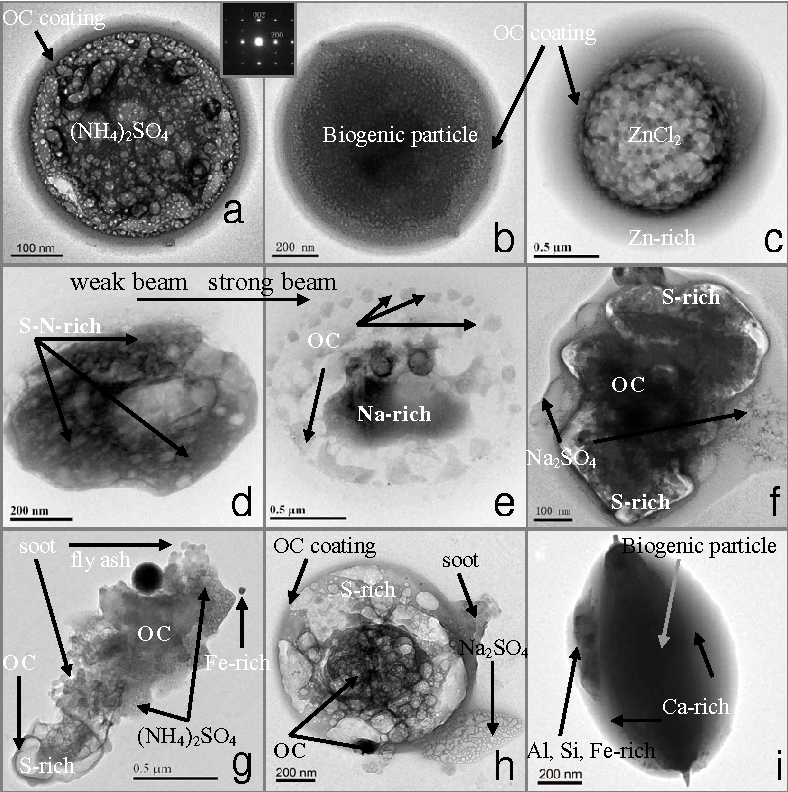
\includegraphics[scale=0.40]{chap1_figs/thesis_chap1_fig2.png}
	\caption{TEM images of carbonaceous particles collected from
          urban Shanghai, adapted from \cite{fu2012morphology}.}
	\label{fig:chap1-mixing}
\end{figure}

%Aerosol particles diameters range from several nanometers to over 10 $\rm \mu m$.  

In addition to exhibiting great diversity with respect to composition,
aerosol particle diameters vary from small molecule clusters of
several nanometers to large particles of several micrometers
\citep{MCMURRY200320}. It is common to represent the aerosol size
distribution by three size ranges, called ``modes'': The nuclei mode
(0.01--0.1 $\rm \mu m$), the accumulation mode (0.1--2 $\rm \mu m$)
and the coarse mode (2--10 $ \rm \mu m$). Nuclei-mode particles are
commonly observed near combustion sources, especially the roadside
atmosphere, and characterized by high number concentration, which
causes efficient coagulation and results in short lifetime of these
particles \citep{fushimi2008atmospheric}. Accumulation-mode particles
contain most of the secondary species, such as sulfate, nitrate and
organics \citep{zhang2005time}, and they can be produced from the
growth of nuclei-mode particles by coagulation and condensation. These
particles stay longer in the air because the removal processes of
coagulation and dry deposition are not efficient in this size range.
The lifetime of these particles can be up to one week
\citep{feichter2009climate}, with wet deposition being the most
efficient removal process. As for coarse-mode particles, it is hard to
grow such large particles directly from the accumulation mode
\citep{friedlander1991scavenging, lee2005size}. They mostly originate
from natural sources and produced through mechanical processes. Rapid
gravitational settling results in a short lifetime for these
particles.

\section{Aerosol climate forcing}
\label{cha1-2:aerosl-climate}
Aerosol impact the radiation balance of Earth system through direct
interactions with shortwave and longwave radiation. The globally
averaged direct aerosol effective radiative forcing between 1750 and
2011 is estimated to be $-$0.45 $\rm W$ $\rm m^{-2}$, as shown
in Fig.~\ref{fig:chap1-aerosol-climate}. Estimation of radiative
forcing relies on the properties of aerosol population, such as size
and chemical components. The large variation of aerosols in different
regions leads to spatial variation of this effect. For example, while
the direct radiative forcing at the top of atmosphere over Africa is
around $-$12 $\rm W$ $\rm m^{-2}$, it can reach $+$30 $\rm W$ $\rm
m^{-2}$ over the polluted Indo-Gangetic Plains
\citep{subba2020recent}.

\begin{figure}
	\centering
	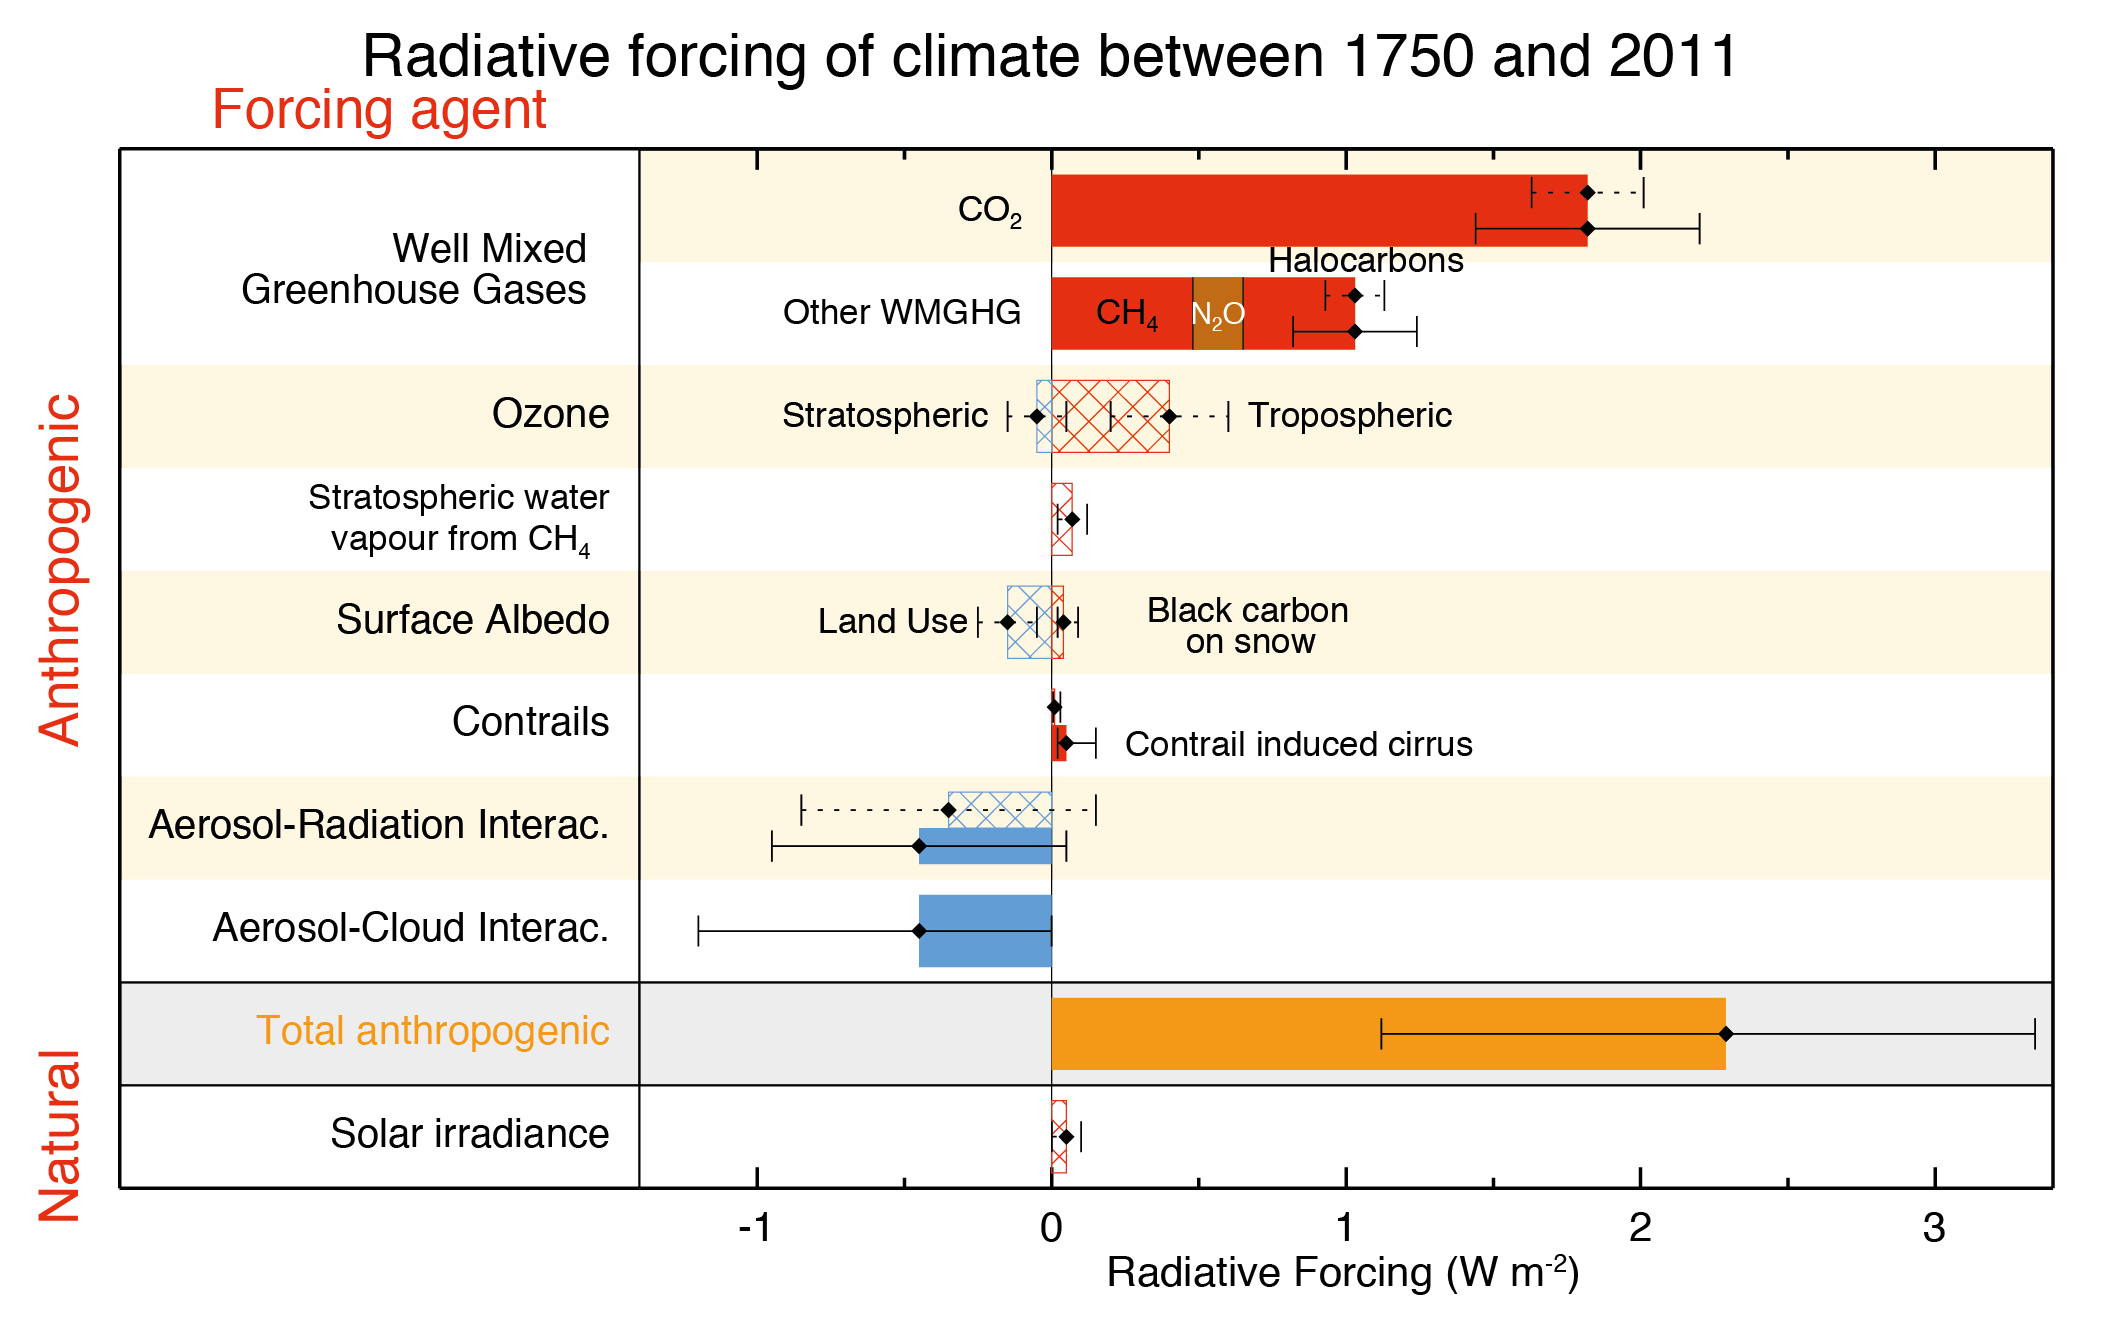
\includegraphics[scale=0.80]{chap1_figs/thesis_chap1_fig1.jpeg}
	\caption{Radiative forcing estimation of different agents between 1750 and 2011, adapted from \cite{IPCC_CHAPTER8}.}
	\label{fig:chap1-aerosol-climate}
\end{figure}

By serving as cloud condensation nuclei, aerosol particles also
indirectly affect climate through interactions with cloud, and the
estimated effective radiative forcing from this interaction is
$-0.45$~\unit{W\;m^{-2}}, similar to the effective direct radiative
forcing (Fig.~\ref{fig:chap1-aerosol-climate}). There are many
processes involved in the interactions, which can be summarized by two
main effects: the cloud albedo and the lifetime effects. However,
large uncertainties still exist in quantifying the cloud lifetime
effects, and they are not included in calculating aerosol-cloud
interaction forcings in Fig.~\ref{fig:chap1-aerosol-climate}.

Cloud albedo effects, first proposed by \citet{twomey1977influence},
describe the changes of cloud droplet number concentration and surface
area as the number concentration of aerosol particles changes, which
was supported by ambient observations. \citet{kaufman2005effect}, by
analyzing satellite observations in four regions over Atlantic ocean
where clouds are affected by four different types of aerosols, proved
that polluted clouds contain more smaller droplets. In-situ field
observations also confirm that more cloud condensation nuclei (CCN)
generate more cloud droplets with smaller sizes in liquid clouds
\citep{jia2019distinct,kleinman2012aerosol}.

The cloud lifetime effect describes the mechanism that the increase of
aerosol number concentration not only results in smaller cloud
droplets but also inhibits the precipitation development. This effect
is plausible if only the initiation of precipitation is
considered. However, several observation and modeling studies
suggested that it is hard to find clear evidence for this effect due
to the complex microphysical and macrophysical buffer responses after
altering the aerosol loading in the environment
\citep{stevens2009untangling}.
% May do not need to mention this because we are not going to talk about it. 
%The physical understanding of interactions with liquid cloud improves substantially in past decades, but the interactions with ice and mix-phased clouds is still poor constrained. 

As we can see from Fig.~\ref{fig:chap1-aerosol-climate}, large
differences still exist among different models in the magnitude of the
aerosol-related radiative forcing. For the radiative forcing from
aerosol radiation interaction, the estimated 5 to 95\% confidence
interval ranges from $-0.95$ to $+ 0.05$ $\rm W$ $\rm m^{-2}$, while
the range is from $-1.2$ to $0.0$ $\rm W$ $\rm m^{-2}$ for the
radiative forcing due to aerosol-cloud interaction. The sources of the
uncertainty lie in the fact that the processes involved cover a large
range of scales, from particles as small as 10~nm to 1000~km
stratocumulus clouds. Many processes are still not well-understood on
a fundamental level, such as aerosol interaction with mixed-phase and
ice clouds, and simple parameterization schemes are applied to
describe these processes in the models. But even for the processes
that are well-understood on a microscale level, it is challenging to
incorporate all them in a large-scale model
\citep{seinfeld2016improving,bellouin2020bounding}. By interacting
with electromagnetic radiation, and acting as an nuclei for cloud
formation, particles are fundamental for determining radiative forcing
and an accurate description of aerosols can help reduce the model
uncertainty or at least help quantify the uncertainty that is
currently present.

\section{Aerosol mixing state}
The aerosol mixing state refers to the distribution of chemical
species among a particle population and is a helpful framework to
describe aerosols \citep{winkler1973growth}. We distinguish between
two mixing state extremes: the fully internal mixture and the fully
external mixture. As Fig.~\ref{fig:chap1-chi-climate}(a) schematically
shows, a population is considered to be completely internally mixed if
each particle is made up of the same species mixtures, which equals
the bulk composition. For a population with fully external mixture,
each particle only contains one single species. However, in the real
ambient atmosphere, particles rarely fall into any of these two
categories but most likely assume one of many possible intermediate
mixing states. In other words, the number of species and their mass
fractions can differ between particles.

Hygroscopicity and optical properties, which are important factors for
droplets formation and the interaction with radiation, are both
strongly dependent on the chemical species that the particle consists
of. Thus, aerosol population with different mixing states may have
different climate-related properties, as illustrated in
Fig.~\ref{fig:chap1-chi-climate}. Figure~\ref{fig:chap1-chi-climate}(a)
explains this for the example of cloud condensation nuclei
activity. All three populations contain the same amount of ammonium
sulfate and organic matter, but the two species are distributed
differently among the particles. For the internally-mixed population,
each particle has the same amount of ammonium sulfate and organic. For
the externally-mixed population, each particle only contains one
single species. In the real environment, these two species can be
randomly distributed among the particles. If these three populations
are exposed at the same supersaturation (e.g., a supersaturation of
0.3\%), the number of activated particles will be different. All the
particles are activated in the population with internal mixture, while
only 50\% are activated in the externally mixed population. The
activated particles number in real world case are between these two
extremes.

\begin{figure}
	\centering
	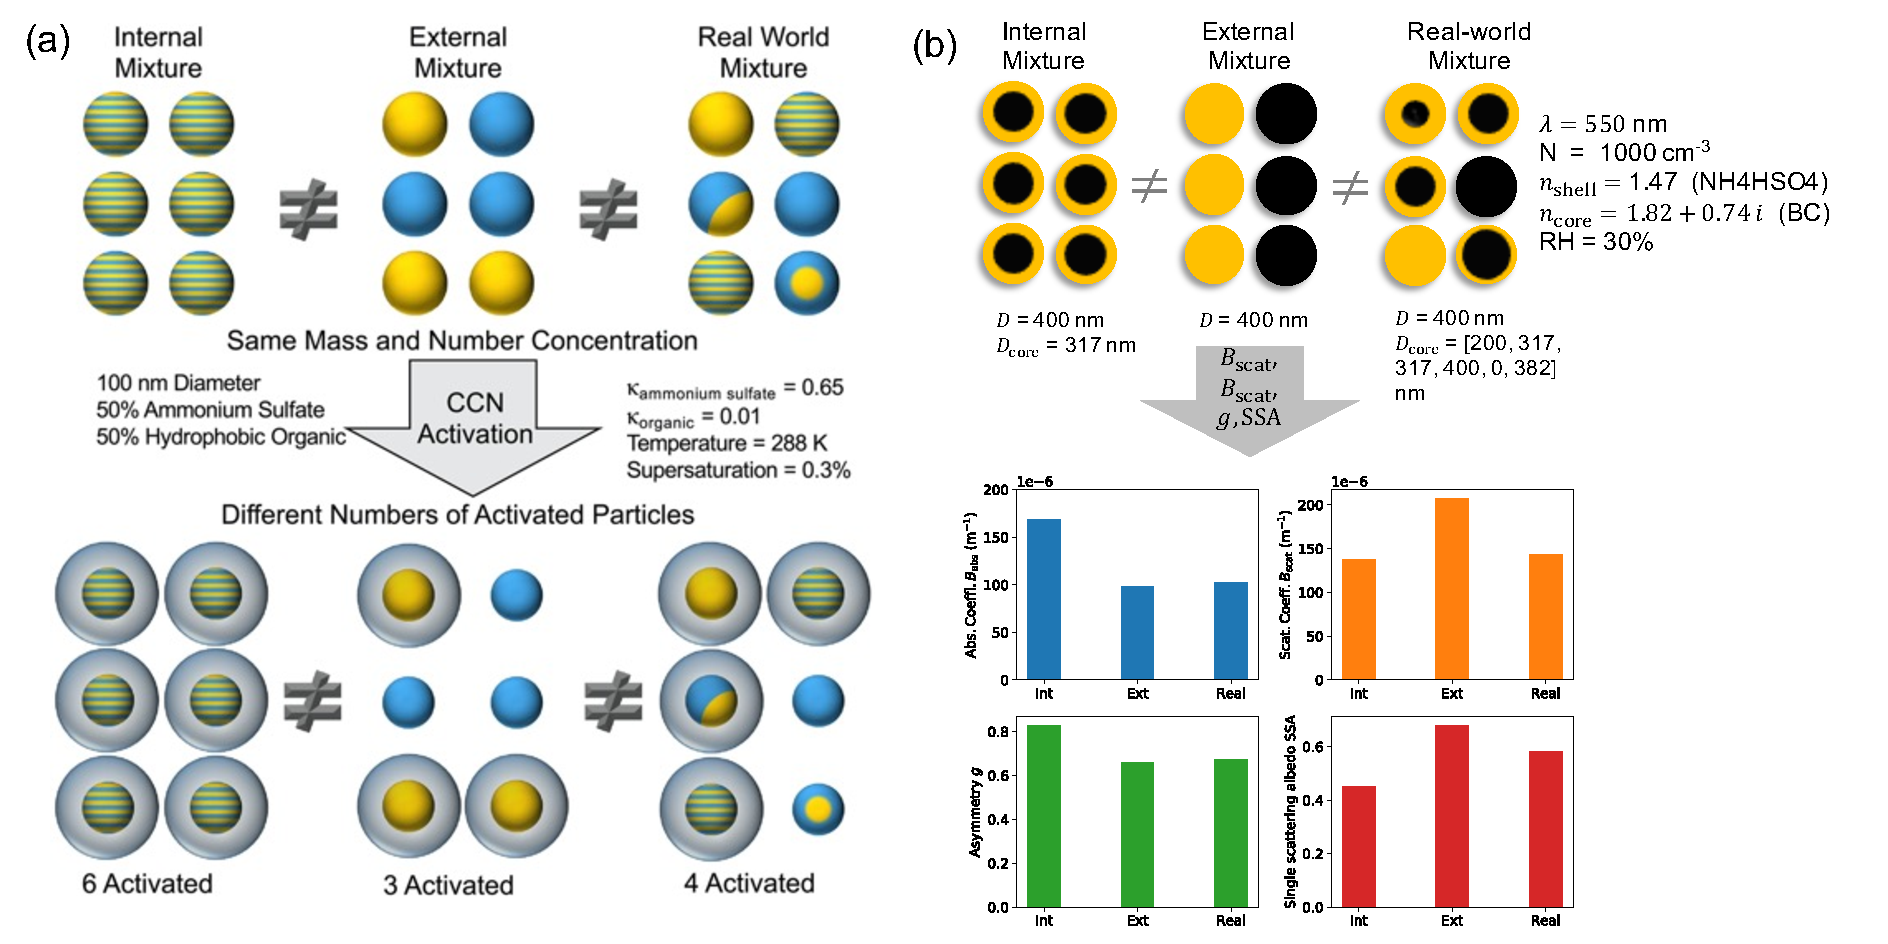
\includegraphics[scale=0.55]{chap1_figs/thesis_chap1_fig3.pdf}
	\caption{Aerosol mixing state effects on (a) activation
          ability and (b) optical values. (a) is adapted from
          \cite{Riemer2019}.}
	\label{fig:chap1-chi-climate}
\end{figure}

The effects of mixing state on aerosol activation potential has been
investigated through closure studies. An aerosol/CCN closure study is
conducted by comparing the observed and predicted CCN concentrations
at a given supersaturation level. The prediction is usually made by
applying K\"ohler theory, using the measured dry particle size
distributions and chemical composition information as input, with
assumptions in mixing state to examine its effects.
\citet{broekhuizen2006closure} performed such a closure study for
aerosol samples from downtown Toronto at 0.58\% supersaturation, and
they found the internal mixture assumptions overpredicted CCN
concentrations by 7--17\%. Using the CCN sampled from 2010 CalNex
field campaign, \citet{moore2012hygroscopicity} also found that
internal mixture resulted in 30--75\% overprediction of CCN
concentration. \citet{ervens2010ccn} conducted a comprehensive closure
study by using aerosol data collected from six different
locations. They found, for regions that are affected by fresh
emission, detailed size-resolved aerosol information are required to
make a reasonable CCN prediction, while for regions are with aged
aerosols, CCN can be well-predicted with simple (internally-mixed)
aerosol representations.

As for the effects on aerosol optical properties, we can apply the
same strategy as in Fig~\ref{fig:chap1-chi-climate}(a) to explain the
relevance of mixing state. Figure~\ref{fig:chap1-chi-climate}(b) shows
the populations with the same amount of absorbing species (BC) and
non-absorbing species ($\rm NH_4HSO_4$), but with different mixing
states. As a result, the optical properties, including single
scattering albedo (SSA), volume scattering coefficients ($\beta_{\rm
  abs}$) and volume absorption coefficients ($\beta_{\rm abs}$) are
different and can lead to different radiative forcing.

The effects of aerosol mixing state on its optical properties can be
more complicated if considering aerosol water uptake and particle
shapes. In a humidified environment, water update of a particle
depends strongly on its composition because of the dependence of
hygroscopicity on the chemical species, which is important for
scattering \citep{MichelFlores2012, Zieger2013, Titos2014,
  Titos2016}. Studies showed, compared with a dry environment, the
scattering ability can be enhanced by a factor of 1.6 at the
environment with RH of 85\% \citep{Burgos2020}. As for particle
shapes, the distribution of the diverse species {\rm within} a
particle is important in determining optical values. For particles
without strong absorber, i.e. BC, a volume-mixing rule can be used to
calculate the overall refractive index of the particle. When the
particle contains BC, assuming a core-shell configuration has been
shown to be more accurate \citep{Bond2006} than assuming a well-mixed
particle. The absorption enhancement of BC-containing particles due to
its coatings have been widely investigated \citep{Moffet2009,Liu2017,
  wu2020light}. The distribution of the non-absorbing species over the
population were found to be the main sources for the discrepancies
between the simulated and observed optical values \citep{Fierce2016,
  Fierce2020}. That is, in order to simulate absorption enhancement
correctly, it is important to know the coating thinkness for a given
population of BC cores. In particular, assuming an internal mixture
(where larger BC cores receive thicker coatings) leads to a systematic
overestimation of the absorption enhancement. Considering the
non-spherical shapes of BC-containing particles complicates the
calculation of optical properties considerably. By using the Discrete
Dipole Approximation (DDA) model, \citet{scarnato2013effects} found
that for mixed particles containing BC and NaCl, the absorption
coefficients enhancement is higher for internally mixed compact BC
than lacy BC. However, the computational cost for DDA calculations is
much higher than for Mie calculations.

\section{Aerosol mixing state evolution}  
Aerosol mixing evolution in the atmosphere involves several
processes. It is important to recognize that, at the time of emission,
particles can already be a mixture of different species. For example,
particles emitted from diesel engines are mixture of BC, primary
organics and sulfate, and sea-spray aerosols are a mixture of sodium
chloride and organics \citep{cheung2010emissions,
  kirpes2018secondary}. Once emitted, the mixing state can be further
modified by condensation of organic or inorganic low-volatility
compounds.
%Heterogeneous reactions between gas-phase reactants and
%condensed-phase surface can be faster than reactions in gas-phase,
%and one important reaction is the ozone depletion by chlorine radials
%produced from heterogeneous reactions between chlorofluorocarbons and
%polar cloud surface \citep{davies2018heterogeneous}.
Coagulation between particles is an efficient process for changing
particle number concentration, and Brownian coagulation was shown to
be the main reason for the rapid evolution of soot particle size
distribution near a highway \citep{jacobson2004evolution}. The
coagulation process alone will make the particle composition more
similar, and particle population undergoing coagulation will become
more internally mixed \citep{Riemer2013a}.

The processes of condensation and coagulation outlined above are
relevant for a cloud-free environment, however, since the global cloud
coverage is on average more than 70\%
\citep{stubenrauch2013assessment}, the aerosol evolution in clouds is
also an important contributor during the lifetime of aerosol
populations, and motivates the work presented in Chapter~\ref{chap2}
and Chapter~\ref{chap3} of this thesis. Figure~\ref{fig:chap1-aq-proc}
shows the chemical and physical processes particles experience in fogs
and clouds. When the atmosphere reaches supersaturation, particles
with critical supersaturation lower than the environment
supersaturation are activated as cloud droplets and undergo nucleation
scavenging. For these activated particles, the absorbed water
facilitates aqueous chemical reactions. Gas species dissolve in the
cloud droplet, and if both liquid and ice phases exist in the cloud,
species partition between the two phases and the retention
coefficients in the liquid phase are varied. When cloud droplets grow
to rain droplets, they precipitate. During precipitation, small
interstitial aerosol particles can be collected by these large
droplets and impaction scavenging occurs. For clouds with strong
convection, gas and particle species are vertically redistributed by
convective transport.

\begin{figure}
	\centering
	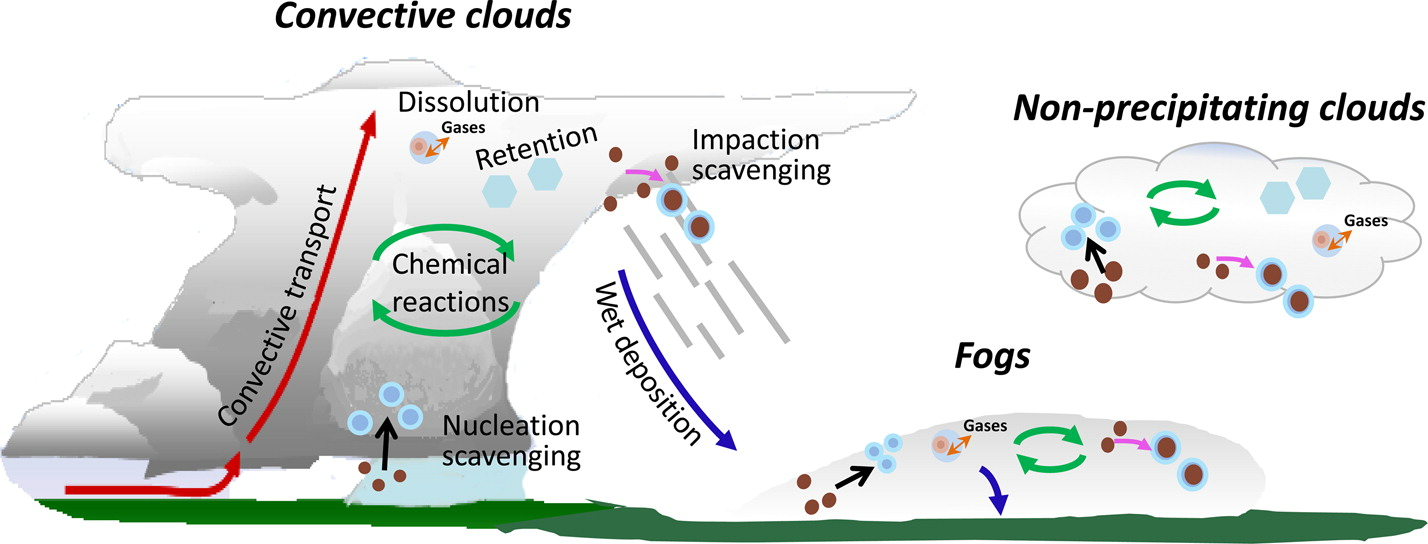
\includegraphics[scale=1.0]{chap1_figs/thesis_chap1_fig4.jpeg}
	\caption{Chemical and physical processes involved in fogs and
          clouds, adapted from \cite{ervens2015modeling}.}
	\label{fig:chap1-aq-proc}
\end{figure}

The aqueous phase in clouds provides an efficient medium for sulfate
formation. Globally, more than 50\% of sulfate forms through in-cloud
oxidation and the formation rates of aqueous reactions, $\rm SO_2$
oxidation by $\rm H_2O_2$ and $\rm O_3$, are more effective than
through OH oxidation in gas phase \citep{kreidenweis2003modification,
  rasch2000description}. Other aqueous sulfate formation mechanisms,
such as the reactions catalyzed by Transition Metal Ions (TMI), can
also be important. For example, reaction cycles involving TMI have
been shown to be the dominant pathway for sulfate formation in the
samples collected during HCCT-2010 field campaign
\citep{harris2012sulfur, harris2013enhanced}.

%Reaction rates of aqueous processes rely on cloud properties and the
%importance of different pathways differs at various cloud types.
%\citet{straub2007chemical}, analyzing the marine stratocumulus cloud
%samples collected over eastern Pacific Ocean during DYCOMS-II field
%campaign, found $\rm SO_2$ oxidized by $\rm H_2O_2$ is the dominant
%reaction for sulfate production.
In addition to sulfate, aqueous reactions can also form SOA. Globally,
SOA produced from aqueous pathway can reach to 20--30 Tg·$\rm
yr^{-1}$. Glyoxal, methylglyoxal, glycolaldehyde and acetic acid can
act as the precursors for aqueous SOA \citep{liu2012global}. As for
the oxidants, besides hydroxyl radical, which is the dominant oxidant
for SOA formation at gas phase, aqueous environment can provide
several other efficient oxidants, such as peroxyl radicals, peroxides
and triplet excited states of organic compounds ($^{3}\textrm{C}^*$)
\citep{mcneill2015aqueous, ervens2011secondary}. Using simulated
sunlight UV, \citet{smith2014secondary} found phenols can be rapidly
oxidized by $^{3}\textrm{C}^*$ to produce low-volatility SOA .

The aerosol size distribution evolves after the formation of aqueous
inorganic and organic species. The characteristic ``Hoppel minimum''
describes the gap between two particle distribution modes at
approximately 0.02--0.03 and 0.08--0.15~$\rm \mu m$
\citep{Hoppel1986}, evident in particle populations processed by
non-precipitating clouds. After being described for the first time by
\citet{Hoppel1986}, this phenomena has further been observed for
aerosol populations in different regions, such as during the VOCALS
campaign over west Chilean coast \citep{kleinman2012aerosol} and the
MASE campaign at the central California coast
\citep{hudson2015cloud}. Besides the formation of secondary aerosol
through aqueous phase reactions, particle size distributions also
changes due to coagulation between interstitial particles and cloud
droplets. \citet{pierce2015importance} found that this process can
reduce total particle number concentration by 10--15\% globally.

The evolution of mixing state in turn affects the aerosols'
climate-related properties. \citet{Ching2016} found that for polluted
environments where BC-containing particles age quickly, increased BC
emissions result in larger cloud droplet number concentrations (even
though fresh BC particles are poor CCN). Aerosol optical properties
are altered as mixing state evolves, especially for BC-contained
particles. As mentioned above, the absorption enhancement of
BC-containing particles due to coatings of non-absorbing species are
widely confirmed by models, laboratory studies and field observations
\citep{Moffet2009,Liu2017,wu2020light,Fierce2020}.

Considering the importance of mixing state for describing an aerosol
population, a qualitative description using the terms, such as
internal or external mixture, are limited in quantifying the effects
of mixing state. \citet{Riemer2013a}, based on the theory of
information-theoretic entropy, developed the index $\chi$ to quantify
aerosol population mixing state. The index $\chi$ is the ratio between
average particle diversity $D_{\alpha}$ and bulk diversity
$D_{\gamma}$. By using particle mass measurement data, these metrics
were successfully proved to be capable of explaining the aerosol aging
processes \citep{Healy2014}. They are also an important framework for
our analyses presented in Chapter~\ref{chap3} and Chapter~\ref{chap4}.


\section{Aerosol modeling approaches}
The application of a variety of aerosol measurement techniques helps
advance our understanding of aerosol particles, and we know that the
observed particles are the consequence of multiple chemical and
physical processes. By using numerical models, we can isolate the
underlying individual processes, and predict what will happen if
certain processes change. Considering the wide range of chemical
species and particle sizes in an aerosol population, it is hard for a
single model to represent all possible processes the population can
experience during its lifetime, from emission to deposition, and
balance need to be reached between model accuracy and computational
efficiency. This section summarizes the current aerosol modeling
approaches from simplistic bulk methods used in some global models to
comprehensive particle-resolved models used in box model. We will
focus on how these models deal with aerosol mixing state and its
implication for aerosol-related climate properties.

\subsection{Bulk models}
The simplest aerosol modeling approach is the so-called bulk
method, as shown in Fig.~\ref{fig:chap1-aerosol-model}(a). 
Aerosol populations are represented by the mass concentrations
of several common aerosol species, such as sulfate, BC, organic
aerosol, dust and sea salt, and these species are treated as external
mixtures in the bulk without detailed information about how the
species may be mixed with each other. Rather than tracking the aerosol
evolution through microphysical processes, this approach prescribes
the aerosol size distribution from climatologal data. This approach is
computationally very efficient and applied by several global models,
such as GOCART \citep{chin2000atmospheric} and TM5
\citep{vignati2010sources}.

\subsection{Modal models}
A more advanced approach is representing the aerosol populations by
several overlapping distributions, also called modes, as shown in
Fig.~\ref{fig:chap1-aerosol-model}(b). A modal model tracks the size
distribution evolution of the modes. Each mode can contain a variety
of aerosol species. Within each mode, all species are assumed to be
internally mixed. Since the modes can overlap in certain size ranges,
mixing state can be represented at least in a simplified way,
especially when many modes are used \citep{Bauer2008}. Lognormal functions are
typically used to represent the number distribution of each mode as
follows:
\begin{equation}
\centering
    n({\rm log}D_p) = \sum_{i=1}^{m}\frac{N_i}{\sqrt{2\pi}{\rm log}\sigma_i}{\rm exp}(-\frac{({\rm log}D-{\rm log}{\overline{D}_i})^2}{2{\rm log}^2\sigma_i}),
\end{equation}
where $m$ is the number of modes, $N_i$ is the total number
concentration of mode $i$, $\overline{D}_{i}$ and $\sigma_i$ are the
geometric mean diameter and geometric standard deviation of mode $i$,
respectively.

The number of modes can vary among different models. Aitken,
accumulation and coarse modes are the essential three modes, and this
configuration is for example used in the ECHAM4 global climate model
\citep{lauer2005simulating} and in the regional chemistry 
transport model \citep{binkowski2003models}. 
Other models introduce additional modes to better
represent hydrophilic and hydrophobic species. For example, MAM7 used
in the CAM5 global model applies an additional primary carbonaceous
mode that represents primary organic matter and BC, which has lower
hygroscopicity than the accumulation mode \citep{liu2012toward} that
also contains sulfate and SOA. For the three parameters used to
describe the lognormal distribution, standard deviation of each mode
is typically prescribed, and total number concentration and geometric
mean diameter change as the aerosol evolves.

\begin{figure}
	\centering
	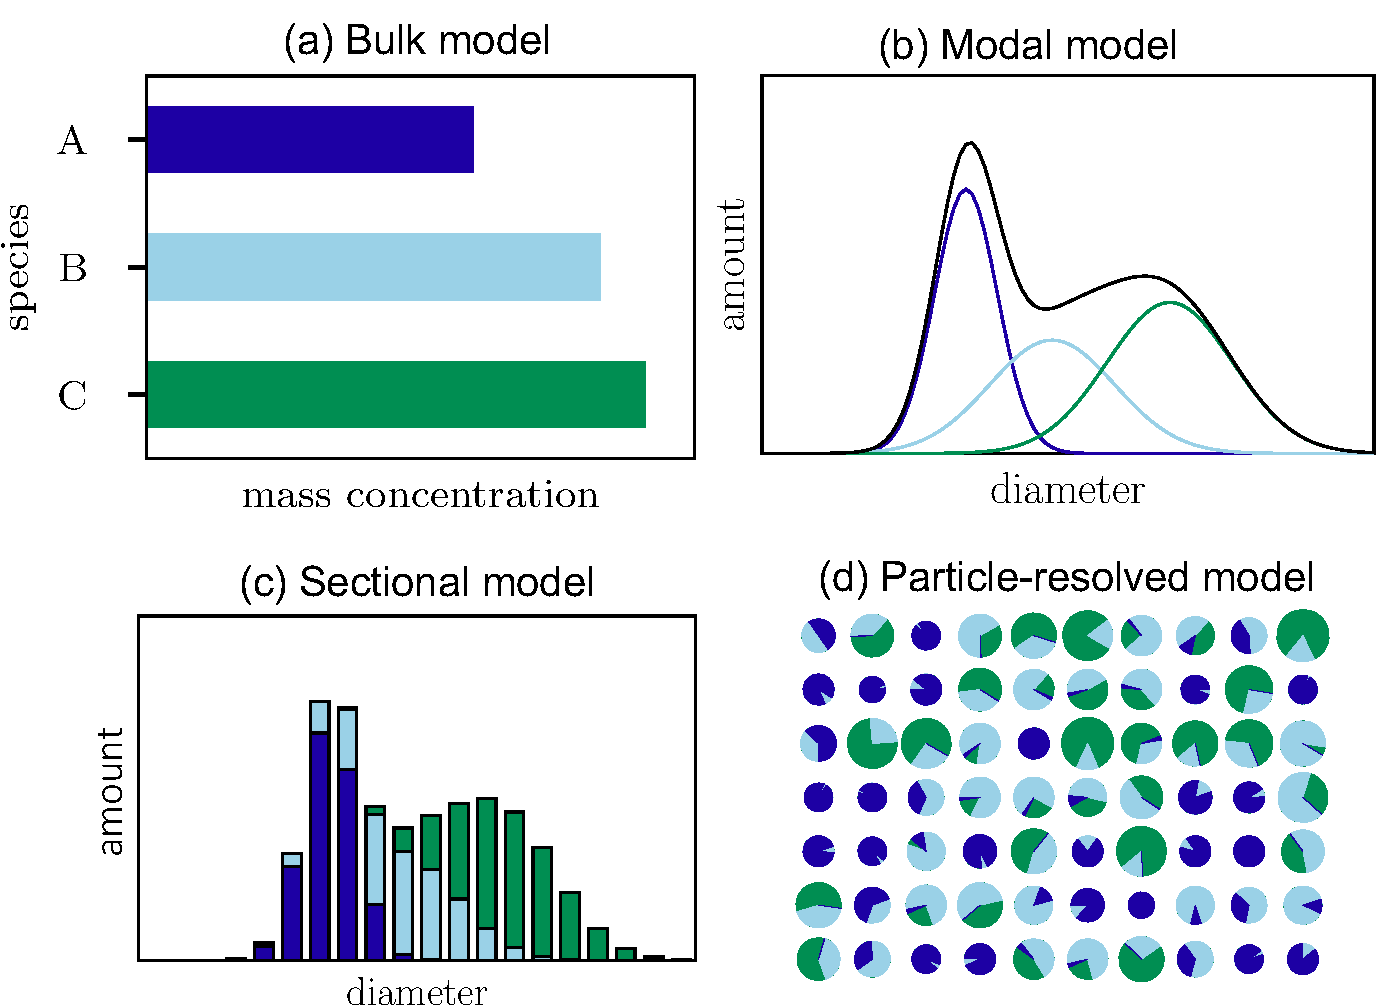
\includegraphics[scale=0.5]{chap1_figs/thesis_chap1_fig5.pdf}
	\caption{Aerosol numerical approaches:(a) Bulk model, (b) Modal model, (c)
          Sectional model, and (d) Particle-resolved model.}
	\label{fig:chap1-aerosol-model}
\end{figure}

\subsection{Sectional models}
Similar to modal methods, sectional aerosol models are also
distribution-based. Instead of tracking the population by different
modes, this approach discretizes the distribution into a certain
number of size bins and then track the changes in each bin, as
illustrated in Fig.~\ref{fig:chap1-aerosol-model}(b). Particles are
internally mixed within each bins and the composition can vary between
bins. The sectional approach is widely applied to large-scale
models. For example, the sectional model MOSAIC is extensively used in
WRF-Chem with 4-bin and 8-bin versions available, and proved to
capture the summer particulate matter distribution well over the
Houston region \citep{zaveri2008model,fast2006evolution}. The TOMAS
sectional model is applied to several global chemistry models, such as
GEOS-Chem, and improved its ability in simulating aerosol optical
properties recently through more detail mixing state representation of
particles
\citep{adams2002predicting,pierce2013weak,kodros2018size}. TOMAS uses
30 bins and covers the diameter range between 0.01 and 10 $\rm \mu m$.

Most sectional models apply univariate distributions and use
assumptions for the aerosol mixing state in each bin. Some more
advanced schemes have been developed to incorporate more information
within each size bin, especially for representing a variable BC mass
fraction within each size bin. Based on the Model of Aerosol Dynamics,
Reaction, Ionization, and Dissolution (MADRID) module,
\citet{oshima2009aging} developed a two-dimensional sectional scheme
MADRID-BC by adding another dimension for BC mass fraction and
tracking the fraction changes due to condensation/evaporation
processes. Through developing MOSAIC-MIX, \citet{ching2016three}
further extended the sectional model representation by incorporating
another dimension for hygroscopicity, and coagulation process had been
added to evaluate its effects on BC mixing state.

\subsection{Particle-resolved models}
Even though modal and sectional models provide better representation
of particle size distributions than bulk models, aerosol mixing state
still needs to be represented in a simplified way by using internal or
external assumptions. A more advanced representation of aerosol mixing
state is the particle-resolved method, as illustrated in
Fig.~\ref{fig:chap1-aerosol-model}(c). Rather than using distributions
to represent the population, a particle-resolved model samples the
population with discrete computational particles. Specifically, each
particle is represented by an $A$-dimensional vector, where $A$ is the
total species number. The first particle-resolved aerosol model for
the ambient atmosphere was developed by \citet{Riemer2009} and it was
coupled with the MOSAIC module to include gas-particle partitioning
and gas chemistry processes. The model was applied to investigate the
aging process of BC-containing particles in a urban plume environment
and the evolution of ship plume particles \citep{tian2014modeling,
  Ching2016}. Recently, PartMC-MOSAIC had been further coupled with
WRF-chem to track the particle evolution for a large-scale domain
\citep{curtis2017single}. However, MOSAIC only considered aerosol
aging process for subsaturated environments (RH < 100\%). It can not
be used to investigate the chemical processes in a cloud
environment. Extending and applying the PartMC modeling framework to
include aqueous phase chemistry is one of the goal for this
thesis. More details about PartMC will be presented in
Chapter~\ref{chap2}.

In summary, the bulk model approach is the most simplified method with
mixing state being represented by an external mixture of different
particle types. Modal and sectional models represent aerosol
populations by distributions. Their ability to describe aerosol mixing
state is limited by the number of modes or bins included in the models
and they still rely on assumptions for mixing state within modes or
bins. With the particle-resolved approach, each computational particle
is explicitly tracked and the mixing state of aerosol population is
accurately represented.

\section{Models for aqueous chemistry simulation }
One of the topics for the thesis is to investigate the impact if
aqueous phase chemistry on aerosol mixing state. The previous section
discussed different approaches to simulate aerosol composition and
represent mixing state. This section summarizes how aqueous phase
chemistry mechanisms are incorporated into models. From particle
activation at nanometer scale to stratocumulus structures over
thousand kilometers, cloud processes cover around $10^{14}$ orders of
magnitude, and it is infeasible for a single model to incorporate all
the related processes. Models with aqueous processes can be divided
into two groups: process model with explicit aerosol microphysics and
complex aqueous chemical mechanisms, and
large-scale model with simplified representation of cloud properties
and processes.

For process models, often used as box/parcel models, aerosol
microphysics is usually well-resolved. Droplet activation is
explicitly described by using K$\rm \ddot{o}$hler
theory. Specifically, particles with critical supersaturation lower
than maximum supersaturation reached in the environment are activated
as droplets \citep{rothenberg2016metamodeling,
  ching2012impacts}. Detailed aqueous chemistry processes can be
incorporated into these cloud parcel models. An example is the cloud
parcel model SPACCIM coupled with the detailed aqueous scheme CAPRAM
(492 species and 1087 reactions in version 3.0). It has been
successfully compared to measurements during the FEBUKO campaign
\citep{wolke2005spaccim}. Since particle size distributions are
commonly described in process models, the modification of the size
distribution after cloud processes can also be captured. The
limitation of these models is the lack of the interactions with the
cloud dynamics. 

It is hard to include such detailed process information in global
models where computational efficiency is very important. Rather than
resolving cloud microphysics explixcitly, cloud properties are
described in a highly parameterized way, by using cloud fraction, with
other diagnosed meterological parameters, for each grid box. Cloud
droplet sizes distributions are usually assumed. For example,
ECHAM5-HAM assumed two bins for the cloud droplets: one bin for
particles with lower ion concentration and the other bin for high ion
concentration. As for the effects of cloud droplets representation on
cloud chemistry, \citet{barth2006importance}, by comparing sectional
and single-size droplet parcel model, found simplified cloud droplet
size representation will lead to biases in simulated formic acid and
formaldehyde concentration. Simplified aqueous mechanisms are also
used and the acidity, which is an important factor for aqueous
chemistry, are fixed at constant value. For example, GEOS-Chem used a
pH of 4.5 for $\rm SO_2$ oxidation reaction by $\rm
O_3$\citep{park2004natural}. Furthermore, assumptions need to be made
to consider the distribution of species produced from aqueous
reactions. For example, in CMAQ, all the non-volatile aqueous-formed
species are added to accumulation mode after cloud dissipates
\citep{binkowski2003models, fahey2017framework}.
 
%\begin{table}
%\setlength\extrarowheight{5pt}
%\centering
%\caption{Overview of acidity, mixing state and optical calculation treatment in different models}
%\label{tab:input}
%\begin{tabular}{ c c c c c}
%	\hline
%	Model acronym  & Model scale &  pH  &  mixing state & Optical calculation  \\
%	\hline
%    CMAQ & Regional & Equilibrium pH & Internal mixture in each mode & \\
%    WRF-Chem (MOSAIC) & Regional  & Equilibrium pH & Internal mixture in each bin &\\
%    GEOS-Chem (TOMAS) & Global & fixed pH at 4.5 & Internal mixture in each bin & \\
%    MOZART & Global & pH based on charge balance &  & \\
%    ECHAM5-HAM & Global & 
%    \begin{tabular}{@{}c@{}}pH based on initial aerosol \\ at small and large droplets\end{tabular} & Internal mixture in each mode & \\
%    PartMC-MOSAIC & 0-D & \begin{tabular}{@{}c@{}}pH based on detailed \\ mechanism at CAPRAM 2.4\end{tabular} & particle-resolved & \\
%	\hline
%   \end{tabular}
% \end{table}
\section{Research questions and thesis organization}
Aerosol particles affect climate forcing through directly altering
radiation and indirectly interactions with clouds. These effects are
dependent on the particles' chemical composition, in other words, the
chemical species mixing state of the aerosol population. The objective
of this dissertation includes two parts: quantifying cloud chemical
processes and their impact on mixing state, and quantifying the
effects of aerosol mixing state on aerosol optical properties. 

For the first part, I will focus on the following scientific
questions: (1.1) To what extent does cloud
processing change the aerosol mixing state of the population that
entered the cloud?  (1.2) How does this change the cloud condensation
number concentration and optical properties? (1.3) What is the
implication of coagulation between the interstitial particles and
cloud droplets for mixing state of aerosol population?

For the second part, the following two questions will be addressed:
(2.1) What are the errors in aerosol optical properties introduced by
internal mixture assumptions used in sectional models? (2.2) How does
this error depend on relative humidity and associated water uptake of
the aerosol?

Both objectives are addressed with a particle-resolved modeling
approach. Chapter~\ref{chap2} describes the coupling of the particle-resolved
model PartMC-MOSAIC with the aqueous mechanism
CAPRAM. Chapter~\ref{chap2} also presents the results from idealized
model simulations to confirm expected sensitivities of sulfate
formation to model input parameters.

Chapter~\ref{chap3} investigates the cloud processing effects on aerosol
properties. In this work, I used a typical urban plume particle
population to experience several idealized cloud cycles to determine
the changes of aerosol mixing state and quantify the changes of
aerosol microphysical and optical properties after the cloud
evaporates. Another simulation is conducted to identify the role of
coagulation between cloud droplets and interstitial particles. This
chapter will answer questions 1.2--1.4. A paper entitled ``The impacts
of cloud processing on resuspended aerosol particles after cloud
evaporation'', which is in review for \textit{Journal of Geophysical
  Research-Atmosphere}, summarizes the results on the changes of
aerosol microphysical properties after cloud processing. Another
paper, which is entitled with ``Quantifying the Effects of Cloud
Processing on Aerosol Optical Properties Using a Particle-Resolved
Model'' about the changes of optical properties after cloud
processing, is in preparation for \textit{Aerosol Science and
  Technology}.

Chapter~\ref{chap4} evaluates the error in aerosol absorption and
scattering, introduced by the internal mixture assumptions used in
sectional aerosol models. The error is quantified by comparing the
aerosol optical value differences between reference populations
created by running particle-resolved model and sensitivity populations
with reduced representation of mixing state created by
composition-averaging methods. This chapter will answer the two
questions pertaining to the second part and a publication is in
preparation for \textit{Atmospheric Chemistry and Physics}, entitled
``Quantifying the effects of mixing state on aerosol optical
properties''.

Chapter~\ref{chap5} summarizes the main findings of this thesis and discusses
implications for resolving aerosol mixing state in the future for
global models.
%%%%%%%%%%%%%%%%%%%%%%%%%%%%%
%%%%%%%%%Chapter 2%%%%%%%%%%%
%%%%%%%%%%%%%%%%%%%%%%%%%%%%%
\chapter{Particle-resolved modeling of aqueous-phase chemistry}
\label{chap2}
This chapter presents the application of PartMC as a particle-resolved
cloud parcel model that includes aqueous-phase chemistry. I first
describe the PartMC model framework, and the coupled cloud parcel and
aqueous chemistry module as it was used in both this chapter and
Chapter~\ref{chap3}. Then, I present a comparison to other
size-resolved and bulk cloud chemistry models. Furthermore, I show
results from an ensemble of idealized scenarios that were designed to
confirm the sensitivity of aqueous sulfate formation to the
concentrations of oxidants and to transition metal ions.

\label{chap2:mon}
%%% Suggested section heads:
\section{Introduction}

Clouds cover around 70$\%$ of the earth
\citep{stubenrauch2013assessment} and create an environment for
multiphase reactions to occur \citep{Deguillaume2005}. Gas phase
species are taken up by cloud droplets and undergo aqueous-phase
chemistry. Oxidation of dissolved gases in the aqueous phase can
contribute to a large fraction of secondary inorganic and organic
aerosol. Globally, over 50\% of sulfate is produced through aqueous
reactions in clouds \citep{Philip2014, Roth2016}. If the cloud
evaporates, an aerosol population is released that has different cloud
condensation nuclei properties and optical properties compared to the
aerosol that formed the cloud \citep{Farmer2015, Henning2014}.

Particles with different composition and size experience different
effects from aqueous-phase chemical processing. First, particle size
and composition determine which particles can be activated and form
cloud droplets. Second, some aqueous-phase sulfate formation reactions
are highly pH-dependent, and the reaction rates for particles with
different acidity can vary by several orders in magnitude. For
example, transition metal ions (TMI), including Fe and Mn ions, which
mostly originate from mineral dust \citep{alexander2009transition},
catalyze aqueous sulfate oxidation reactions. The related pathways
become dominant when the pH is larger than 6.0
\citep{Seinfeld2006a}. It had been shown that at some cloud events,
the $\rm SO_2$ oxidation reaction catalyzed by coarse mineral dust TMI
can be more efficient than the oxidation by $\rm H_2O_2$
\citep{Harris2013a, Harris2014}.

Despite the potential importance of particle heterogeneity in
aqueous-phase chemistry, most regional or global models use simplified
assumptions to simulate aqueous processes. The global chemistry
transport model GEOS-Chem uses less than 10 dissolved species calculate
acidity \citep{alexander2012isotopic}. The regional chemical transport
model CMAQ tracks cloud chemistry processes for three lognormal modes,
neglecting the heterogeneity within each mode
\citep{fahey2017framework}. In this work, I applied the
particle-resolved model PartMC-MOSAIC \citep{Riemer2009, Zaveri2010a},
which tracks individual computational particles. The model has been
widely used to study aerosol aging processes in a cloud-free
environment \citep{Zaveri2010a,fierce2015explaining}. It has also been
used as a cloud parcel model to investigate the impact of aerosol
mixing state on cloud droplet formation \citep{ching2012impacts,
  Ching2016}. However, the model did not have the capability to
simulate aerosol aging due to aqueous-phase chemistry within
clouds. This is the focus of this chapter.

The remainder of this chapter is structured as
follows. Chapter~\ref{chap2.2} describes the PartMC modeling framework
used for this thesis. Chapter~\ref{chap2.3} compares results from the
particle-resolved aqueous-phase chemistry model with results from
existing literature. Chapter~\ref{chap2.4} explores the sensitivity of
sulfate formation to input parameters using an ensemble of idealized
simulations. The role of TMI pathway is further explored in
Chapter~\ref{chap2.5}. Findings are summarized in
Chapter~\ref{chap2.6}.

\section{Model description and simulation setup}
\label{chap2.2}
The model simulations presented in Chapter~\ref{chap2} and~\ref{chap3}
follow the two-step strategy described in \citet{ching2012impacts} and
illustrated in Figure~\ref{chap2-fig1-frame}. For the first step, I
simulated urban plume scenarios in a cloud-free environment using
PartMC-MOSAIC. The purpose of these simulations was to produce many
aerosol populations with a wide variety of aerosol mixing
states. These simulated aerosol populations were then used as the
input for cloud parcel simulations, including aqueous-phase chemistry,
in Step 2. Details about PartMC-MOSAIC, the cloud parcel model and the
aqueous-phase chemistry are described in the following sections.

\begin{figure}[ht]
    \centering 
    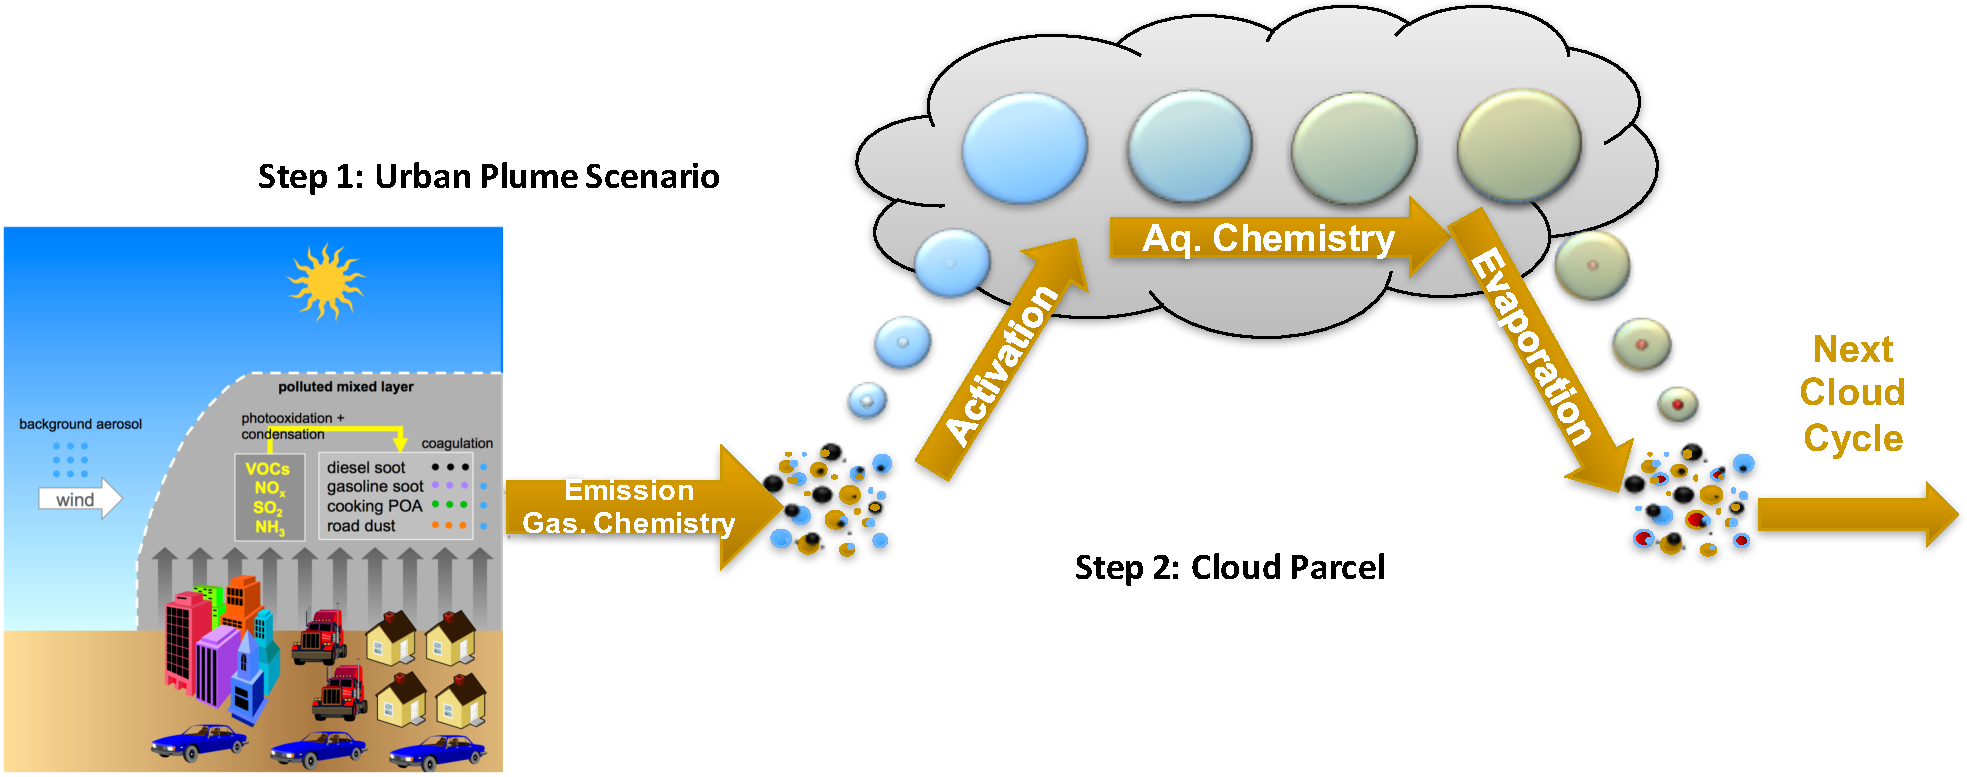
\includegraphics[scale=0.4]{chap2_figs/chap2-fig1-frame.pdf}
    \caption{Two-step particle-resolved modeling framework. Step 1 is
      the simulation of an urban plume scenario in a cloud-free
      environment. Step 2 is the cloud parcel simulation using output
      from the Step-1 urban plume simulations as input.}
    \label{chap2-fig1-frame}
\end{figure}

\subsection{The particle-resolved aerosol model PartMC-MOSAIC}
PartMC-MOSAIC (Particle Monte Carlo-Model for Simulating Aerosol
Interactions and Chemistry) is a Lagrangian box model which simulates
the evolution of individual computational particles in the ambient
atmosphere. The evolution is simulated assuming a well-mixed
computational volume and the particles' spatial positions are not
stored. The composition of each particle is tracked by representing
the particle as an $A$-dimension vector $\vec{\mu}^i \in \mathbb{R}^A$
with components ($\vec{\mu}_1^i,\vec{\mu}_2^i,...,\vec{\mu}_A^i$),
where $\vec{\mu}_a^i$ is the mass of species $a$ in particle $i$, with
$a$ = $1,...,A$ and $i$ = $1,...,N$. The evolution for aerosol number
concentration with species mass $\mu$ at time $t$, $n(\vec{\mu},t)$, 
is described by:
\begin{equation}
\begin{aligned}
 \frac{\partial n(\vec{\mu},t)}{\partial t} &= \underbrace{\frac{1}{2}\int_0^{\mu_1}\int_0^{\mu_2}...\int_0^{\mu_A} K(\vec{\mu}',\vec{\mu}-\vec{\mu}')n(\vec{\mu}',t)n(\vec{u}-\vec{u}',t)d{\mu_1}'d{\mu_2}'...d{\mu_A}'}_\text{coagulation gain}\\
& - \underbrace{\int_0^\infty\int_0^\infty...\int_0^\infty K(\vec{\mu},\vec{\mu}')n(\vec{\mu},t)n(\vec{\mu}',t)d\mu_1'd\mu_2'...d\mu_A' }_\text{coagulation loss} + \underbrace{\dot{n}_{\rm emit}(\vec{\mu},t)}_\text{emission} + \underbrace{\lambda_{\rm dil}(t)(n_{\rm back}(\vec{u},t))-n(\vec{\mu},t)}_\text{dilution}\\
&-\underbrace{\sum_{i=1}^{C}\frac{\partial}{\partial\mu_i}(c_iI_i(\vec{\mu},\vec{g},t))n(\vec{\mu,t})}_\text{gas-particle transfer} - \underbrace{\frac{\partial}{\partial\mu_{C+1}}(c_wI_w)(\vec{\mu},\vec{g},t))n(\vec{\mu,t})}_\text{water transfer} + \underbrace{\frac{1}{\rho_{\rm dry}(t)}\frac{d\rho_{\rm dry}(t)}{dt}n(\vec{\mu},t)}_\text{air density change},
\end{aligned}
\label{eq:partmc}
\end{equation}
where $K$ is the coagulation rate between the particles, $\dot{n}_{\rm
  emit}(\vec{\mu},t)$ is the emitting distribution of species
$\vec{\mu}$, $\lambda_{\rm dil}$ is the dilution rate with background
species concentration $n_{\rm back}$, $c_i$ is the gas to particle
conversion rate, $I_i$ is the gas species condensation flux, $c_{\rm
  w}$ is the gas to water conversion rate and $I_{\rm w}$ is the water
condensation flux.

The evolution of gas species $g_i$ at time $t$ is given by:
\begin{equation}
\begin{aligned}
 \frac{dg_i(t)}{dt} &= \underbrace{\dot{g}_{{\rm emit}, i}(t)}_\text{emission} + \underbrace{\lambda_{\rm dil}(t)(g_{{\rm back},i}(t) - g_i(t))}_\text{dilution} + \underbrace{R_i(\vec{g})}_\text{chemical reactions} + \underbrace{\frac{1}{\rho_{\rm dry}(t)}\frac{d\rho_{\rm dry}(t)}{dt}g_i(t)}_\text{air density change} \\
 & - \underbrace{\int_0^\infty\int_0^\infty...\int_0^\infty I_i(\vec{u},\vec{g},t)n(\vec{u},t)d\mu_1d\mu_2...d\mu_A}_\text{gas-particle transfer},
\end{aligned}
\label{eq:partmc-gas}
\end{equation}
where $\dot{g}_{{\rm emit}, i}(t)$ represents gas species $i$ emitting rate, $g_{{\rm back},i}$ is for gas species $i$ background concentration, and ${R_i(\vec{g})}$ is the gas species $i$ production rate from chemical reactions. 

The evolution processes represented in equation~\ref{eq:partmc} alter
the aerosol population by two mechanisms. By adding or removing
particles from the population, emission, dilution and coagulation
processes modify the number concentration of the population and these
processes are accomplished by PartMC with a stochastic Monte Carlo
approach. In addition, the composition of each particle can be altered
by species condensation and evaporation, which are simulated by the
state-of-art aerosol chemistry module MOSAIC. In MOSAIC, gas phase
reactions are represented by the arbon bond mechanism CBM-Z, with
77~species and 142~reactions included \citep{Zaveri1999}. Key aerosol
species are treated, including $\rm SO_4^{2-}$, $\rm NO_3^-$, $\rm
NH_4^+$, BC, primary organic aerosol (POA) and secondary organic
aerosol (SOA). The SOA treatment is based on the SORGAM scheme
\citep{schell2001modeling}. In the current version, the model includes
four SOA species (ARO1, ARO2, ALK1, OLE1) formed from anthropogenic
volatile organic compounds (VOCs) precursors, and four other SOA
species (LIM1, LIM2, API1, API2) formed from biogenic VOCs
\citep{ching2012impacts}. Activity coefficients of electrolytes and
ions in aqueous solutions are estimated by the multicomponent Taylor
expansion method (MTEM), and intraparticle solid-liquid partitioning
is treated by the Multicomponent Equilibrium Solver for Aerosols
(MESA) \citep{zaveri2005computationally}. However, MOSAIC only
considers the reactions occurring in an environment that is
subsaturated with respect to water vapor (RH < 100\%) and therefore we
were not able to address the changes to aerosol composition during a
cloud exists. This is the contribution of this work.

PartMC-MOSAIC was applied to analyze the particle evolution at
different environments. For example, \citet{Zaveri2010a} found that
aerosol absorption of sunlight increased by 40\% during a 48-hour
idealized urban plume condition due to the aging of BC-containing
particles. \citet{tian2014modeling} used the model to investigate the
processes responsible for the particle number concentration change in
a ship plume and evaluated the effects of different aging processes on
particle CCN properties. PartMC-MOSAIC was also used as a benchmark
model to quantify the errors in aerosol optical and microphysical
properties introduced by simplified mixing state assumptions commonly
used in other aerosol models \citep{Zaveri2010a, ching2012impacts,
  Fierce2017}. PartMC-MOSAIC was further coupled with a cloud parcel
model to investigate the effects of mixing state on cloud droplet
properties \citep{ching2012impacts, Ching2016}. The cloud parcel model
will be discussed in more detail in
section~\ref{section:cloud-parcel-model} because this model was
applied for the research both in this chapter and chapter~3.

\subsection{Cloud parcel model}
\label{section:cloud-parcel-model}
PartMC can be used as a zero-dimensional adiabatic cloud parcel model
\citep{ching2012impacts}. It simulates particle activation and condensational
growth in a cooling air parcel and tracks the changes of environmental
saturation due to the growth of particles and the temperature
change. Specifically, for a population with $N$ particles of diameter
$D_i$, both the growth rate of $D_i$ and the change of environment
saturation $S_v$ are predicted, which sums to $N + 1$ state variables
to be numerically solved by the model. In the current version of the
model, entrainment and surface tension effects on droplets growth are
not included. This section briefly introduces the main equations
solved by the parcel model. See \citet{ching2012impacts} for a more
detailed description of the model.

In \citet{ching2012impacts}, the chemical composition of the particles
particle is assumed to be constant and only the water content of the
particle changes during the condensational growth process. The growth
rate of particle $i$ is calculated as
\begin{equation}
\centering
\frac{dD_i}{dt} = \frac{G}{D_i}(S_{\rm v}-S_{\rm eq}),
\label{eq:cloud-parcel} 
\end{equation}
where the growth coefficient $G$ and droplet equilibrium supersaturation $S_{\rm eq}$ are
\begin{equation}
\centering
\begin{aligned}
 G & = \frac{4D'_{v,i}M_{\rm w}P^0}{\rho_{\rm w}RT}  ,\\
 S_{\rm eq} & = \frac{a_{{\rm w},i}}{1+\delta_i}{\rm exp}(\frac{4M_{\rm w}\sigma_{\rm w}}{\rho_{\rm w}RTD_i}\frac{1}{1+\delta_i} + \frac{\Delta H_{\rm v}M_{\rm w}}{RT}\frac{\delta_i}{1+\delta_i}),
\end{aligned}
\end{equation}
and $D'_{v,i}$ is the modified particle diffusivity, $M_{\rm w}$ and $\rho_{\rm w }$ are the water molecular weight and density, $P^0$ is the saturation vapor pressure, $R$ is the gas constant, $T$ is the environment temperature, $a_{w,i}$ is the water activity of the particle, $\sigma_{\rm w}$ is the water surface tension, $\Delta H_{\rm v}$ is latent heat of vaporization, and $\delta_i$ is defined as 
\begin{equation}
    \delta_i = \frac{\Delta H_{\rm }\rho_{\rm w}}{4k'_{{\rm a},i}T}D_i\frac{dD_i}{dt},
\end{equation}
where $k'_{{\rm a},i}$ is the corrected air thermal conductivity. 

The water activity is calculated by using the parameter $\kappa$ derived by \citet{Petters2007} and can be expressed as
\begin{equation}
\centering
a_{{\rm w},i} = \frac{v_i^{\rm w}}{v_i^{\rm w} + \kappa_i v_i^{\rm dry}},
\label{eq:activity coeff}    
\end{equation}
where $v_i^{\rm w}$ and $v_i^{\rm dry}$ are the volume of water and
all the other dry components in particle $i$, respectively. $\kappa_i$
is volume-weighted $\kappa$ of the non-water species. We used $\kappa$
of 0.65 for ammonium-sulfate-nitrate system, SOA with $\kappa$ = 0.1
and POA with $\kappa$ = 0.001. BC is assumed to be hyrophobic and has
$\kappa$ of 0.

Rather than describing the rising parcel using a constant updraft
velocity \citep{Seinfeld2016,rothenberg2016metamodeling}, this parcel
model prescribes a constant temperature lapse rate, following the
strategy used in \citet{majeed2001microphysics} to avoid dealing with
radiative heating effects and the latent heat budget. Pressure is also
assumed to be constant. In light of these considerations, the change
of environment saturation can be given by
\begin{equation}
    \centering
    \frac{dS_{\rm v}}{dt} = -\sum_{i=1}^{N}\frac{\pi \rho_{\rm w} RT}{2M_{\rm w}P^0V_{\rm comp}}D_i^2\frac{dD_i}{dt} - \frac{1}{P^0}\frac{\partial P^0}{\partial T}S_{\rm v}\frac{dT}{dt},
\end{equation}
where the first term describes the effects due to the diameter change
of all $N$ particles and the second term represents the temperature
change. $V_{\rm comp}$ is the computational volume.

PartMC was applied as cloud parcel model to investigate the importance
of aerosol mixing state for predicting cloud droplets number
concentration (CDNC). \citet{ching2012impacts} found that neglecting
particle species heterogeneity in size bins resulted in errors in CDNC
of up to 34\% with a cooling rate of 0.5~\unit{K/min}. By conducting
ensemble cloud parcel simulations, \citet{Ching2016} further
demonstrated that ignoring BC mixing state can lead to CNDC errors of
$-$12\% to $+$45\%.

%The coupled model had been used to evaluate the relative importance of particle size and compositions for cloud droplet concentration. 

\subsection{Aqueous chemistry model}
\label{section:aq-chem-model}
PartMC was further enhanced with an aqueous chemistry module based on
the reduced Chemical Aqueous Phase Radical Mechanism (CAPRAM) version
2.4. The full mechanism in CAPRAM 2.4 includes 439 reactions and 147
species, and the reduced version is also provided to be more
computationally efficient, which includes 183 reactions and 113
species \citep{Ervens2003}. The reduced version also contains a
comprehensive aqueous mechanism, and deals with the reactions between
OH, $\rm HO_2$, $\rm NO_3$, $\rm SO_4$, $\rm Cl_2$,$\rm Br_2$ and $\rm
CO_3$ with inorganic (TMI, $\rm NO_3^-$ , $\rm Cl^-$, $\rm Br^-$) and
organic reactants with less than two atoms. The constants for
thermodynamic and kinetic reactions are listed in
Table~\ref{tab:capram} in the appendix. 

When coupling CAPRAM with PartMC, the original gas phase chemistry
mechanism, regional atmospheric chemistry modeling (RACM), used in
CAPRAM 2.4 was replaced with CBM-Z in PartMC-MOSAIC. It is worth
noting that MOSAIC is not running when we have aqueous chemistry. In
the current setting, aqueous chemistry, and the evaporation and
condensation of gases (other than water vapor) to aqueous particles
are enabled for particles with liquid water mass larger than $5\times$
$\rm 10^{-16}$ kg, which corresponds to solution droplets of 1 $\rm
\mu m$ in diameter.

We used the CVODE \cite{Cohen1996} solver of the SUNDIALS
\cite{Hindmarsh2005} package to solve the mass transfer and aqueous
chemistry of the CAPRAM 2.4 reduced mechanism with the Backward
Differentiation Formulas (BDF) and Newton Iteration, which is suitable
for mathematically stiff systems, such as those treating multi-phase
chemistry.  To reduce the stiffness of the system, the Henry's Law
partitioning of the strong acids $\rm H_2SO_4$, HCl, and $\rm HNO_3$
were combined with their first acid dissociation step. The coupling
work was accomplished by Dr.\ Matt Dawson and the codes are available
online (https://github.com/compdyn/partmc/tree/aqchem).

\section{Sulfate mechanism verification}
\label{chap2.3}
Before applying the comprehensive particle-resolved aqueous chemistry
model to study the role of different aqueous sulfate pathways, I first
evaluated it by comparing with the results in
\cite{kreidenweis2003modification} (hereafter, KS2003). In KS2003,
several bulk and size-resolved aqueous chemistry models were used to
simulate aqueous sulfate formation in an adiabatic cloud parcel. They
found significant differences in $\rm SO_2$ oxidation rates between
size-resolved and bulk models. This model comparison work provides a
benchmark for checking aqueous sulfate mechanisms, and I used the same
simulation setting in that work to verify our particle-resolved
aqueous chemistry approach. Physical and chemical parameters,
including initial temperature, species concentration and chemical
reactions are all set to the same with values used in KS2003, as
listed in table~\ref{setting}. An important structural difference
between the models used in KS2003 and the PartMC cloud parcel model is
that in KS2003, a constant updraft velocity was prescribed. In
contrast, in PartMC, as mentioned before, we predefined the
temperature lapse rate. In order to simulate effectively the same
updraft velocity, we obtained the temperature and pressure values of
constant updraft velocity at 0.5 m/s from the pyrcel model, a
zero-dimensional adiabatic cloud parcel model
\citep{rothenberg2016metamodeling}, with the timestep of every 60s.

\begin{table}[ht]
\centering
\begin{threeparttable}
\caption{Cloud  chemical and physical conditions}
 \begin{tabular}{l c|c l}
 \hline
  Physical parameters & Value (Units) & Chemical parameters ($t = 0$) & Values Units\\
 \hline
 Temperature at $t =0$ & 285.2 (K)&$\rm SO_2$ & 200 (pptv)\\
 Pressure at $t$ = 0 & 950 (mbar)&$\rm NH_3$ & 100 (pptv)\\
 Updraft velocity & 0.5 ($\rm m\,s^{-1}$)&$\rm H_2O_2$ & 500 (pptv)\\
 Cloud water mixing ratio after 2400 s& 2.17 ($\rm g\,kg^{-1}$)&$\rm HNO_3$  & 100 (pptv)\\
 Air density at the cloud base & 1.15 ($\rm kg\,m^{-3}$) & $\rm O_3$ &50 (ppbv)\\
 Cloud base temperature& 284.2 K&$\rm CO_2$ & 360 (ppmv)\\
 Cloud base pressure& 939 (mbar)& $\rm SO_4^{2-}$ & 2 ($\rm \mu g \, m^{-3}$)\\ 
 Relative humidity at $t$ =0 & 95$\rm \%$ & $\rm NH_4^+$ & 0.375 ($\rm \mu g\, m^{-3}$)\\
 \hline
 \label{setting}
\end{tabular}
\end{threeparttable}
\end{table}

Figure~\ref{chap2:ks2003}(a) shows the simulated cloud liquid water
content (LWC). PartMC simulated a somewhat larger increase in LWC,
which is a result from the different cloud parcel model setups. As
mentioned before, we prescribed a constant temperature lapse rate
whereas for models used in KS2003, a constant updraft velocity was
described. In the simulation shown here, the input temperature profile
produced updraft velocity close to 0.5~\unit{m/s}, but still with some
fluctuations, which is the main reason for the LWC differences.

Another possible factor is the treatment of droplet surface
temperature $T$, which is used to calculate the droplet growth
rate. In the models used in KS2003 it was assumed that $T$ equals the
environment temperature $T_\infty$, whereas in our model this
assumption was not used. However, upon further investigation, it
turned out that this assumption did not cause the differences in LWC.

\begin{figure}[ht]
    \centering 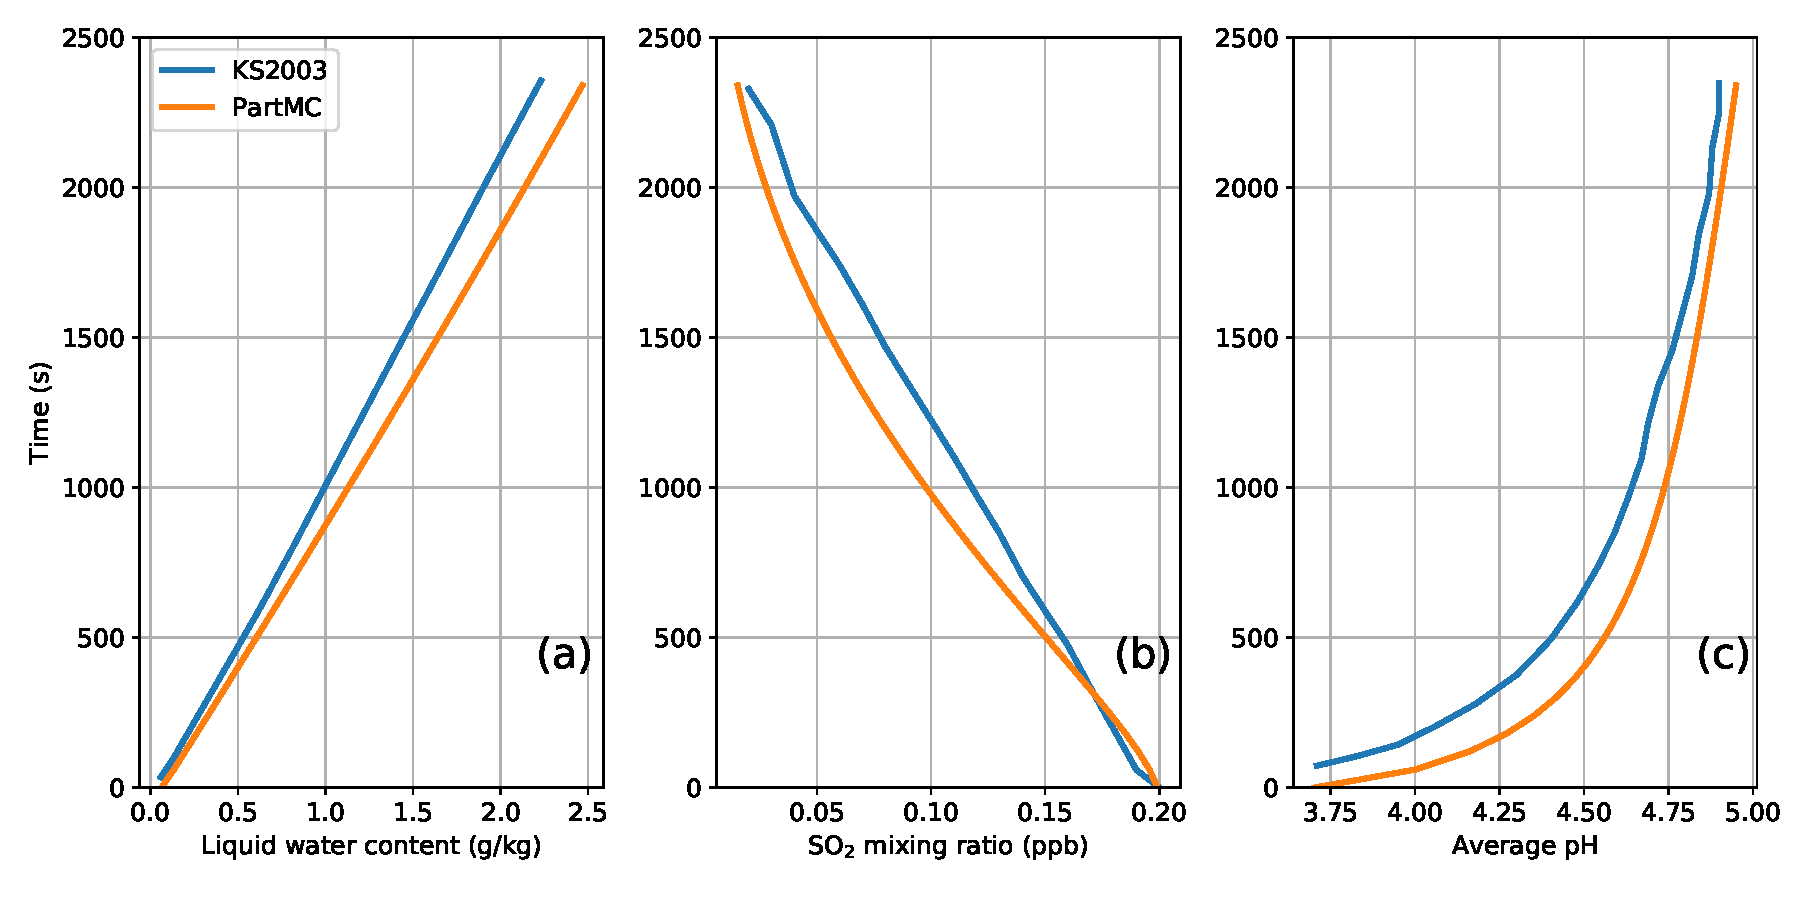
\includegraphics[scale=0.5]{chap2_figs/chap2_fig1_profile.pdf}
    \caption{Vertical profile differences of (a) liquid water content
      and (b) Gas $\rm SO_2$ concentration (c) Bulk pH between KS2003
      and PartMC.}
    \label{chap2:ks2003}
\end{figure}

The simulated decrease in $\rm SO_2$(g) mixing ratio is very similar
between PartMC and KS2003 (Fig.~\ref{chap2:ks2003}(b)), with $\rm
SO_2$(g) mixing ratio decreasing from 0.2 to 0.025~ppb after 40
minutes, indicating PartMC is capable of simulating of aqueous sulfate
formation processes. The bulk acidity calculated by PartMC also shows
similar profile with the models in KS2003 but with higher values
(Fig.~\ref{chap2:ks2003}(c)). Considering the different simulation
approaches, we expect some differences between bulk or size-binned
based pH and our particle-resolved pH.

Since the sulfate aqueous formation rate by $\rm O_3$ increases
exponentially with increasing pH, any differences in acidity
differences will propagate into sulfate production. At the end of the
simulation, PartMC simulated a sulfate mixing ratio of 207 ppb, higher
than the $\sim$175 in size-resolved models and $\sim$145 in bulk
models. As explained in KS2003, the excess produced sulfate in the
size-resolved models are found to be associated with higher simulated
pH and more sulfate formed from $\rm O_3$ oxidation pathway. This
explanation applies to our simulation results as well.

In summary, this comparison simulation proved our particle-resolved
aqueous model is capable of capturing the sulfate aqueous chemical
processes.  With more detailed particle information, our
particle-resolved approach may also provide more comprehensive
understanding of different sulfate formation pathways, and this is
explored in our next section.
%\begin{figure}
\section{Contribution of different aqueous sulfate formation pathways}
\label{chap2.4}
\subsection{Setup of idealized simulations using monodisperse aerosol}
To explore sensitivities of sulfate formation to the input parameters
(initial mixing ratios of selected gases and the cooling rate), I used
an idealized setup with monodisperse distributions for the initial
aerosol population. The purpose of these simulations is to confirm the
expected dependence of sulfate formation rates on pH and on the
presence of TMI.

The reference scenario ensemble exposed the monodisperse aerosol
populations to different initial conditions, denoted as $P_{\rm
  ref}$. The initial particle size was 100 \unit{nm}, composed of
ammonium sulfate. Emission of particle and gases and dilution with
background air were not included. The initial mixing ratios of $\rm
O_3$, $\rm H_2O_2$, $\rm NH_3$ and $\rm SO_2$, were perturbed at low,
medium and high polluted levels, as listed in
table~\ref{TMI-setting}. Gas phase $\rm SO_2$ was selected because it
provides the source of S(IV). The gas species $\rm O_3$ and $\rm
H_2O_2$ were selected because they are the important oxidants for
sulfate formation.  Ammonia also plays an important role in aqueous
sulfate formation by changing the droplet pH. The range of mixing
ratios for the different gas phase species are consistent with
observations in the ambient atmosphere. The $\rm O_3$ and $\rm SO_2$
values were based on the national-wide urban measurements in China
\citep{wang2014spatial}, and $\rm NH_3$ levels were determined from
the observations of Houston, U.S. \citep{nowak2010airborne} and Seoul,
Korea \citep{phan2013analysis}. The values for $\rm H_2O_2$ were based
on the measurements in Guangzhou, China
\citep{hua2008atmospheric}. The three different cooling rates provided
conditions with different liquid water content. The corresponded cloud
updraft velocity were 1.1, 1.5 and 1.8~\unit{m\;s^{-1}} respectively,
which represented the conditions of strong convective stratus
\citep{peng2005importance}. It is worth mentioned that updraft
velocities can change during the simulation period due to droplets
formation. A total of $3^5$ = 243 cases were run using all possible
combinations of input values to create this ensemble of scenarios.

\begin{table}[ht]
\centering
\caption{Settings for the initial conditions of the ensemble of
  scenarios denoted by $P_{\rm ref}$}
\label{TMI-setting}
\begin{tabular}{c  c c  c}
\hline
Parameters & Low  & Medium & High\\
\hline
$\rm O_3$& 25 & 50 & 75 \\
$\rm H_2O_2$& 0.25 & 0.5 &  1\\
$\rm NH_3$ &2 & 4 & 6 \\
$\rm SO_2$&2&5& 10\\
$\frac{dT}{dt}$ &$-$0.3 &$ -$0.4&$-$0.5\\
\hline
\end{tabular}
\end{table}

The initial RH was 99\% and each simulation time was 20~minutes. As
shown in Fig.~\ref{chap2:ensemrh}, cases with larger cooling rate
experienced more rapid increase of liquid water content, while the
maximum supersaturation was similar for all cases. Cloud droplets
formed in the first minute and the maximum supersaturation was 0.2\%.

\begin{figure}[ht]
    \centering 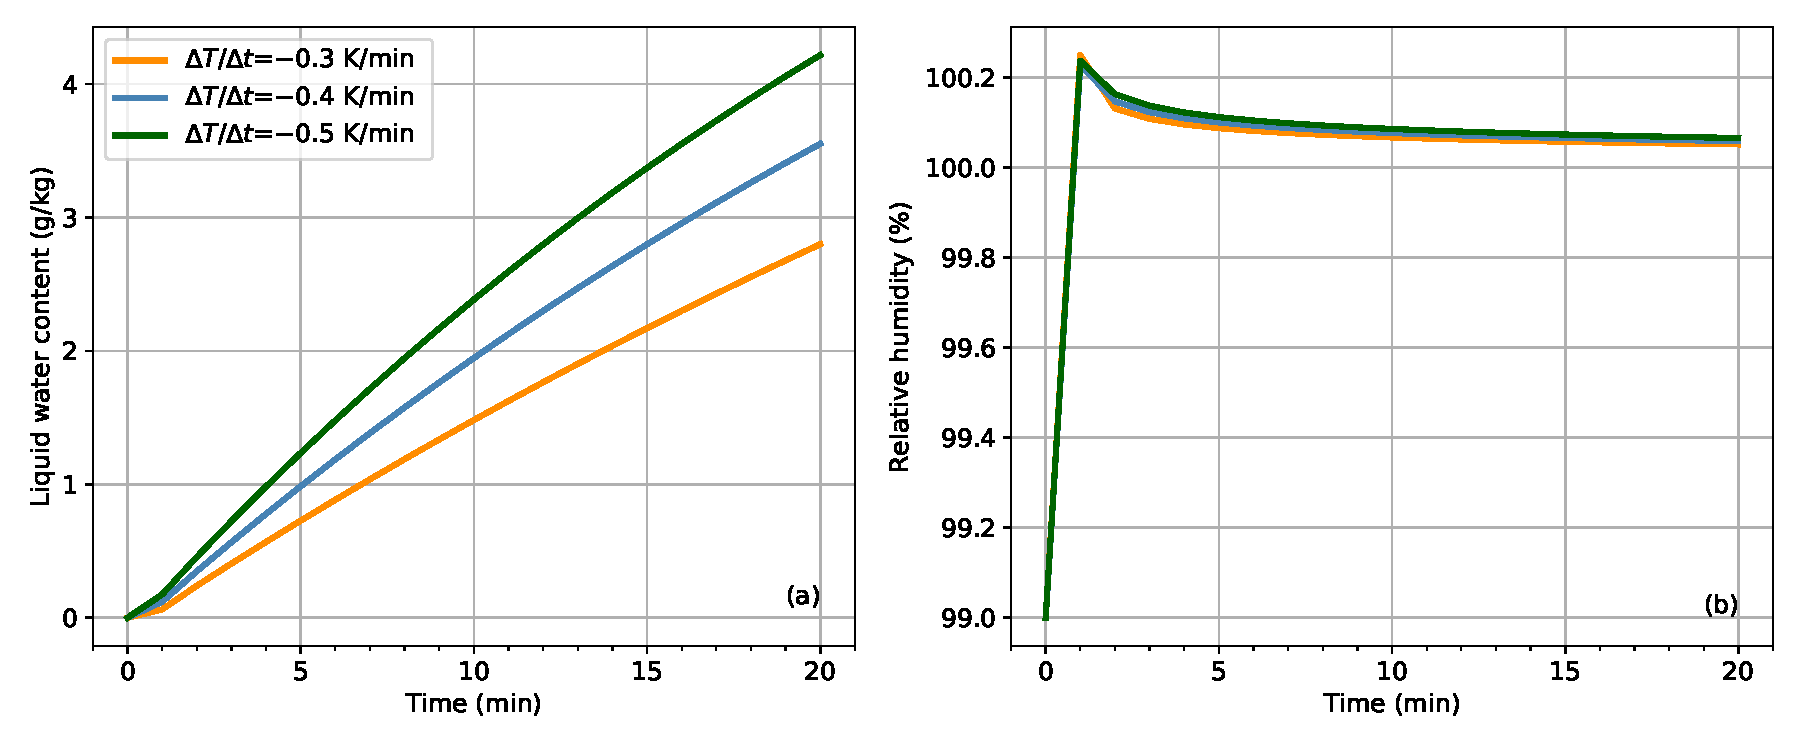
\includegraphics[scale=0.55]{chap2_figs/chap2_mono_lwc_rh.pdf}
    \caption{Time series of (a) liquid water content and (b) relative
      humidity in the ensemble of scenarios in $P_{\rm ref}$.}
    \label{chap2:ensemrh}
\end{figure}

To explore the sensitivity of sulfate formation to the presence of
TMI, another scenario ensemble was created, denoted as $P_{\rm TMI}$,
by adding $\rm Fe(II)$ and $\rm Fe(III)$ in the initial aerosol
population, with mass fractions of $\rm Fe(II)$ and $\rm Fe(III)$ to
be 0.05 and 0.01. We selected these two Fe mass fraction values to
produce Fe molar concentration consistent with previous studies
\citep{Deguillaume2005}.  Otherwise the setup was the same as for
$P_{\rm ref}$, which resulted in another 243 cases for $P_{\rm
  TMI}$. An important lesson of the $P_{\rm TMI}$ simulations was that
aqueous hydroxide needed to be present for TMI oxidation pathways to
proceed, with typical concentrations on the order of $\rm
10^{-13}$~\unit{M} \citep{deguillaume2004role}. Since OH was quickly
depleted in our initial setup, additional OH was supplied as emissions
at the rate of $2\times 10^{-8}$ \unit{mole/m^2/s} to maintain the
level of OH in the aqueous phase.

\subsection{Monodisperse aerosol simulation results}
This section explores the sensitivity of sulfate formation to selected
input parameters by analyzing the 243 aerosol populations in $P_{\rm
  ref}$.  Figure~\ref{chap2:ens_three} shows the sulfate mixing ratio
for all scenarios, stratified by the five different input parameters,
including $\rm NH_3$, $\rm H_2O_2$, $\rm O_3$, $\rm SO_2$, and the
temperature lapse rate.

A clear separation exists between the cases with different initial
ammonia gas mixing ratio, where higher sulfate production is
associated with higher initial ammonia mixing ratio. However, this
separation is not as clear for the other four parameters. This
reflects the fact that the sulfate production rates change over time
within the cloud droplets as the concentrations of aqueous-phase
species involved in sulfate production also change. While the initial
conditions of $\rm H_2O_2$ and $\rm O_3$ play some role, they do not
entirely determine the outcome. Cases with higher sulfate formation
(the blue curves in Figure~\ref{chap2:ens_three}a) are seen with all
levels of temperature lapse rate, $\rm H_2O_2(g)$ and $\rm O_3(g)$
mixing ratio. However, the highest sulfate mixing ratios are
associated with high initial $\rm O_3$ and $\rm SO_2$ mixing
ratios. This phenomenon indicates that the ammonia gas phase mixing
ratio is a determining factor for aqueous sulfate formation in the
simulated scenarios under consideration. Next, we will look into the
underlying mechanism.
%It is
%worth mention that we currently analyzed the sulfate production rates
%by connecting with the initial gas mixing ratios. However, aqueous
%%sulfate formation rates depend on what is actually in the aqueous
%phase and it changes with time.

\begin{figure}[ht]
    \centering 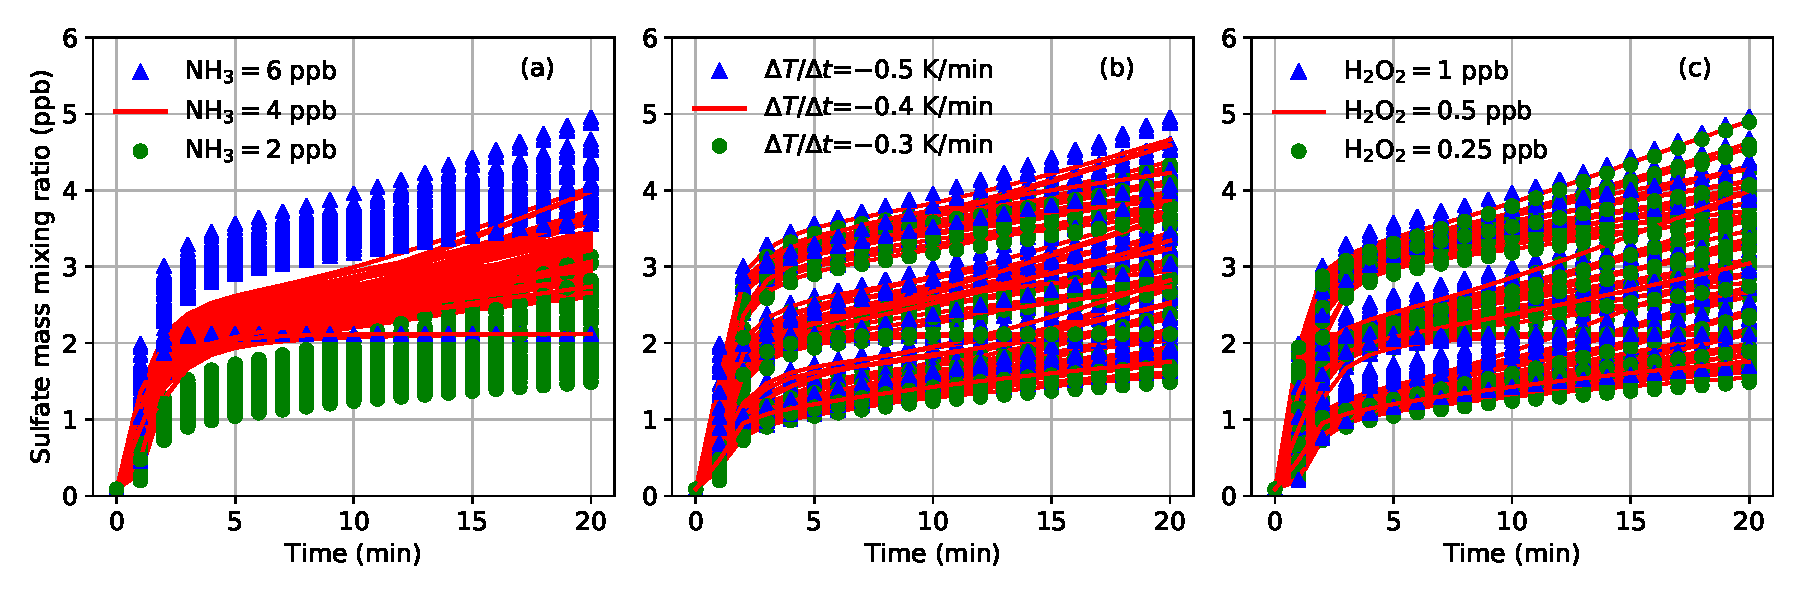
\includegraphics[scale=0.55]{chap2_figs/chap2_fig2_mono_ensemble.pdf}
    \caption{Sulfate time series categorized by five different
      settings in $P_{\rm ref}$: (a) initial $\rm NH_3(g)$ mixing
      ratio, (b) temperature lapse rate, (c) initial $\rm H_2O_2(g)$
      mixing ratio, (d) initial $\rm O_3(g)$ mixing ratio, and (e)
      initial $\rm SO_2(g)$ mixing ratio. The three colors and symbols
      are for the low, medium and high levels of each parameter.}
    \label{chap2:ens_three}
\end{figure}

Gas $\rm SO_2$ is highly soluble to water and it dissolves
rapidly. The dissolved $\rm SO_2$ in the cloud droplets can appear in
three S(IV) forms: $\rm SO_2\cdot H_2O$, $\rm HSO_3^-$ and $\rm
SO_3^{2-}$. S(IV) is then oxidized to S(VI) (sulfate). Here, I
analyzed four key oxidation pathways which transfer the S(IV) species
to S(VI):
\begin{align}
\centering
    &\ce{HSO3^- + H2O2{(aq)} + H^+ -> SO4^{2-} + 2H^+ + [H2O](aq)}\\
    &\ce{HSO3^- + O3{(aq)} -> SO4^{2-} + H^+ + O2{(aq)}} \\
    &\ce{SO3^{2-} + O3{(aq)} -> SO4^{2-} + O2{(aq)}} \\
    \label{eq:chem-eq}
    &\ce{S(IV) + \frac{1}{2}O2 ->[TMI] S(VI)}
\end{align}
This section will focus on the discussion of the first three oxidation
pathways and transition pathway reaction~\ref{eq:chem-eq} will be
discussed in next section.

Figure~\ref{chap2:su-acidity} shows the relationship between sulfate
mixing ratio and particle acidity at 3~\unit{min}. For the cases with
the same initial $\rm SO_2(g)$, the sulfate mixing ratio is higher for
higher initial $\rm NH_3(g)$. Considering the cases with $\rm SO_2(g)$
of 5~\unit{ppb} and $\rm O_3(g)$ of 50~\unit{ppb} (the cases in the
red boxes of Fig~\ref{chap2:su-acidity}), the only differences for
these cases are the initial $\rm NH_3(g)$ values. For all three
cooling rates, when $\rm NH_3(g)$ increased from 2 to 6~\unit{ppb}, pH
increased from 5.0 to over 5.5 and sulfate mixing ratio increased from
1~\unit{ppb} to more than 2.5~\unit{ppb}. This is because the reaction
rates of the $\rm O_3$ pathways increase for higher pH
(Fig.~\ref{chap2:reac-rates}). Fig.~\ref{chap2:reac-rates} also shows
that for cases with 10~\unit{ppb} $\rm SO_2$, $\rm H_2O_2$ reaction
rates are almost constant at all $\rm NH_3$ levels. The different
responses of $\rm O_3$ and $\rm H_2O_2$ pathways are consistent with
the descriptions in \citet{Seinfeld2016}. For $\rm O_3$ pathways, high
pH leads to high S(IV) solubility and reaction rates increased (the
cases in the red boxes of Fig~\ref{chap2:reac-rates}). The reactions
are self-limiting because the produced sulfate will increase acidity
and decrease pH. In contrast, the $\rm H_2O_2$ pathway is insensitive
to pH because of the canceling effects between increased S(IV)
concentration and reduced reaction constants. For the cases with
2~\unit{ppb} initial $\rm SO_2$, the reaction rates are smaller for
the cases with higher $\rm NH_3$ and pH. These are $\rm
SO_2(g)$-limited cases and less dissolved $\rm SO_2$ is responsible
for this.

\begin{figure}[ht]
    \centering 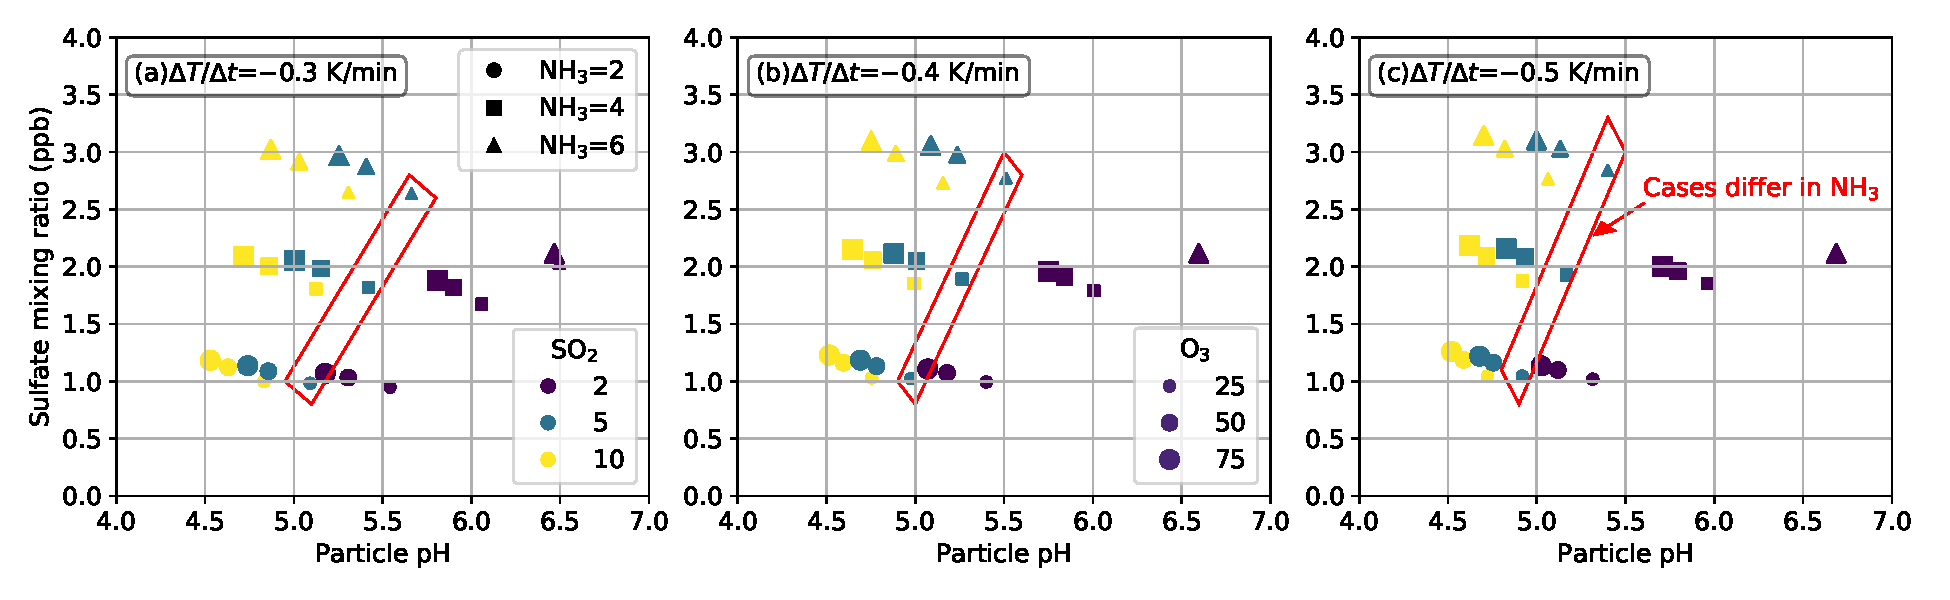
\includegraphics[scale=0.53]{chap2_figs/chap2_fig4_sulfate_pH_3min.pdf}
    \caption{Correlation between sulfate mixing ratio and acidity at
      3~\unit{min}. (a) is for cases with temperature lapse rate of
      $-0.3$~\unit{K/min}. (b) is for cases with temperature lapse
      rate of $-0.4$~\unit{K/min}. (c) is for cases with temperature
      lapse rate of $-0.5$~\unit{K/min}. Symbols in the plots are
      colored by $\rm SO_2$(g) levels and symbol types are for $\rm
      NH_3$(g) levels. All the cases in the figure are with $\rm
      H_2O_2(g)$ = 0.5~\unit{ppb}. Red boxes are for the aerosol
      populations with only differences in $\rm NH_3(g)$ and are
      analyzed for detail in the text.}
    \label{chap2:su-acidity}
\end{figure}

As for the sensitivity to temperature, there is no significant
differences for cases with different cooling rates
(Fig~\ref{chap2:reac-rates}). As \citet{Seinfeld2016} described, the
effects of temperature on reaction rates are the balancing effects
between two factors. On the hand, lower temperature leads to higher
solubility and higher reactions rates. On the other hand, reaction
constants decrease with lower temperature. Thus, when temperature
changes, the behaviour of reactions rates are determined by which
factor is dominant. 

\begin{figure}[ht]
    \centering 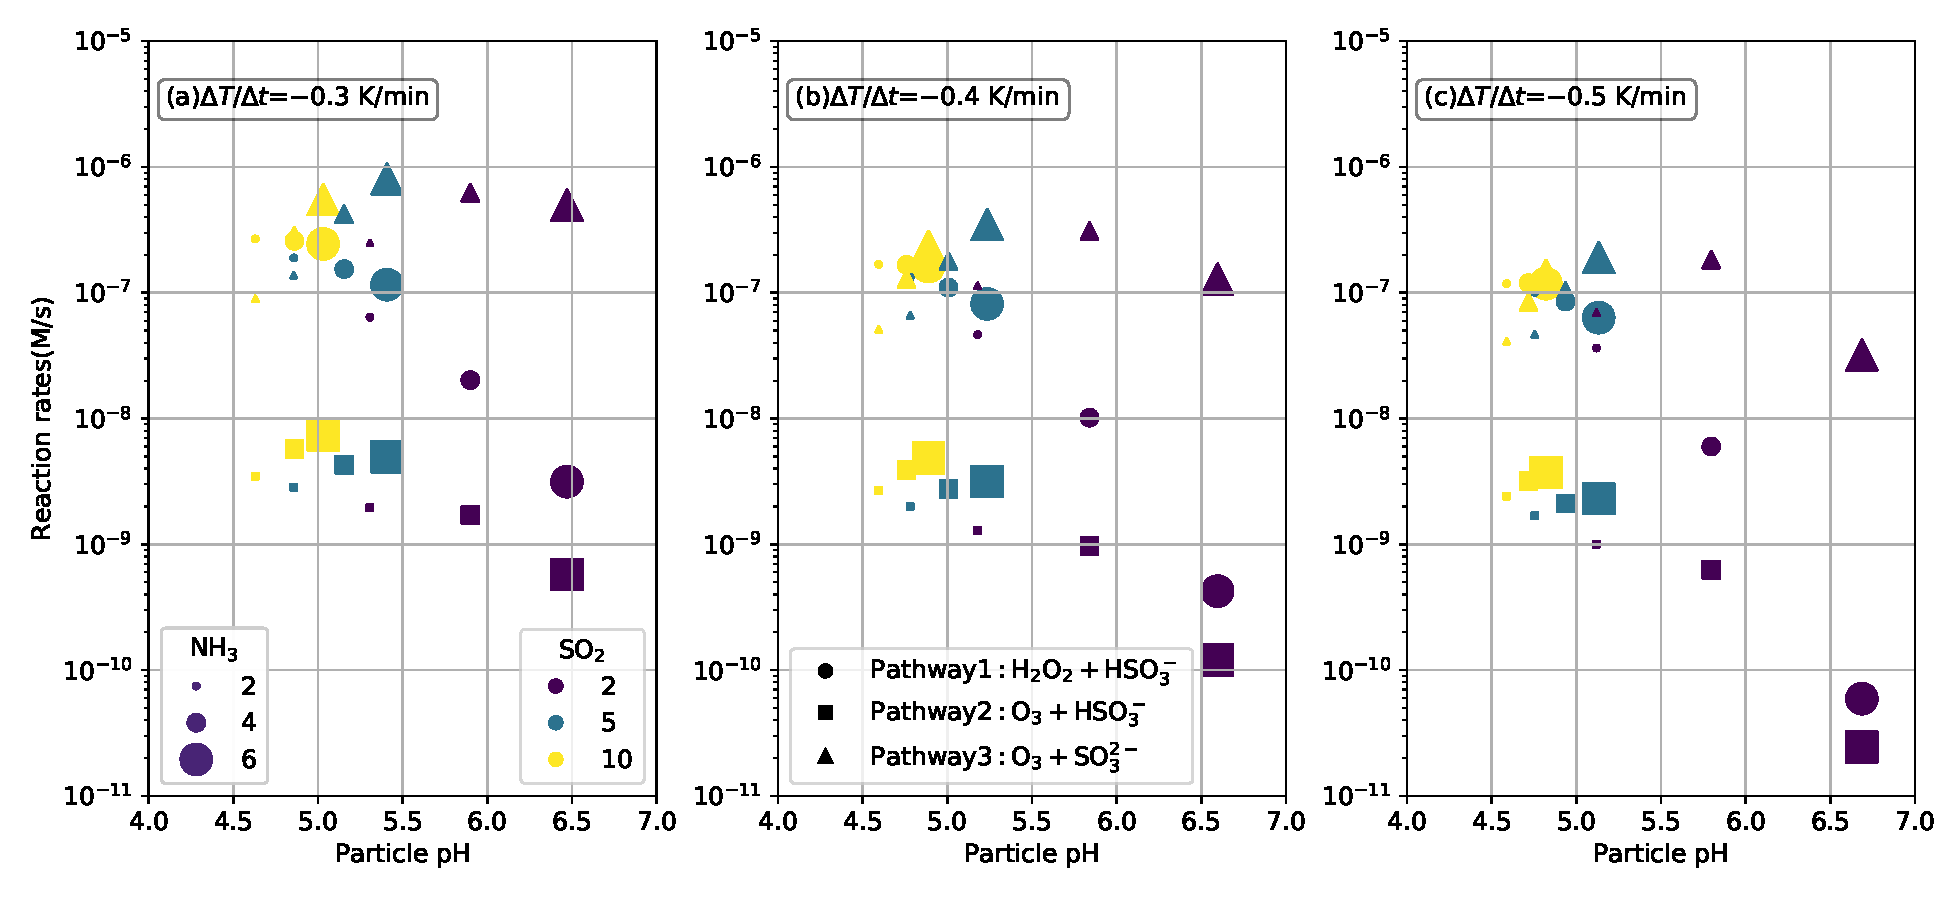
\includegraphics[scale=0.53]{chap2_figs/chap2_fig6_sulfate_pH.pdf}
    \caption{Relationship between aqueous sulfate formation rates and
      particle acidity at $t=3$~min. (a) temperature lapse rate of
      $-0.3$~\unit{K/min}. (b) temperature lapse rate of
      $-0.4$~\unit{K/min}. (c) temperature lapse rate of
      $-0.5$~\unit{K/min}. Symbol types are for different oxidation
      pathways: circle is for $\rm H_2O_2+ HSO_3^-$, square is for
      $\rm O_3+ HSO_3^-$ and triangle is for $\rm O_3+
      SO_3^{2-}$. Color is for $\rm SO_2(g)$ level and symbol size
      represents $\rm NH_3(g)$ level. All the cases in the figure are
      with $\rm O_3(g) = 50$~\unit{ppb} and $\rm H_2O_2(g) =
      0.5$~\unit{ppb}. Red boxes are for the aerosol populations with
      only differences in $\rm NH_3(g)$ and are analyzed in more
      detail in the text.}
    \label{chap2:reac-rates}
\end{figure}

%Detail statistics of the three pathways are further explored in
%Fig.~\ref{chap2:reac-rates}. Sulfate formation through $\rm H_2O_2+
%HSO_3^-$ and $\rm O_3(aq)+ SO_3^{2-}$ pathways are 1--2 orders higher
%than $\rm O_3(aq) + HSO_3^-$. The higher rates of $\rm O_3+
%SO_3^{2-}$ than $\rm O_3+ HSO_3^{-}$ can be explained by the
%different nucleophilic reactivity. The oxidation rates of $\rm
%HSO_3^-$ by $\rm H_2O_2(aq)$ and $\rm O_3(aq)$ increase rapidly with
%increasing $\rm SO_2$(g) mixing ratio. For the cases with
%6~\unit{ppb} $\rm NH_3$(g), median reaction rates of $\rm H_2O_2(aq)
%+ HSO_3^-$ jump from $10^{-9}$~\unit{M/s} at 2~\unit{ppb} $\rm
%SO_2$(g) to $10^{-7}$~\unit{M/s} at 10~\unit{ppb} $\rm SO_2$(g). But
%for oxidation of $\rm SO_3^{2-}$ by $\rm O_3(aq)$, the reaction rate
%and $\rm SO_2$(g) mixing ratio is negative correlated. That can
%explain why there is no strong correlation between $\rm SO_2$(g)
%mixing ratio and high sulfate formation rates. As for $\rm NH_3$(g),
%oxidation rates of $\rm HSO_3^-$ and $\rm SO_3^{2-}$ by $\rm O_3(aq)$
%is higher at the cases with 6~\unit{ppb} $\rm NH_3$(g), and there is
%no clear change for $\rm H_2O_2(aq) + HSO_3^-$ at different $\rm
%NH_3$ levels. This is consistent with what we found the most sulfate
%formation cases are connected with high $\rm NH_3(g)$ cases. The only
%anomalous cases are for the aerosol populations with 2~\unit{ppb}
%$\rm NH_3(g)$, where the reaction rates decreased with increasing
%$\rm NH_3(g)$. This is the $\rm SO_2(g)$-limited cases we mentioned
%above.

%\begin{figure}[ht] \centering
%    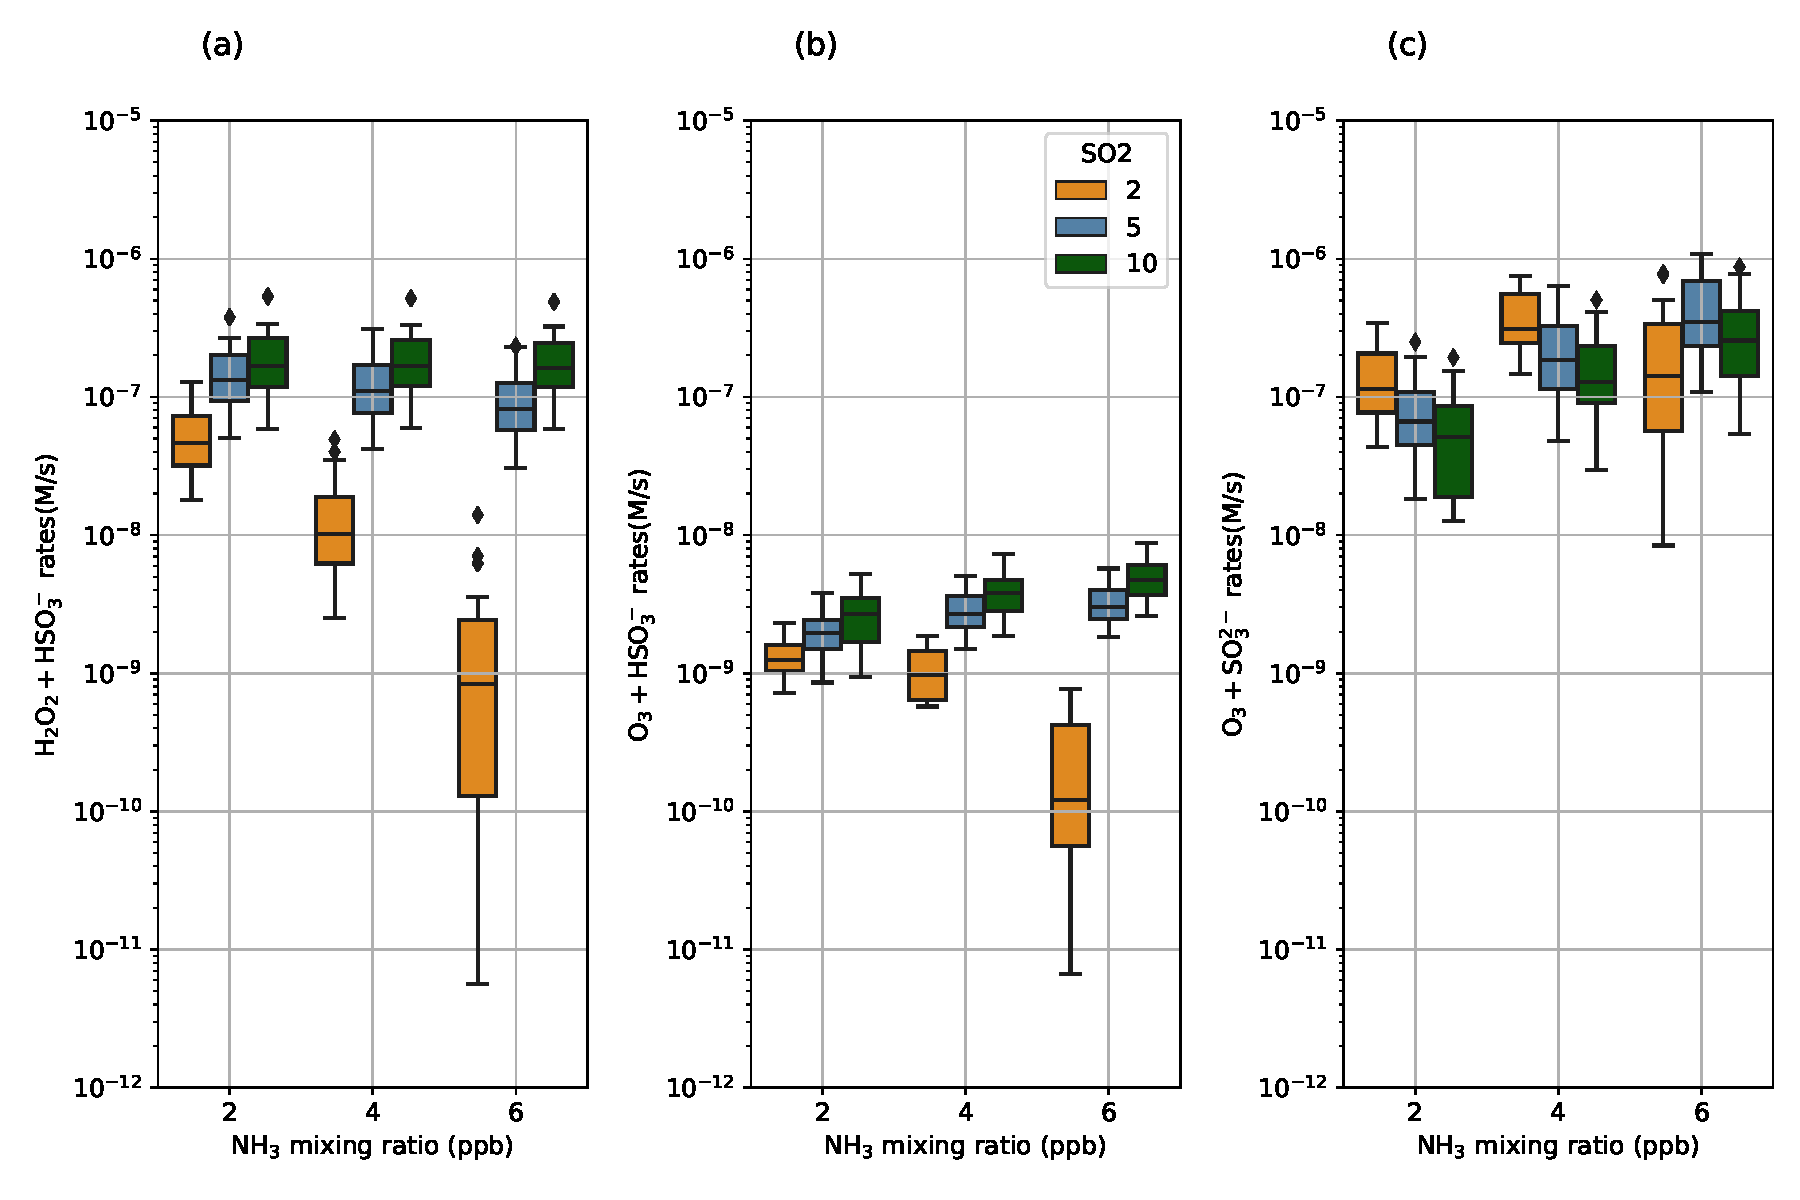
\includegraphics[scale=0.55]{chap2_figs/chap2_fig5_sulfate_rates_3min.pdf} \caption{Statistics
%    of three aqueous sulfate formation pathway rates:$\rm H_2O_2$ +
%    $\rm HSO_3^-$(a), $\rm O_3$ + $\rm HSO_3^-$(b), $\rm O_3$ + $\rm
%    SO_3^{2-}$. Cases are grouped by $\rm NH_3(g)$ and $\rm
%    SO_2$.}  \label{chap2:rates-stats} \end{figure}

Based on analysis for the cases in $P_{\rm ref}$, we can conclude that
the aqueous sulfate formation is most sensitive to the initial $\rm
SO_2(g)$ and initial $\rm NH_3(g)$ mixing ratios. Cases with most
sulfate formation were for the cases with high $\rm NH_3(g)$ values
and this can be explained by the higher oxidation rates of $\rm
SO_3^{2-}$ by $\rm O_3(aq)$. Cases with higher $\rm NH_3(g)$ but lower
sulfate production were because of a lower supply of $\rm SO_2(g)$,
making sulfate formation was $\rm SO_2(g)$-limited. Overall, our
particle-resolved aqueous chemistry model is capable of simulating the
expected response of $\rm O_3$ and $\rm H_2O_2$ pathways to
temperature and acidity changes.

\section{Contribution of TMI pathways to sulfate formation} 
\label{chap2.5}
This section presents the 243 cases containing iron components in
$P_{\rm TMI}$ and explore the contributions of TMI catalyzed
reactions. Figure~\ref{chap2:iron-conc}(a) shows the time series of
$\rm Fe^{2+}$, $\rm Fe^{3+}$ and OH(aq) median molar concentration.

$\rm Fe^{2+}$ varies between $10^{-11}$ and $10^{-7}$ and $\rm
Fe^{3+}$ ranges between $10^{-7}$ and $10^{-6}$~\unit{M}, both are in
the same order with the values in \citet{Deguillaume2005}. By adding
TMI, the median sulfate mixing ratio in $P_{\rm TMI}$ significantly
increased from 2~\unit{ppb} to
5~\unit{ppb}. Figure~\ref{chap2:iron-contri} further explores the
contribution ratio changes of different aqueous sulfate pathways after
adding TMI to the population.

\begin{figure}[ht]
    \centering 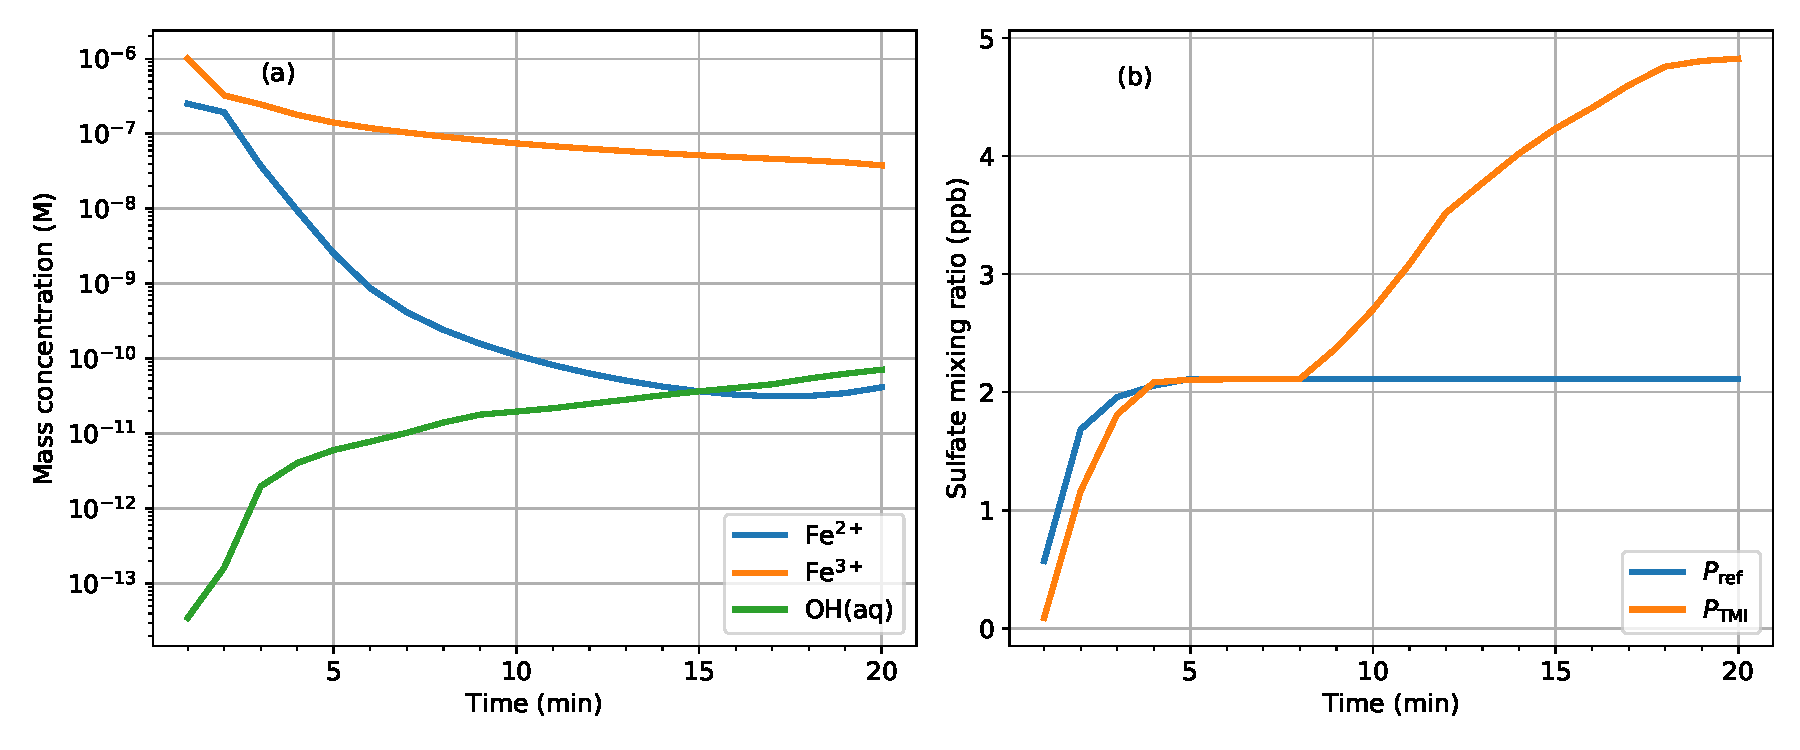
\includegraphics[scale=0.53]{chap2_figs/chap2_with_tmi_fixOH_mass.pdf}
    \caption{Time series of (a) $\rm Fe^{2+}$, $\rm Fe^{3+}$ and $\rm
      OH(aq)$ (b) Sulfate mixing ratio in $P_{\rm ref}$ and $P_{\rm
        TMI}$. Values are the median of all the cases in the ensemble
      $P_{\rm TMI}$. }
    \label{chap2:iron-conc}
\end{figure}

Oxidation of $\rm HSO_3^-$ by $\rm O_3$ and $\rm H_2O_2$ are the
dominant pathways for aqueous sulfate formation in $P_{\rm ref}$
(Fig.~\ref{chap2:iron-contri}(a)). These two pathways in total
contributed to more than 90\% of sulfate formation over the simulation
period, and there is no contribution of TMI
pathways. But in $P_{\rm TMI}$, these two pathways are dominant at the
first 2 minutes and sulfate formation through the reaction between
$\rm SO_4^-$ and water is dominant afterwards
(Fig.~\ref{chap2:iron-contri}(b)). I also noticed a remarkable
contribution from TMI pathway after 4~\unit{min}, and the contribution
ratio can be more than 20\% at the end of simulation.

\begin{figure}[ht]
    \centering
    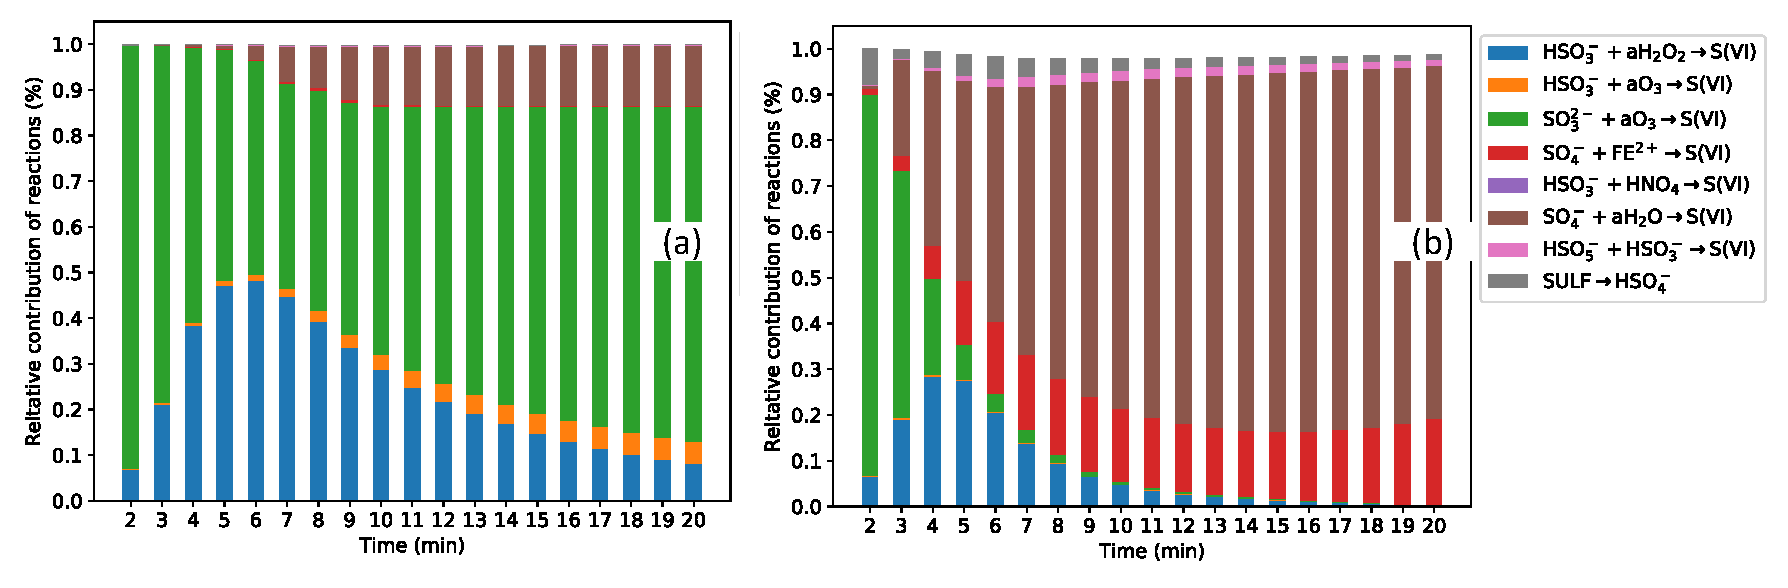
\includegraphics[scale=0.57]{chap2_figs/chap2-TMI_contri_factors.pdf}
    \caption{Mean contribution fraction of different sulfate formation
      pathways in (a)$P_{\rm ref}$ and (b)$P_{\rm TMI}$}
    \label{chap2:iron-contri}
\end{figure}

It is worth a reminder that OH(g) was emitted at a constant rate for
the cases $P_{\rm TMI}$, while there was no emission of OH(g) in
$P_{\rm ref}$. Based on current simulation settings, we can not
distinguish the role of OH and TMI for the increased sulfate
production rates in $P_{\rm TMI}$.  However, we can still learn from
the current result is conditions exist where sulfate formation through
TMI pathways can be important, and PartMC is able to capture this.

\section{Conclusion}
\label{chap2.6}
For the work presented in this chapter, we used the particle-resolved
model PartMC as cloud parcel model with a comprehensive aqueous
chemistry module CAPRAM2.4 to investigate the role of different
aqueous sulfate formation pathways. The model was evaluated using
results from size-resolved and bulk aqueous models from the
literature, and our model reproduced similar $\rm SO_2$(g) and acidity
profiles.

We designed an ensemble of scenarios to investigate the response of
sulfate formation to varying input parameters. As expected, cases with
high $\rm NH_3(g)$ and $\rm SO_2(g)$ produced the most sulfate. This
can be explained by efficient oxidizing reactions between $\rm
SO_3^{2-}$ and $\rm O_3(aq)$ because of the higher pH that exists when
$\rm NH_3(g)$ is supplied. Our particle-resolved aqueous chemistry
model reproduces the expected responses of $\rm O_3$ and $\rm H_2O_2$
pathways to pH. Analysis of another ensemble scenario with TMI present
shows S(IV) reactions catalyzed by TMI can contribute up to 20\% of
the sulfate production, and the fraction was consistent with the
values found by \citet{alexander2009transition}.

%%%Future work%%%
The representation of TMI oxidation processes is rather simple in this
current setup. Iron from different sources has different solubility
\citep{desboeufs2005dissolution}. It would be therefore be better to
connect the soluble fraction of iron to its sources to investigate the
conditions most favorable for TMI-catalyzed reactions more
realistically. Further, the need for ``OH emissions'' is an artefact
of not having entrainment or gas-phase chemistry ocurring when aqueous
phase chemistry is simulated. If we had entrainment, then fresh OH any
be supplied from outside the cloud, and similarly, if we had gas-phase
chemistry enabled, OH may be produced in the gas phase and could
partition with the aqueous phase. In future model development, both
processes should be considered to be included.

%%%%%%%%%%%%%%%%%%%%%%%%%%%%%
%%%%%%%%%Chapter 3%%%%%%%%%%%
%%%%%%%%%%%%%%%%%%%%%%%%%%%%%
\chapter{Evaluating the impacts of cloud processing on resuspended aerosol particles after cloud evaporation using a particle-resolved model}

This chapter quantifies the changes of aerosol properties after cloud
processing using the particle-resolved aqueous chemistry model. First
I introduce model details, mixing state metrics and cloud parcel
simulation design. Then, I present the changes in number and mass
distribution changes after cloud processing. Finally, I discuss the
changes in aerosol mixing state, CCN concentration and aerosol optical
properties after cloud processing. The first part about cloud
processing effects on aerosol mixing state is currently under review
with \textit{Journal of Geophysical Research-Atmosphere}, and the
second part about the changes in aerosol optical values is in
preparation for \textit{Aerosol Science and Technology}.
  
\label{chap3}
\section{Introduction}
Atmospheric aerosol particles are complex mixtures of different
chemical species reflecting the fact that they originate from
different emission sources and experience various aging processes in
the atmosphere \citep{Riemer2009, Li2011a, Bondy2018, Healy2014,
  Rissler2014}.  Aging processes include processes in the cloud-free
atmosphere such as coagulation, heterogeneous reactions on the
particles' surface, and the formation of coatings from organic and
inorganic secondary aerosol. They also include processes in clouds
\citep{Lance2017} such as aqueous-phase chemistry within cloud droplets
forming inorganic and organic aerosol material, and
collision-coalescence of particles and droplets within a cloud. When
clouds evaporate, aerosol populations are released into the atmosphere
with modified properties compared to the populations that formed the
cloud. This, in turn, changes the aerosols' impacts on clouds in the
next cloud cycle \citep{Hoose2008}, and therefore this process is
important for 3D chemical transport models to include. At the same
time it poses challenges to be represented in chemical transport
models \citep{Gao2016}.

Specifically, in-cloud processes have been shown to produce a double
peaked size distributions since material from the gas phase and from
smaller particles is transferred to the accumulation mode size range
\citep{Hoppel1986,Noble2019}. It has also been observed that cloud
droplets of different sizes may differ in their acidity
\citep{Collett1994,Pye2020}. This has important implications for the
rates of aqueous-phase sulfate formation \citep{Hoag1999}, which
depends strongly on pH, and this needs to be considered when
representing these processes in cloud microphysics models
\citep{Hegg1990,Barth2006}. Because of the non-linearity of aqueous
chemistry processes, models predict larger rates of sulfate formation
when using a more realistic size-resolved droplet representation
compared to using a prescribed single droplet size.

In this study, we not only considered the variation of aerosol (and
cloud droplet) composition with size, but also the variation of
composition within a narrow size range, commonly referred to as mixing
state \citep{Winkler1973,Riemer2019}. Our goal in this study was to
quantify the changes in aerosol mixing state due to in-cloud 
aqueous-phase chemistry and coagulation processes. Aerosol mixing state
impacts the aerosols' effects on health \citep{Ching2018}, their
absorption and scattering of sunlight \citep{Lesins2002,Fierce2020},
and their ability to act as cloud condensation and ice nuclei
\citep{Broekhuizen2006,Bhattu2015,Knopf2018}.

Mixing state is, on the one hand, a factor in determining which
particles activate and form cloud droplets, thereby determining cloud
properties \citep{ching2012impacts,Ching2016}. On the other hand,
mixing state can be modified by in-cloud processes. For example,
observations using online single-particle mass spectrometry during the
HCCT-2010 field campaign showed that cloud residuals contain more
sulfate and nitrate compared to the below-cloud aerosol
\citep{Roth2016}, resulting in a change of aerosol mixing state.

Model simulations of aerosol mixing state are challenging, and
particularly rare when it comes to simulating in-cloud processes due
to the need for extensive computing resources.  Regional or global
models use simplified assumptions about aerosol activation and aerosol
mass and size changes due to cloud processing, which are determined by
the underlying model representation of aerosol and cloud droplets. For
example, in the CMAQ model, which uses a modal aerosol representation,
the sulfate mass produced by in-cloud chemistry is added to the entire
accumulation mode \citep{Ervens2015, Fahey2017}. In the global
  climate model ECHAM5-HAM, activated particles are grouped into two
  bins, one with low ion concentration and the other with higher ion
  concentration \citep{roelofs2006aerosol} to capture the dependence of
  the sulfate formation pathway on pH.

High-resolution cloud models typically use a size-resolved fixed-bin
microphysical model \citep{Flossmann1994,Feingold1996} and resolve
aerosol particles and cloud droplets by separate distributions, thus
internally mixing all same-sized particles or droplets. Similarly,
accurate parcel models most frequently use a size-resolved moving-bin
approach \citep{Kreidenweis2003,Cooper1997}, again losing aerosol
history and composition information within each size bin. To preserve
some composition information, 2D aerosol models have been used,
resolving cloud droplet size and aerosol dry volume
\citep{Bott1996,Ovchinnikov2010}. However, increasing the dimension
beyond 2D to treat composition variation of the aerosol in more detail
would be computationally prohibitively expensive. Lagrangian cloud
microphysics models have also been developed that track
information on a droplet level \citep{Shima2009,
  Andrejczuk2008,Grabowski2019,Soelch2010,
  Unterstrasser2014,Jaruga2018}. However, their focus has been the
study of cloud microphysics rather than the modification of aerosol
composition. While \citet{Jaruga2018} consider some aqueous-phase
chemistry processes, their representation of the aerosol is
comparatively simple and questions about mixing state have not yet
been addressed.

For our study, we used the aerosol model PartMC-MOSAIC (Particle Monte
Carlo-Model for Simulating Aerosol Interactions and Chemistry)
\citep{Riemer2009,Zaveri2008} as aerosol and cloud parcel model. This
stochastic particle-resolved model explicitly resolves the composition
of individual aerosol particles and cloud droplets in a given
population. Since individual particles and droplets are explicitly
tracked, there is no need to invoke ad hoc aging criteria that move
aerosol mass between bins or modes as is the case with traditional
modal or sectional approaches \citep{Riemer2003,Stier2005,
  Bauer2008,Jacobson2001}. Tracking droplets explicitely is therefore
a well-suited to simulate aerosol mixing state and investigate its
impacts on climate-relevant aerosol properties.

The model was described in \citet{ching2012impacts} and \citet{Ching2016} and
has been used to simulate the mixing state evolution of
black-carbon-containing aerosol in the cloud-free atmosphere, followed
by a process analysis to what extent the aged aerosol is able to
undergo nucleation-scavenging as the particles compete for water vapor
in an updraft. However, these studies did not include the effects of
aqueous-phase chemistry ocurring within the cloud droplets. This is
the motivation for this study, where we extended our modeling framework
to include aqueous-phase chemistry within the cloud droplets that are
forming on a diverse population of particles, common to urban
environments. The contribution of this chapter is the first study to
document quantitatively the impact of aqueous phase
chemistry on mixing state.

We focused on the following questions: (1) To what extent does cloud
processing change the aerosol mixing state of the population that
entered the cloud? (2) How does this change the cloud condensation
number concentration and aerosol optical properties? (3) What
is the role of coagulation between the interstitial particles and
cloud droplets for mixing state of the aerosol?

Chapter~\ref{sec:model} describes the model components, the scenario
setup, and the mixing state metrics used in this
study. Chapter~\ref{sec:results} presents the analysis of the
simulation results. Chapter~\ref{sec:conclusions} summarizes our
results.
%

\section{Model description and metrics}
\label{sec:model}
\subsection{Stochastic particle-resolved module PartMC-MOSAIC}
Aerosol physical and chemical processes were simulated by the
stochastic particle-resolved model PartMC-MOSAIC (Particle Monte
Carlo-Model for Simulating Aerosol Interactions and Chemistry-Model
for Simulating Aerosol Interactions and Chemistry, \citep{Riemer2009,
  Zaveri2008}). The PartMC model simulates the evolution of
per-particle composition of a large ensemble of computational
particles in a well-mixed computational volume. In contrast to
Lagrangian droplet models that have become popular in the cloud
microphysics community \citep{Shima2009,Grabowski2019}, PartMC-MOSAIC
does not track the position of particles and droplets within the
computational volume.

The particle number concentration changes due to coagulation, emission
and dilution, which are simulated by using a stochastic Monte Carlo
sampling method \citep{Riemer2009}. Gas-phase chemistry and
gas-particle partitioning are represented by the aerosol chemistry
model MOSAIC, which includes CBM-Z for gas-phase photochemical
reactions \citep{Zaveri1999}, MTEM for estimating mean activity
coefficient of an electrolyte in a inorganic multicomponent solution
\citep{Zaveri2005} and MESA for intraparticle solid-liquid
partitioning for inorganic aerosols \citep{Zaveri2005a}. The formation
mechansim of secondary organic aerosol (SOA) in MOSAIC is based on
SORGAM \citep{Schell2001} with several parameters adjusted to bring the
simulated values closer to observation \citep{Zaveri2010a}. The model
represents key aerosol species including sulfate, nitrate, ammonium,
black carbon (BC), primary organic aerosol (POA) and several surrogate
secondary organic aerosol (SOA) species. The coupled model
PartMC-MOSAIC was applied in previous studies for simulating aerosol
optical and CCN properties, black carbon aging time-scales and the
black carbon absorption enhancement due to the coatings
\citep{Zaveri2010a, Riemer2010, Fierce2017,Fierce2020}, focusing on
mixing state evolution during cloud-free conditions. The model was
also used for evaluating the impact of aerosol mixing state on cloud
droplet formation \citep{ching2012impacts,Ching2016}, which will be explained
in more detail in the next section.

\subsection{Cloud parcel model and aqueous-phase chemistry}
\citet{ching2012impacts} described the details of the particle-resolved cloud
parcel model, which simulates a population of aerosol particles that
experience cooling at a prescribed cooling rate and subsequent growth
due to the condensation of water vapor. The condensational growth of
the particles is calculated following \citet{Seinfeld2016}. The
driving force of the growth is the difference between droplet
equilibrium saturation vapor pressure and the ambient vapor pressure
of the environment. The equilibrium saturation vapor pressure is
calculated by K\"ohler theory, and the particle hygroscopicity is
determined using the parameterization of aerosol hygroscopicity
developed by \citet{Petters2007}. The hygroscopicity $\kappa$
  of each particle is calculated by using the volume-weighted average
  of the individual $\kappa$ values of the particles' constituent
  species. We used $\kappa$ of 0.65 for ammonium sulfate and ammonium nitrate,
  $\kappa$ of 0.1 for SOA and $\kappa$ of 0.001 for POA.  BC is
  assumed to be hyrophobic and had $\kappa$ of 0.  The hygroscopicity
  of each particle varied as the chemical composition evolved for each
  particle. We currently do not represent any entrainment of
cloud-free air into the cloud, surface tension effects on droplet
growth, or the loss of droplets from the air parcel owing to
sedimentation.

The aim of this chapter is to investigate impacts of in-cloud
aqueous-phase chemistry on aerosol mixing state. To this end, we
coupled the reduced Chemical Aqueous Phase Radical Mechanism (CAPRAM)
2.4 to PartMC-MOSAIC. The reduced CAPRAM model includes 183 reactions
(including Henry's Law partitioning, dissociation reactions,
photolysis reactions and other aqueous-phase reactions) and 113
species \citep{Herrmann1999, ervens2003capram}. The mechanism
treats the reactions of common radicals and radical anions, transition
metal ions and organics with less than two carbon atoms. The CAPRAM
mechanism was applied to simulate the cloud processes for the FEBUKO
field campaign and reproduced the aqueous sulfate and organic
compounds oxidation processes well \citep{Tilgner2005, Wolke2005}.
While the aqueous-phase chemistry involving transition metal ions and
organic species is of great interest
\citep{Mayol-Bracero2002,Harris2013a, Alexander2009, Lian2019,
    McNeill2015a, Smith2014, wonaschuetz2012aerosol,wagner2015situ},
our scope for this initial study is the in-cloud production of
  sulfate and nitrate and their relationship to changes in aerosol
  mixing state. We did not consider the co-condensation of nitric acid
  gas due to vapor pressure difference discussed by
  \citet{crooks2018parameterisation}. A subset of the most relevant
Henry's law, aqueous equilibria and chemistry reactions are summarized
in Table~S1.

The original gas-phase chemistry mechanism Regional Atmospheric
Chemistry Modeling (RACM) used in CAPRAM 2.4 was replaced with CBM-Z,
which is the gas-phase mechanism native to PartMC-MOSAIC. In the
current setting, aqueous chemistry, and the evaporation and
condensation of gases (other than water vapor) to aqueous particles
are enabled for particles with liquid water mass larger than 5
$\times$ $\rm 10^{-16}$ kg, which corresponds to solution droplets of
1 $\rm \mu m$ in diameter.

We used the CVODE \citep{Cohen1996} solver of the SUNDIALS
\citep{Hindmarsh2005} package to solve the mass transfer and aqueous
chemistry of the CAPRAM 2.4 reduced mechanism with the Backward
Differentiation Formulas (BDF) and Newton Iteration, which is suitable
for mathematically stiff systems, such as those treating multi-phase
chemistry.  To reduce the stiffness of the system, the Henry's Law
partitioning of the strong acids $\rm H_2SO_4$, HCl, and $\rm HNO_3$
were combined with their first acid dissociation step.

\subsection{The scenario settings}
The scenario setting of this work followed the two-step method
  used in \citet{ching2012impacts}. Step~1 represented the simulation of an
  ``urban plume scenario'' in a subsaturated (RH $<$ 100\%)
  environment using PartMC-MOSAIC. The purpose of this step was to
  generate aerosol populations that cover a wide range of mixing
  states, which can later serve as input populations for our cloud
  parcel simulations. The urban plume simulation had a simulation time
  of 24~h, and the state of the aerosol and gas phase were saved
  hourly. This hourly output was then used as inputs for 25 separate
  30-min particle-resolved cloud parcel simulations (Step 2). Each of
  the 25 cloud parcel simulations was exposed to the same cooling rate
  but differed in their initial conditions of aerosol populations and
  gas-phase concentrations.

The urban plume case environment shown here was adopted from
\citep{Zaveri2010a}, following a Lagrangian box modeling approach,
where we assumed that the air parcel containing background air moved
over a polluted urban environment. We refer to this case for the
remainder of the chapter as the ``high-emission'' case. The initial
condition of the aerosol consisted of two lognormal modes, with the
number concentration, geometric mean diameter, standard deviation and
composition for each mode as listed in Table~\ref{tab:emi}. We used
10,000 computational particles to resolve the initial aerosol. Note
that the number of computational particles changed over the course of
the simulation depending on coagulation, particle emissions, and
dilution with the background, but was kept between half and double the
initial number of computational particles using doubling and halving
procedures as described in \citet{Riemer2009}.

\begin{table}[H]
	\centering
	\begin{threeparttable} 
		\caption{Size distributions and compositions of initial,
			background and emitted aerosols for the high-emission case.}
		\vspace*{-5mm}
		\begin{tabular}{c c c c c c}
			\toprule
			Initial/Background & $N$ ($\rm cm^{-3}$)& $D_{\rm g}$ ($\mu{\rm m}$) & $\sigma_{\rm g}$ &  Composition by mass & $D_i^{**}$ \\
			\midrule
			Aitken mode &  1800 & 0.02 & 1.45 & 49.6$\%$ $\rm (NH_4)_2SO_4$ + 49.6$\%$ $\rm API1^*$ + 0.8$\%$ BC & 2.08\\ 
			Accumulation mode & 1500 & 0.116 & 1.65 & 49.6$\%$ $\rm (NH_4)_2SO_4$ + 49.6$\%$ API1 + 0.8$\%$ BC & 2.08 \\
			\midrule
			Emission &  $E$ ($\rm m^{-2} s^{-1}$)& $D_{\rm g}$ ($\mu{\rm m}$) & $\sigma_{\rm g}$  &  Composition by mass &  $D_i$ \\
			\midrule
			Cooking &  9$\times 10^6$ & 0.086 & 1.91 & 100$\%$ POA & 1\\
			Diesel & 1.6$\times 10^8$ & 0.05 & 1.74 & 70$\%$ BC + 30$\%$ POA & 1.84 \\
			Gasoline & 5$\times 10^7$ & 0.05 & 1.74 & 20$\%$ BC + 80$\%$ POA & 1.65\\
			\bottomrule
			\label{tab:emi}
		\end{tabular}
		\vspace*{-5mm}
		\begin{tablenotes}[para,flushleft]
			\small
			\item $*$: Low volatility secondary aerosol product from
				the oxidation of $\alpha$-pinene. \\
			\item $**$: Per-particle diversity, refer to
				Sec.~\ref{sec:mixing_state_metrics} for a detailed
				description.
		\end{tablenotes}
	\end{threeparttable}
\end{table}

Gas-phase initial conditions were set to 50 pbb ozone and low levels
of other trace gases. The plume was diluted with background air at a
rate of 1.5$\times 10^{-5}$ $\rm s^{-1}$ that contained the same gas
mixing ratios and aerosol concentrations as the initial condition. The
simulation started at 6~AM local time and lasted for 24~h with gas and
aerosol emission entering the simulation during the first 12~h. We use
the term ``plume time'', $t_{\rm u}$, to refer to the elapsed time
during this 24-h simulation in cloud-free conditions. The temperature
was prescribed as shown in Figure~\ref{fig:env}. For simplicity we
assumed that the temperature remained constant after the first
6~h. This is consistent with the air parcel staying in the fully
mature mixed layer until sunset and in the residual layer thereafter
\citep{Zaveri2010a}. The resulting relative humidity varied
between 52$\%$ and 95$\%$, assuming that the total water content in
the air parcel was constant.

\begin{figure}[H]
	\centering 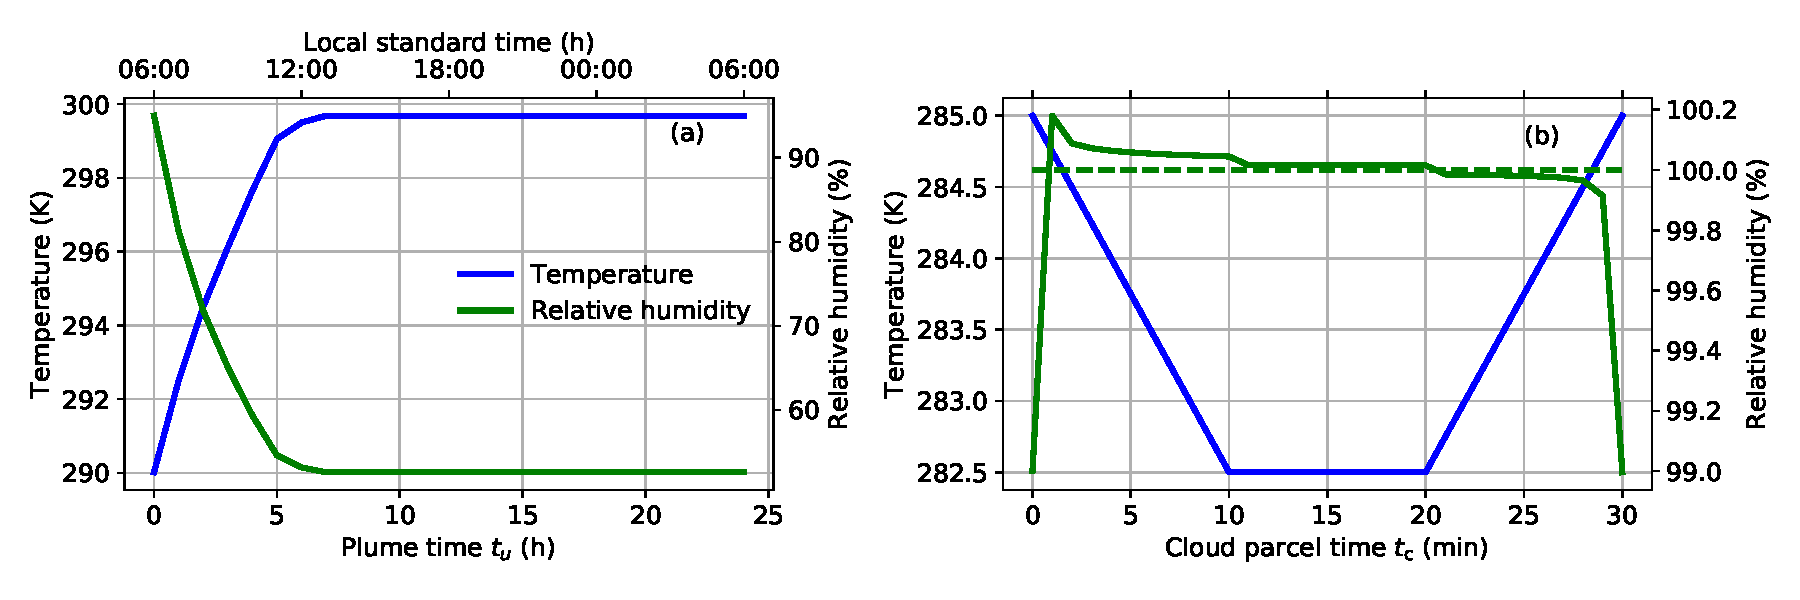
\includegraphics[width=\textwidth]{chap3_figs/fig1.pdf}
	\caption{Temperature and relativity humidity time series in (a)
		urban plume environment and (b) cloud parcel environment. The
		green dashed line in (b) is RH = 100$\%$.}
	\label{fig:env}
\end{figure}

Aerosol emission sources and their compositions are also listed in
Table~\ref{tab:emi}. Note that the composition of aerosol
  emissions from gasoline vehicles was based on
  \citet{somers2004mobile} and \citet{nam2008analysis}. Current
  gasoline vehicles produce tailpipe emissions with higher BC content
  \citep{liggio2012emissions}. However, since both BC and POA have very
  low hygroscopicities ($\kappa=0$ for BC and 0.001 for POA), we do
  not expect that the exact BC/POA split impacted our results for this
  chapter (however this will be important for optical properties).

The mixing state of the aerosol in this simulation evolved because
primary aerosol emissions aged owing to formation of secondary aerosol
and to coagulation processes, while fresh emissions continued to enter
during the first 12 hours of simulation. Overall, this scenario
mimicked the evolution of an air parcel in a polluted urban area, and
we summarized the results, including the mixing state evolution, in
Chapter~\ref{sec:urban_plume}. The full state, including gas-phase
mixing ratios and composition of all computational particles, was
saved hourly to be used as input for the cloud parcel simulations in
step 2.

In addition to the high-emission urban plume case described
  above, we performed a second simulation with reduced initial aerosol
  number concentration and aerosol emissions (5\% of the high-emission
  case) and gas emissions (15\% of the high-emission case) to
  represent a less polluted urban environment. We refer to this case
  as the ``low-emission case''.  Scale parameters relative to the
  high-emission case are summarized in Table~\ref{tab:low-emi}.


\begin{table}[H]
	\centering
		\caption{Scale parameters of gas emission rates, initial and background particle number concentration and aerosol number fluxes emission rates used for low-emission cases (relative to high-emission case)}
	\begin{tabular}{lcccccl}
		\toprule 
		 &  & \multicolumn{2}{c} {Initial/background number conc.} & \multicolumn{3}{c}{Aerosol emission rates} \\
		 \cmidrule(r){3-4}\cmidrule(r){5-7}
		 & Gas emission rates  & Aitken  & Accumulation & Cooking & Diesel & Gasoline  \\
		\midrule
		Scale parameters & 15\% & 5\% & 5\%  & 5\% & 5\% & 5\% \\
		\bottomrule
	\end{tabular}
        \label{tab:low-emi}
\end{table}

For step~2, the hourly output of the simulated aerosol and gas-phase
mixing ratios was used as input for the cloud parcel simulations,
using a prescribed cooling rate. The temperature decreased for
  the first 10 minutes at a rate of $0.25$~$\rm K \, min^{-1}$, which
  corresponds to an updraft velocity of approximately 1~$\rm m \,
  s^{-1}$. The value is calculated by using equation (17.56) in
  \citet{Seinfeld2006a} without consideration of entrainment. The
cooling rate was kept constant for the next 10 minutes, and increased
at the rate of 0.25~$\rm K \, min^{-1}$ for the last 10 minutes. Hence
one cloud cycle consisted of a total of 30 minutes, and we referred to
the elapsed time within the cloud cycle as ``cloud parcel time'',
$t_{\rm c}$. The initial RH for the cloud parcel was 99~$\%$, and it
reached supersaturation within less than 1~min. The parcel became
subsaturated when the cloud began to evaporate at 20 min, and returned
to RH=99$\%$ at the end of the simulation.

Since it is common for air parcels to undergo several cloud cycles
\citep{Barth2003}, we conducted a total of four cloud cycles for
  the high-emission case, which resulted in a total of $25 \times 4 =
100$ cloud parcel simulations. We initialized the aerosol for the
second, third and fourth cloud cycles using the particle population
from the end of the previous cloud cycle. For the gas-phase
  mixing ratios we always used the values from the beginning of the
  first cloud cycle. That is, in choosing this setup, we explored how
  an already processed aerosol population changes further when it is
  exposed to a given gas environment and cooling rate (especially
  focusing on changes in the mixing state) with the only difference
  between cloud cycles being the input aerosol population. We realize
  that this is an idealized setup since in reality the gas phase
  concentrations are likely not the same for subsequent cloud
  cycles. For the low-emission case, we only present the results for
  one cloud cycle.

Lastly, to explore the effects of coagulation, we performed another
set of cloud parcel simulations that included Brownian coagulation,
using the high-emission case as input. For most of our
analysis, we focus on the difference between the particles at the
start of the cloud parcel simulations and the end of the cloud parcel
simulation, after cloud evaporation.

\subsection{Mixing state metrics}
\label{sec:mixing_state_metrics}
The objective of this chapter is to quantify the change of particle
mixing state as a result of cloud processing. The metrics used to
quantify mixing state were developed by \citet{Riemer2013a}. The
mixing state metric $\chi$ is calculated by:
\begin{equation} \label{eq:chi}
    \chi = \frac{{D}_{\alpha}-1}{{D}_{\gamma}-1},
\end{equation}
where $D_{\alpha}$ is the average particle diversity and
$D_{\gamma}$ is the bulk particle diversity.

The calculation of these diversity metrics is based on the
per-particle mixing entropy $H_i$. For an aerosol population of $N$
particles containing $A$ species, the mixing entropy $H_i$ and
particle diversity $D_i$ of particle $i$ are calculated as
\begin{equation}\label{eq:H-i}
    H_i = \sum_{a=1}^{A}-p_i^a {\rm ln}p_i^a  \;\;\;D_i = e^{H_i}, 
\end{equation}
where $p_i^a$ is the mass fraction of species $a$ in particle
$i$. Expanding $D_i$ to the whole population, $D_\alpha$ and
$D_{\gamma}$ are defined as
%  \label{alpha}
  \begin{align}
    H_\alpha &= \sum_{i=1}^N p_i H_i\;\;\;&D_\alpha= e^{H_\alpha}, \label{eq:H-alpha}\\
    H_\gamma &= \sum_{a=1}^A -p_a H_i\;\;\;&D_\gamma= e^{H_\gamma}, \label{eq:H-gamma}
  \end{align}
where $p_i$ and $p_a$ are the mass fractions of particle $i$ and
species $a$ in the population. For externally mixed populations where
particles contain only one species, $D_\alpha =1$ and $\chi =0\%$. For
internally mixed population where each particle has the same
composition as the bulk, $D_\alpha = D_\gamma $ and $\chi =100\%$. In
the ambient atmosphere, aerosols are neither completely internally nor
externally mixed and intermediate mixing states are common
\citep{Healy2014,Ye2018,Ching2019}. For regions close to emission
sources, $\chi$ is expected to be lower, while $\chi$ is larger in air
masses dominated by an aged aerosol. 

The mixing state metrics $\chi$ defined in this chapter used the
abundance of model chemical species as the basis for calculating
particle mass fractions in
Equations~(\ref{eq:H-i})--(\ref{eq:H-gamma}), i.e. sulfate, nitrate,
ammonium, POA, etc., excluding aerosol water. Other choices for
defining ``species'' are possible, for example \citet{Ching2017} used
two surrogate species, hygroscopic and non-hygroscopic species, as the
basis for $\chi$. Furthermore, \citet{Zheng2021} compared $\chi$ based
on the mixing of model chemical species, of hygroscopic and
non-hygroscopic species, and of absorbing and non-absorbing species.

\section{Simulation results}
\label{sec:results}
\subsection{Urban plume simulation with PartMC-MOSAIC}
\label{sec:urban_plume}

This section summarizes the results from the urban plume simulations
to provide context for the cloud parcel simulations discussed in the
remainder of the chapter. Figure~\ref{fig:urban_plume} shows selected
quantities from the high-emission urban plume simulation. The
total particle number concentration $N_{\rm a}$ increased initially
due to the emission of primary particles, reached a maximum of 15,295
$\rm cm^{-3}$ at $t_{\rm p} = 12$~h, then decreased because the
emissions ceased, and both dilution and coagulation reduced the
particle number concentration. Similarly, BC and POA mass
concentrations increased for the first 12~h due to emission, and
decreased thereafter due to dilution with the background, just as
Figure~\ref{fig:urban_plume}b shows. The time series of the secondary
aerosol species sulfate and SOA were determined by the interplay of
loss by dilution and photochemical production. The ammonium nitrate
mass concentration was determined by the gas concentrations of its
precursors, $\rm HNO_3$ and $\rm NH_3$, temperature and RH. Mixing
ratios of $\rm SO_2$, $\rm O_3$ and $\rm H_2O_2$ are shown in
Figure~\ref{fig:urban_plume}c for reference because they are directly
involved in the in-cloud sulfate formation as discussed in
Chapter~\ref{sec:cloud}.

Figure~\ref{fig:urban_plume}b only displays the bulk composition of
the aerosol, while the mixing state information available from the
particle-resolved output remains hidden. Figure~\ref{fig:urban_plume}d
provides insight into the evolution of aerosol mixing state as
quantified by the mixing state metrics introduced in
Chapter~\ref{sec:mixing_state_metrics}. At $t_{\rm u} = 0$, the
particle population was completely internally mixed, and therefore the
mixing state index $\chi$ was initially 100\%.

From Equation~\ref{eq:chi}, we recall that $\chi$ is determined by the
ratio of $D_{\alpha}$ and $D_{\gamma}$. Figure~\ref{fig:urban_plume}d
indicates that both $D_{\alpha}$ and $D_{\gamma}$ started out low,
which is consistent with the aerosol initially only containing a small
number of species, both on a per-particle level and on a population
level, see Table~\ref{tab:emi}. Over the course of the simulation,
both $D_{\alpha}$ and $D_{\gamma}$ increased, but at different rates,
which led to changes in $\chi$ that we can interpret as changes in
mixing state. The initial decrease in $\chi$ to about 50\% was caused
by the emission of fresh combustion particles, containing BC and
POA. These emissions continued for the first 12~h of simulation, but
at the same time coagulation and secondary aerosol formation occurred,
which (at least initially) efficiently increased the average
per-particle diversity $D_{\alpha}$. Overall, this
led to a more internally mixed population, with $\chi$ increasing to
72\% at 10~h. After this, dilution became relatively more important,
introducing background particles, and ammonium nitrate evaporated
almost entirely towards the end of the simulation. These combined
processes resulted in a slow decrease in $\chi$ to 64\% at the end of
simulation.

\begin{figure}
    \centering
    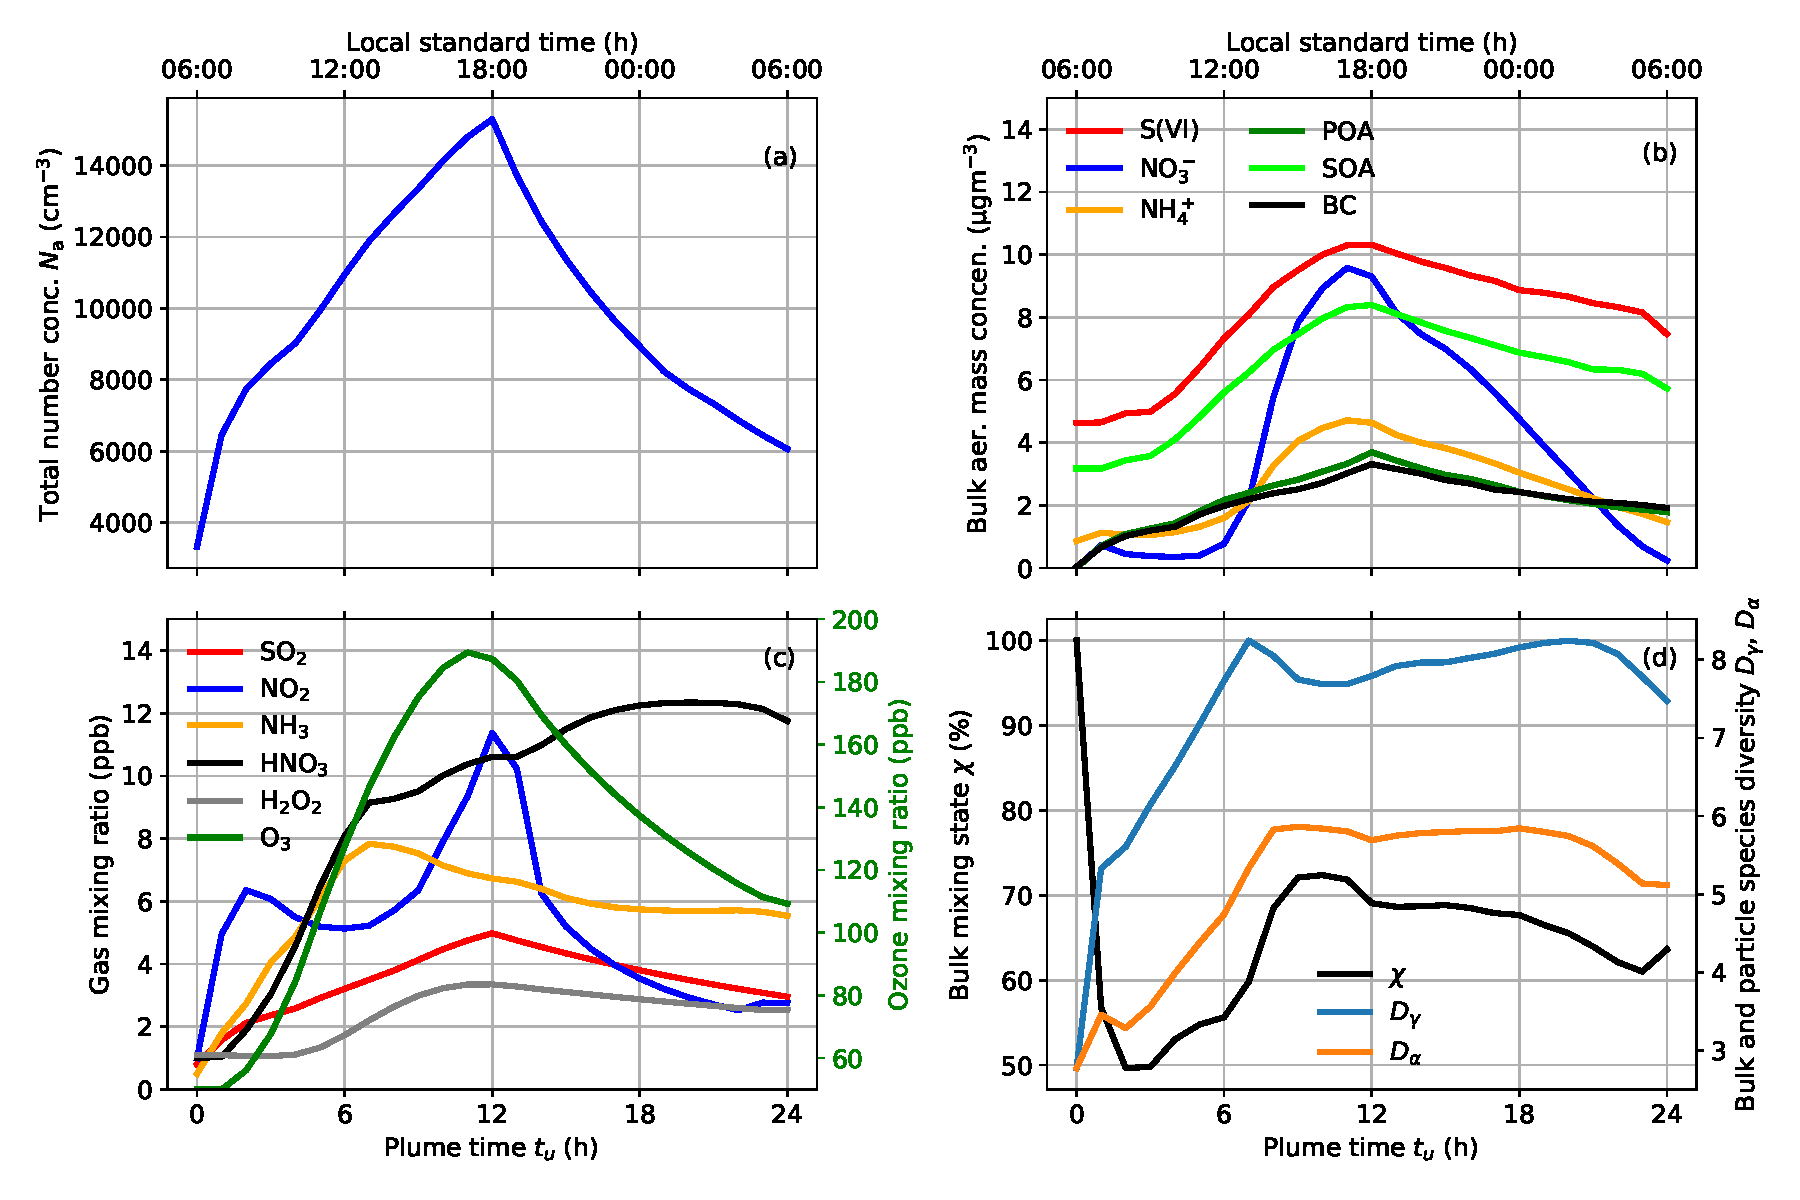
\includegraphics[scale=0.50]{chap3_figs/fig2.pdf}
    \caption{Temporal variation of (a) total number concentration, (b)
      mass concentrations of selected aerosol species, (c) mixing
      ratios of selected gas-phase species and (d) aerosol mixing
      state metrics for the high-emission case. }
    \label{fig:urban_plume}
\end{figure}

The corresponding figure for the low-emission case is shown as
Figure~\ref{fig:sup1}. As expected, for
this case, the aerosol number and mass concentrations and the
gas-phase concentrations were reduced compared to the high-emission
case. For example, the maximum aerosol number concentration at
$t=12$~h only reached to about 1000~$\rm cm^{-3}$ and the maximum $\rm
SO_2$ mixing ratio was only 1.2~ppb. The mixing state metrics
(Figure~\ref{fig:sup1}d) ranged between 40\% and 78\%.
  
  \begin{figure}
    \centering
    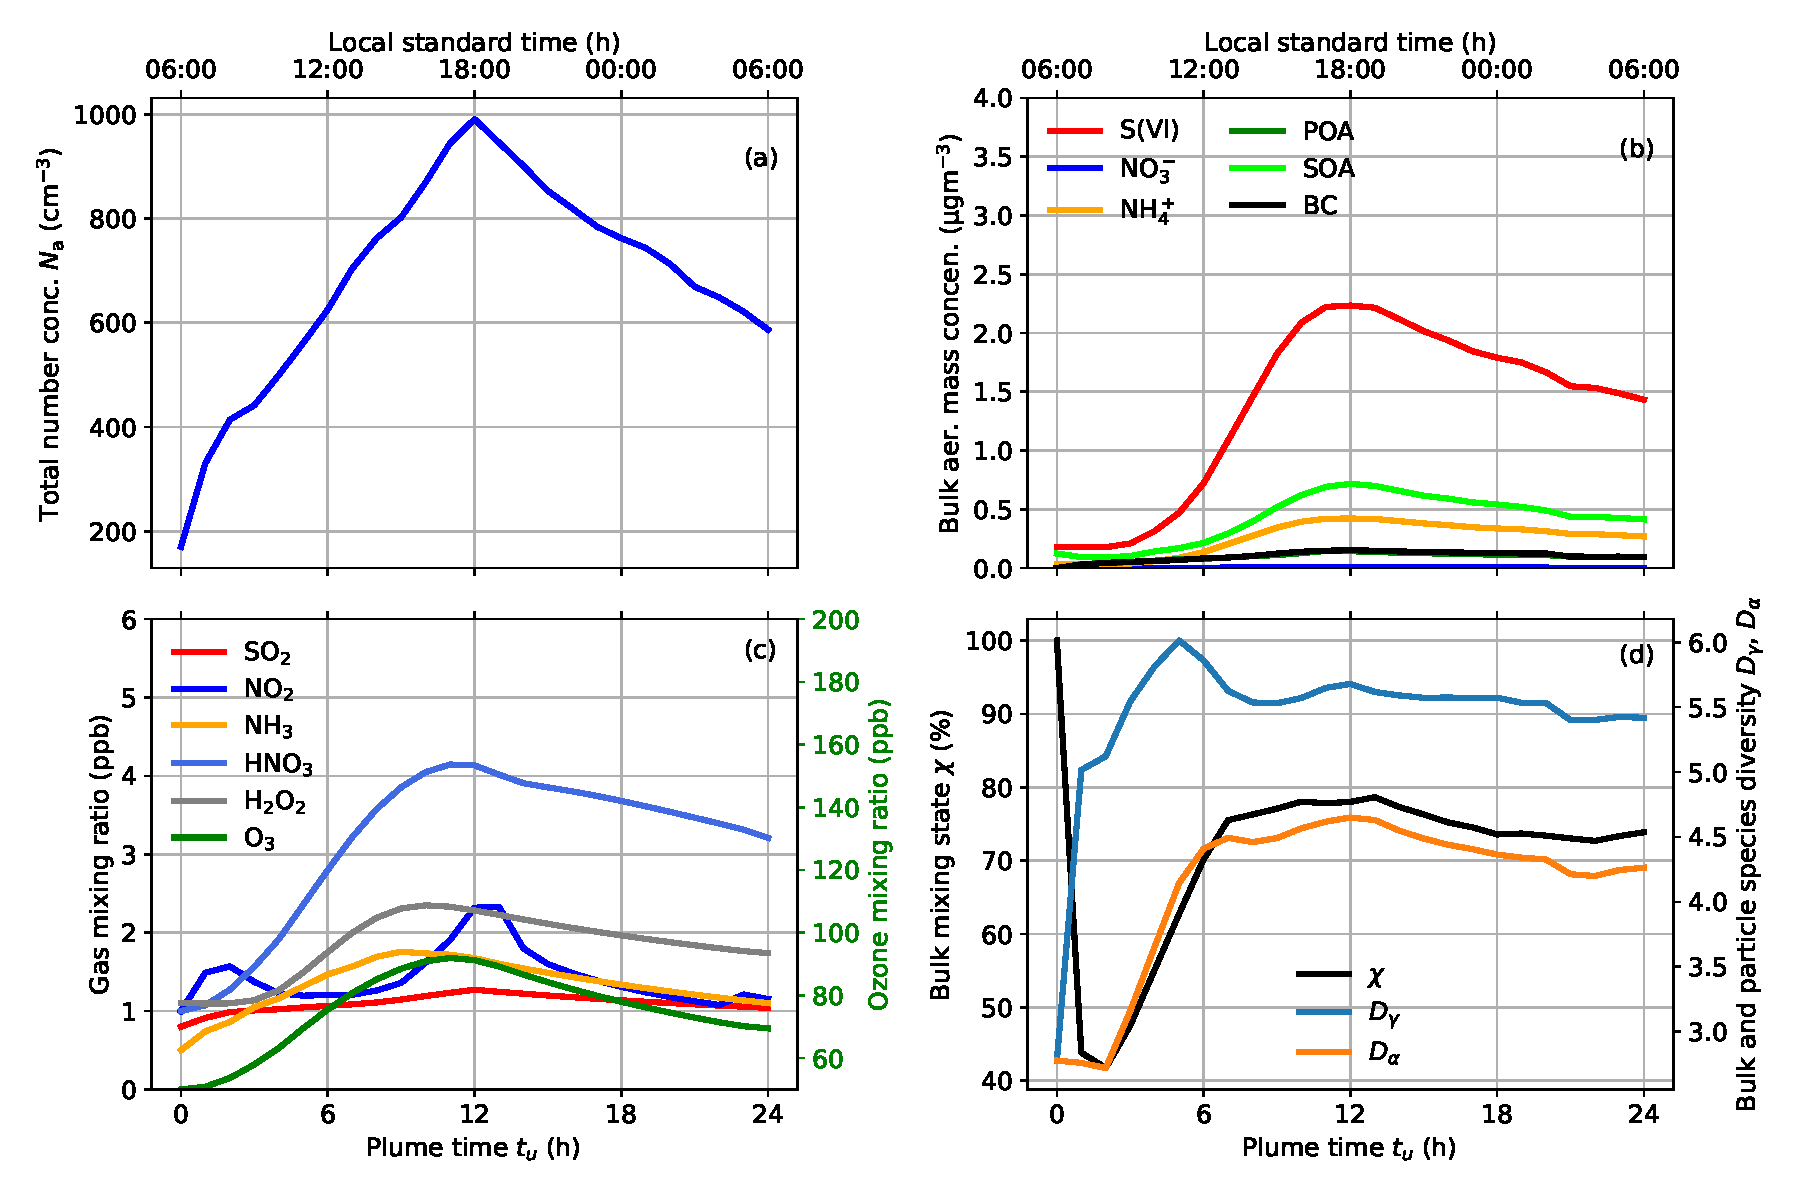
\includegraphics[scale=0.5]{chap3_figs/fig_sup1.pdf}
    \caption{Temporal variation of (a) total number concentration, (b)
      mass concentrations of selected aerosol species, (c) mixing
      ratios of selected gas-phase species and (d) aerosol mixing
      state metrics for the low-emission case.}
    \label{fig:sup1}
\end{figure}

\subsection{Aerosol composition changes during cloud processing}
\label{sec:cloud}
As described in Chapter~\ref{sec:urban_plume}, for each hourly output
from the urban plume simulations, cloud cycles were simulated using
the same temperature profile, shown in Figure~\ref{fig:env}b.
Each cloud parcel simulation was exposed to the same cooling
  rate but differed in their initial conditions of aerosol populations
  and gas-phase concentrations. Figure~\ref{fig:cases-gases} compiles
  the initial conditions of selected gas-phase species for the cloud
  parcel simulations using the high-emission case. Each color marks a
  specific cloud parcel case, which corresponds to a specific plume
  time $t_{\rm u}$. The ranges were consistent with conditions found
  in polluted urban regions, such as Haikou in southern China, with
  annual average mixing ratios of 2 ppb $\rm SO_2$ and 7 ppb $\rm
  NO_2$ \citep{wang2014spatial}, and Kanpur in Northern India, with
  annual average mixing ratios of 3 ppb $\rm SO_2$ and 5.7 ppb $\rm
  NO_2$ \citep{gaur2014four}. In this section, we first illustrate
the compositional changes during cloud processing, using the aerosol
population from the high-emission case at $t_{\rm u} =12$~h
as the initial conditions for the cloud parcel simulation, and focus
on the first cloud cycle ($N_{\rm cycle}=1$).

 \begin{figure}
    \centering
    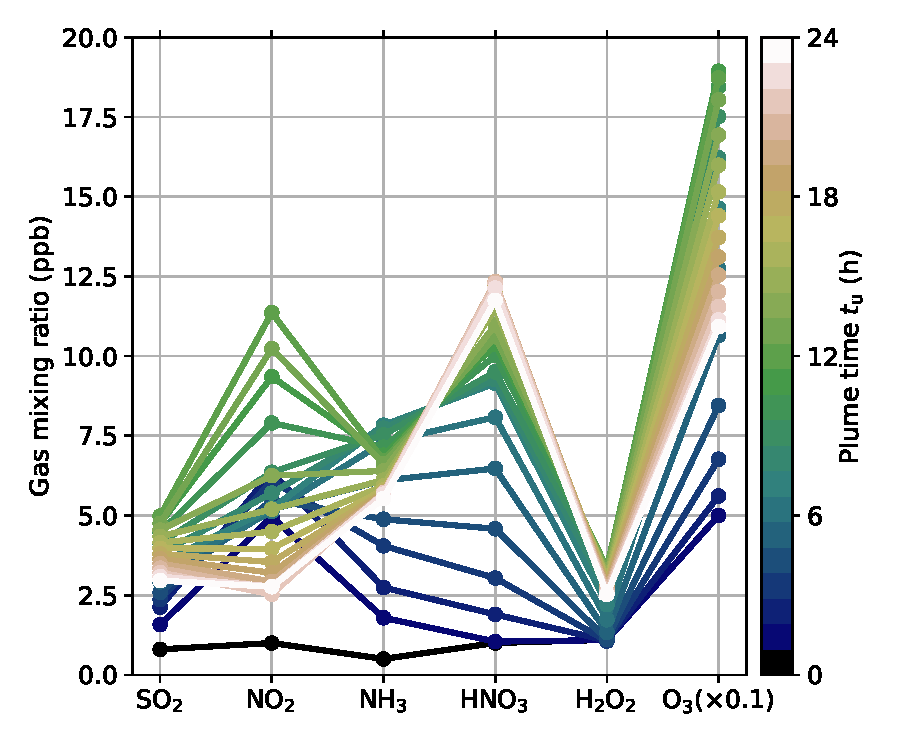
\includegraphics[scale=0.6]{chap3_figs/fig3.pdf}
    \caption{Initial conditions for selected gas-phase species
        for the cloud parcel simulations (high-emission case). Colors
        indicate the different plume hours. Note that the mixing ratio
        for $\rm O_3$ is multiplied by 0.1 to be able to use the same
        scale on the ordinate as for the other gases.}
    \label{fig:cases-gases}
\end{figure}

Figure ~\ref{fig:cloud_env}a shows the evolution of several key
variables for this case. The initial RH for each cloud parcel
  simulation was 99\%, and the aerosol water content of each particle
  was adjusted for RH=99\% based on the dry aerosol composition. The
  parcel reached supersaturation within 1~min. During the
first 10~min the liquid water content increased and reached a maximum
of 1.23 $\rm g \, kg^{-1}$ at 10 min. We determined the cloud droplet
number concentration following the strategy used in \citet{ching2012impacts},
where particles with wet diameter larger than 2 $\rm \mu m$ were
classified as cloud droplets. As shown in the figure, the cloud
droplet number concentration (CDNC) was 2011 $\rm cm^{-3}$ at the time
when the maximum supersaturation was reached. This number
concentration decreased somewhat as the relative humidity slowly
relaxed to saturation, which can be explained by the so-called
``inertial effect'' \citep{Chuang1997, Nenes2001}. This refers to
droplets with diameter larger than 2 $\rm \mu m$ that were not truly
activated, i.e., they had a critical diameter larger than 2 $\rm \mu
m$ and this critical diameter was not reached during the simulation
time.  After 20~min, as the RH dropped below 100\%, the cloud droplet
number concentration declined faster and the cloud evaporated.

The CDNC is comparatively high for the example shown in
Figure~\ref{fig:cloud_env}, since we started out with a large aerosol
number concentration of over 15,000~$\rm cm^{-3}$. CDNC of this
magnitude were observed, for example, during the IMPACT field campaign
\citep{brenguier2011cloud}.  Using aerosols from other plume hours as
inputs yielded CDNC below 2000 $\rm cm^{-3}$, as shown in
Figure~\ref{fig:max_ss-cycle} (but always larger than 1000~$\rm
cm^{-3}$). For the low-emission case, the CDNC were much lower,
between 100 and 640 $\rm cm^{-3}$, consistent with observations in
more moderately polluted urban environments \citep{ahmad2013long}.

\begin{figure}
    \centering
    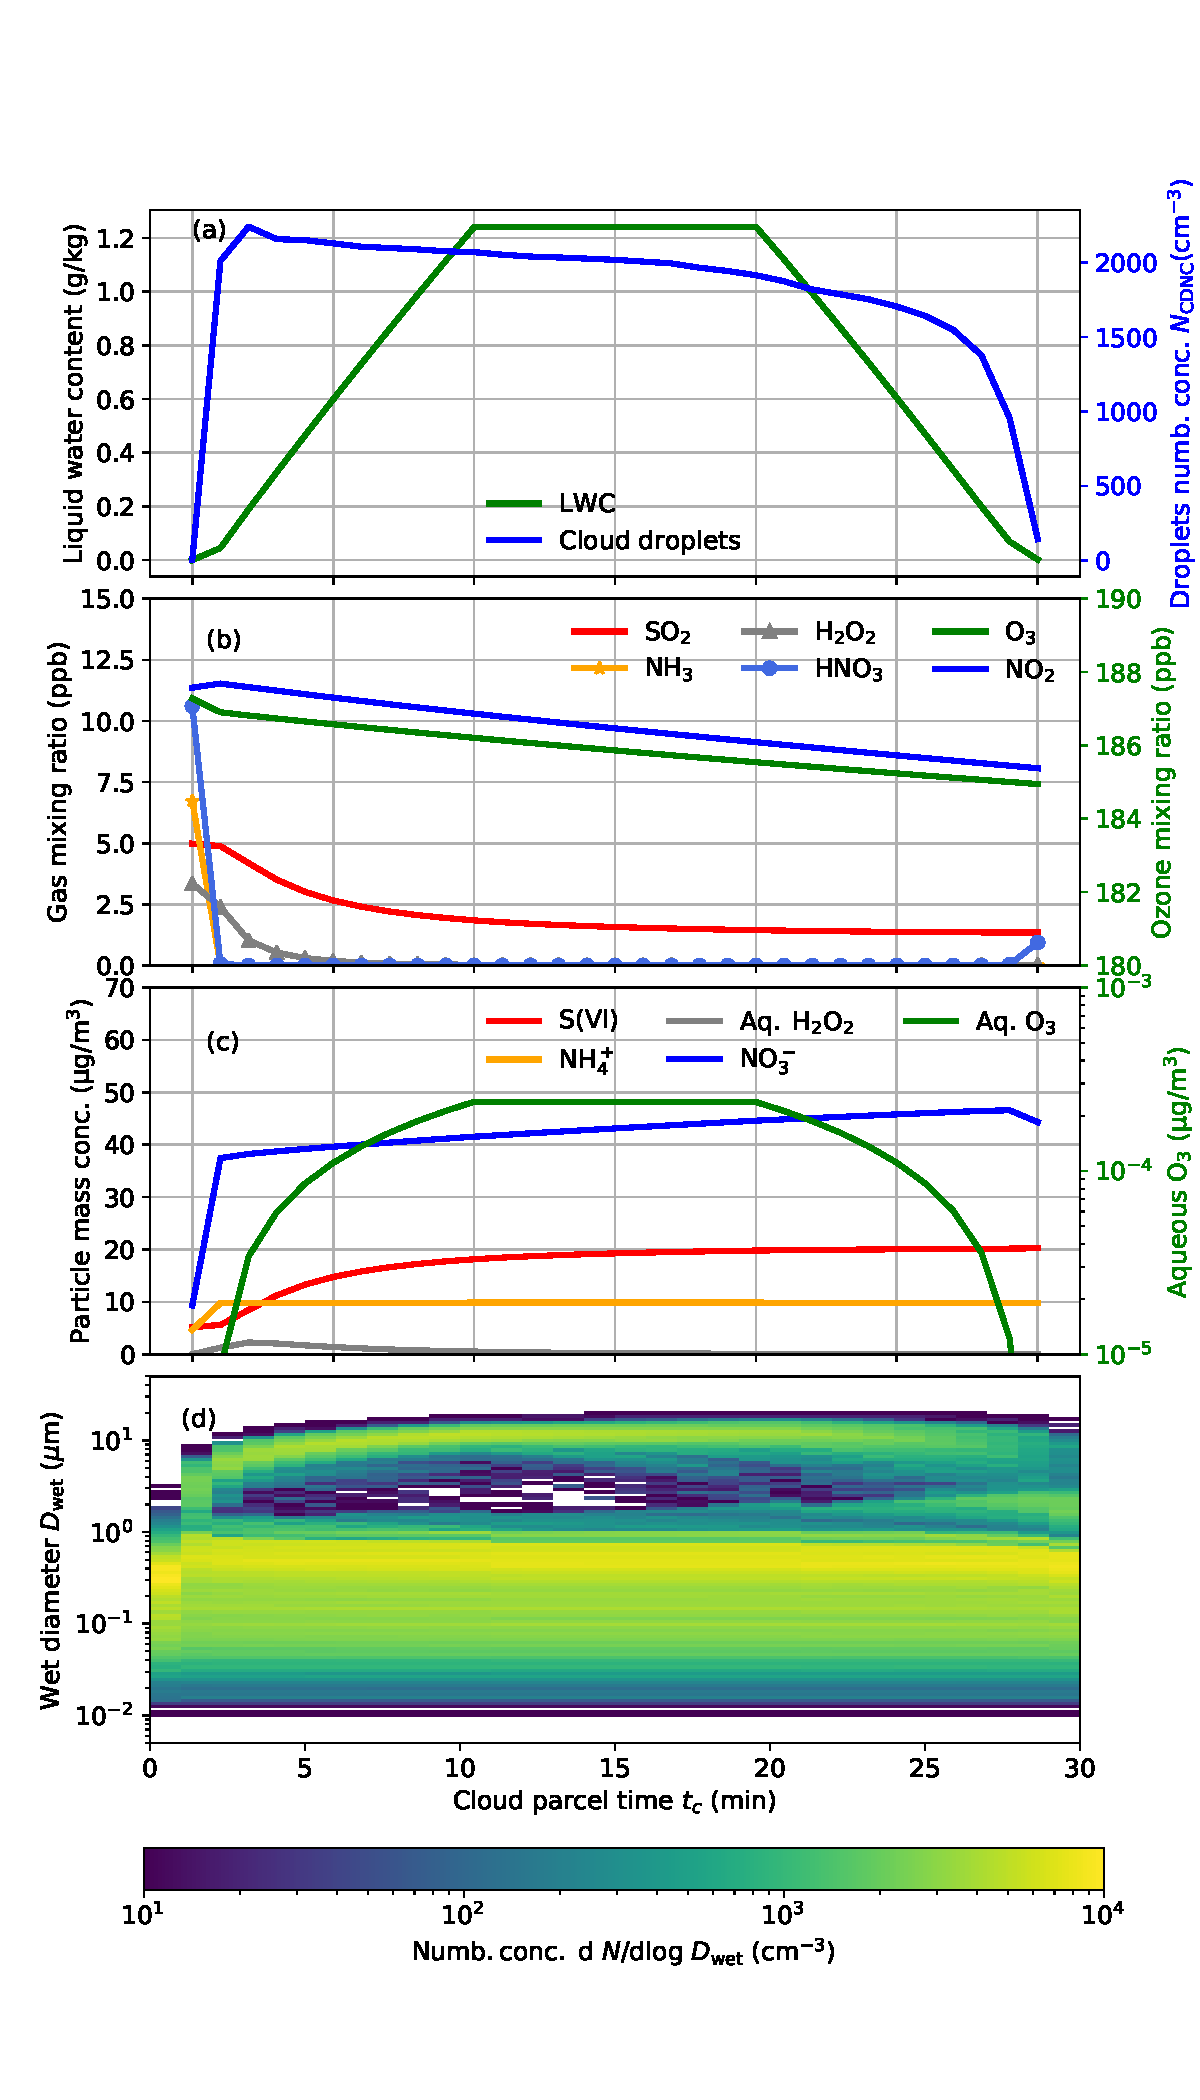
\includegraphics[scale=0.50]{chap3_figs/fig4.pdf}
    \caption{The evolution of (a) liquid water content (LWC) and cloud
      droplet number concentration (b) mixing ratios of key gas-phase
      species (c) key aqueous-phase species and (d) number
      concentration with respect to wet diameter. Results are for the
      aerosol population at $t_{\rm u} =12$~h (high-emission
        case) and for $N_{\rm cycle}=1$.}
    \label{fig:cloud_env}
\end{figure}

\begin{figure}
    \centering
    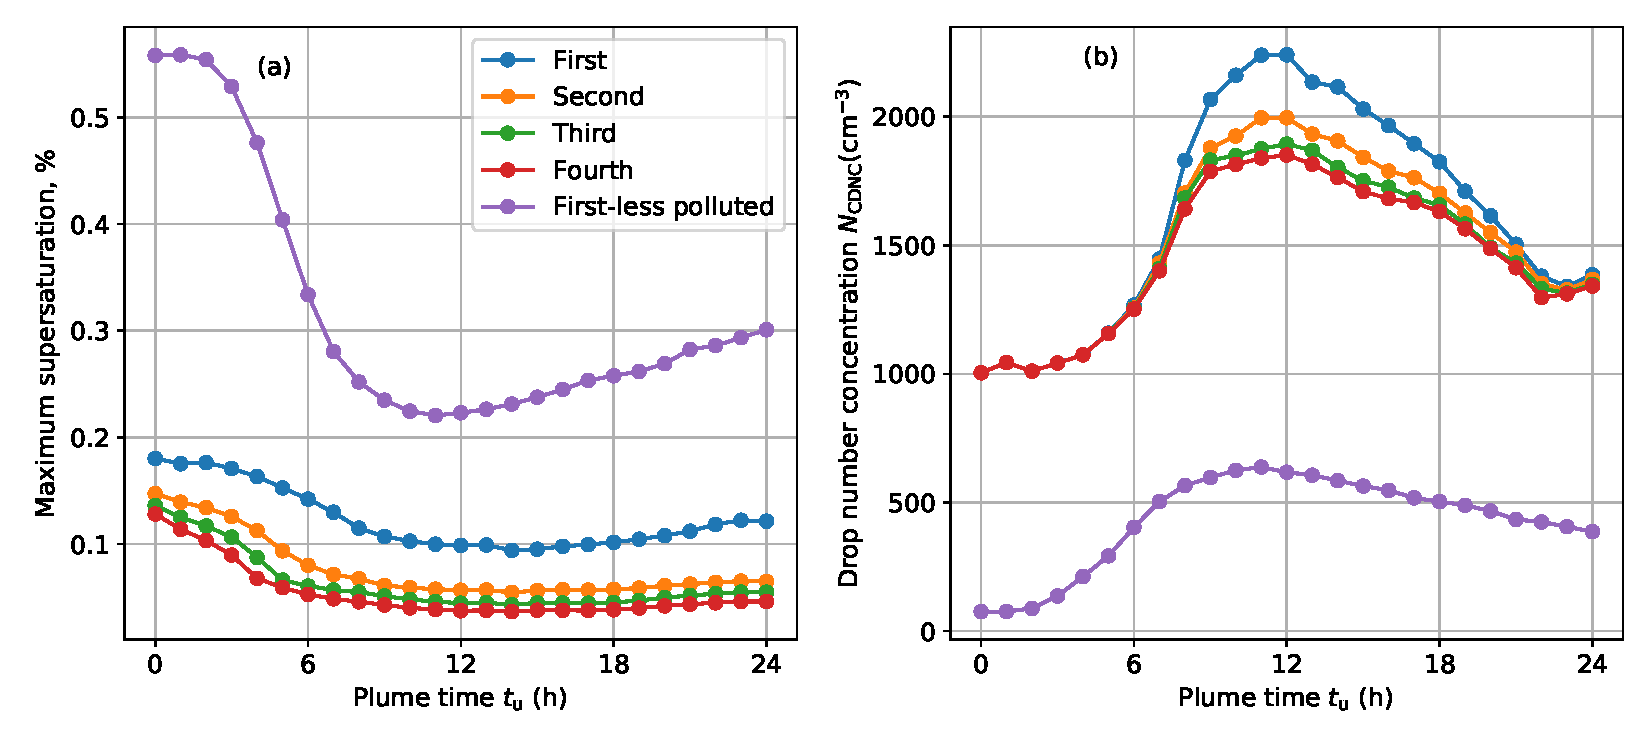
\includegraphics[scale=0.5]{chap3_figs/fig_sup5.pdf}
    \caption{(a) Maximum supersaturation reached in the cloud parcel
      and (b) cloud droplet number concentration in the four cycles.}
    \label{fig:max_ss-cycle}
\end{figure}

Figure~\ref{fig:cloud_env}b and Figure~\ref{fig:cloud_env}c show the
evolution of several key gas and aqueous-phase species. Ammonia in the
gas-phase dissolved and immediately formed ammonium. Aqueous-phase
$\rm NH_4^+$ increased from 4.7 to 9.8~$\rm \mu g\;m^{-3}$. Nitrate
increased rapidly from 9.3 to 37.4~$\rm \mu g\;m^{-3}$ at the
beginning due to the uptake of $\rm HNO_3$. These processes are
explained by the R1-R10 reactions in Table~S1. After
this, nitrate was further formed through reaction R15.

The dissolved sulfur dioxide formed $\rm SO_3^{2-}$ and $\rm HSO_3^-$,
and could be oxidized to sulfate by aqueous-phase $\rm H_2O_2$ or $\rm
O_3$ through R11-R15. The sulfate aqueous formation rates are highly
pH-dependent, and the $\rm H_2O_2$ oxidation reaction R13 is dominant
for pH lower than 5, while the $\rm O_3$ pathway R12 becomes more
important for pH higher than 6 \citep{Seinfeld2016, Shao2019}. For the
cases shown here, the cloud droplets were acidic, and therefore the
oxidation by $\rm H_2O_2$ dominated. Sulfur dioxide in the gas-phase
decreased from 4.98 to 1.94~ppb, and the S(VI), including $\rm
SO_4^{2-}$ and $\rm HSO_4^-$, increased from 5.16 to 20.23~$\rm \mu
g\;m^{-3}$ during the simulation period.

The evolution of the number size distributions based on wet diameter
is illustrated in Figure~\ref{fig:cloud_env}d. At $t_{\rm c} =
0$, the size distribution peaked at 0.3~$\rm \mu m$.  As discussed
above, in less than 1~min, a subset of the particles activated to form
cloud droplets and the particle size distribution evolved from
initially unimodal to bimodal, with the first peak representing the
interstitial (not activated) particles and the second peak
representing the cloud droplets. The interstitial aerosol remained
unchanged since this simulation did not include coagulation. We will
investigate the impact of coagulation further in
Chapter~\ref{sec:coag}. With increasing liquid water content and
aqueous chemistry processes occurring, the cloud droplets continued to
grow and the droplet mode peaked at 11 $\rm \mu m$ at 20~min.

Next, we will turn to the changes in aerosol size distributions. To
provide a summary of the 25 individual cloud parcel simulations, we
show here the average over all 25 scenarios with the variability
amongst cases indicated by the standard deviation (colored band).
Figure~\ref{fig:size_number} shows the number and mass concentration
as a function of dry diameter before entering the cloud and after each
cloud cycle for the high-emission case. After the first cloud
cycle, a second mode appeared for the dry number distribution,
transforming the unimodal number distribution that peaked at a dry
diameter of 0.1~$\rm \mu m$ to a bimodal distribution with a second
peak at 0.3~$\rm \mu m$.  For each additional cloud cycle, the peak of
the second mode kept moving to larger diameters and reached 0.5~$\rm
\mu m$ after the fourth cloud cycle.

The number size distribution of the cloud droplet residuals
  peaked at a dry diameter of 0.3~$\rm \mu m$ after the first cloud
  cycle, which is consistent with field observations
  \citep{fast2019impact, ditas2012aerosols, ge2012effect}. For
  subsequent cloud cycles, the diameters increased further, because
  each cycle added more secondary aerosol mass on the already
  cloud-processed particles. This may not be representative for real
  clouds, where particle growth may be limited by gas precursors or
  oxidants and where entrainment occurs. However, cloud droplet
  residuals as large as 1~$\rm \mu m$ aerodynamic diameter were
  observed for particles collected at a mountain site in Southern
  China \citep{lin2017situ}.

In order to quantify the diameter changes, we define the mean diameter
$\bar{D}$ as
\begin{equation}
	\bar{D}=\frac{\sum_{i=1}^{n} N_i D_i}{N_{\rm total}},
\end{equation}
where $i$ is the particle index, $n$ is the total number of computational
particles, $N_{\rm total}$ is the total number concentration, $N_i$
and $D_i$ are the number concentration and diameter of computation
particle $i$. The increase in diameter was largest for the first
cycle, where $\bar{D}$ increased 24$\%$ and grew from 0.1 to
0.124~$\rm \mu m$. The fourth cycle only led to a 5\% mean diameter
increase. For the mass, as shown in Figure~\ref{fig:size_number}b,
distributions are dominated by the larger particles, as
expected. Similar to the trend seen in the number size distribution,
the mass increased most in the first cycle. The dry mass
  concentration, averaged over all 25 cases, increased from 21.2 to
  67.2~$\rm \mu g$ $\rm cm^{-3}$ in the first cycle, which corresponds
  to 217$\%$. After the fourth cycle, the mass increased from 110.4 to
  152.8~$\rm \mu g$ $\rm cm^{-3}$ (38\%).

\begin{figure}
    \centering
    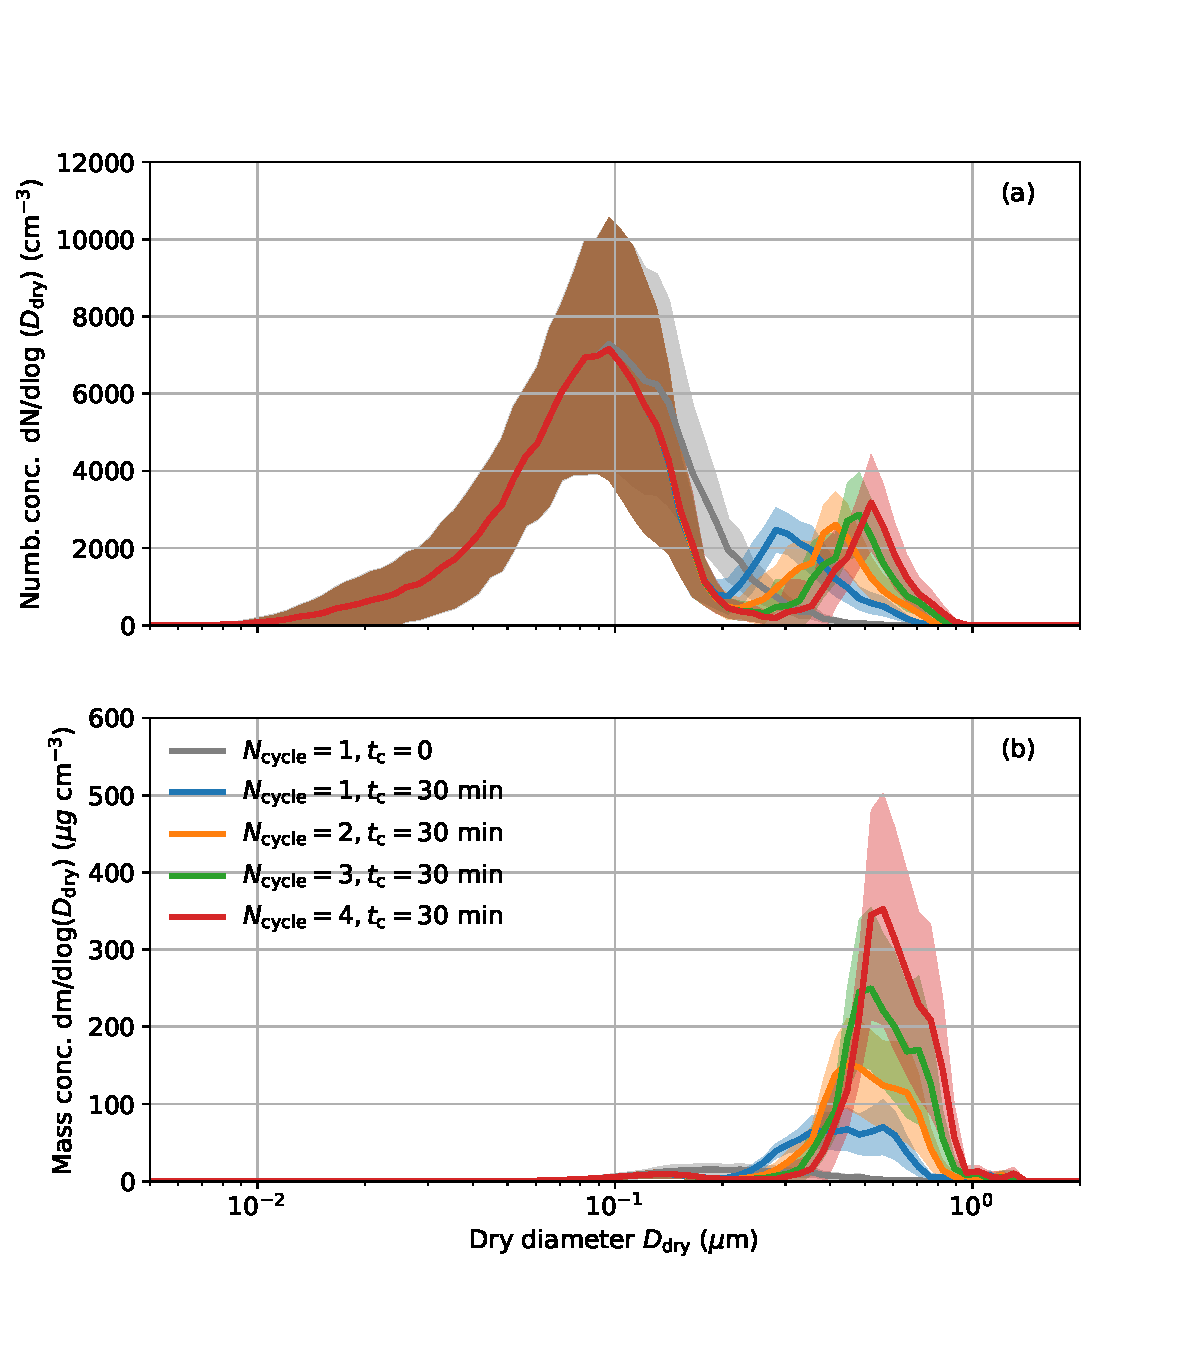
\includegraphics[scale=0.45]{chap3_figs/fig5.pdf}
    \caption{(a) Number and (b) mass size distribution with respect to
      dry diameter before the first cloud cycle and after each
      subsequent cloud cycle (high-emission case). The solid
      lines are the averaged distributions of all 25 cases for each
      cloud cycle. The shaded area represents the 1$\sigma$ region of
      the average. The grey line is the distribution at $t_{\rm c}= 0$
      min, and the other lines are the distributions at the end of
      each cloud cycle. The composition of the particles was evaluated
      at RH = 99\%. The brown shading in (a) is due to the
        overlapping colors of different cycles.}
    \label{fig:size_number}
\end{figure}

The size distributions for the low-emission case are shown in
Figure~\ref{fig:sup2}. The average mode diameter of the cloud droplet
mode after the first cycle is somewhat larger ($\sim0.35$~$\rm \mu m$)
than in the high-emission case even though the gas-phase precursor
concentrations were lower. This can be explained by the fact that the
CDNC was substantially lower than in the high-emission case, and the
gas-phase concentrations were still high enough to allow more
secondary aerosol mass to form per droplet.
  
  \begin{figure}
    \centering
    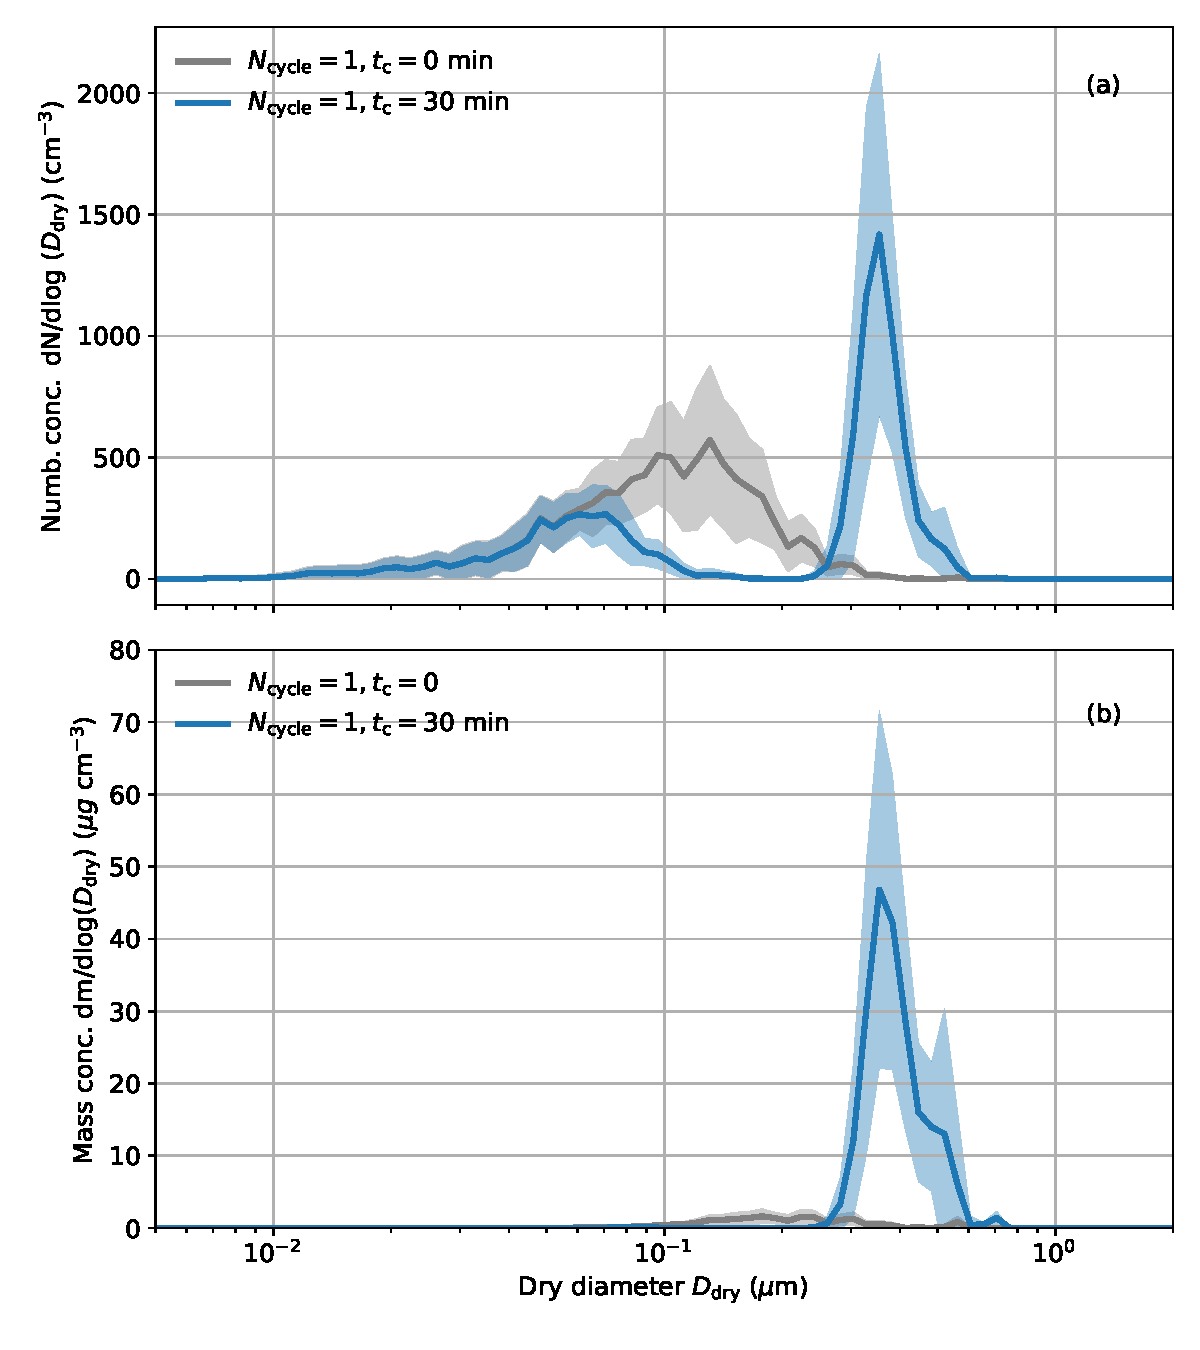
\includegraphics[scale=0.5]{chap3_figs/fig_sup2.pdf}
    \caption{(a) Number and (b) mass size distribution with respect to
      dry diameter before (grey) and after (blue) the first cloud
      cycle for the low-emission case.  The solid lines are the
      averaged distributions of all 25 cases for each cloud cycle. The
      shaded area represents the 1$\sigma$ region of the average.  are
      the distributions at the end of each cycle. The composition of
      the particles was evaluated at RH = 99\%.}
    \label{fig:sup2}
\end{figure}

Figure~\ref{fig:size_mass} shows the size-resolved mass fractions
averaged over the 25 cases for each cloud simulation at the beginning
of the first cloud cycle (grey) and at the end of the fourth cloud
cycle (RH=99\%) in high-emission cases.  As expected, no change in the
size-resolved composition occurred for particles smaller than about
$0.1$~$\rm \mu m$, as these particles remained interstitial
aerosol. For the activated particles, the sulfate mass fraction
increased from $9.6\%$ to $38.7\%$ in the size range of
0.14--0.25~$\rm \mu m$, and the nitrate mass fraction increased from
$2.8\%$ to $56.8\%$ in the size range of 0.21--0.89~$\rm \mu
m$. \citet{ge2012effect} also found that particles were more
  enriched with nitrate and sulfate after aqueous processing from 
  samples collected from Central Valley of California. For the
particles in size range of 0.1--0.2~$\rm \mu m$, the fraction of
inorganic and SOA species decreased and the fraction of POA and BC
species increased after cloud processing. This can be explained by the
fact that there were two groups of particles in this size range, one
group with mainly inorganic species and SOA, and the other group with
mainly BC and POA. Particles in the first group were activated and
grew larger due to cloud processing. Because more ammonium sulfate and
nitrate was produced than SOA, the fraction of inorganics increased
more than the SOA fraction. As a result, in the size range of
0.7--0.9~$\rm \mu m$, particles transferred from organics-dominant to
inorganics-dominant. The reduced SOA mass fraction in this size
  range can also be explained by the simplified aqueous SOA formation
  mechanism in the current study, which for example does not include
  the formation of IEPOX-derived organosulfates that have shown to be
  important in the ambient atmosphere \citep{hatch2011measurements}.
In summary, even in the same size ranges (here 0.1--0.2~$\rm \mu m$),
particles with different compositions can evolve differently. This is
challenging to resolve for models that represent composition with
one-dimensional distributions, assuming internally mixed particles
within one size bin, and further work is needed to investigate
  the bias that may be introduced by this assumption.

For our current work, the cloud simulations were set up using the
temperature profile shown in figure~\ref{fig:env}b. Specifically, we
considered a cloud that was maintained for about 30~min. In the real
environment, clouds may last from minutes to days, depending on cloud
type and the surrounding environment \citep{Cotton2011}, and they may
also experience a range of different updraft velocities. Since the
largest rate of secondary mass formation occured within a few minutes
after the cloud formed, shortening the cloud parcel time did not
impact the conclusions as long as the first few minutes were
captured. With longer cloud lifetime, secondary aerosol mass formation
may continue, provided that the reactants are not depleted. Variations
in updraft velocities/cooling rates will result in different maximum
supersaturations, and hence differences in the subpopulations of
activated particles. We did not explore these sensitivities here to
keep the scope focused on the changes of particle populations after
typical but complete cloud processes.

\begin{figure}
    \centering
    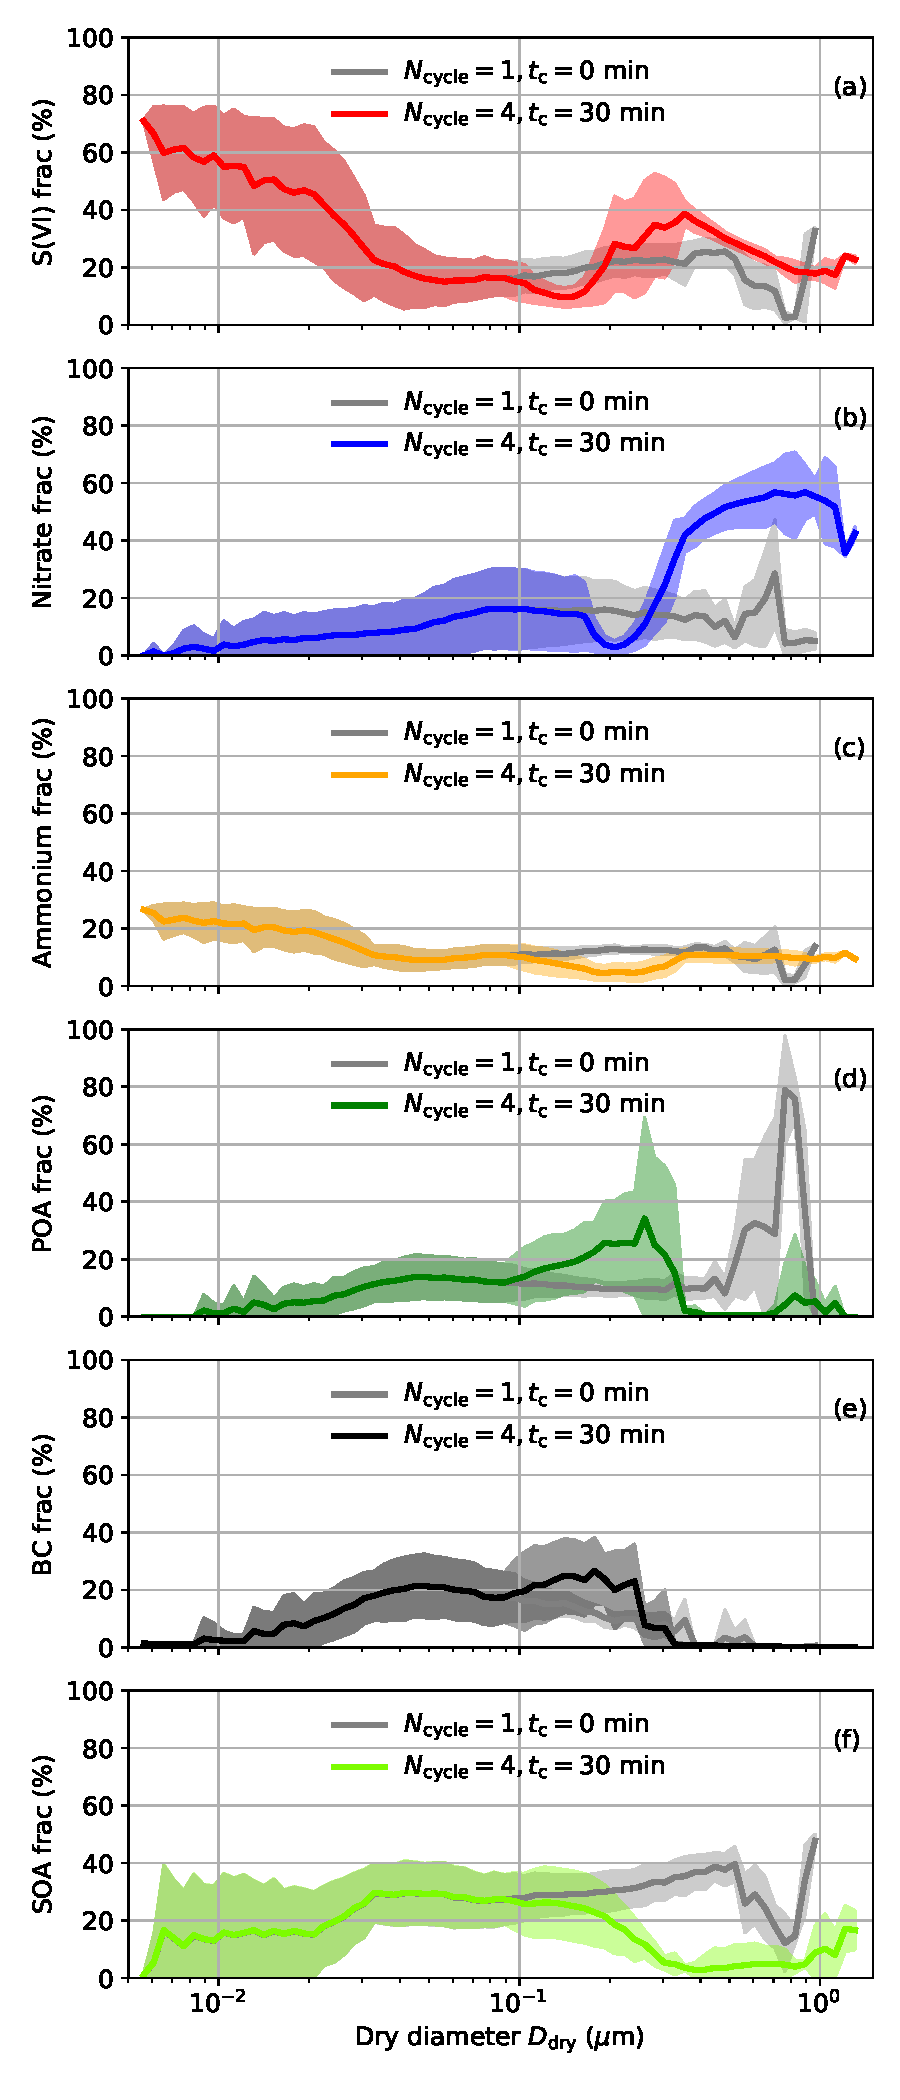
\includegraphics[scale=0.60]{chap3_figs/fig6.pdf}
    \caption{Size-resolved mass fractions of (a) S(VI), (b) nitrate,
      (c) ammonium, (d) POA, (e) BC and (f) SOA at $t_{\rm c}=0$~min
      of the first cloud cycle (grey lines), and $t_{\rm c}=30$~min
      after the fourth cloud cycle (colored lines) for the
        high-emission case.  Solid lines are the average values of
      all 25 cases for each cycle and the shaded band represents the
      range of one standard deviation. The composition was
        evaluated at RH = 99\%.}
    \label{fig:size_mass}
\end{figure}

The previous analyses showed the size-resolved state of the
aerosol. However, even within a certain size range, particles can
exhibit differences in composition, and we introduced this earlier as
the aerosol mixing state. With our particle-resolved modeling approach,
we are able to resolve this detail and quantify how aerosol mixing
state changes with cloud processing. In order to visualize the change
in aerosol mixing state, Figure~\ref{fig:su_2d} displays the
two-dimensional size distribution of sulfate mass fraction $n(D_{\rm
  dry}, w_{\rm SO_4})$ for the example of two plume hours $t_{\rm u} =
0$ and $t_{\rm u} = 12$~h, before entering the cloud simulation and
after four cloud cycles. At the beginning of the urban plume
simulation ($t_{\rm u} = 0$~min), all particles had the same
composition, and $n(D_{\rm dry}, w_{\rm SO_4})$ was 36\% across the
entire population (Figure~\ref{fig:su_2d}a). Over the course of the
urban plume simulation, $n(D_{\rm dry}, w_{\rm SO_4})$ was controlled
by condensation, coagulation and dilution processes, and it became
more diverse as shown in Figure~\ref{fig:su_2d}b. The aerosol primary
emissions consisted of BC- and POA-containing particles (from
gasoline, diesel and cooking emissions), which over time became coated
with sulfate (as well as nitrate and SOA), resulting in particles with
sulfate mass fraction of about 20\% or less.  In
Figure~\ref{fig:su_2d}b, particles in the size range of 0.01--0.2~$\rm
\mu m$ appeared with a sulfate mass fraction of 70\%. These are
background particles that were introduced into the simulation by
dilution with their initial SOA content (model species API1) having
evaporated. The low particle number concentrations in between these
main particle types originate from coagulation events.

Figure~\ref{fig:su_2d}c and Figure~\ref{fig:su_2d}d show the
distributions after four cloud cycles. Note that the initial
concentrations of the gas-phase species between the two plume hours
differed as shown in Figure~\ref{fig:urban_plume}c. Using the
population at $t_{\rm u} = 0$~h, all particles started with the same
composition, and particles with diameters larger than 0.1~$\rm \mu m$
underwent cloud processing, resulting in sulfate mass fractions
between 30 and 60\%. Since we started with particles that were all
identical and after cloud processing, the particles differ in sulfate
mass fractions (and other secondary species), the aerosol population
became more diverse and more externally mixed. The gap in the
  0.1--0.3~$\rm \mu m$ diameter range was caused by the growth of the
  activated particles while the non-activated particles remained
  unchanged. Using the population at $t_{\rm u} = 12$~h, we can still
see the signature of the particles that underwent cloud processing,
however, it is difficult to infer if the population became more
internally or externally mixed. This is where calculating mixing state
metrics will help, which we will investigate next.

\begin{figure}
    \centering
    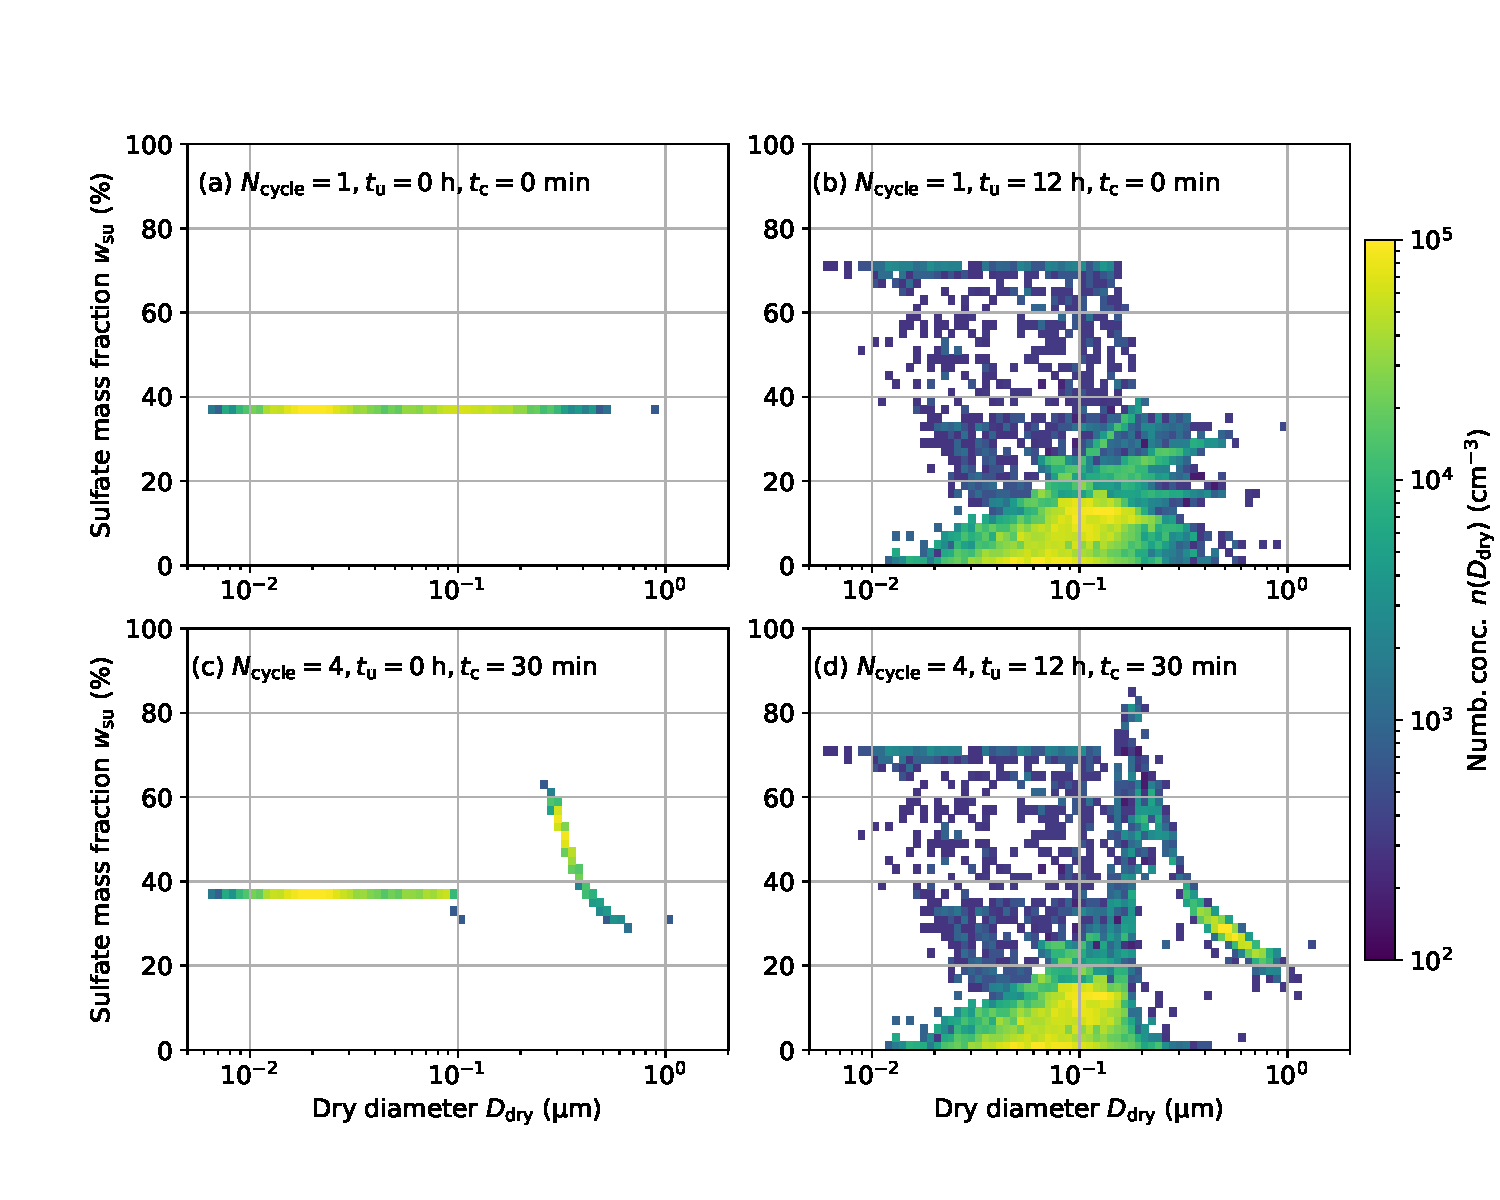
\includegraphics[scale=0.45]{chap3_figs/fig7.pdf}
    \caption{Two-dimensional number concentration distribution
      $n(D_{\rm p}, w_{\rm SO4})$ before cloud processing for (a)
      $t_{\rm u} = 0$~h and (b) $t_{\rm u} = 12$~h
      (high-emission case), (c) population from (a) after four
      cloud cycles, (d) population from (b) after four cloud cycles.}
    \label{fig:su_2d}
\end{figure}


\subsection{Impacts on mixing state and cloud condensation nuclei concentration}
As shown qualitatively in Figure~\ref{fig:su_2d}, cloud processes can
change the diversity and the mixing state of particle populations. In
this section we will quantify these changes for our cases more
precisely using the metrics described in
Chapter~\ref{sec:mixing_state_metrics}. Figure~\ref{fig:bulk_chi}
shows the evolution of $D_\alpha$, $D_\gamma$ and $\chi$ after each of
the four cloud cycles. After the first cloud cycle, the average
particle species diversity $D_\alpha$ increased for aerosols that used
plume hours 0 to 6 as inputs for the cloud parcel simulations. These
populations started with relatively low average particle
diversities. In contrast, $D_\alpha$ decreased for aerosols that used
plume hours 7 to 24 as inputs for the cloud parcel simulations. This
illustrates the fact that the addition of aerosol mass (mainly sulfate
and nitrate) to a subset of particles in a population can lead to a
decrease or increase in average particle diversity, depending on what
the starting point is. When $D_{\alpha}$ was initially low, then
adding secondary species led to more diverse particles, and
$D_{\alpha}$ increased.  This was the case when the aerosol consisted
of different types of freshly emitted aerosol and the particles each
only contained few species in the early stages of the urban plume
simulation. When $D_{\alpha}$ was initially high, adding a small
number of secondary species decreased the diversity, since those newly
added species dominated. This was the case when the aerosol consisted
of aged particles where several species commonly existed within one
particle. This argument applies to both $D_{\alpha}$ and
$D_{\gamma}$. Note that these two cases were contrasted in
\citet{Riemer2013a} as ``Prototypical cases 5 and 6''.  Comparing the
different cloud cycles, we observed that each cloud cycle led to a
less diverse population than the previous cloud cycle.

If $D_{\alpha}$ and $D_{\gamma}$ changed at the same rate, then $\chi$
would remain unchanged by cloud processing. However, here $D_{\alpha}$
generally decreased less than $D_{\gamma}$, and therefore $\chi$
increased for each cloud parcel simulation. The freshly emitted
particles experienced the largest changes, especially for urban plume
particle populations at $t_{\rm u}$ = 2~h, with $\chi$ increasing from
50\% to 83\% after four cycles. One exception was the case using the
aerosol at $t_{\rm u} = 0$~h as input, which was 100\% internally
mixed. The first cloud cycle therefore led to a more external
  mixture (but subsequent cloud cycles led to more internal mixtures),
  however this case is likely not relevant for real atmospheric
  conditions as a completely internal mixture is an idealized
  assumption.

\begin{figure}
    \centering
    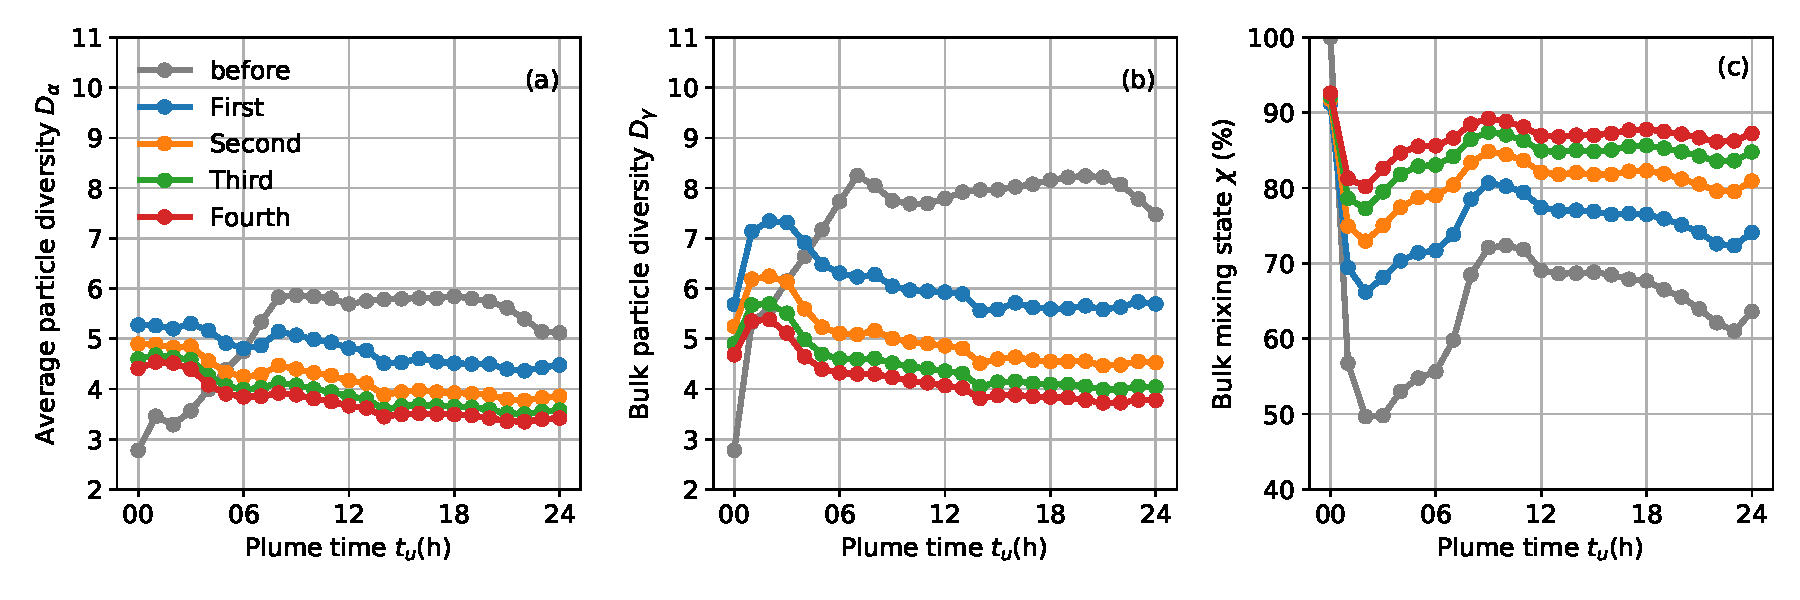
\includegraphics[scale=0.43]{chap3_figs/fig8.pdf}
    \caption{Evolution of average particle diversity $D_{\alpha}$,
      bulk particle diversity $D_{\gamma}$ and bulk mixing state
      $\chi$ ($\%$) at the beginning of cloud cycle 1 and after each
      of the four cloud cycles (high-emission case).}
    \label{fig:bulk_chi}
\end{figure}

Figure~\ref{fig:chi_diagram} graphs the progression of the diversity
metrics in a $D_{\alpha}$- $D_{\gamma}$ diagram using the aerosol at
$t_{\rm u} = 12$~h as input as an example. After each cloud cycle, the
mixing state index moved closer to the diagonal line which indicates a
complete internal mixture ($\chi = 100$\%), with $\chi$ increasing from
69\% to 87\%. However, a complete internal mixture was never reached
because the interstitial aerosol still contributed diversity.

\begin{figure}
    \centering
    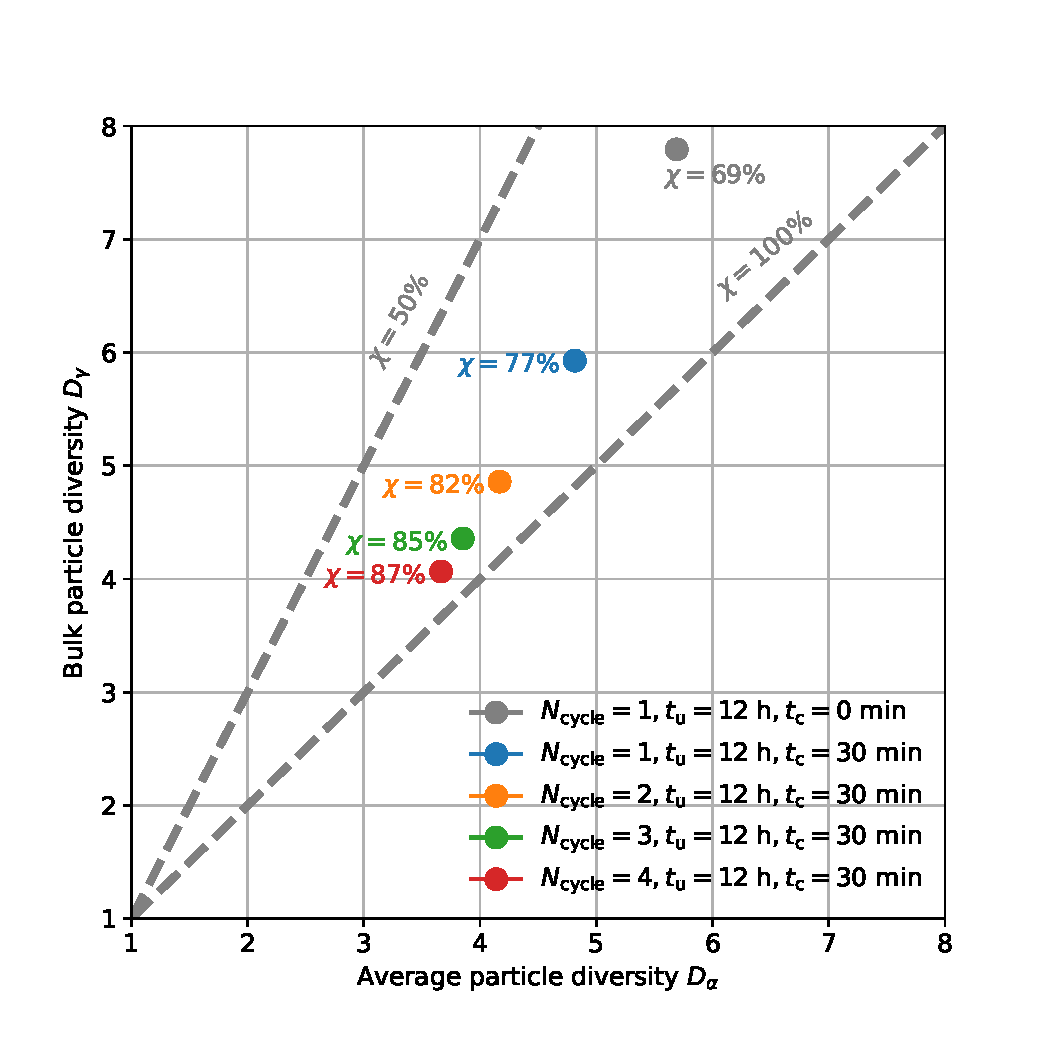
\includegraphics[scale=0.43]{chap3_figs/fig9.pdf}
    \caption{Average particle diversity $D_{\alpha}$ and bulk particle
      diversity $D_{\gamma}$ diagram for the aerosol at $t_{\rm u}$ =
      12~h at the beginning of cloud cycle 1 and after each of the
      four cloud cycles (high-emission case). }
    \label{fig:chi_diagram}
\end{figure}

The change of aerosol mixing state is likely related to the
  fraction of activated particles because only those undergo aqueous-phase chemistry. 
  Figure~\ref{fig:chi-cdnc} compares cloud droplet
  number fraction (number concentration of cloud droplets divided by
  total aerosol concentration at the start of the cloud parcel
  simulation) and change in mixing state for the high-emission case
  and the low-emission case for the first cloud cycle. The cloud
  droplet fraction varied between 10\% and 23\% and between 20\% and
  70\% for the high-emission and low-emission cases, respectively
  (Figure~\ref{fig:chi-cdnc}a). The change in mixing state was indeed
  larger for the low-emission case where $\chi$ reaches values of
  over 90\%  after the first cloud cycle
  (Figure~\ref{fig:chi-cdnc}b). 
\begin{figure}
    \centering
    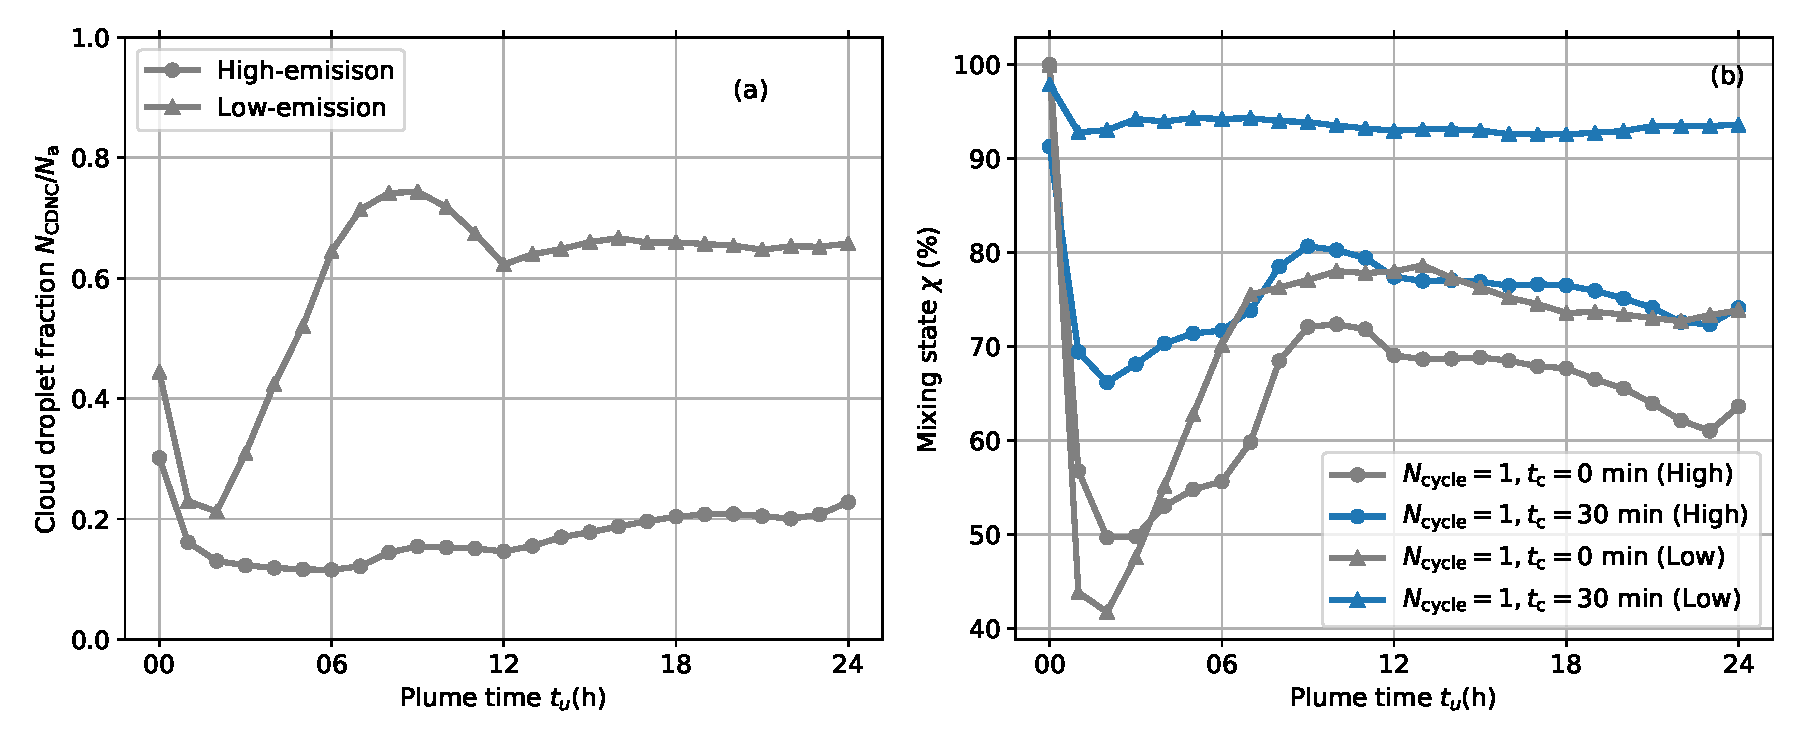
\includegraphics[scale=0.5]{chap3_figs/fig10.pdf}
    \caption{(a) Cloud droplet fraction for the low-emission
        case and the high-emission case (b) Mixing state before
        (grey lines) and after first cloud cycle (blue lines). Circles
        are for the high-emission case and triangles are for
        low-emission case.}
    \label{fig:chi-cdnc}
\end{figure}

CCN properties are determined by particle size and composition. As
illustrated above, the activated particles grew during cloud
processing and attained high hygroscopicity because of the added
ammonium sulfate and ammonium nitrate. Particles with higher
hygroscopicity and larger sizes have smaller critical supersaturation
and activate at lower supersaturation level. Aerosol hygroscopicity has been 
observed to increase significantly because of the
increased ammonium sulfate and ammonium nitrate mass fraction after
cloud processing \citep{Henning2014,Christiansen2020, Saliba2020}.

Figure~\ref{fig:cycle_ccn}a shows the change of CCN spectrum after
each cloud cycle for the high-emission case. As before, the
solid lines indicate the average over the 25 urban plume cases and the
shaded bands show the range of one standard deviation. For
environmental supersaturations larger than 0.15\%, the CCN/CN ratio
remained unchanged after undergoing cloud processing. For
supersaturations lower than 0.15\%, the CCN/CN ratio increased with
the largest increase occurring after the first cloud cycle. This is
expected, since the interstitial aerosol remained unchanged during all
cloud cycles, and only the particles that formed cloud droplets in the
first cycle become progressively more easily activated (i.e. activate
at lower and lower supersaturations).

Figure~\ref{fig:cycle_ccn}b illustrates the changes in CCN number
concentration for the individual plume hours and an environmental
supersaturation of 0.02\%. Before cloud processing, the CCN number
concentrations for all plume hours were less than 30~$\rm cm^{-3}$ at
this supersaturation level. After cloud processing, the CCN/CN
  ratio increased to about 12\%, which translates to a substantial
  increase of absolute CCN number concentration because of the large
  number concentration present in this scenario. For example, the
  population at $t_{\rm u} = 12$~h experienced an increase of CCN
  concentration from 25 to 547~$\rm cm^{-3}$ after the first
  cycle. While the CCN concentrations for supersaturations above the
  value that was reached in the cloud parcel simulations did not
  change, it was sensitive for supersaturations lower than what
  was reached in the cloud parcel simulations.

CCN concentrations for supersaturation thresholds larger than 0.15\%
did not change as a result of aqueous-phase chemistry. This particular
threshold value was determined by the maximum supersaturation obtained
in our cloud parcel simulations, which then governs the subpopulation
of particles that activate. This threshold value is expected to
increase for larger cooling rates which would result in larger maximum
supersaturations (assuming the same aerosol population).

The results look qualitatively similar for the low-emission
  case (Figure~\ref{fig:sup-ccn-low-emi}), however here the supersaturation threshold above
  which the CCN/CN did not change was somewhat larger, consistent
  with the overall higher supersaturations that were reached in the
  cloud parcel simulations (Figure~\ref{fig:max_ss-cycle}a).
  
  \begin{figure}
    \centering
    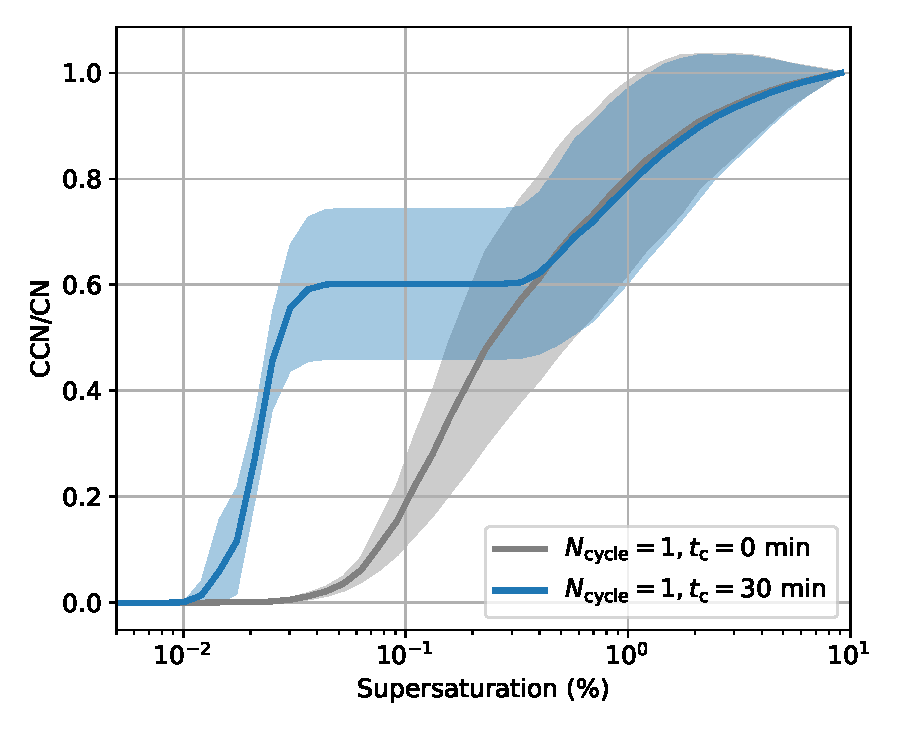
\includegraphics[scale=0.5]{chap3_figs/fig_sup4.pdf}
    \caption{Normalized CCN spectrum before (grey) and after (blue)
      the first cloud cycle for the low-emission case. Solid lines are
      the mean distributions of all 25 cases at each cycle and the
      shaded band represents the 1$\sigma$ range.}
    \label{fig:sup-ccn-low-emi}
\end{figure}

Increases in CCN/CN ratio are generally attributed to both
  increased particle size and (potentially) increased
  hygroscopicity. To disentangle the two factors, we performed a
  sensitivity calculation where we set the hygroscopicity parameter
  $\kappa$ of sulfate, nitrate, and ammonium to 0.1 (representative of
  SOA) for the particles that had experienced cloud processing (i.e.,
  we artificially decreased the hygroscopicity of these particles). The
  modified CCN/CN spectrum is shown in Figure~\ref{fig:sup-new-kappa}. While the addition
  of ammonium sulfate and nitrate increased CCN/CN from 0.01 to 0.11
  for supersaturations lower than 0.04\%, for the sensitivity
  calculation, the ratio only increased to 0.09. That is, only
  increasing the size, but keeping $\kappa$ to a value representative
  of SOA rather than sulfate or nitrate will reduce the effect by
  18\%.
  
  \begin{figure}
    \centering
    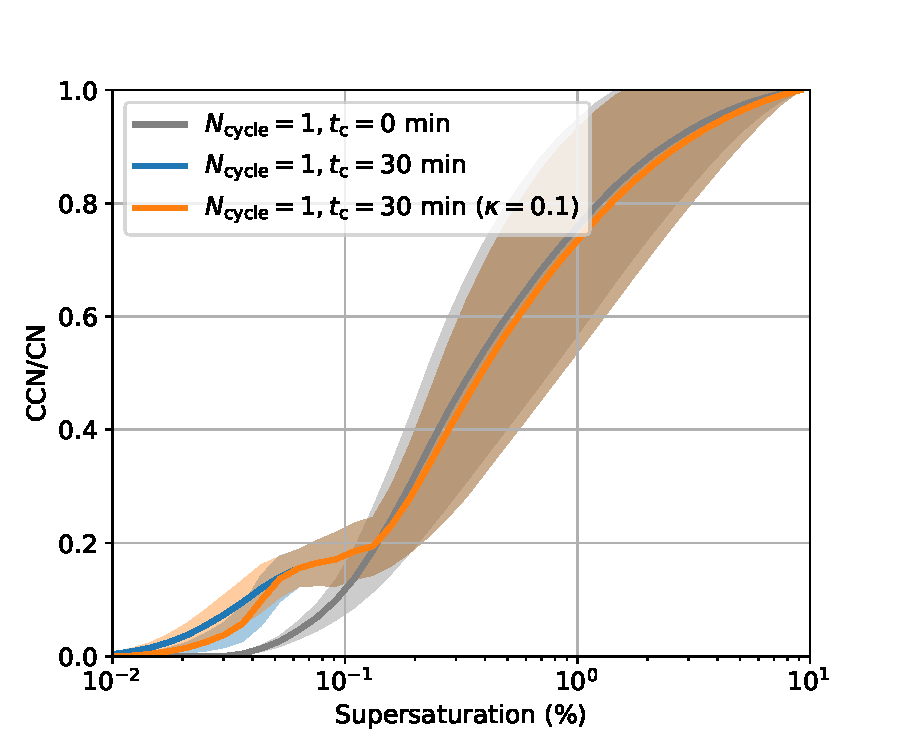
\includegraphics[scale=0.5]{chap3_figs/fig_sup3.pdf}
    \caption{Normalized CCN spectrum before (grey) and after (blue)
      the first cloud cycle (high-emission case). The orange line is
      the CCN spectrum when assuming $\kappa$ = 0.1 for sulfate,
      nitrate and ammonium for the particles that underwent cloud
      processing. Solid lines are the mean distributions of all 25
      cloud parcel cases and the shaded band represents the 1$\sigma$
      range.}
    \label{fig:sup-new-kappa}
\end{figure}

It is worth mentioning that our conclusion that CCN concentration
increased after cloud processing is based on the changes of critical
supersaturation. Previous studies showed that cloud processing can
lead in fact to lower cloud droplet number concentrations in
subsequent cloud cycles. While an increase in particle size due to
aqueous-phase chemistry lowers the critical supersaturation of these
particles, this will suppress the environmental supersaturation in the
subsequent cloud cycle, overall reducing cloud droplet number
concentration \cite{choularton1997effect, feingold2000does,
  romakkaniemi2006influence,
  ivanova2008aerosol,bower1999modelling}. In our study, the maximum
environmental supersaturation indeed decreased in the following cycles
because of the presence of the larger, cloud-processed particles
(Figure~\ref{fig:max_ss-cycle}a), and the cloud droplet concentrations
accordingly decreased in the following cycles
(Figure~\ref{fig:max_ss-cycle}b). This is consistent with
\citet{feingold2000does}, where decreased cloud droplet number
concentration in the subsequent cloud cycles was found for the
environments with larger updraft velocity ($>$ 0.1~$\rm m \, s^{-1}$)
and does not contradict our current findings that processed particles
have a higher activation potential.


\begin{figure}
    \centering
    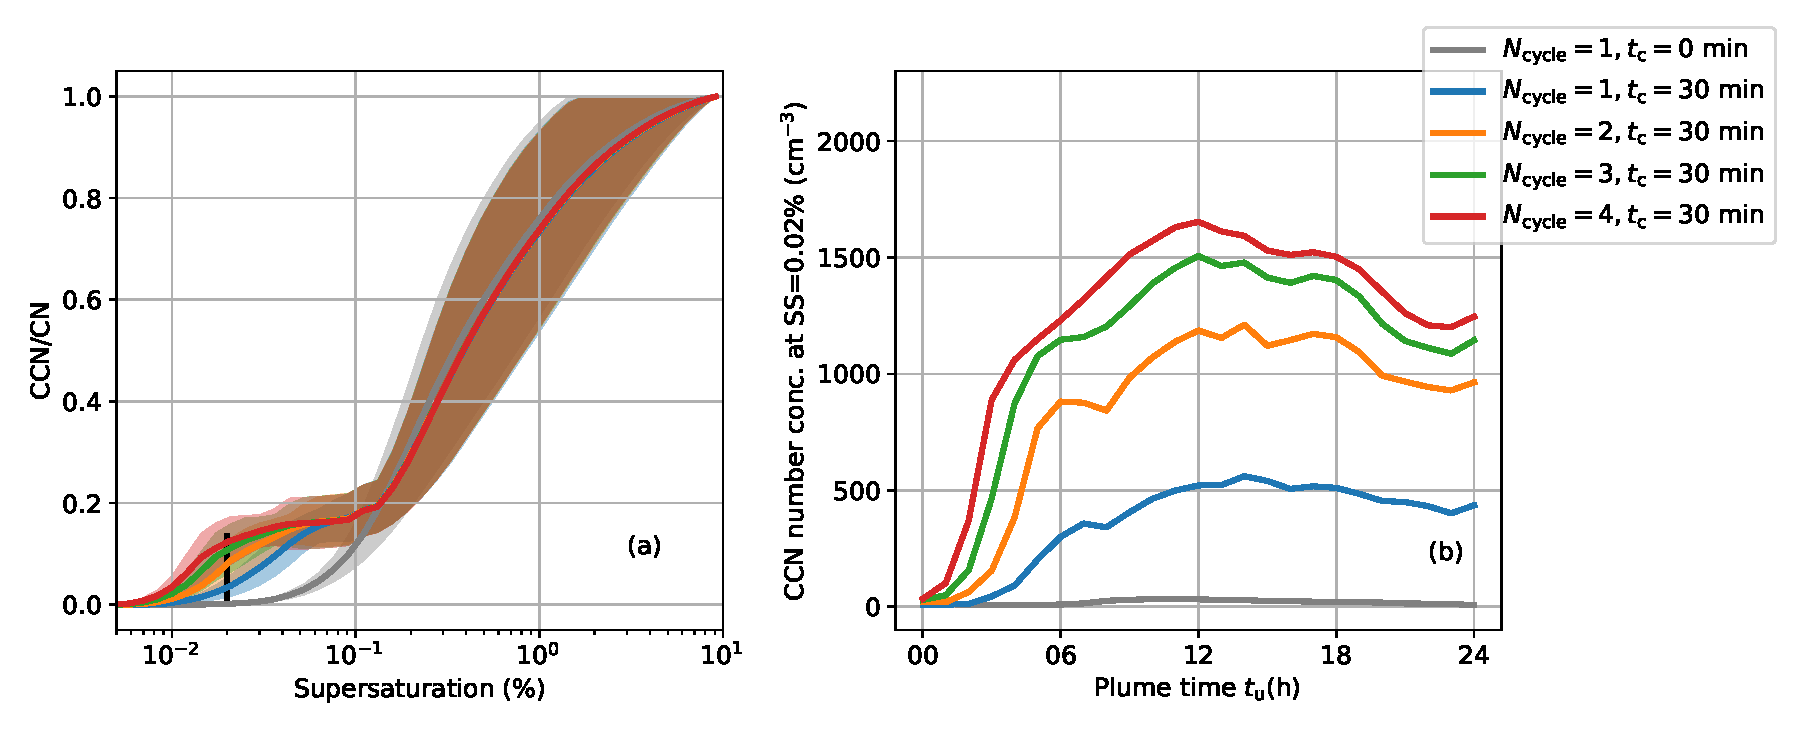
\includegraphics[scale=0.4]{chap3_figs/fig11.pdf}
    \caption{(a) CCN spectrum and (b) CCN number
      concentration at ss = 0.02\% after each of the four cloud
      cycles (high-emission case). Solid lines in (a) are the
      mean distributions of all 25 cases at each cycle and the shaded
      band represents the 1$\sigma$ range. The black line in (a)
      indicates the supersaturation level at 0.02\%, taken here
        as an illustrative example.}
    \label{fig:cycle_ccn}
\end{figure}

\subsection{Effects of in-cloud coagulation on aerosol mixing state} 
\label{sec:coag}

So far we presented results that did not account for coagulation
events within the cloud. We generally include two different
coagulation mechanisms in PartMC, coagulation due to gravitational
differential settling using the coagulation efficiencies according to
\citet{Hall1980}, and Brownian coagulation
\citep{JACOBSON2005}. For the size ranges of droplets in our
  cloud parcel simulations, which is lower than 20~$\rm \mu m$ and not
  large enough to initiate effective collision-coalescence
  \citep{pruppacher2012microphysics}, coagulation due to gravitational
  differential settling was negligible, and therefore we focus the
  discussion on the impact of Brownian coagulation. This is a process
  that is often ignored in aerosol models
  \citep{Pierce2015}. \citet{Pierce2015} report that interstitial
      coagulation in clouds led to a 15\%--21\% decrease of total number
      concentration globally, associated with a global-mean aerosol
      indirect effect of including interstitial scavenging of $+0.5$
      to $+1.3$~$\rm W \, m^{-2}$.


We use the aerosol from $t_{\rm u} = 12$~h as input, since this
population had the largest total number concentration (see
Figure~\ref{fig:urban_plume}a), and so we expected the impacts of
Brownian coagulation to be maximized for this case. Because
coagulation events were simulated stochastically and introduce an
element of randomness into our simulations, we repeated the cloud
parcel simulation three times and report the average and 95\%
confidence interval.

Figure~\ref{fig:coag_num_brown}a compares the number distribution
before and after the first cloud cycle including only aqueous
chemistry and including aqueous chemistry and coagulation. For the
case without Brownian coagulation, the size distribution did not
change for diameters smaller than 0.1~$\rm \mu m$.  With Brownian
coagulation, the number concentration of particles smaller than
0.1~$\rm \mu m$ decreased slightly. The changes in number size
distributions comparing $t_{\rm c} = 0$ min and 30 min are shown
in Figure~\ref{fig:coag_num_brown}b. Brownian coagulation rates were
higher for particle pairs with large diameter difference. Here,
Brownian coagulation depleted the number concentration of particles
between $0.01-0.1$~$\mu$m (the interstitial aerosol). The effects of
aqueous-phase chemistry occurred at larger sizes and moved the
particles from $0.1-0.3$~$\mu$m to $0.3-0.5$~$\mu$m.

\begin{figure}
    \centering
    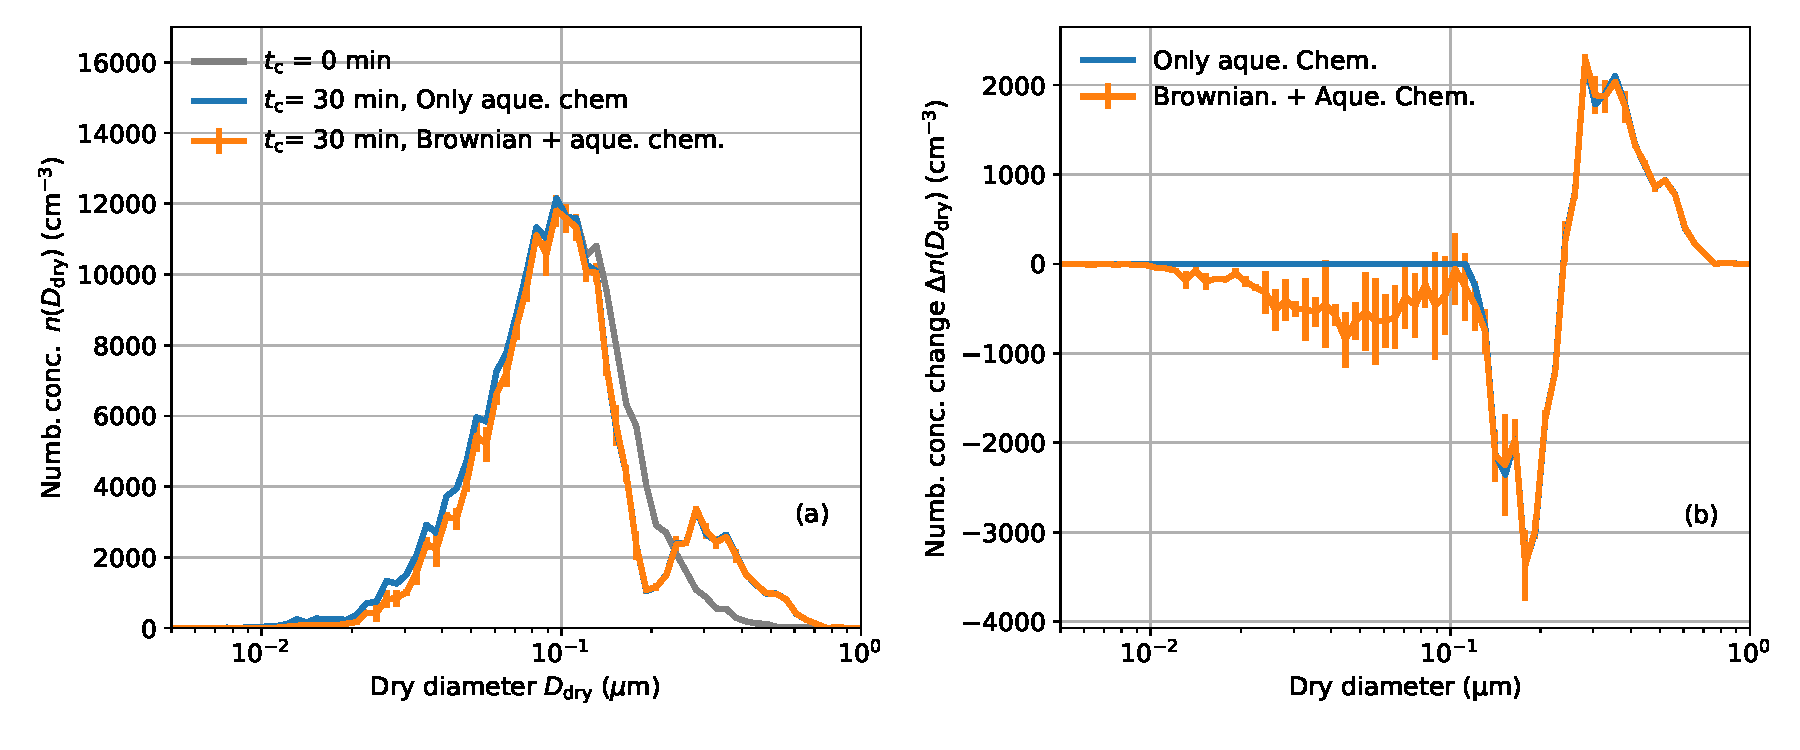
\includegraphics[scale=0.45]{chap3_figs/fig12.pdf}
    \caption{(a) Number distribution at initial condition $t_{\rm c} =
      0$ (grey), at $t_{\rm c} = 30$~min with aqueous chemistry only
      (blue) and at $t_{\rm c} = 30$~min with Brownian coagulation and
      aqueous chemistry (orange) (b) the change of number size
      distribution due to aqueous chemistry and Brownian
      coagulation. The solid orange line is the average of three
      realizations of the cloud parcel model simulation and the error
      bar is the 95$\%$ confidence interval.}
    \label{fig:coag_num_brown}
\end{figure}

Since Brownian coagulation in the cloud mainly affected interstitial
particles, the changes to the CCN spectrum were expected to be small
and should be mainly visible for higher supersaturation levels. As
shown in Figure~\ref{fig:coag_ccn_chi}, the CCN spectrum moved left
only for supersaturation level higher than 0.2$\%$.  For example, with
Brownian coagulation, the CCN/CN ratio increased by 4.1\% from 0.74 to
0.77 at ss = 0.5~$\%$. Figure~\ref{fig:coag_ccn_chi}b shows the change
of CN (total aerosol number concentrations) and CCN concentration in
the simulated 30~minutes. Since the decrease of total aerosol
concentration was larger, this led to the reported increase in CCN/CN
ratio. Including Brownian coagulation caused a decrease of
  total aerosol concentration (by 5.9\%) and of CCN concentration (by
  1.7\%) over the 30-min cloud parcel simulation. We expect this
  effect to be more pronounced for aerosol populations that contain a
  nucleation mode \citep{romakkaniemi2006influence}, which our case did
  not include.

Figure~\ref{fig:coag_ccn_chi}c shows the evolution of $D_{\alpha}$
and $D_{\gamma}$ using output from every minute during the cloud
parcel simulation. The trajectory of the case with Brownian
coagulation was almost identical with the case without Brownian
coagulation, indicating negligible effects of coagulation on mixing
state. Although the differences were small, it was noticeable that
including coagulation does not change $D_{\gamma}$, since the aerosol
bulk mass concentrations were not changed. However, it increased
$D_{\alpha}$, since the average particle diversity increases during
coagulation (archetypical Case~4 in \citet{Riemer2013a}).

\begin{figure}
    \centering
    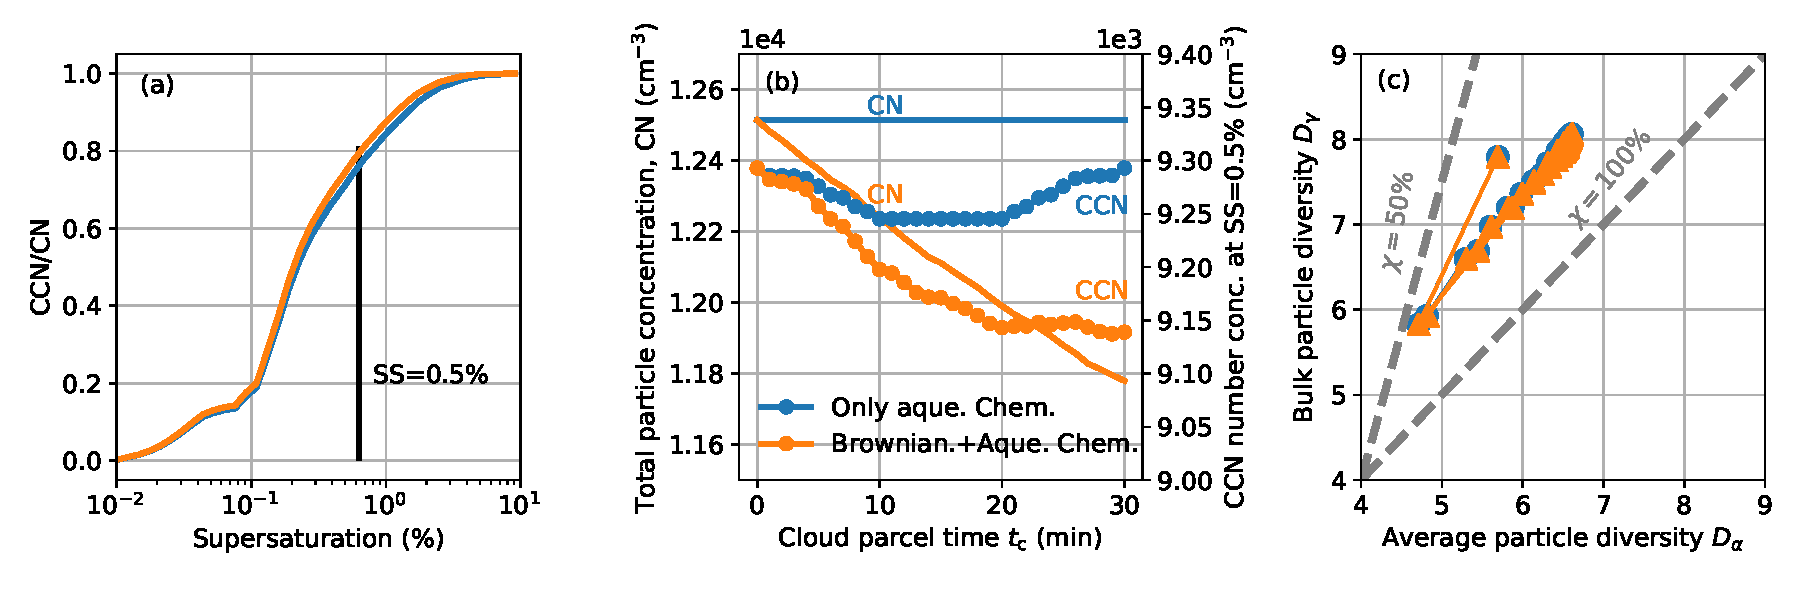
\includegraphics[scale=0.5]{chap3_figs/fig13.pdf}
    \caption{(a) CCN spectrum and (b) total CN and CCN
      concentration at ss = 0.5$\%$ with only aqueous chemistry 
      (blue) and with both Brownian coagulation and aqueous chemistry
      (orange). The vertical line in (a) is for ss = 0.5$\%$, and
      solid and dotted lines in (b) are for total CN and CCN
      concentrations at that level respectively.  (c) Effects of
      coagulation on aerosol mixing state metrics. The points
      correspond to output from every minute during the cloud parcel
      simulation.}
    \label{fig:coag_ccn_chi}
\end{figure}

\subsection{Changes in aerosol scattering and absorption abilities} 
\label{sec:aq-opt}
The changes in aerosol size distribution and composition not only
affect CCN properties, but also aerosol optical properties.  We
analyzed the aerosol optical properties changes in the high-emission
and low-emission cases after the first cloud cycle. As shown in
Figure~\ref{fig:cloud-opt}, all populations have larger scattering
coefficients after cloud processing, consistent with the findings by
\citet{yuskiewicz1999effects} and
\citet{romakkaniemi2006influence}. The enhancement was more obvious
for the low-emission case, where the median scattering coefficient
increased from $1.3\times10^{-4}$ to 10.9$\times 10^{-4}$~\unit{m^{-1}}.

\begin{figure}[H]
    \centering
    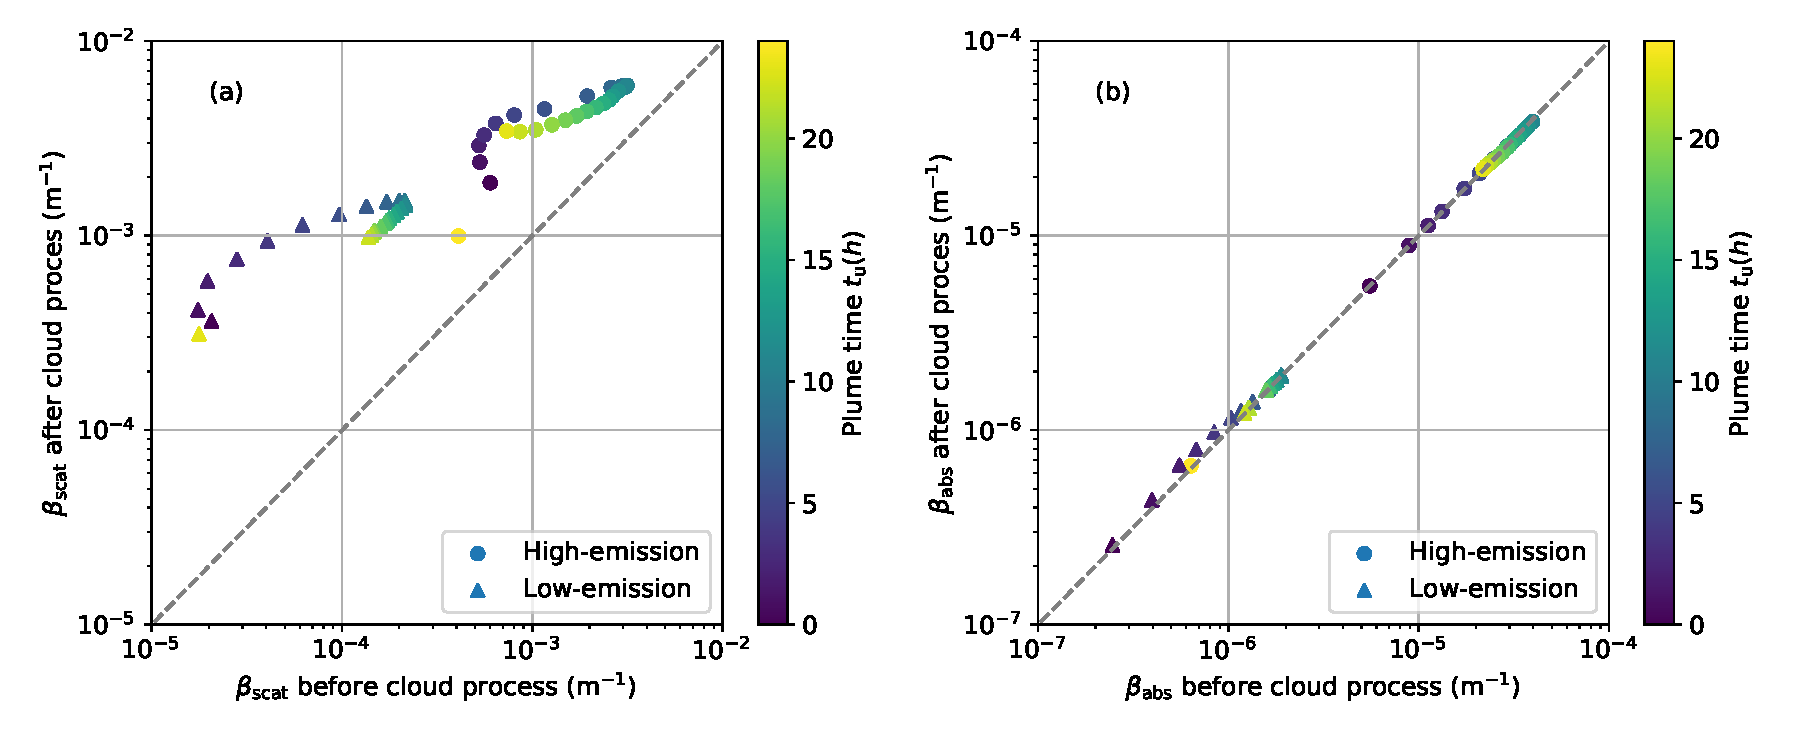
\includegraphics[scale=0.5]{chap3_figs/fig14.pdf}
    \caption{Optical properties befor and after cloud processing. (a)
      Scattering coefficient $\beta_{\rm scat}$. (b) Absorption
      coefficient $\beta_{abs}$. Circles are for high-emission case and
      triangles are for low-emission case. The color indicates the plume
      hour. }
    \label{fig:cloud-opt}
\end{figure}

The absorption coefficients do not change after cloud processing.
This can be explained by the fact that only few BC-containing
particles were activated. As shown in Figure~\ref{fig:bc-2d}, in both
the high-emission and low-emission case, the activated particles are
contain less than 10\% of BC. Particles with larger BC fraction are
smaller particles and they were not affected by cloud processing.
 
 \begin{figure}[H]
    \centering
    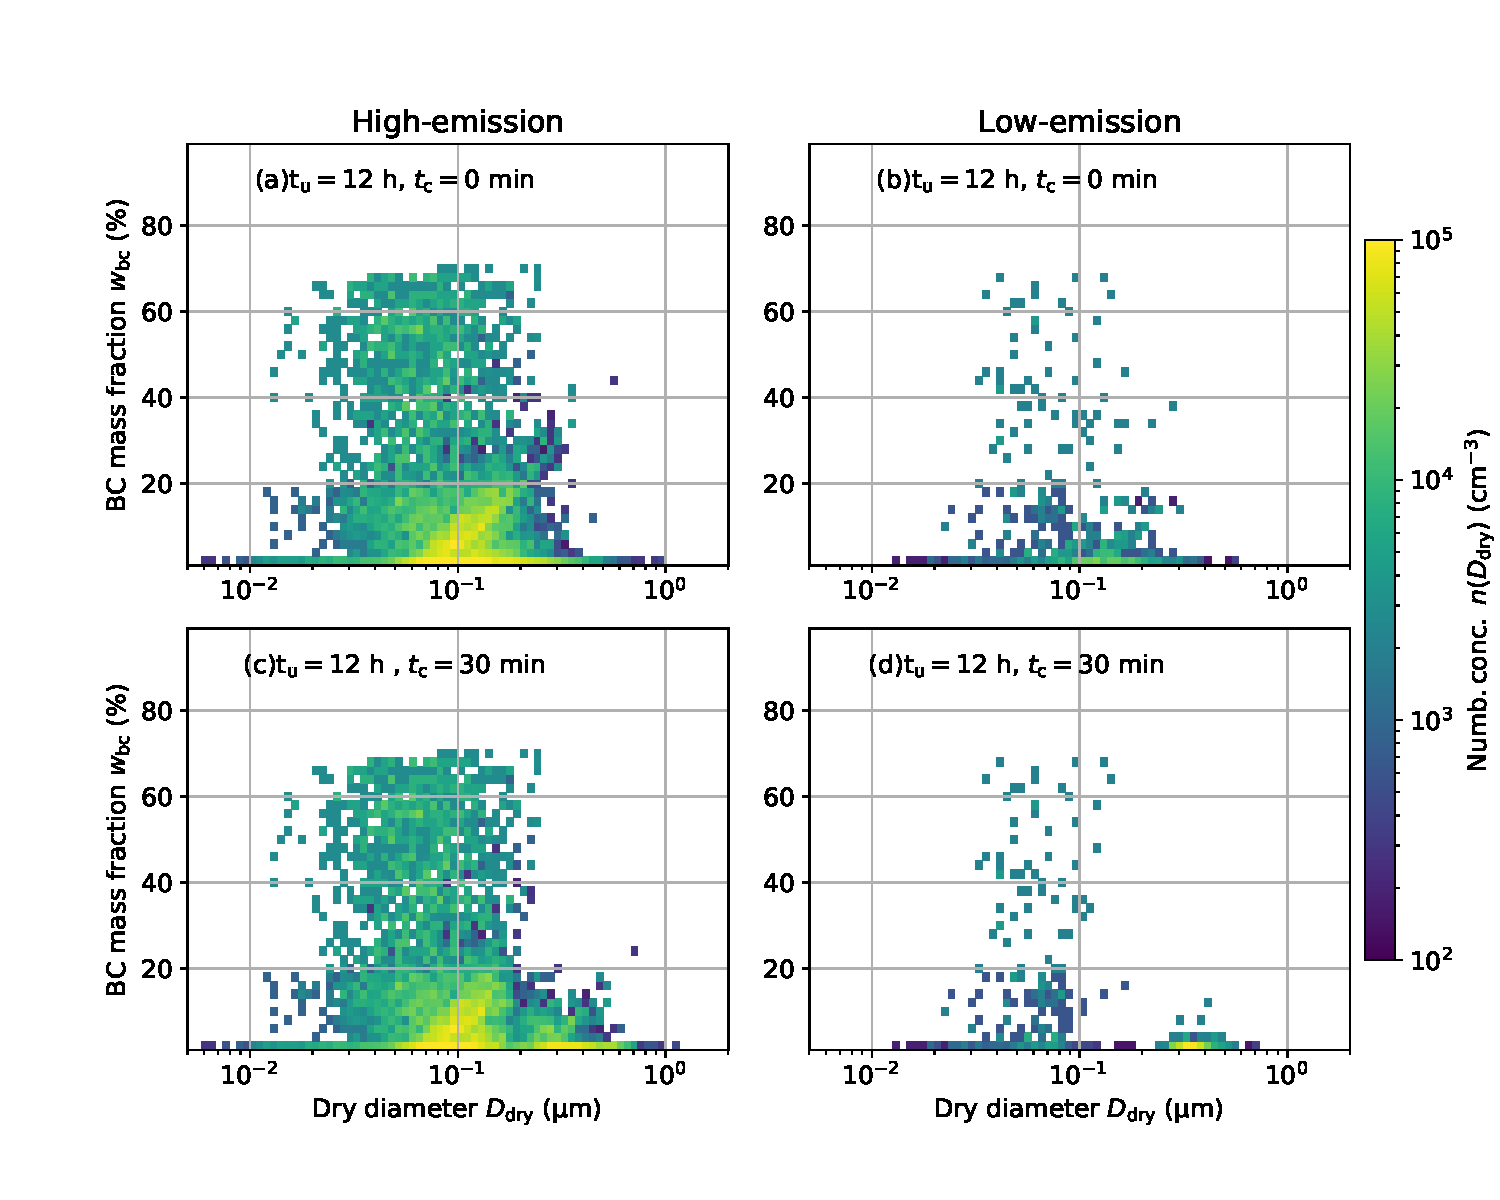
\includegraphics[scale=0.5]{chap3_figs/fig15.pdf}
    \caption{Two-dimensional number concentration distribution
      $n(D_{\rm p}, w_{\rm bc})$ before cloud processing (a,b) and
      after cloud processing (c,d) for aerosol populations from
      $t_{\rm u}$=12~\unit{h}.  The left column is for high-emission
      case and the right column is for low-emission case.}
    \label{fig:bc-2d}
\end{figure}

%
\section{Conclusions}
\label{sec:conclusions}
In this study, we investigated the impact of in-cloud aqueous-phase
chemistry on aerosol mixing state. Using the particle-resolved model
PartMC-MOSAIC, we generated particle populations of different aerosol
mixing states from urban plume simulations representing
polluted conditions. We used these as inputs for 30-min cloud parcel
simulations that included the reduced CAPRAM 2.4 aqueous-phase
chemistry mechanism. Each cloud parcel simulation was driven by the
same temperature profile, with decreasing temperature during the first
10 min, constant temperature during the second 10 min, and increasing
temperature during the third 10 min. While the cloud parcel
simulations were simplified in that we assumed adiabatic conditions,
our results are a first step towards investigating aerosol-cloud
interactions within a particle-resolved framework that allows for
representing aerosol mixing state without simplifying assumptions.

Coming back to the questions that we posed in the introduction, we
conclude the following. We quantified changes in mixing state as a result of in-cloud
processes using the diversity metrics $D_{\alpha}$ (average particle
diversity) and $D_{\gamma}$ (bulk aerosol diversity) and the mixing
state index $\chi$. The aqueous-phase chemistry processes had an
``equalizing effect'' on the diversity metrics, meaning that
$D_{\alpha}$ and $D_{\gamma}$ increased due to aqueous-phase chemistry
when the initial values were low and decreased when the initial values
were high. The first condition applied for plume time hours 0--6 in
our high-emission scenario, when fresh emissions dominated
which tend to be of low diversity, consistent with observational
findings \citep{Healy2014}. Adding secondary species to the activated
particles increased the diversities. The opposite was the case when
$D_{\alpha}$ and $D_{\gamma}$ values started out high, which applied
to plume time hours 7--24, when the plume was aged. Here, adding
secondary species to the activated particles decreased the
diversities.

Whether the overall population became more or less internally mixed
depended on the relative changes in $D_{\alpha}$ and $D_{\gamma}$. For
most populations in our study, aqueous-phase chemistry led to a more
internally mixed aerosol. For example, for the population of plume
hour $t_{\rm u}=12$~h, $\chi$ increased from 69\% to 77\% after the
first cloud cycle, and to 87\% after the fourth cloud cycle. However,
a completely internal mixture was not achieved under the conditions
investigated here, since only a portion of the aerosol population
activated and the remaining interstitial aerosol always contributed
diversity to the population. An exception was the case of plume hour
$t_{\rm u} = 0$, when the initial aerosol population was completely
internally mixed. In this case, aqueous-phase chemistry caused the
population to become more externally mixed.

The change in mixing state index $\chi$ due to cloud processing
  depended also on the fraction of particles that formed cloud
  droplets. In our high-emission case, this fraction remained below
  23\% and $\chi$ did not exceed 90\% even after the fourth cloud
  cycle. In contrast, for the low-emission case, the fraction of
  activated particles ranged between 20\% and 75\%, and $\chi$
  increased to over 90\%  after the first cloud cycle.

The size changes after cloud processing led to significant changes to
aerosol microphysical properties. With ammonium nitrate and ammonium
sulfate added to the activated particles, after the cloud evaporated,
the activation potential of the resuspended aerosol particles
increased remarkably for low supersaturation thresholds. For example,
the CCN concentration for particles from the high-emission case
  at $t_{\rm u}=12$~h and supersaturation level 0.02\% increased by a
factor of 20 from 30~$\rm cm^{-3}$ to 547~$\rm cm^{-3}$ after the
first cloud cycle. For subsequent cloud cycles, the increase was
smaller and by the fourth cycle, it was only 8.8\%.

The effects of coagulation due to gravitational settling were
negligible in our simulations. This can be explained by the fact that
the cloud droplets did not grow large enough for gravitational
settling to take over as main coagulation mechanisms. Brownian
coagulation occurred mainly between the interstitial particles at
around 0.1~$\rm \mu m$ and cloud droplets at 10~$\rm \mu m$. The
number concentration reduction caused by coagulation was up to
5.8~$\%$ in the cases considered while the CCN concentration was
reduced by less than 2\%. This therefore resulted in an increase of
the CCN/CN ratio for supersaturations higher than 0.2\%. The change in
aerosol mixing state caused by coagulation was negligible. It should
be noted that our simulations did not take into account the impact of
phoretic or turbulence effects on coagulation, which could modify the
efficiency of in-cloud coagulation.

We also found that cloud processing enhanced particle
  scattering due to particle growth, and the effects are more profound
  for high-emission case, with the median scattering coefficient
  increasing from $1.3\times10^{-4}$ to 10.9$\times
  10^{-4}$~\unit{m^{-1}}. For the scenarios considered here, the
  particle absorption did not change, which can be explained by the
  fact that the cloud droplets only contained small amounts of BC.
%%%%%%%%%%%%%%%%%%%%%%%%%%%%%
%%%%%%%%%Chapter 4%%%%%%%%%%%
%%%%%%%%%%%%%%%%%%%%%%%%%%%%%

\chapter{Quantifying the effects of mixing state on aerosol optical properties}
This chapter develops a framework to systematically quantify the
aerosol optical value errors introduced by simplified aerosol representation.  I first
introduce the processes to create reference and sensitivity
scenarios. Then, I present the errors in aerosol absorbing and
scattering properties introduced by internal mixture assumptions used
by sectional aerosol models. The work is in preparation for
\textit{Atmospheric Chemistry and Physics}.

\label{chap4}
\section{Introduction}  %% \introduction[modified heading if necessary]
Aerosol particles scatter and absorb incoming solar radiation, thereby
impacting the global radiative balance and surface temperatures
\citep{mitchell1971effect, charlson1992climate, yu2006review,
  winker2010calipso, oikawa2013study, subba2020recent}. Black carbon
(BC), commonly emitted from combustion, has a direct radiative forcing
of $+0.9$~\unit{W\,m^{-2}}, which is next only to $\rm CO_2$
\citep{bond2013bounding, gustafsson2016convergence} in its warming
impact. At the same time, the overall global average aerosol direct
radiative forcing in the clear-sky environment is
$-1.9$~\unit{W\,m^{-2}} because of the presence of other
non-absorbing aerosol species, which exert a cooling impact
\citep{bellouin2005global}.

Radiative effects of aerosols depend on their optical properties,
which, as a whole, are determined by the individual particles that the
aerosol consists of. As observed in field campaigns, particles are
mixtures of inorganic and organic species, and exhibit significant
spacial and temporal variation in their abundance and composition
\citep{zhang2007ubiquity, bzdek2012single, LASKIN2006260}, with
considerable diversity in composition existing within individual
aerosol populations. The topic of this chapter is to quantify the importance
of diversity in composition for aerosol optical properties.

Aerosol composition impacts aerosol optical properties for several
reasons. First, aerosol species differ in their complex refractive
index. While inorganic species and many organic species have a purely
real refractive index (i.e. only scatter radiation) for wavelength of
visible sunlight, black carbon and some organic carbon species have a
non-zero imaginary part of the refractive index and hence also absorb
radiation \citep{corbin2018brown, Esteve2014, cappa2019light}.
Second, aerosol species differ in their hygroscopicity. This governs
aerosol water uptake in a humidified environment, which is important
for scattering \citep{MichelFlores2012, Zieger2013, Titos2014,
  Titos2016}.

Lastly, the arrangement of the different aerosol species within a
particle is important for determining their scattering and
absorption. For mixed particles without strongly absorbing species,
i.e. BC, a volume-mixing rule can be used to calculate the refractive
index of the entire particle. When the particle contains BC, assuming
a core-shell configuration was proven to be more accurate
\citep{Bond2006} (still assuming sphericity as particle shape). The
absorption enhancement of BC-containing particles due to their
non-absorbing coatings has been widely investigated
\citep{Moffet2009,Liu2017,wu2020light, Fierce2020}. Taking the
non-shperical shapes of BC-containing particles into account
complicates matter considerably since Mie calculations cannot be
applied and more sophisticated optical models need to be used, which
are computationally much more expensive. By using the Discrete Dipole
Approximation model, \citet{scarnato2013effects} found
BC-NaCl mixtures absorption coefficients enhancement is higher for
compact BC particles completely embedded in NaCl than for lacy BC
particles.

To understand the importance of aerosol composition in calculating
aerosol optical properties, it is useful to define the term aerosol
mixing state, that is, the distribution of aerosol species among the
particles in a population \citep{Riemer2009,Riemer2013a}. Aerosol
mixing state in the ambient atmosphere ranges between the two
idealized extremes of an external mixture on the one hand, where
different aerosol species reside in different particles, and an
internal mixture on the other hand, where all particles consist of the
same mixture of species. Aerosols close to emission sources tend to be
more (although not completely) externally mixed \citep{Bondy2018,
  Rissler2014}. After emission, aging processes, such as coagulation
between particles and condensation of gas species on the particles,
transform aerosol populations towards more internal mixtures
\citep{Healy2014, Liu2013, Zaveri2010a}.

Aerosol mixing state is challenging to represent in 3D chemical
transport models, which usually rely on simplifying assumptions for
computational efficiency. These assumptions then determine how aerosol
optical properties are calculated. Optical properties are here
understood by three widely-used parameters: absorption cross section,
scattering cross section and asymmetry parameter \citep{Majdi2020}.
For example, many 3D models use a modal approach to represent aerosol,
such as The Community Multiscale Air Quality Modeling System (CMAQ)\citep{Binkowski2007,
  Appel2017} and Modal Aerosol Module (MAM)\citep{Liu2012}. The modes are externally mixed from each other,
whereas within each mode, the aerosol is assumed to be internally
mixed. For BC-containing modes, sphericity and a core-shell
configuration are assumed, so that Mie calculations can be applied to
calculate optical properties. \citet{Fierce2016} found that neglecting
the diversity in coating thickness for BC-containing particles (a
result of the internal mixture assumption) leads to overestimatd
absorption enhancement by up to 200\%. Another approach is the
sectional model representation, which tracks size-resolved
composition, but not particle composition diversity within a certain
size, such as TwO-Moment Aerosol Sectional (TOMAS) and the GLObal
Model of Aerosol Processes (GLOMAP)\citep{kodros2018size,
  spracklen2005global}.  Still, mixing state assumptions need to be
invoked for each size bin. The importance of mixing state was
quantified through optical closure studies.  Using the measured
aerosol size distributions and composition collected over East China
Sea, \citet{koike2014case} found that neglecting BC mixing state can
lead to uncertainty level of $-$18\% to $+$9\% in calculated
absorption aerosol optical depth.

The uncertainties in optical properties introduced by mixing state
assumptions had been also widely evaluated through model sensitivity
studies.  Using the AQMEII-2 model inter-comparison framework,
\citet{Curci2015} quantified the sensitivity of aerosol optical
properties to several parameters, including aerosol mixing state and
size distribution, and they found that aerosol mixing state is the
dominant factor introducing uncertainties, explaining 30--35\% of the
aerosol optical depth and single scattering albedo (SSA)
uncertainty. \citet{kodros2018size} found that the direct radiative
forcing (DRF) can vary from $-1.65$ to $-1.34$ W $\rm m^{-2}$ over the
pan-Arctic region in spring depending on the assumption of internal or
external mixture. The variation is similar when the assumptions are
used to calculate DRF at the top of atmosphere
\citep{ma2012aerosol}. An open questions of these sensitivity studies
is that no benchmark simulation exists that represents the real mixing
state, and therefore the importance of mixing state can only be
assessed based on differences between varied idealized assumptions. By
applying a detailed particle-resolved benchmark model,
\citet{Fierce2017} found that simple mixing state assumption can
result in an artificial redistribution of BC mass between particles
and lead to errors in absorption. The redistribution was further
confirmed to be the main source for the discrepancies between the
simulated and experimentally-determined particle optical properties
\citep{Fierce2020}.

The goal of this study is to systematically quantify the errors in
optical properties due to simplified assumptions for mixing state,
here quantified with the mixing state index $\chi$
\citet{Riemer2013a}. A similar framework was used to quantify the
error in CCN concentration \citep{Ching2017}, showing that CCN error
can range from $-40$\% to 150\% when assuming the aerosol was
internally mixed. The error depended on supersaturation level that CCN
concentrations were evaluated at, and also aerosol mixing state. In this
chapter, we want to answer: Given the aerosol mixing state, what is
the error in aerosol optical values when assuming internal mixture and
what are the reasons?

The chapter is structured as follows: Model description, scenario design and
the definition of metrics are given in
Chapter~\ref{sec:methods}. Chapter~\ref{sec:dry-case} shows the relation
between the errors in aerosol scattering and absorption and mixing
state for dry aerosol populations, and Chapter~\ref{sec:wet-case}
further analyzes the errors for the aerosol populations at different
levels of ambient relative humidity. The errors in single scattering
albedo and its implications for aerosol direct radiative forcing are
analyzed in Chapter~\ref{sec:ssa}. Chapter~\ref{sec:conclusion}
summarizes the main findings.

\section{Model description, scenario libraries and metrics }
\label{sec:methods}
\subsection{Particle-resolved model PartMC-MOSAIC}
The model used to generate the particle populations for this study is
the particle-resolved model PartMC-MOSAIC. A comprehensive description
of the model can be found in \citet{Riemer2009} for PartMC and in
\citet{Zaveri2008} for MOSAIC. PartMC is a Lagrangian box model which
tracks the evolution of particles in a fully-mixed computational
volume. The processes of emission, coagulation and dilution are
simulated stochastically. Gas-phase chemistry and gas-aerosol
partitioning are incorporated by coupling with the deterministic model
MOSAIC. Specifically, MOSAIC uses the carbon bond based mechanism
CBM-Z for gas-phase photochemical reactions \citep{zaveri1999new},
MTEM for calculating electrolyte activity coefficients in aqueous
inorganic mixtures and MESA for calculating the phase states of the
particles \citep{zaveri2005computationally}. The secondary organic
aerosol (SOA) treatment follows the SORGAM scheme.  Aerosol water
uptake is calculated using Zdanovskii‐Stokes‐Robinson (ZSR) method
\citep{Zaveri2008, zdanovskii1948new,stokes1966interactions} based on
the composition of the inorganic portion of the particles.  By this
method, organic species are treated as hydrophobic, and do not
contribute to water uptake. The impact of this assumption on optical
properties was quantified by \citet{nandy2021water}, 
where they found errors in single scattering ability can be over 6\% 
if neglecting organic compounds water uptake. 

\subsection{Scenario library design}
Following the strategy in \citet{zheng2021estimating} and
\citet{hughes2018machine}, we created a scenario library of a large
number of PartMC-MOSAIC simulations, for this study with a focus on
the aging of carbonaceous aerosol. To produce particle populations
with a wide range of compositions and mixing states, we varied the
model input parameters within the ranges shown in
Table~\ref{tab:input}. We used Latin hypercube sampling
\citep{mckay2000comparison} to create input parameter combinations for
a total of 100 model simulations. The simulation time for each
simulation was 24 hours beginning at 6 am local time with hourly
output. This yielded a total of 2500 particle populations. All
scenarios were run with 10\,000 computational particles.  To create
aerosol initial conditions with realistic mixing states, we adopted the
approach described in \citet{zheng2021estimating}: We carried out a first set of
simulations, starting with the aerosol initial concentrations set to
zero for all simulations (the ``initial runs''). We then repeated the
same set of simulations, but replaced the aerosol initial condition
with a randomly sampled population from the initial runs (the
``restart runs''). For the analysis in this chapter, we only used the
results from the restart runs.

\begin{table}
\centering
\caption{Baseline and range for the input variables}
\label{tab:input}
\begin{tabular}{ c c c  }
	\hline
	Input parameters  & Baseline & Range  \\
	\hline
	\multicolumn{3}{c}{Enviroment Variables} \\
	\hline
    Relative humidity (RH)&&[0.1, 1) or [0.4, 1) \\
    Latitude & &($70^o$S, $70^o$N) or ($90^o$S, $90^o$N)  \\
    Day of year & & [1, 365]\\
    Temperature & & Based on latitude and day of year\\
    \hline
    \multicolumn{3}{c}{Gas emission rates ($\rm mol$ $\rm m^{-2}$ $\rm s^{-1}$)} \\
    \hline
    Sulfur dioxide ($\rm SO_2$)&8.5$\times$ $10^{-9}$&[0-200\%] \\
    Nitrogen dioxide ($\rm NO_2$) &3.0$\times$ $10^{-9}$&[0-200\%]\\
    Nitrogen oxide ($\rm NO$) &5.7$\times$ $10^{-8}$& [0-200\%]\\
    Ammonia ($\rm NH_3$)&8.9$\times$ $10^{-9}$&[0-200\%] \\
    Carbon oxide (CO)&7.8$\times$ $10^{-7}$& [0-200\%]\\
    Methanol (CH3OH)&2.3$\times$ $10^{-10}$& [0-200\%]\\
    Acetaldehyde ($\rm ALD2$) &1.7$\times$ $10^{-9}$&[0-200\%] \\
    Ethanol (ANOL) &5.3$\times$ $10^{-9}$& [0-200\%]\\
    Acetone (AONE) &7.8$\times$ $10^{-10}$&[0-200\%]\\
    Dimethyl sulfide (DMS) &3.8$\times$ $10^{-11}$&[0-200\%] \\
    Ethene (ETH) &1.8$\times$ $10^{-8}$&[0-200\%] \\
    Formaldehyde (HCHO) &4.1$\times$ $10^{-9}$&[0-200\%] \\
    Isoprene (ISOP) &2.4$\times$ $10^{-10}$&[0-200\%] \\
    Internal olefin carbons (OLEI) &5.9$\times$ $10^{-9}$&[0-200\%]\\
   Terminal olefin carbons (OLET)&5.9$\times$ $10^{-9}$& [0-200\%]\\
   Paraffin carbon (PAR)) &1.7$\times$ $10^{-7}$&[0-200\%] \\
   Toluene (TOL) &6.1$\times$ $10^{-9}$&[0-200\%] \\
   Xylene (XYL) &5.6$\times$ $10^{-9}$&[0-200\%] \\
    \hline
    \multicolumn{3}{c}{Carbonaceous aerosol emission (single mode)} \\
    \hline
    Geometric mean diameter ($D_g$) &&[25, 250]~\unit{nm}\\
    Geometric standard deviation of diameter ($\sigma_g$) && [1.4, 2.5]\\
    BC/OC mass ratio && [0, 100\%] \\
    Particle emission flux && [0, 1.6$\times$ $10^{7}$] $\rm m^{-2}$ $\rm s^{-1}$ \\
	\hline
\end{tabular}
\end{table}

\subsection{Optical properties calculations}
We calculated the optical properties of the particle populations using
Mie calculations \citep{Zaveri2010a}. These properties included the
asymmetry parameter $g$, scattering cross section $\sigma_{\rm scat}$
and absorption cross section $\sigma_{\rm abs}$ for each
particle. Particles were assumed to be spherical, and when BC was
present, a core-shell configuration was assumed, with BC as the core
and non-BC species as the shell. In PartMC-MOSAIC, each chemical
species was assigned a refractive index and the values were the same 
as \citet{Zaveri2010a}, as listed
in Table~\ref{tab:refrc_inex}. The shell refractive index of the
particle was the volume average of all the shell species, including
aerosol water. The absorptivity of brown carbon has been of great
interest in recent years \citep{corbin2018brown, cappa2019light},
however, this was not considered in the current work. We used the
wavelength $\lambda$ of 550~\unit{nm} for our analysis.
\begin{table}
	\centering
	\caption{Refractive indices of aerosol species at $\lambda$ =
          550~\unit{nm}}
	\label{tab:refrc_inex}
	\begin{tabular}{ c  c  c }
		\hline 
		Compounds & Refractive index\\
       \hline
       $\rm H_2SO_4$ & 1.43 \\
       $\rm {(NH_4)}_2SO_4$ & 1.52 \\
       $\rm (NH_4HSO_4$ & 1.47 \\
       $\rm NH_4NO_3$ & 1.5 \\
       $\rm H_2O$ & 1.33 \\
       $\rm BC$ & 1.82 + 0.74$i$ \\
       $\rm SOA$ & 1.45  \\
       $\rm POA$ & 1.45 \\       
       \hline
	\end{tabular}
\end{table}
In PartMC-MOSAIC, all particles are tracked individually in a
well-mixed computational volume, and we obtain the ensemble
optical property values by summing over all particles in the
volume. The ensemble scattering, absorption and extinction
coefficients at wavelength $\lambda$ are given as 

\begin{align}
\centering
    \label{eq:opt-cal1}
    \beta_{\rm scat}(\lambda) &= \sum\limits_i^{N}\sigma_{{\rm scat},i}(\lambda)n_i,\\
    \label{eq:opt-cal2}
    \beta_{\rm ext}(\lambda)  &= \sum\limits_i^{N}\sigma_{{\rm scat},i}(\lambda)n_i, \\
    \label{eq:opt-cal3}
    \beta_{\rm abs}(\lambda)  &= \beta_{\rm ext}(\lambda) - \beta_{\rm scat}(\lambda),
\end{align}

where $i$ is the particle index, $n_i$ is the number concentration
associated with particle $i$ and $N$ is the number of computational
particles in the population. We determined the optical properties of
all particle populations of our scenario libraries using these
equations.

\subsection{Quantifying the impact of mixing state through composition-averaging}
To quantify the impacts of mixing state on aerosol optical properties,
we employed the strategy of ``composition-averaging'' similar to
\citet{Ching2016}. The technique is shown conceptually in
Fig.~\ref{fig1:scen}. For each population in our reference scenario
library, we averaged the dry particle compositions within prescribed
size bins. We chose eight size bins between 0.039 and 10~\unit{\mu m},
consistent with the bin structure of the sectional aerosol module
MOSAIC used in WRF-Chem \citep{fast2006evolution}.

The composition-averaging procedure preserves the bulk mass
concentration of each species, the total number concentration, and the
particle diameters within each bin. It changes the composition so that
each bin becomes internally mixed, however the composition can vary
between bins. This mimics the assumption frequently made in sectional
models, namely that each size bin contains an internally mixed
aerosol. It is worth mentioning that PartMC-MOSAIC represents
particles outside the MOSAIC bin range, especially for the lower
boundary, and we used an extra bin (bin 0) to preserve the total
number and mass concentrations.

The changes of two important parameters for aerosol optical properties
due to composition-averaging are illustrated in Fig.~\ref{fig1:scen},
BC mass fraction and the real part of the refractive index. In the
reference case, a wide range of BC mass fractions exists within the
same size bin. After composition-averaging, all particles within a
size bin have the same BC mass fraction.  Since composition-averaging
preserves the particle diameters, BC and other species are
redistributed so that all particles within a size bin obtain the same
mass fractions. Specifically, if a particle has lower BC mass fraction
than the average level in the same size bin, BC is added to this
particle from those with higher BC content. The coating species are
also redistributed after composition-averaging which causes the
refractive index of the coating to change. Hence, comparing optical
properties before and after composition-averaging in the dry
population $P_1$ isolates the impact of mixing state on aerosol
optical properties.

%\textcolor{red}{Should we say something about sensitivity to size
%  bins? Could we repeat the calculations for 1 bin (complete internal
%  mixture) and a lot of bins, and report how overall error changes
%  (not include any figures)?}

Since the aerosol water content plays an important role for aerosol
optical properties, we further calculated water uptake for the
reference populations and for the composition averaged populations for
50\% ($P_2$) and for 90\% ($P_3$) relative humidity, respectively.  At
$\rm RH = 50$\%, depending on the exact composition, some particles
take up water, and at $\rm RH = 90$\%, most particles take up water,
except particles that only contain hydrophobic species, such pure
black carbon or primary organic carbon. Note that while the dry
aerosol mass was conserved by the composition-averaging procedure, the
water content was re-calculated after composition-averaging and could
change compared to the reference population. We will discuss the
impact of composition-averaging for dry conditions in
Chapter~\ref{sec:dry-case} and the impact of water uptake in
Chapter~\ref{sec:wet-case}.

\begin{figure}
\centering
\begin{subfigure}{0.8\textwidth}
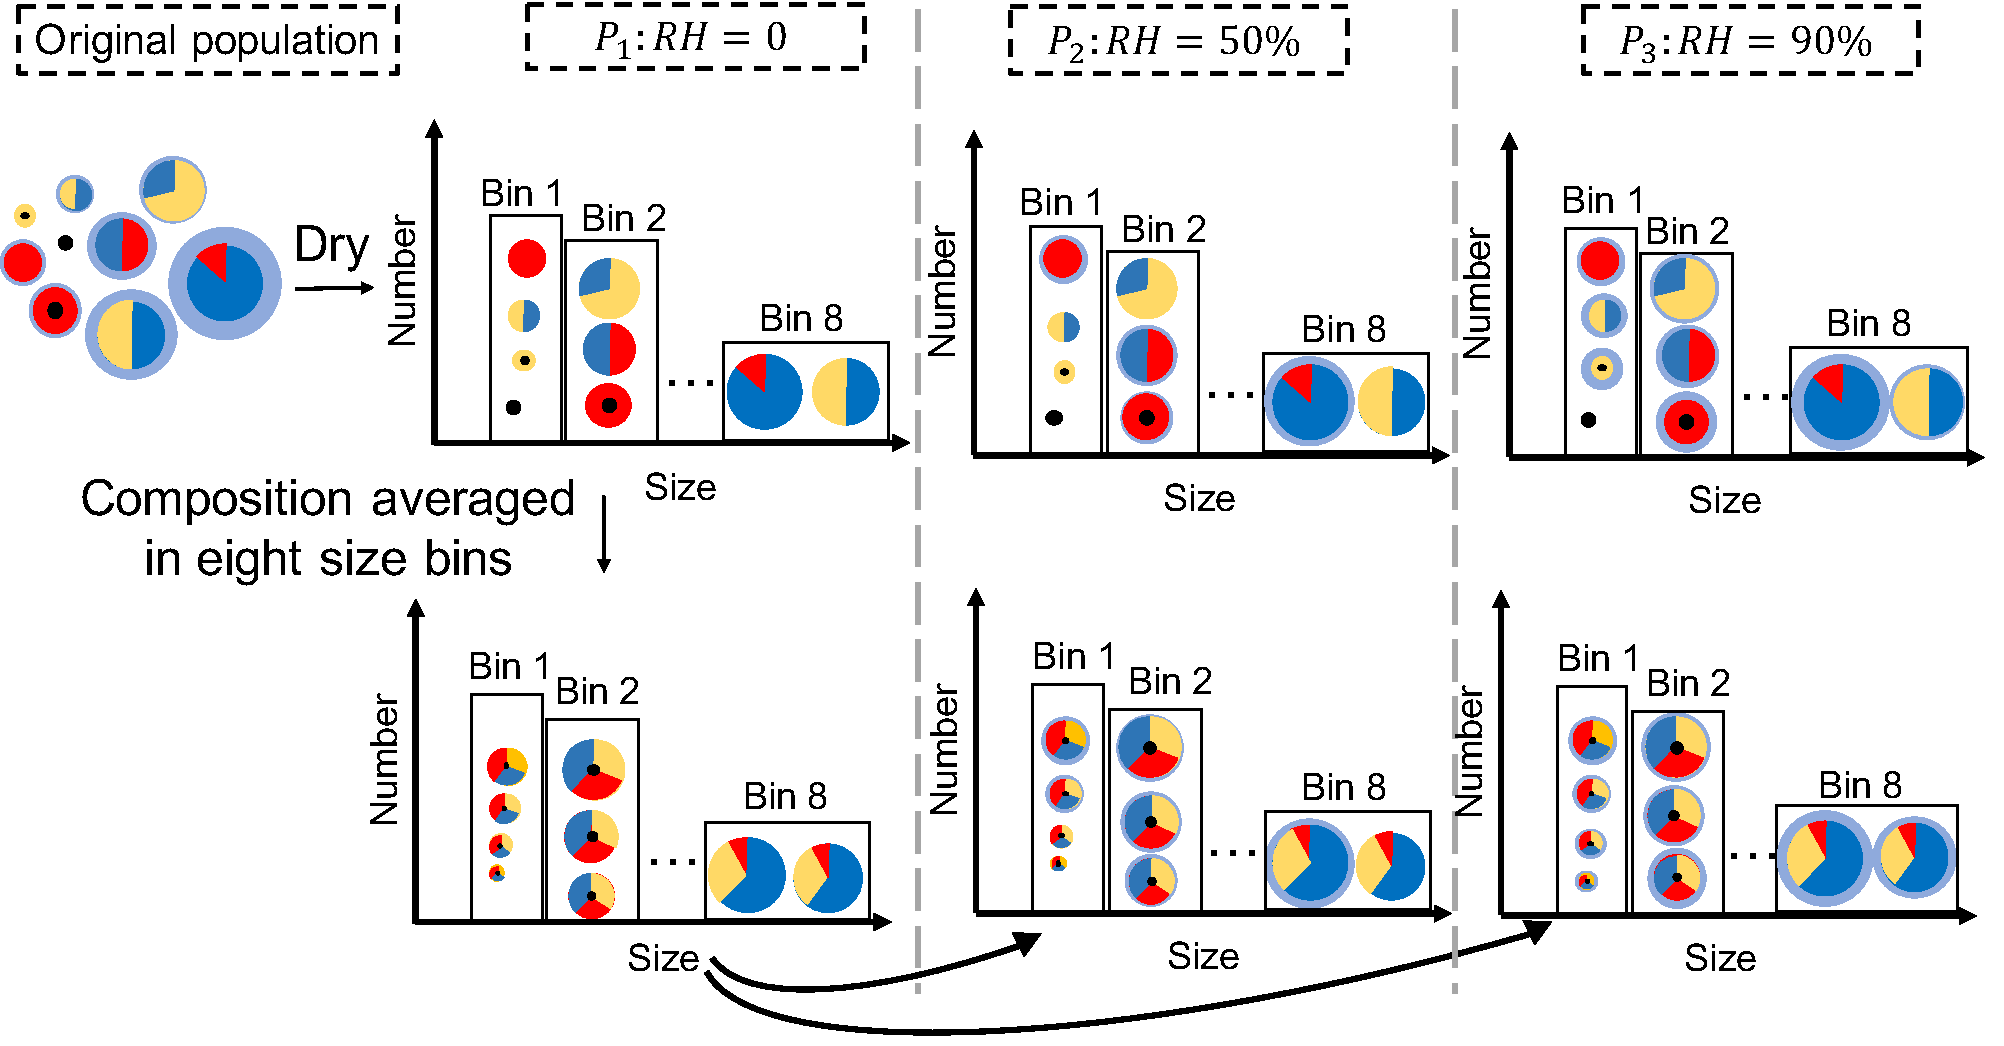
\includegraphics[scale=0.45]{chap4_figs/fig1.pdf}
\end{subfigure}
\begin{subfigure}{0.8\textwidth}
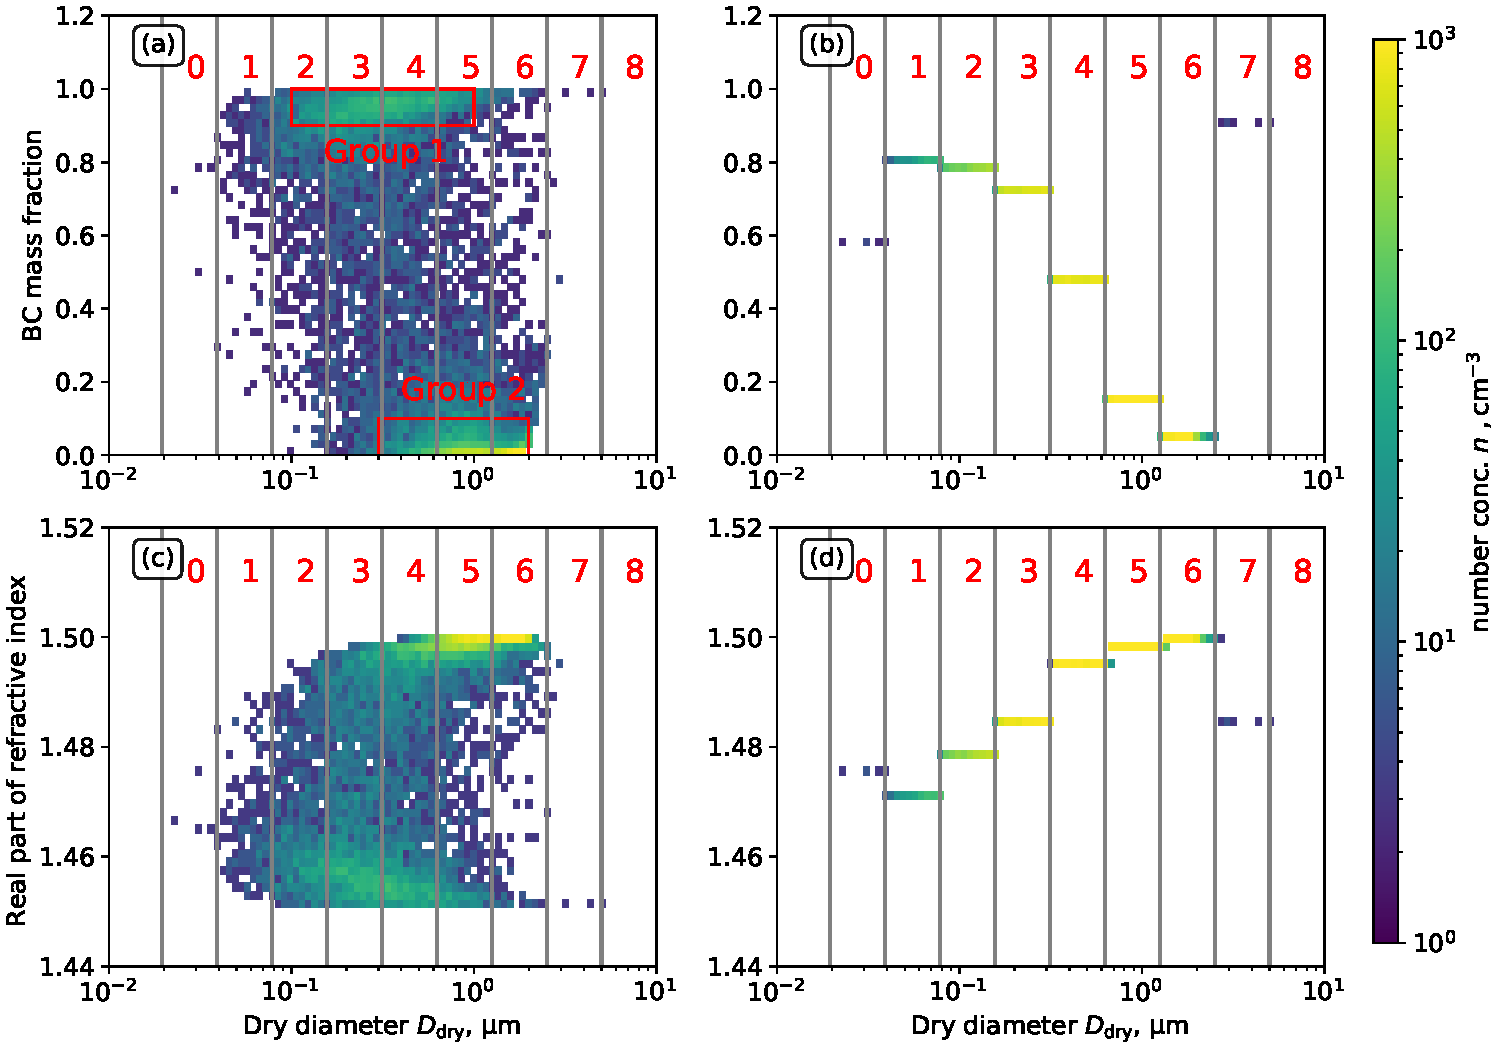
\includegraphics[scale=0.56]{chap4_figs/fig2.pdf}
\end{subfigure}
\caption{Conceptual framework of composition-averaging. In the top
  panel, aerosol species and water are shown with different
  colors. Water is in light blue, BC is in black, and other colors are
  for the other chemical species. The middle and bottom panels are the
  two-dimensional distributions of BC mass fraction and real part of
  refractive index for a particle population from reference (a,c) and
  sensitivity (b,d) scenario. The plots are colored by number
  concentration.  Red numbers and grey lines represent the size bin
  ranges, comparable to the bin structure used in WRF-Chem. Bin 0 is
  the extra bin to preserve the total number concentration. The two
  red rectangles are for the analysis in
  Chapter~\ref{sec:dry-case}. This population is taken from scenario
  76 at 1~h, with $\chi$=36\%.}
\label{fig1:scen}
\end{figure}

\subsection{Mixing state metrics}
We quantified the optical properties error introduced by simplified
mixing state representation by using the metrics developed by \citet{Riemer2013a}. These metrics
include the single-particle diversity $D_i$, the average particle
species diversity $D_\alpha$ and bulk population species diversity
$D_\gamma$. For a population with $N$ particles, total mass $\mu$ and
$A$ species, we can calculate those metrics from the total mass of
particle $i$, $\mu_i$, total mass of species $a$ in the population,
$\mu^a$, and mass of species $a$ in particle $i$, $\mu_i^{a}$, for $i$
= 1, ..., $N$ and $a$ = 1,..., $A$. Mass fraction of species $a$ in
particle $i$, $p_i^a$, mass fraction of particle $i$ in the
population, $p_i$ and mass fraction of species $a$ in the population,
$p^a$ are given by
\begin{equation}
\label{eq:frac}
\begin{split}
    p_i^a = \frac{\mu_i^a}{\mu_i},\;\;\;p_i = \frac{\mu_i}{\mu},\;\;\;p^a = \frac{\mu^a}{\mu}.
\end{split}
\end{equation}

Single particle diversity $D_i$ describes the effective species number
in each particle, and is defined as

\begin{equation}
D_i = \prod_{a=1}^A({p}_i^a)^{-p_i^a}.
\end{equation}
For particles containing the same number of species type, particle
diversity $D_i$ reaches its maximum when species are present in equal
amounts. Based on $D_i$, we can construct $D_\alpha$ and $D_\gamma$,
which describes the average effective species number in each particle
and bulk population respectively:
\begin{align}
\centering
 \label{Dalpha}
 D_\alpha & = \prod_{i=1}^N (D_i)^{p_i},\\
 \label{Dgamma}
 D_\gamma &= \prod_{i=1}^A(p^a)^{-p^a}.  
\end{align}

Finally, the mixing state metric $\chi$ is defined as the affine ratio
of $D_\alpha$ and $D_\gamma$:
\begin{equation}
\chi = \frac{D_\alpha - 1}{D_\gamma - 1}.
\end{equation}
The values of $\chi$ vary between 0\% to 100\%. When $\chi$ = 0\%, it
indicates that the population is fully externally mixed and each
particle only contains one species. The population is internally mixed
when $\chi$ = 100\%, and all particles have the same species mass
fractions.  For this work, our focus is the optical properties of the
particles. Differing from the traditional chemical species mixing
state index, we grouped the aerosol species by absorbing and
non-absorbing species and defined a new index, $\chi_{\rm opt}$. It
still ranges between 0\% to 100\% and signifies the degree to which
absorbing and non-absorbing species are mixed. Since we only consider
two (surrogate) aerosol species, the maximum value of $D_i$,
$D_\alpha$ and $D_\gamma$ is 2. For the remainder of the chapter, we
will refer to this index simply as $\chi$.

Within our ensemble or aerosol populations, some were found with
higher species concentrations than what would be expected in the
ambient atmosphere. We applied upper thresholds to eliminate those
which were calculated as the sum of $\rm 75^{th}$ percentile and 1.5
IQR (interquartile range) for each of the aerosol species. After this
procedure, 1809 out of 2500 populations were used for error analysis.
Figure~\ref{fig2:sce_overview} shows the range of bulk chemical
species concentrations, mixing state index, and optical properties
within the selected scenario library. The simulated aerosol bulk
species mass concentration in the library covered a wide range of
urban conditions (Fig.\ref{fig2:sce_overview}a), and the values were
comparable to the measurements in different locations
\citep{jimenez2009evolution,lanz2010characterization}. As for the
distribution of mixing state, most populations had a mixing state
index $\chi$ larger than 40\%, with a median value of 85\%.  The fact
that $\chi$ values smaller than 40\% did not occur in our scenario
library was consistent with the notion that BC rarely existed in a
completely external mixture. It is frequently co-emitted with organic
carbon, which form internal mixtures at the time of
emission. Additionally, in urban environments, BC ages quickly,
forming internal mixtures with secondary species.
Figure~\ref{fig2:sce_overview}c shows that the single scattering
albedo (SSA) was larger than 0.4 for all populations, with a median
value of 0.88. While SSA values lower than 0.5 can be considered
extremely low (4\%), most populations (72\%) are with SSA larger than
0.85, which is consistent with fine mode SSA observations from AERONET
\citep{levy2007global}.

\begin{figure}
	\centering
	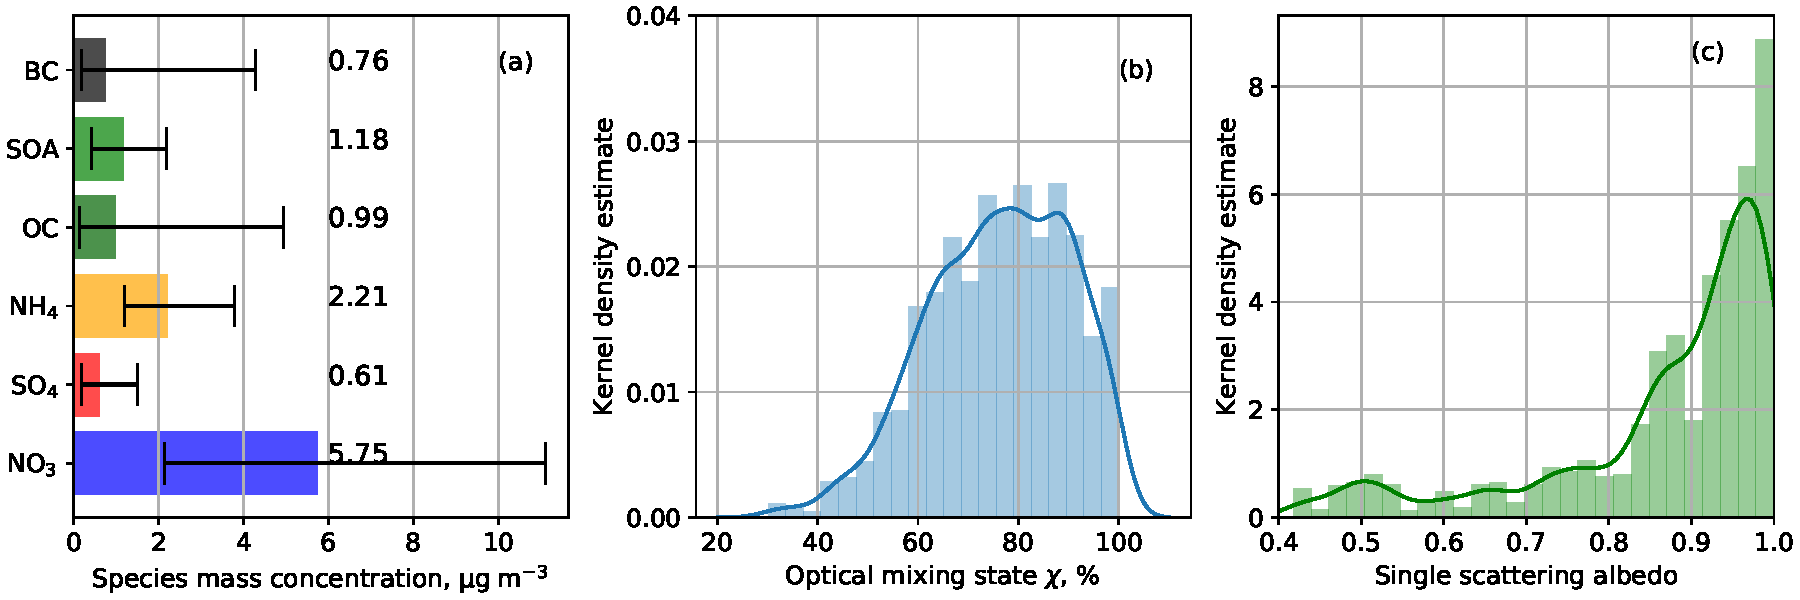
\includegraphics[scale=0.5]{chap4_figs/fig3.pdf}
	\caption{Distribution of (a) bulk species concentration, (b)
          optical mixing state $\chi$ and (c) SSA in the scenario
          libraries. Error bars in (a) are for $\pm$1 IQR and numbers
          are the median species concentration.}
	\label{fig2:sce_overview}
\end{figure}

The following sections describe the error introduced by
composition-averaging assumptions and how the error depends on mixing
state. Similar to the methods used by \citet{Ching2017}, we stratified
the populations by optical mixing state index $\chi$. In order to
isolate the impacts of mixing state (in the sense of how the chemical
species except for aerosol water are distributed across the
population) from the impacts of water uptake, we first analyzed the
results for the dry population scenarios $P_1$. This quantified the
effects of chemical species redistribution caused by simplified mixing
state assumption used in sectional models. Particles were partially or
fully deliquescent in scenarios $P_2$ and $P_3$, and these populations
will be further analyzed in Chapter~\ref{sec:wet-case} to quantify the
water uptake effects on aerosol optical properties resulting
from internally mixing hygroscopic and hydrophobic species.

\section{Errors in aerosol absorptivity and scattering for dry particles}
\label{sec:dry-case}
We quantified the errors in aerosol optical properties by comparing
the values of reference and composition-averaged
populations. The relative error for the aerosol
populations was calculated as
\begin{equation}
  \epsilon(v,\chi) = \frac{v'(\chi) - v(\chi)}{v(\chi)}, 
\end{equation}
where $v$ can be SSA, $\beta_{\rm abs}$ or $\beta_{\rm scat}$, and
$\chi$ is mixing state index. We analyzed the error of these three
parameters separately.

\subsection{Errors in aerosol absorptivity due to composition-averaging}
Absorption was overestimated universally after composition-averaging,
and, as expected, the error was higher for more externally-mixed
populations (low $\chi$ values), with $\epsilon(\beta_{\rm abs})$
reaching up to +70\% for $\chi$ of 30\%
(Fig.\ref{fig3:abs-error}). Each dot represents a particle population
from the scenario library. As shown in the box plot inset, the mean
overestimation was 18\% and the maximum reached over 80\%. The figure
further contains information of BC bulk mass concentration and
relative BC core size changes, which are the two main factors in
determining absorptivity \citep{Bond2006a}, as represented by circle
size and color, respectively. The relative BC core size change is
defined as
\begin{equation}
    \displaystyle \Delta{D^{\rm core}}=\frac{\sum_{i=1}^{N} n_i {D_i^{\rm core}}' - \sum_{i=1}^{N} n_i {D_i^{\rm core}}}{\sum_{i=1}^{N} n_i D_i^{\rm core}},
\end{equation}
where $i$ is the particle index, $n_i$ and $D_i^{\rm core}$ are the
associated number concentration and core diameter in the reference
scenario, and ${D_i^{\rm core}}'$ is the core diameter in the
sensitivity scenario. It is interesting to note that $\Delta
D^{\rm core}$ is always positive, that is, the average core diameter
after composition-averaging is larger than the average core diameter
before composition-averaging. This is a result of particle mass being
a convex function of particle diameter (assuming spherical
particles). Calculating the new core diameters after composition
averaging will therefore always lead to on-average larger core
diameters than averaging the core diameters before composition
averaging.

The decreasing error with increasing $\chi$ can be explained by the
magnitude of $\Delta{D^{\rm core}}$. Evidently, composition-averaging
caused larger changes of BC core sizes when the populations were more
externally mixed. For example, for $\chi=30$\%, the change in core
sizes was as large than +25\%, while for $\chi=95$\%, the change in
core sizes was less than 5\%.  We also noticed a wide range of errors
for populations with $\chi$ between 60 and 70\%, i.e., partially
internally-mixed populations. In fact, the highest overestimation of
82\% was reached at $\chi= 63$\%. As indicated by the circle size,
these populations contained very little BC (0.01~\unit{\mu g\,m^{-3}})
and even small changes in core sizes can lead to large relative errors
in volume absorption coefficient.
\begin{figure}
	\centering
	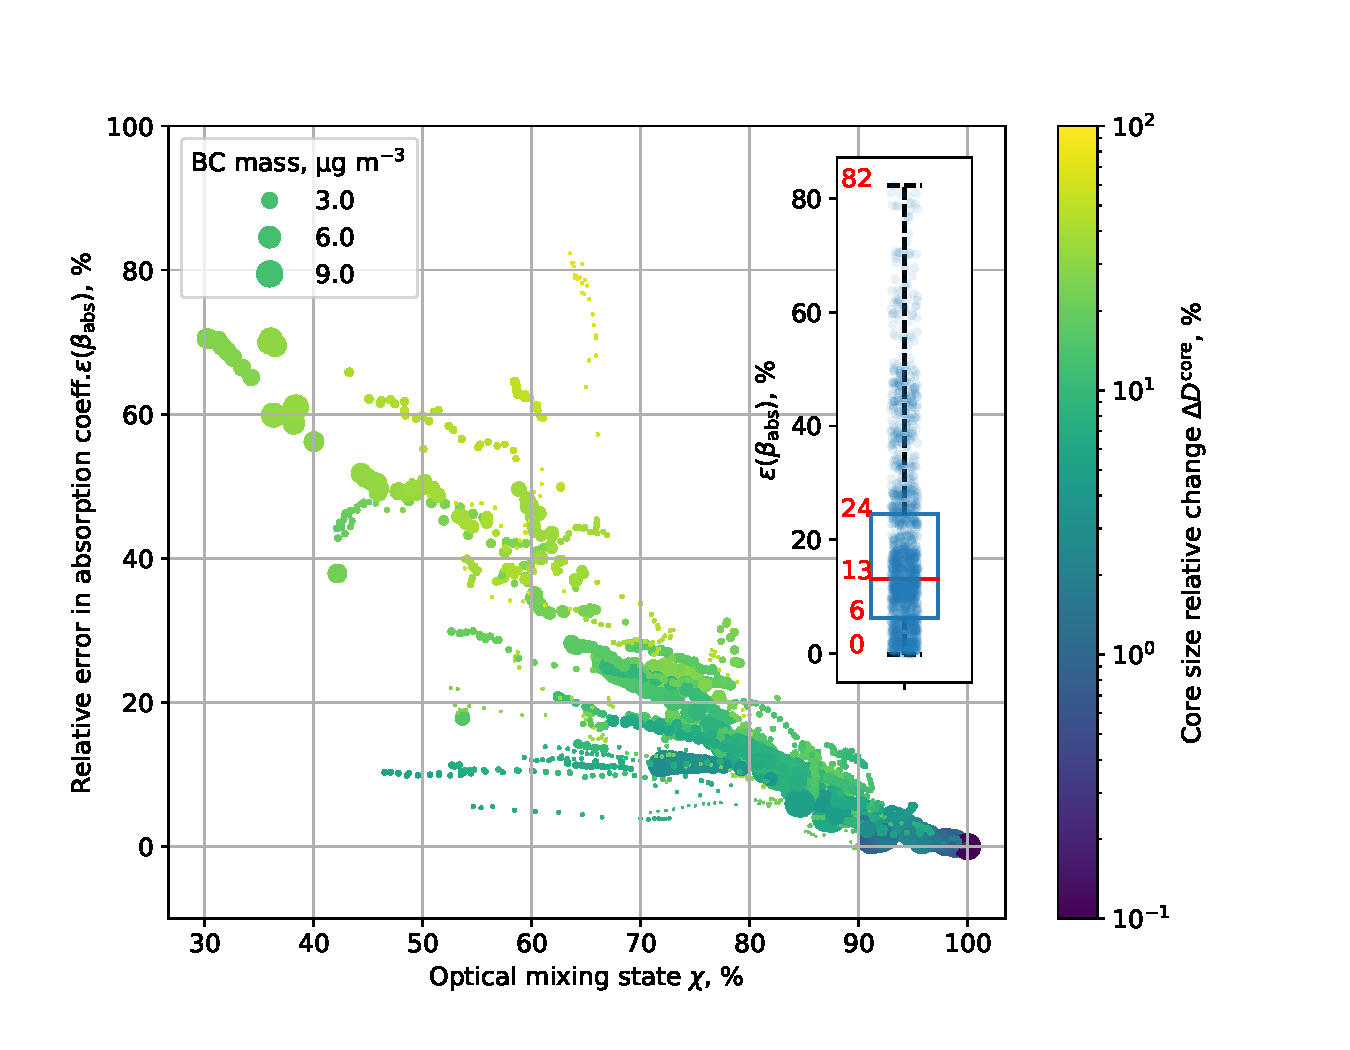
\includegraphics[scale=0.55]{chap4_figs/fig4.pdf}
	\caption{Relative error in absorption coefficients
          $\epsilon(\beta_{\rm abs})$ after composition
          averaging. Each dot represents an aerosol population. The
          color denotes the change of BC diameter due to
          composition-averaging, and the marker size represents BC
          bulk mass in the population. The box plot inset shows the
          distribution of the error. The red line shows the median,
          and the edges of the dashed lines are the minimum and
          maximum values. Red numbers are for the minimum, first
          quartile, mean, third quartile and maximum values.}
	\label{fig3:abs-error}
\end{figure}

For some particles, composition-averaging increases the sizes of BC
cores (while at the same time decreasing the coating thickness) and
for other particles it decreases the BC cores sizes (while increasing
the coating thickness). It is therefore not immediately clear that
composition-averaging consistently causes overestimation of aerosol
absorption coefficients. At per-particle scale, for particles of the
same diameter, $\sigma_{\rm abs}$ increases with increasing BC core,
even though the coating thickness (and hence the absorption
enhancement) decreases (Fig.~\ref{fig_sup1}).

\begin{figure}[H]
	\centering
	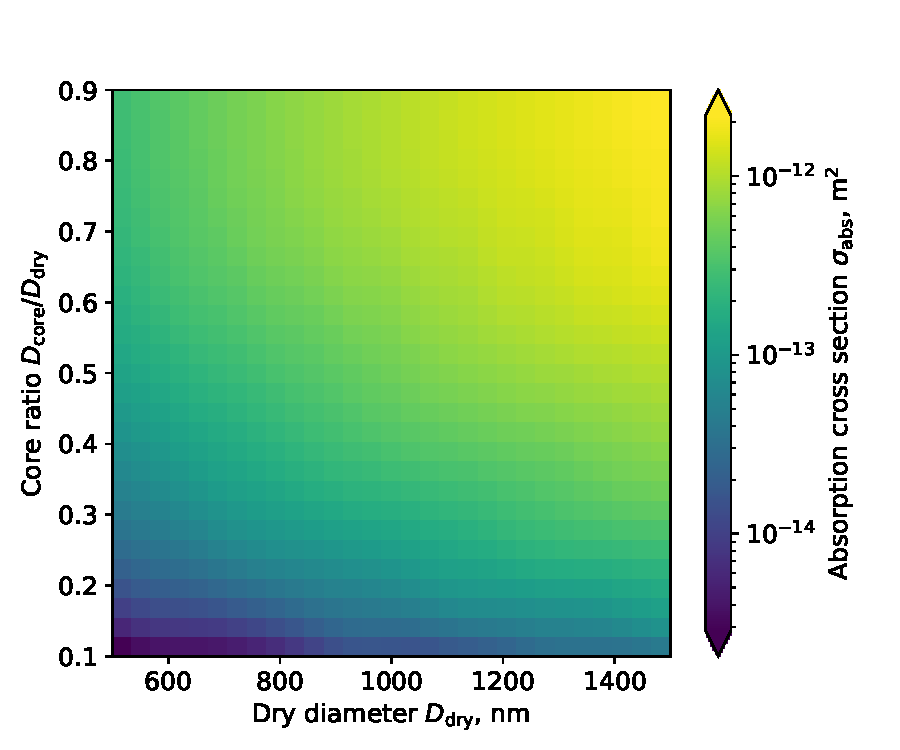
\includegraphics[scale=0.6]{chap4_figs/fig_sup1.pdf}
	\caption{Particle absorption cross section $\sigma_{\rm abs}$ as a function of dry diameter and core ratio}
	\label{fig_sup1}
\end{figure}

%It is important to remember that we preserve the particle size when
%applying composition-averaging. In order to obtain the same species
%mass fraction for particles in the same size bin, particles either
%gain BC and lose coating, or gain coating and lose BC. The change of
%absorption cross section is then the outcome of the balancing effects
%between changes in core size and coating thickness, the latter implies
%changes to the absorption enhancement. To explore the magnitude of
%these two factors, we show the value of absorption cross section
%$\sigma_{\rm abs}$ for one particle as a function of total diameter
%and core ratio, $D_{\rm BC}/D_{\rm dry}$, in
%Fig.~\ref{fig5:abs-exp}a. For particles of a given total diameter,
%$\sigma_{\rm abs}$ increases with increasing BC core size, even though
%the coating thickness (and hence the absorption enhancement)
%decreases.

\begin{figure}
	\centering
	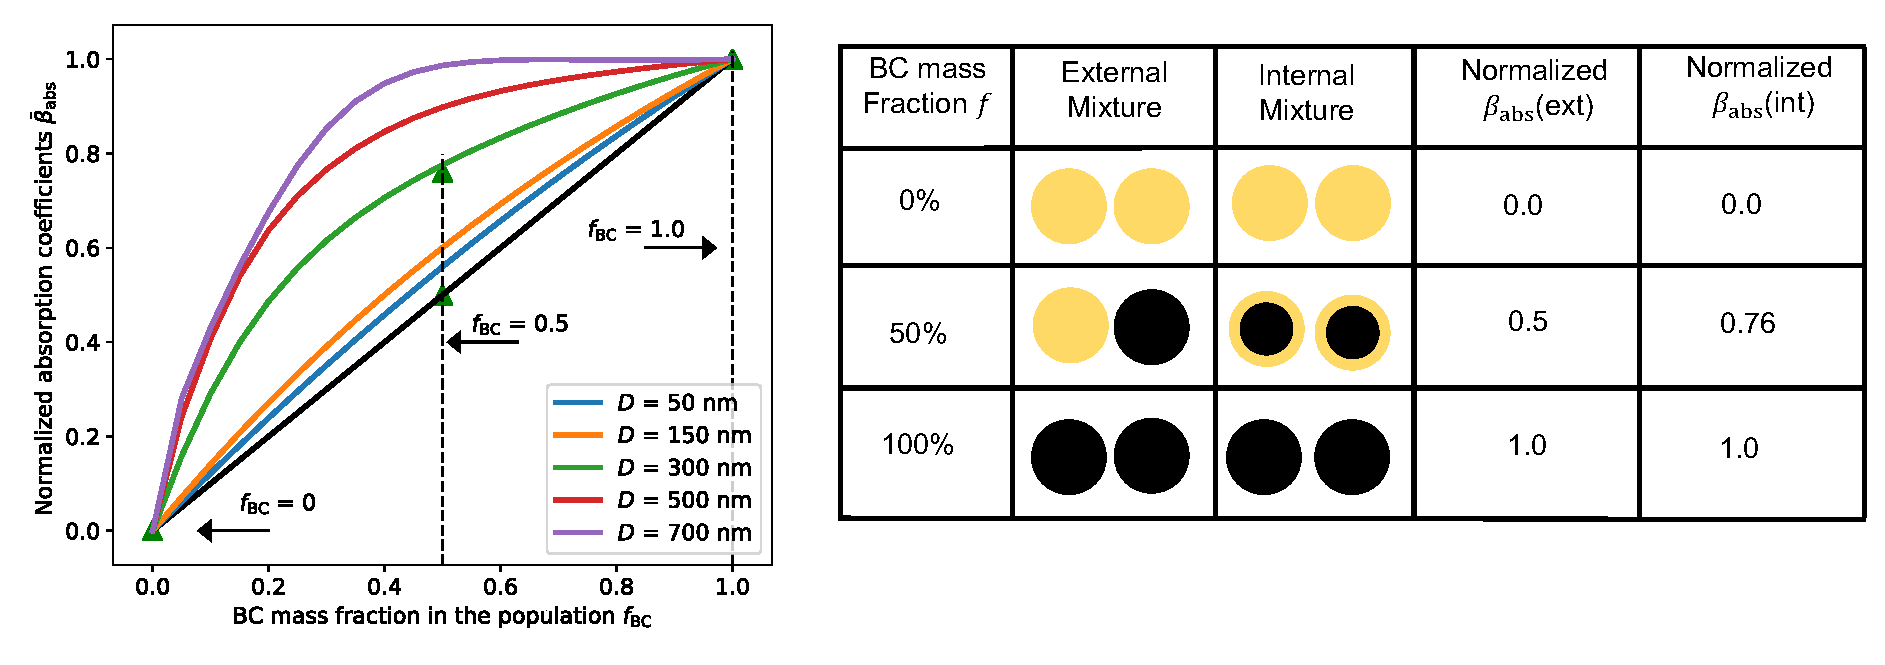
\includegraphics[scale=0.5]{chap4_figs/fig5.pdf}
	\caption{Normalized absorption coefficient as a function of BC
          mass fraction for five monodisperse populations with
          different sizes. The coating species is ammonium bisulfate
          with refractive index 1.47. Absorption coefficients are
          normalized by $\beta_{\rm abs}$ of the population with
          $f_{\rm BC} = 1$ (pure BC). The black line is for BC in
          external mixture. Colored lines are for BC in internal
          mixture of different sizes. Table on the right sketches
          three 300~\unit{nm} internal and external populations with
          BC mass fraction of 0\%, 50\%, and 100\%. Black is for BC
          and yellow for coating species.}
	\label{fig5:abs-exp}
\end{figure}

%However, $\epsilon(\beta_{\rm abs})$ is determined by the entire
%population.
%The internal mixture in each size bin is reached by
%moving species from a group of particles to another group of
%particles.  As the BC mass fraction distribution plots in
%Fig.\ref{fig1:scen} shows, there are two major groups of particles in
%the population: Group 1 are particles with higher BC mass fraction,
%and group 2 are particles with lower BC mass. Particles in group 1
%experience decreased absorbing ability because they are losing BC, and
%it's opposite for particles in Group 2.
%It happened simultaneously in
%each size bin and the net effects are explored in

However, $\epsilon(\beta_{\rm abs})$ is determined by the entire
population. The internal mixture in each size bin is reached by
moving species from a group of particles to another group of
particles.  As the BC mass fraction distribution  in
Fig.\ref{fig1:scen} shows, there are two major groups of particles in
the population: Group 1 are particles with higher BC mass fraction,
and group 2 are particles with lower BC mass. Particles in group 1
experience decreased absorbing ability because they are losing BC, and
vice versa for particles in Group 2.

To further illustrate the effects at the population level, we show the
effects of composition-averaging on the volume absorption coefficient
for a simplified case of five monodisperse populations of different
sizes, starting out with completely externally mixed populations
consisting of BC and ammonium bisulfate
(Fig.\ref{fig5:abs-exp}). Absorption coefficients are normalized by
the absorption coefficient for $f_{\rm BC} = 1$ (pure BC). The black
line shows the normalized volume absorption coefficient for
populations when all particles are externally mixed for bulk BC mass
fractions $f_{\rm BC}$ varying between 0 and 100\%. For external
mixtures, absorption increases linearly with increasing BC mass
fraction (black line). The linear relationship applies for all five
externally-mixed populations with different diameters, so we can only
see one black line in the figure.

The colored lines represent the internally-mixed monodisperse
populations (i.e., after composition-averaging) for different
diameters. These populations all have higher absorption coefficients
compared to the corresponding externally mixed populations. The effect
is more pronounced for larger particles and intermediate BC mass
fractions because the maximum $\Delta_{\rm core}$ is reached. As the
table (Fig.\ref{fig5:abs-exp}) shows, for a 300~\unit{nm} population,
the normalized absorption is 0.76 when the particles are internally
mixed, higher than an external mixed population (0.5). Although this
example is an idealized case since our populations lie between
external and internal mixtures before composition-averaging and are
polydisperse, this illustrates that assuming internal mixture will
lead to absorption overestimation.

The current analysis was based on particles of the same sizes. However,
even in the same size bins, diameters can vary up to several hundred
nanometers. Cases with BC redistribution between particles of
different sizes were further explored in Fig.~\ref{fig_sup2} and
confirmed that the internal mixture assumption will still lead to
positive biases.

Figure~\ref{fig_sup2} shows the relative error when moving BC
from smaller particles to larger particles. Before composition
averaging, small particles $P_1$ have diameter $D_1$, BC fraction
$f_1$ and absorption cross section $\sigma_1$. The large particles
$P_2$ have diameter $D_2$, BC fraction $f_2$ and absorption cross
section $\sigma_2$. After composition-averaging, all particles have BC
mass fraction $f$, with $f_1$ > $f$ and $f_2$ < $f$. Since the overall
BC mass is conserved, we need to move BC mass from $N$ particles of
type $P1$ and $N$ is given by:
\begin{equation}
N = \frac{D_2^3(f-f_2)}{D_1^3(f_1-f)}.
\end{equation}
%\textcolor{red} {This is a bit confusing, because in reality, N is
%given by whatever there is in the bin? And then f is the parameter
%that is calculated as a free parameter?}

The resulting relative change in absorption coefficient for a
population with $N$ particles $P_1$ and one particle $P_2$ is defined
as:
  \begin{equation}{\label{eq7:abs_err}}
   \epsilon(\beta_{\rm abs}) = \frac{(\sigma_2' + N\sigma_1') - (\sigma_2 + N\sigma_1)}{(\sigma_2 + N\sigma_1)},
  \end{equation}
  where $\sigma_2'$, $\sigma_1'$ are the absorption cross section of
  $P_1$ and $P_2$ after composition-averaging, respectively.  As we
  can see from Equation~\ref{eq7:abs_err}, absorption relative error
  $\beta_{\rm abs}$ is determined by the parameters of the two
  particles, including $f_1, f_2, f, D_1, D_2,\sigma_1, \sigma_2$. The
  relations between $\Delta \beta$ and these parameters should be
  nonlinear and it is hard to get a unified trend for different size
  bins.
  
  For an initial trial, figure~\ref{fig_sup2} shows the relative
  error $\beta_{\rm abs}$ when moving BC from particles $P_1$ with
  $D_1 = 600$~\unit{nm} and $f_1$ ranging from 0.4--0.9 to a large
  particle $P_2$ with $D_2 = 1200$~\unit{nm} and $f_2$ ranging from
  0.01--0.15, to make them with unified $f$ at 0.2.  These two
  diameters are the lower and upper boundaries of Bin 5. For the
  ranges considered here, the error is mainly positive, especially for
  $P_2$ with large $f_2$ and $P_1$ with small $f_1$, and $\Delta
  \beta$ reaches 59\% when $f_1$ = 0.4 and $f_2$ = 0.15. These are the
  populations where the increasing absorption ability from the large
  particles overweighting the weakening absorption of those smaller
  particles after redistribution of the species. There are also some
  populations with small overestimation, or even underestimation when
  $P_2$ is with lower $f_2$ and $P_1$ with higher $f_1$. When $f_1$ is
  0.9 and $f_2$ is 0.01, $\Delta \beta$ is $-1.3$\%. These results
  confirm the nonlinear variations when redistributing the species in
  an aerosol population. It is worth to mention that the case in the
  figure is with the simple assumption that particles in the
  population are only with two diameters, but in the simulation cases,
  aerosol populations are more complex with different sizes and BC
  mass fractions in the same size bin.
  
\begin{figure}
	\centering
	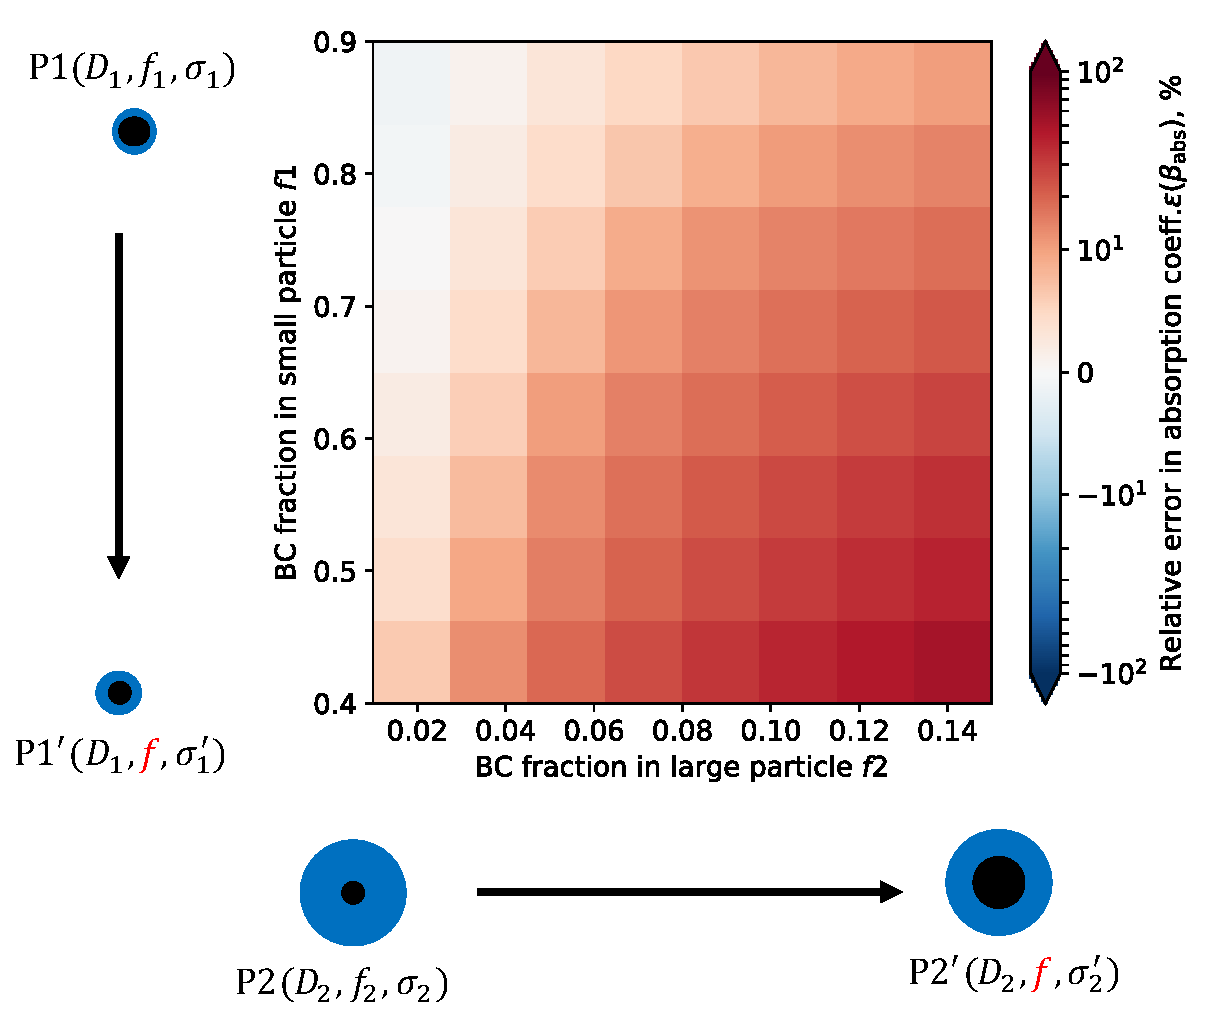
\includegraphics[scale=0.6]{chap4_figs/fig_sup2.pdf}
	\caption{Explanation for particle optical property changes
          after redistribution of BC mass among a
          population with $P1$ and $P2$. $P1$ and $P2$ are two
          particles in the same size bin, but with different diameter
          $D_1$ and $D_2$. $f_1$ and $f_2$ are for the BC mass
          fraction before composition-averaging, and $f$ is the
          unified BC mass fraction after internal mixture assumption
          is used. $\sigma_1$ and $\sigma_2$ are for the absorption
          cross section of the two particles.  $D_1$ = 600~\unit{nm}, $D_2$ =
          1200~\unit{nm} and $f$= 0.2 are the specified values for this
          figure. }
	\label{fig_sup2}
\end{figure}

%The process of composition-averaging is more complicated since the
%particles within a bin are not monodisperse. BC mass is commonly
%transferred from small particles to large particles within the same
%bin, as we can see from the $\Delta{D^{\rm core}}$ being positive in
%Fig.\ref{fig3:abs-error}.
  
%The cases are preliminary explored (see more
%details in Fig.\ref{figsup:abs-exp}), and we found it also produce
%positive bias in absorbing ability when moving BC from several small
%particles with $D$ = 400~\unit{nm} to one large particles with $D$ =
%1200~\unit{nm}.
%At $D$ = 500~nm,
%$\sigma_{\rm abs}$ increases from 2.87$\times10^{-15}$ to
%4.63$\times10^{-14}$ $\rm m^{-2}$ when the core ratio increases from
%0.1 to 0.9.

%Therefore, in the same size bin, composition-averaging moves
%BC from small particles to larger particles to reach the same
%(average) BC fraction. This means that particles in the same size bin
%experience two competing effects: Decreased BC core size in smaller
%particles and increased BC core size in larger particles. The overall
%absorptivity for particles in the same size bin is then determined by
%the net effects of changes in these two group of particles, and the
%effects are explored in
%figure~\ref{fig5:abs-exp}(b). 

%Above all, for the absorption changes, whether BC redistribution
%between particles with same size or different size, absorbing ability
%of an aerosol population is more likely to be overestimated when
%moving from external to internal mixture. With composition-averaging,
%the same amount of BC are distributed to more particles and increases
%absorption ability. This redistribution of BC is universal when
%applying internal mixture assumptions, and it explains why absorption
%are overwhelming overestimated in the populations after composition
%averaging. The effects of redistribution can be significant for
%populations that are more externally mixed, or contain less fraction
%of BC where small changes can lead to large biases. It should be
%careful when using internal mixture assumptions for these populations.

\subsection{Error in aerosol scattering due to composition-averaging}
Considering the volume scattering coefficient, composition-averaging
resulted in a negative relative error
(Fig.\ref{fig6:scat-err}). Similar to what we found for
$\epsilon(\beta_{\rm abs}$), the magnitudes of $\epsilon(\beta_{\rm
  scat})$ decreased with increasing $\chi$, but were overall smaller,
with the largest underestimation of $-$32\% for a population with
$\chi$ = 40\% and a median of $-$1.2\%.

\begin{figure}
	\centering
	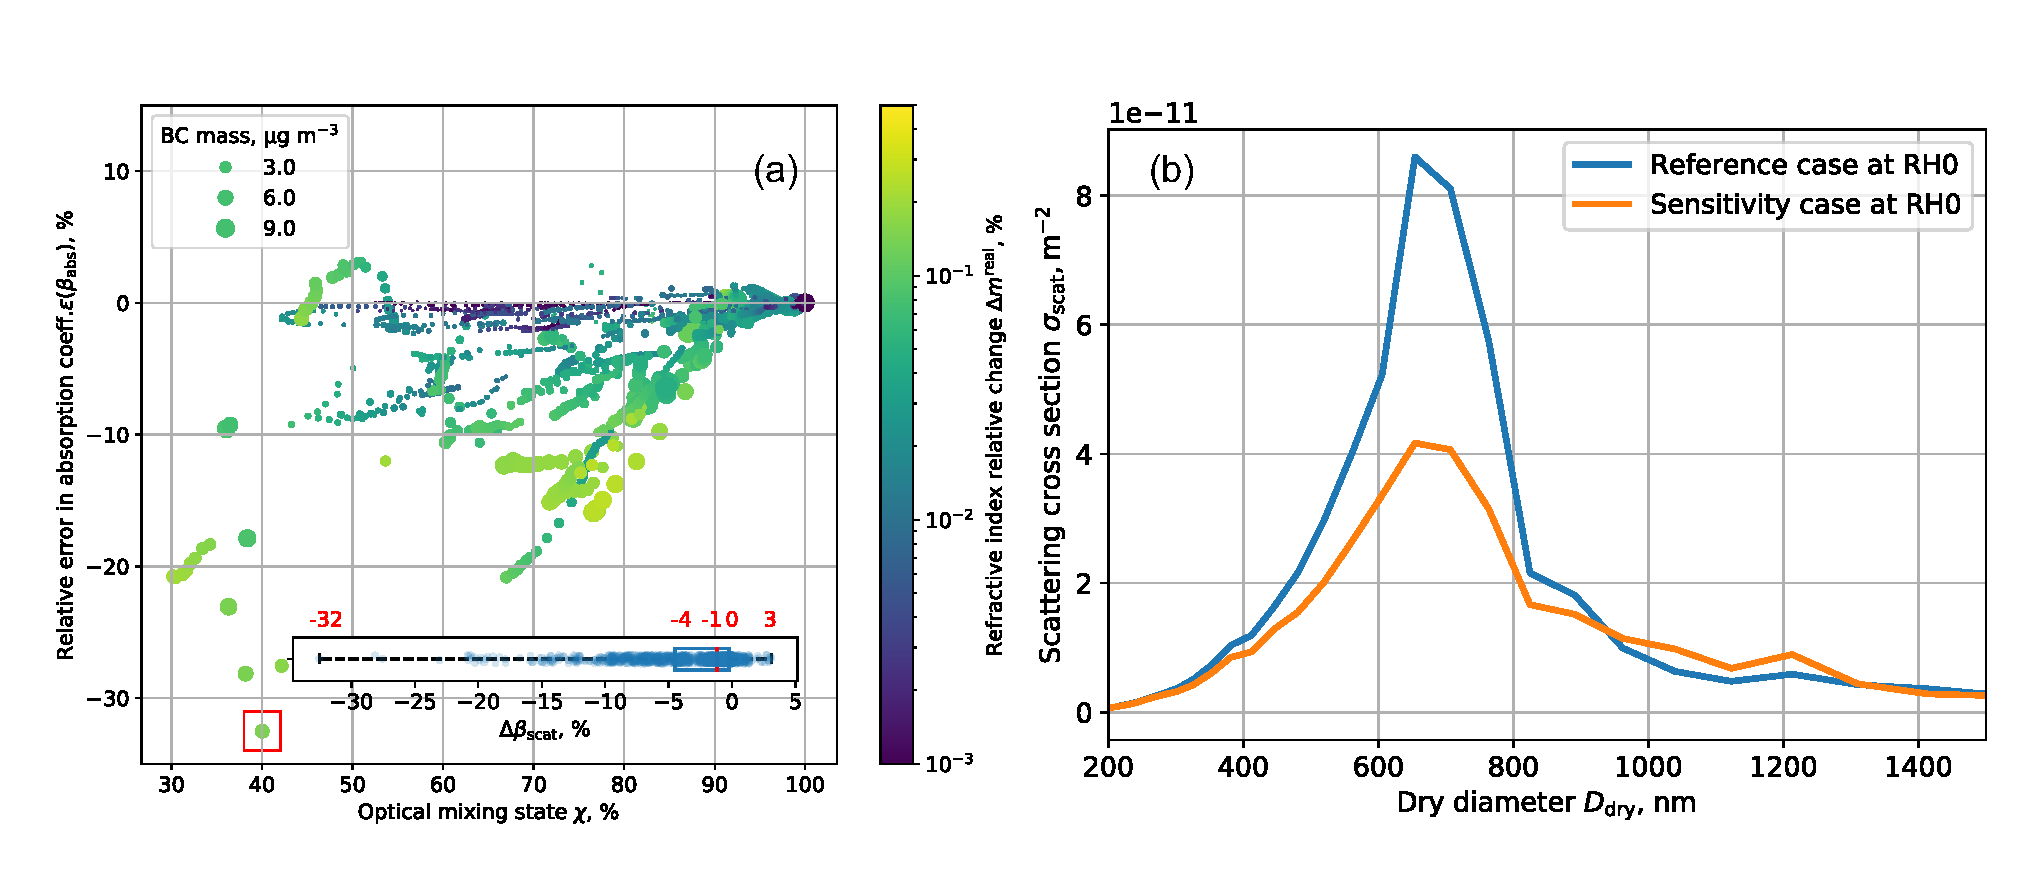
\includegraphics[scale=0.50]{chap4_figs/fig6.pdf}
	\caption{(a) Same as Figure~\ref{fig3:abs-error}, but for
          $\epsilon({\beta_{\rm scat}})$. The color is for
          refractive index relative change and the marker size represents BC bulk
          mass in the population. Red box is the populations analyzed in (b). 
          (b) Size-resolved scattering coefficients at
          reference and sensitivity scenario library.  This population
          is from scenario 77 at 2h.}
	\label{fig6:scat-err}
\end{figure}

There are two factors that can affect particle scattering ability
after composition-averaging, the change of the BC core size (and the
corresponding change in coating thickness), and the change in the
refractive index of the coating. As Fig.~\ref{fig8:scat-exp} shows,
adding a BC core decreases the scattering ability for particles with
diameters less than 1200~\unit{nm}, which are the typical size ranges
considered in our study. This explains the larger scattering
underestimation with higher BC mass concentration in
Fig.~\ref{fig6:scat-err}.

\begin{figure}
	\centering
	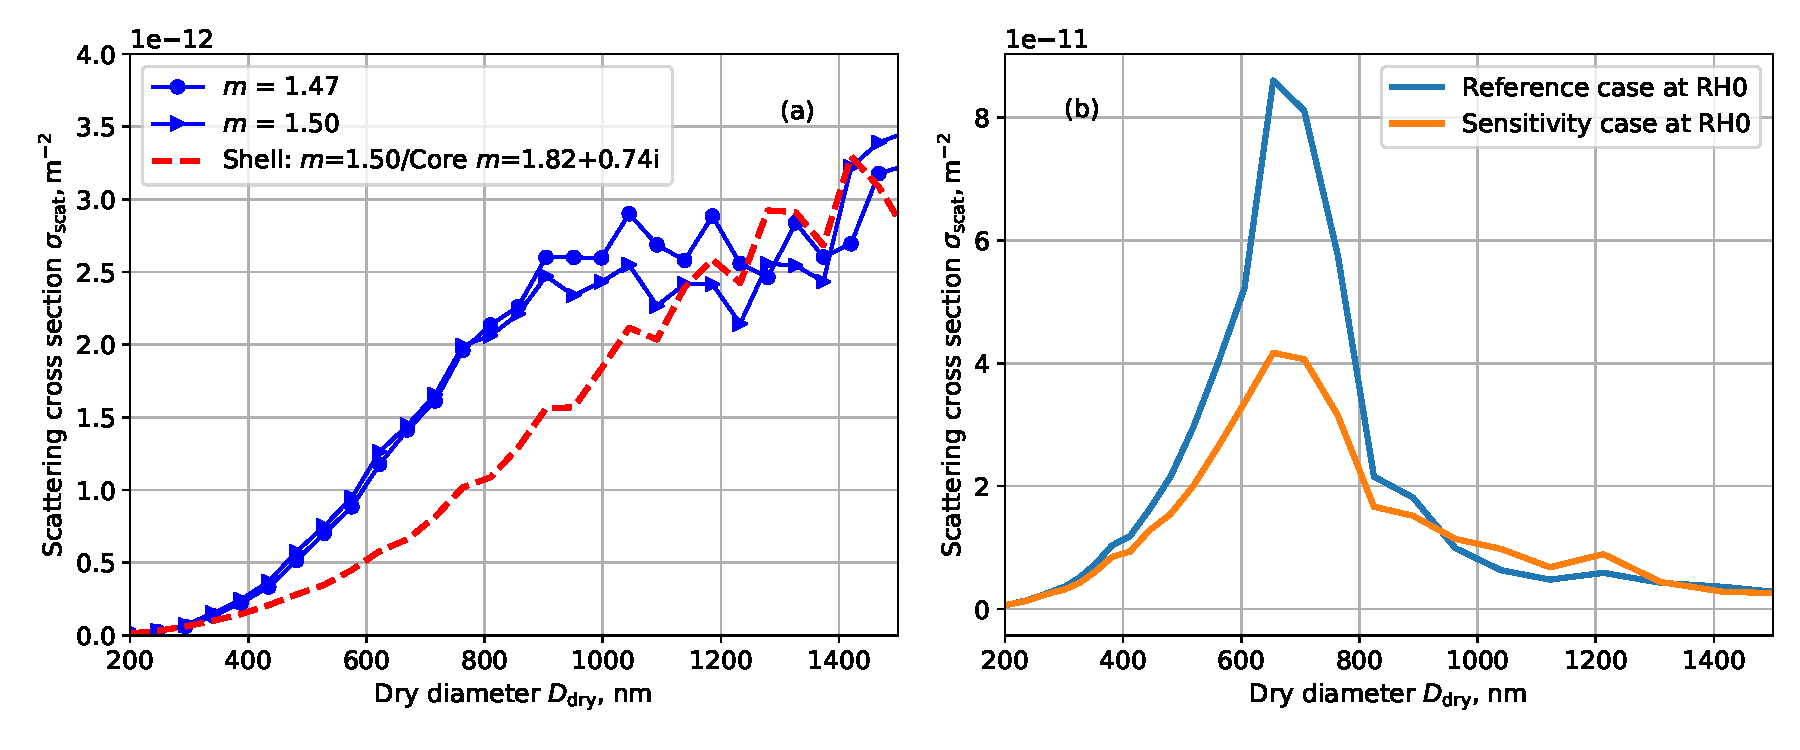
\includegraphics[scale=0.50]{chap4_figs/fig7.pdf}
	\caption{Relation between scattering ability, refractive
          indices and diameter. Blue lines are for non-absorbing
          particles and symbols indicate different refractive
          index. Red line is for absorbing particles including a BC
          core of $0.2D$.}
	\label{fig8:scat-exp}
\end{figure}

To further explore the effects of coating volume changes,
Fig.~\ref{fig6:scat-err}(b) shows the size-resolved scattering
coefficients before and after composition-averaging for the aerosol
populations from scenario 77 at 2h, which produced the largest
scattering coefficients underestimation ($-$32\%). There is a
significant decrease of $\sigma_{\rm scat}$ in the size range of
400--800~\unit{nm} in the sensitivity populations, and the core ratio
increment in bin 4 is responsible for this decrease
(Fig.~\ref{fig_sup3}).

\begin{figure}[H]
	\centering
	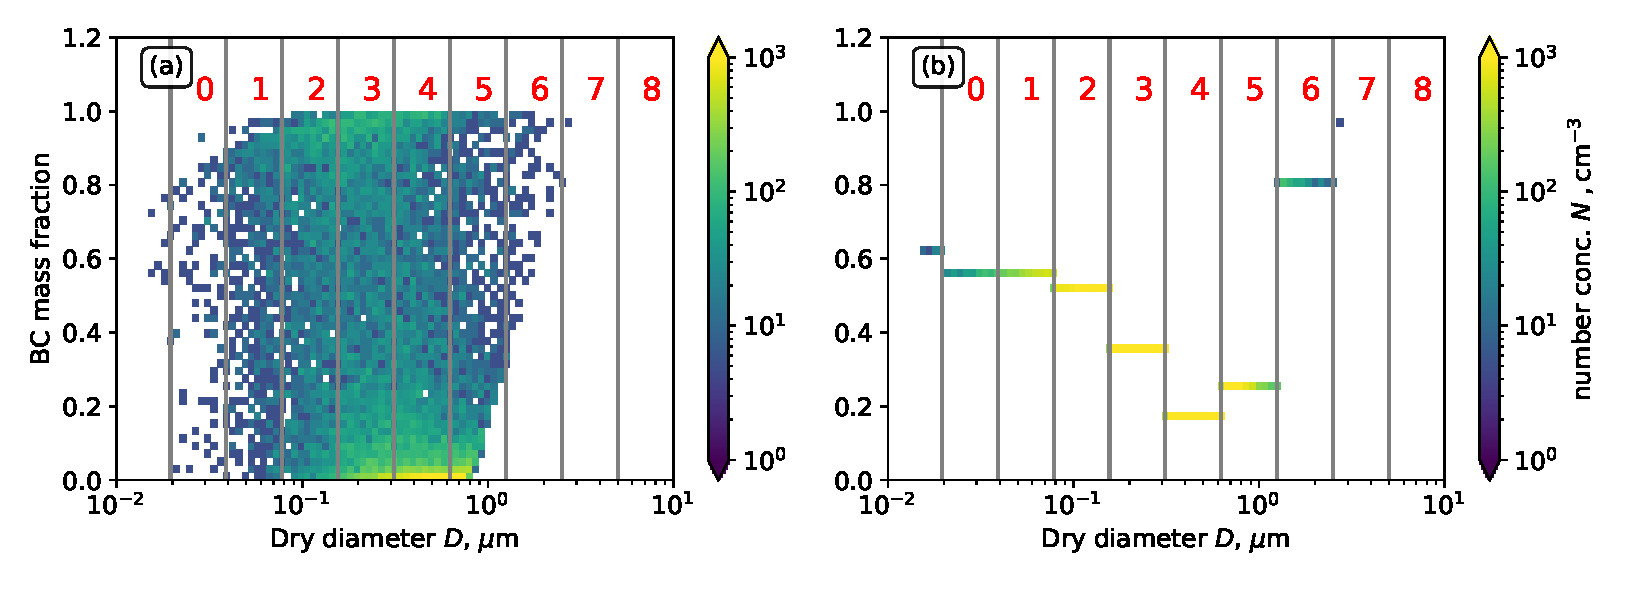
\includegraphics[scale=0.50]{chap4_figs/fig_sup3.pdf}
	\caption{Two-dimensional distributions of BC mass fraction in (a) Reference scenario and (b) Sensitivity scenario at RH0. 
	 This population is from scenario 77 at 2h.}
	\label{fig_sup3}
\end{figure}

The blue lines in Fig.~\ref{fig8:scat-exp} show the scattering cross
sections for two different real refractive indices. For particles with
diameters between 800 and 1200~\unit{nm}, a lower refractive index
leads to a larger scattering cross section, even though the difference
is smaller than the change caused by adding a BC core. Similar to the
BC core size change $\Delta D^{\rm core}$ {in
  Figure~\ref{fig3:abs-error}}, we defined a volume-weighted
refractive index change, $\Delta{m^{\rm real}}$, to help understand
the changes in scattering. The index change is defined as:
\begin{equation}
    \displaystyle \Delta{m^{\rm real}}=\frac{\sum_{i=1}^{N} V_i {m^{\rm real}}' - \sum_{i=1}^{N} V_i {m^{\rm real}}}{\sum_{i=1}^{N} V_i {m^{\rm real}}},
\end{equation}
where $i$ is the particle index, $V_i$ is the particle volume,
${m^{\rm real}}$ is the real part of the coating refractive index of
the particles in the reference library, and ${m^{\rm real}}'$ is for
particles in the sensitivity library. As shown in
Fig.~\ref{fig6:scat-err}, aerosol populations with small errors in
scattering tend to be associated with small $\Delta{m^{\rm
    real}}$. For more externally-mixed populations (with lower
$\chi$), $\Delta{m^{\rm real}}$ tended to be larger.

For the effects of composition-averaging for particle scattering, we
conclude that at a given value of $\chi$, the magnitude of
$\epsilon(\beta_{\rm scat})$ was determined by the change in
core/coating volumes and by changes in the coating refractive
index. The inccrease of BC core sizes after composition-averaging is
the major factor for the decrease of the scattering
coefficients. Populations with large underestimation are those with
higher BC mass concentrations and large refractive index changes.

\section{The effects of water uptake on aerosol optical properties}
\label{sec:wet-case}
The analysis so far was based on dry aerosol populations. In this
section we investigate the impact of water uptake on the errors in
absorption and scattering by considering RH values of 50\% and 90\%.
As a reminder, we performed composition-averaging on the dry
population first, and then calculated water uptake based on the
averaged composition for 50\% RH and 90\% RH, respectively.

Considering all populations, the range of relative errors in
$\beta_{\rm scat}$ decreases with increasing RH. The median value of
$\epsilon(\beta_{\rm scat})$ decreased from 1.2\% for dry populations
RH0 to 0.2\% for 90\% RH, and the IQR decreased from 4.2\% to 1.5\%
(Fig.\ref{fig9:RH90-RH10-opt-scat}a).  In contrast, the range of
relative errors in $\beta_{\rm abs}$ remains approximately the same
(Fig.\ref{fig9:RH90-RH10-opt-scat})b. The median value of error
$\epsilon(\beta_{\rm abs})$ remained at 13\% and IQR decreased from
18.3\% to 14.9\%.
\begin{figure}
	\centering
	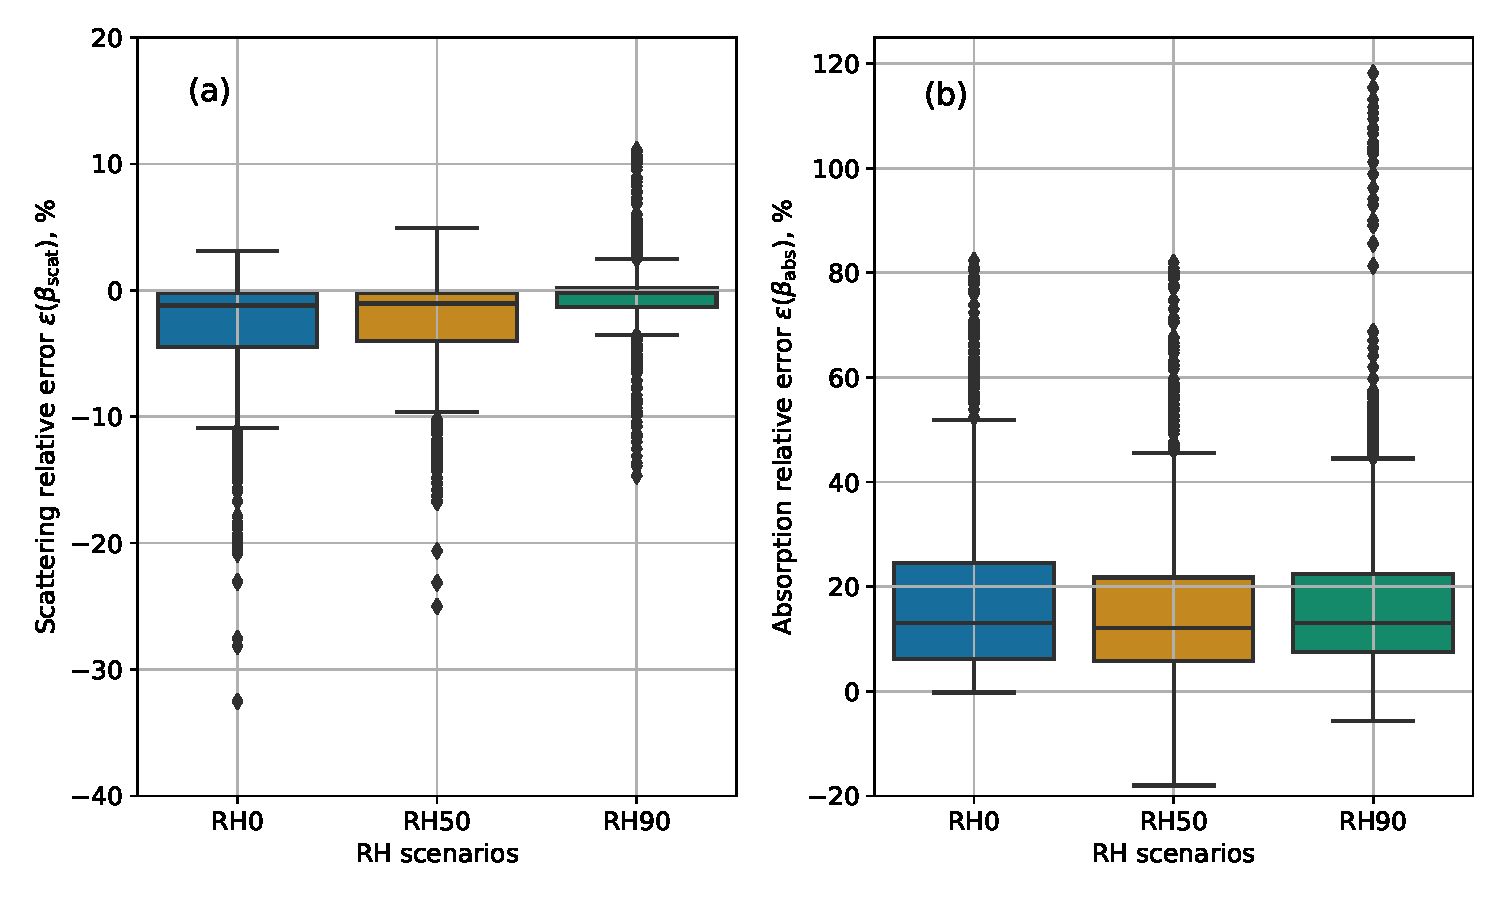
\includegraphics[scale=0.5]{chap4_figs/fig8.pdf}
	\caption{Box plot of (a) scattering relative error
          $\epsilon(\beta_{\rm scat})$ and (b) absorption relative
          error $\epsilon(\beta_{\rm abs})$ at three RH levels (0\%,
          50\% and 90\%). Dots are the populations with values outside
          Q3 + 1.5IQR. }
	\label{fig9:RH90-RH10-opt-scat}
\end{figure}

%The relationship between the errors for dry conditions and for 90\% RH
%is further explored in Fig.\ref{fig10:RH90-RH10-opt-scat}.  Scattering
%error $\epsilon(\beta_{\rm scat})$ is above the 1:1 line, indicating
%for the same population, the magnitude of the error introduced by
%composition-averaging decreased when water uptake is considered. The
%larger the water uptake (indicated by color), the closer the error is
%0\%, and this applies to populations with both low and high scattering
%coefficients (indicated by marker size). The effect of water uptake on
%$\epsilon(\beta_{\rm abs})$ is small, with most populations falling
%close on the 1:1 line. Outliers are populations with very less BC and
%absorbing ability can change a lot even with a small change of the
%values. This is similar to what we found in the dry population, where
%minor distribution of chemical species will resulted in higher error
%when the particles contain less BC.

\begin{figure}
	\centering
	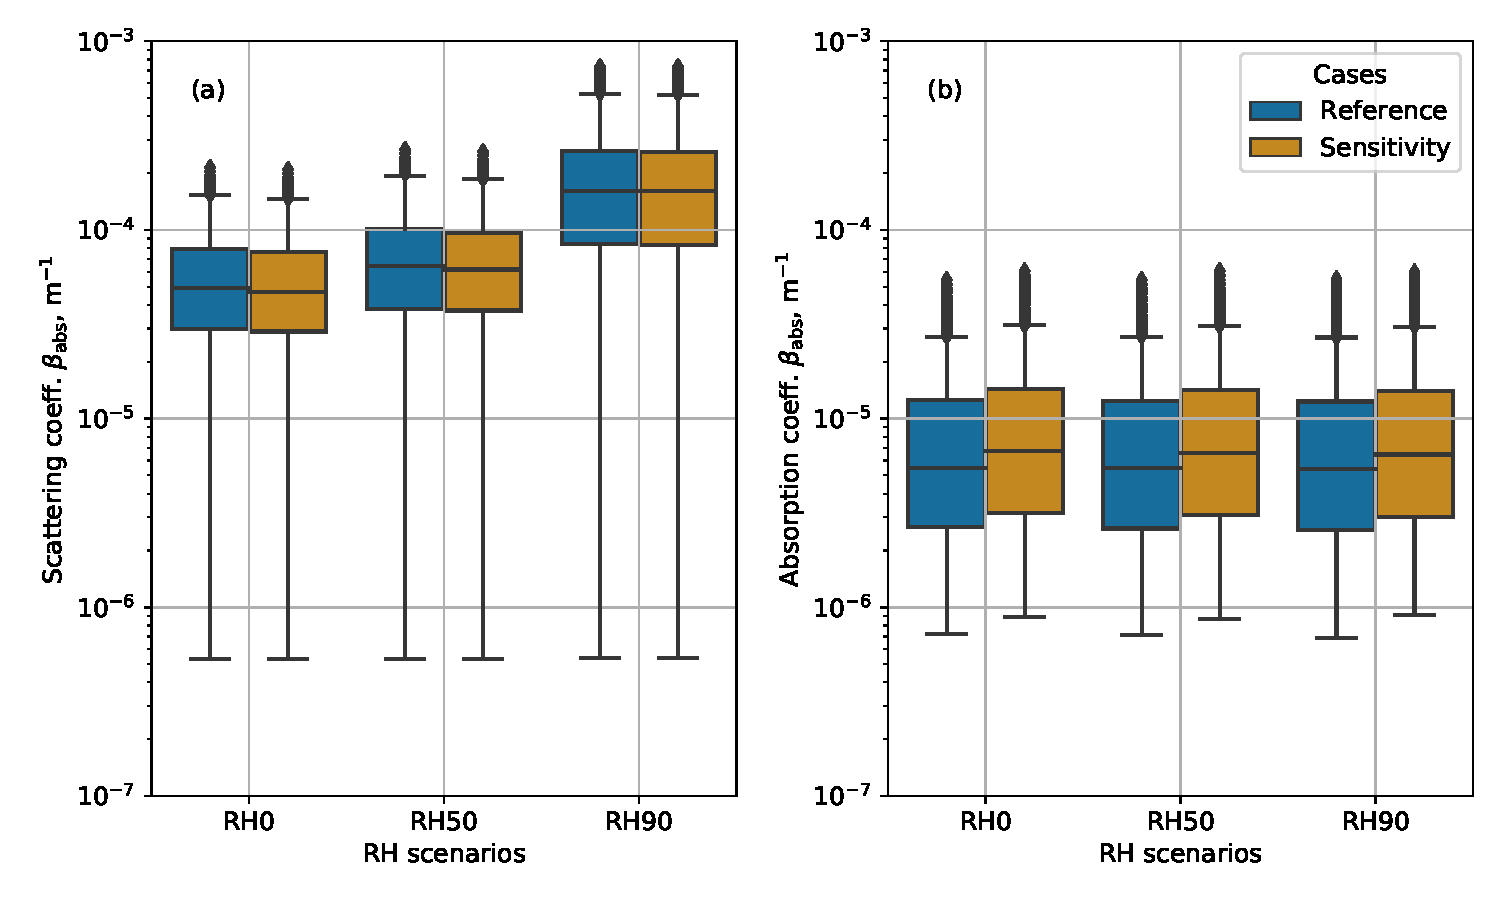
\includegraphics[scale=0.50]{chap4_figs/fig9.pdf}
	\caption{Box plots of (a) volume scattering coefficients
          $\beta_{\rm scat}$, (b) volume absorption coefficients
          $\beta_{\rm abs}$ at the RH levels of 0, 50, 90\%. Dark blue
          is for populations in reference scenario and Dark orange is
          for sensitivity scenario.}
	\label{fig10:RH90-RH10-opt-scat}
\end{figure}
  
The different response of $\epsilon(\beta_{\rm \rm abs})$ and
$\epsilon(\beta_{\rm \rm scat})$ after the population become
humidified is due to changes of the coating species after water
uptake, and this is examined in Fig.~\ref{fig10:RH90-RH10-opt-scat}.
At humidified environment, scattering coefficients increased
significantly.  Compared with median $\beta_{\rm scat}$ = 4.42$\times$
$10^{-5}$~\unit{m^{-1}}at RH = 10~\%, $\beta_{\rm scat}$ increased to
5.90$\times$ $10^{-5}$ ~\unit{m^{-1}} and 14.8$\times$ $10^{-5}$
~\unit{m^{-1}} at RH = 50~\% and at RH = 90~\%, respectively.  The
enhancement ratio, defined by the $\beta_{\rm scat}$ values in higher
RH cases and dry case, are 1.33 at RH = 50\% and 3.35 at RH = 90\% in
our scenario populations, which are in accordance with the previous
studies \citep{Titos2016, Burgos2020}. However, the differences
between the reference and sensitivity are small and keep almost
unchanged at higher RH environment, which implies the water absorption
ability is not affected by species redistribution.  The increase of
scattering coefficients and insignificant change of the differences
explain the decrease of $\epsilon(\beta_{\rm \rm abs})$ with
increasing RH. As for absorption coefficients in humidified
environment, the differences between reference and sensitivity cases
stay the same and the effect of RH in absorption coefficients is
minimal.

\section{Errors in single scattering albedo and implications for directive radiative forcing}
\label{sec:ssa}
The changes of scattering and absorption coefficients lead to changes
in SSA, which is an important quantity that determines radiative
forcing. With the definition of SSA, we can calculate the absolute
error $\Delta$SSA as:
\begin{equation}{\label{eq8:ssa_err}}
\Delta {\rm SSA} = \frac{\beta_{\rm \rm scat}'}{\beta_{\rm \rm scat}' + \beta_{\rm \rm abs}'} - \frac{\beta_{\rm \rm scat}}{\beta_{\rm \rm scat} + \beta_{\rm \rm abs}} = \frac{\beta_{\rm \rm scat}'\beta_{\rm \rm abs} - \beta_{\rm \rm scat}\beta_{\rm \rm abs}'}{(\beta_{\rm \rm scat}' + \beta_{\rm \rm abs}')(\beta_{\rm \rm scat} + \beta_{\rm \rm abs})},
\end{equation}
where $\beta_{\rm scat}'$, $\beta_{\rm abs}'$ are for the scattering
and absorption coefficients after composition-averaging. Based on the
previous analysis, we know that $\beta_{\rm scat}'$ tends to be lower
than $\beta_{\rm scat}$ and $\beta_{\rm abs}'$ greater than
$\beta_{\rm abs}$. Combining these changes with
equation~\ref{eq8:ssa_err}, these variations will result in negative
values for $\Delta$SSA and the relative error $\epsilon(\rm SSA)$,
which is confirmed by Fig.~\ref{fig12:ssa-err}.


In order to connect $\epsilon(\rm SSA)$ with $\epsilon(\beta_{\rm
  scat})$ and $\epsilon(\beta_{\rm scat})$, we sorted the populations
by $\epsilon(\beta_{\rm scat)}$ and $\epsilon(\beta_{\rm abs)}$ ranges
and calculated the mean $\epsilon(\rm SSA)$ for each
$\epsilon(\beta_{\rm scat})$-$\epsilon(\beta_{\rm abs)}$ bin. For all
three RH levels, $\epsilon(\rm SSA)$ was negative, meaning that
composition-averaging causes an underestimation of SSA. The largest
$\epsilon(\rm SSA)$ ($-22$\% occured for the largest underestimation
in $\epsilon(\beta_{\rm scat})$ in the RH = 0\%
environment. Populations with $\epsilon(\rm SSA)$ lower than $-10$\%
were related to populations with large negative magnitudes of
$\epsilon(\beta_{\rm scat})$. Relative errors in SSA decreased in more
humidified environment, accompanied by decreasing errors in scattering
coefficients. The median $\epsilon(\rm SSA)$ decreased from $-7.5$\%
for RH = 0\% to $-2.2$\% in RH = 90\%.

\begin{figure}
	\centering
	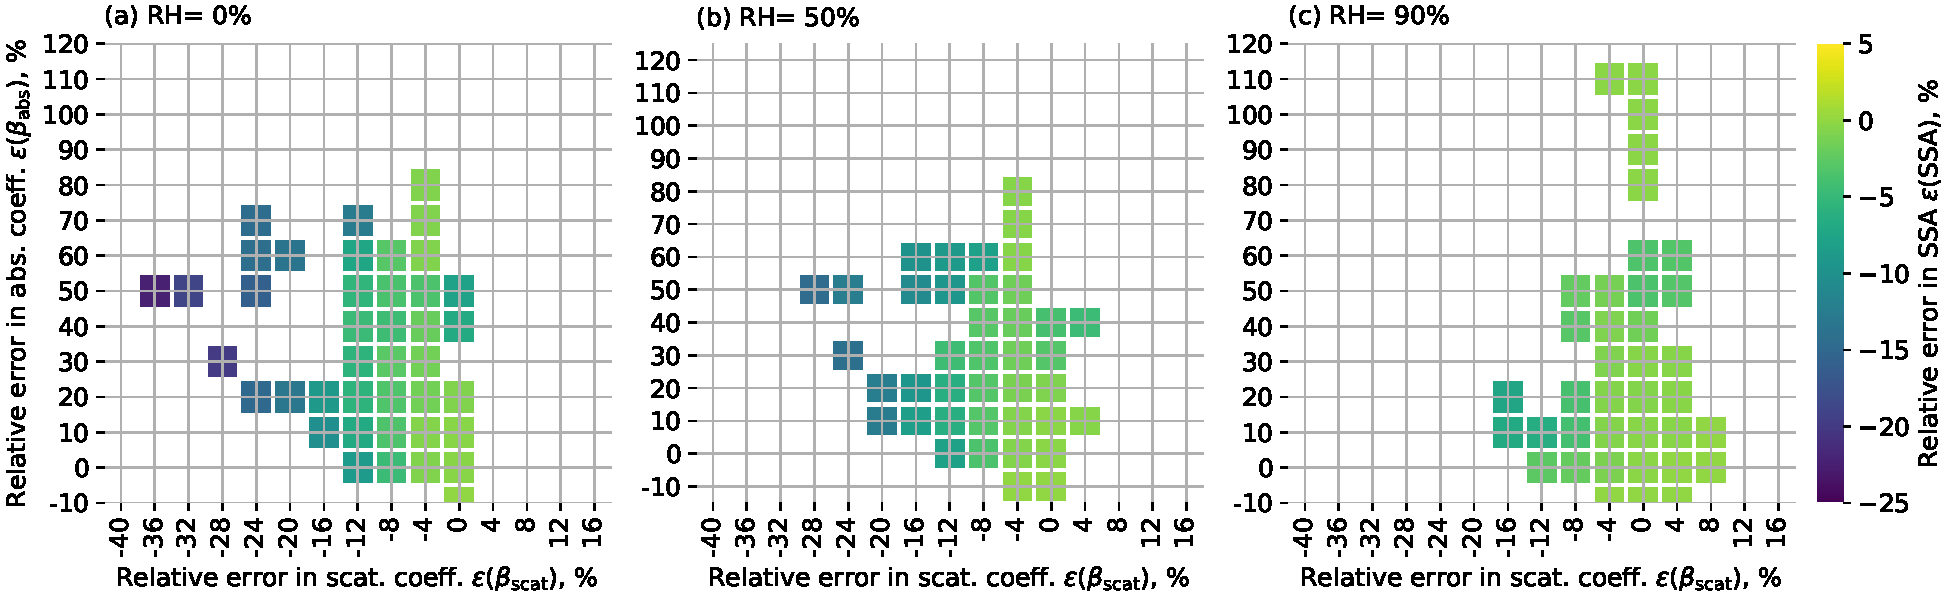
\includegraphics[scale=0.50]{chap4_figs/fig10.pdf}
	\caption{Relation between errors in SSA, scattering and
          absorption coefficients. Color represents the mean
          $\epsilon$(SSA) in the corresponding $\epsilon(\beta_{\rm
            scat})$ and $\epsilon(\beta_{\rm \rm abs})$ histogram.}
	\label{fig12:ssa-err}
\end{figure}

The underestimation of SSA can have significant impacts in calculating
direct radiative forcing. \citet{mccomiskey2008direct} evaluated the
response of directive radiative forcing to changes of several
quantities, including aerosol optical depth, single
scattering albedo and other related factors. They found the total
uncertainties in directive radiative forcing ranged from 0.2 to 3.1
\unit{W\,m^{-2}} and SSA introduced the largest uncertainties. Through
perturbation analysis, \citet{loeb2010direct} also found the SSA to be
the dominant factors for direct radiative forcing uncertainties and
with SSA perturbed $\pm$ 0.06 over ocean and $\pm$ 0.03 over land, the
resulted uncertainties in direct aerosol radiative forcing range
between $-$0.55 and 1.11 \unit{W\,m^{-2}}. Considering the SSA error of
$-$7.5\% and $-$2.2\% in dry and humidified environment in the current
simulation, combining the median SSA values (Fig.~\ref{fig_sup4}), these errors
translate to $-$0.069 and $-$0.021 perturbation level in SSA,
respectively, and lead to the same order of magnitude of direct
radiative forcing uncertainties as \citeauthor{loeb2010direct} found.

\begin{figure}[H]
	\centering
	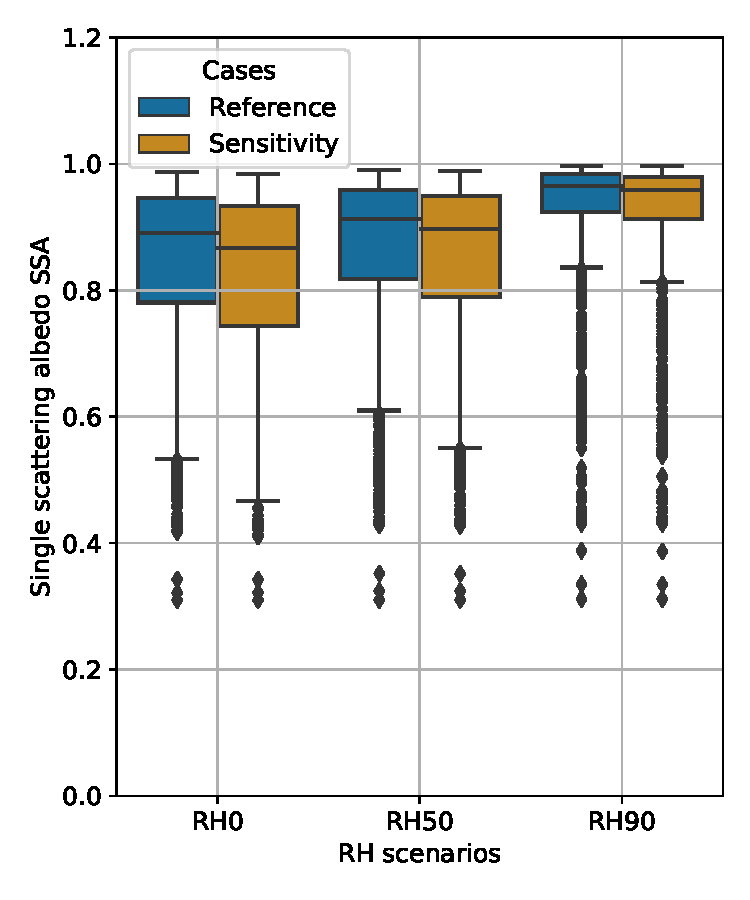
\includegraphics[scale=0.50]{chap4_figs/fig_sup4.pdf}
	\caption{Box plots of single scattering albedo at different RH levels. Dark blue is for populations
	in reference scenario and Dark orange is for sensitivity scenario.}
	\label{fig_sup4}
\end{figure}

\section{Conclusion and discussion}
\label{sec:conclusion}

Simplified representation of aerosol mixing state used in current
regional or global models may introduce errors in simulating aerosol
optical properties, thus leading to uncertainties in calculating
directive radiative forcing. In this study, the errors introduced by
internal mixture assumptions used in sectional aerosol models were
systematically quantified. We created a reference scenario library
with 1800 aerosol populations by performing particle-resolved aerosol model
simulations with PartMC-MOSAIC. We constructed a sensitivity library
where particles were internally mixed in a prescribed set of size bins
by applying composition-averaging. Aerosol populations from the
reference and sensitivity library were then exposed to three different
RH levels to understand the relative role of chemical species and
water redistribution introduced by the internal mixture assumption.

%Errors in dry environment
The internal mixture assumption generally led to an overestimation of
the volume absorption coefficients and an underestimation of the
volume scattering coefficients. The relative errors for
$\epsilon(\beta_{\rm abs})$ and $\epsilon(\beta_{\rm scat})$ reached
up to 70\% and $-$32\%, respectively. The relative errors generally
increased for more externally-mixed populations, although at a given
value for $\chi$ a range of errors can be found, especially for the
error in the scattering coefficient. For the error in the absorption
coefficient, this range can be explained by the magnitude of BC core
size changes that are induced by composition-averaging. For the error
in the scattering coefficient, it can be explained by the magnitude of
the changes in the refractive index of the coating that are induced by
the composition-averaging.

%Errors in wet environment
For the cases with RH of 50\% and 90\%, the bulk aerosol water content
was almost identical for the aerosol populations in reference and
sensitivity libraries. The relative error in the volume absorption
coefficient $\epsilon(\beta_{\rm abs})$ displayed a similar pattern
for RH of 50\% and 90\% compared to the dry environment. The relative
error in the volume scattering coefficient $\epsilon(\beta_{\rm
  scat})$ decreased for higher relative humidities because of the
enhanced scattering ability through hygroscopic growth.

%Errors in SSA and implication for radiative forcing
The absorption overestimation and scattering underestimation resulted
in an underestimation of SSA. Populations with the largest
underestimation of SSA were associated with populations with the
largest underestimation in scattering. At RH = 90\%, decreasing
relative scattering error also leads to smaller SSA inaccuracy. Based
on previous studies in the literatrue these SSA error magnitudes
translate to uncertainty ranges between $-$0.55 and 1.11 \unit{W\,
  m^{-2}} in direct aerosol radiative forcing.
  
%limitation 1: shape
It is worth emphasizing that we used Mie theory with core-shell
configuration to calculate optical properties assuming spherical
particle shapes. Our results are therefore most representative of
BC-containing populations, where the BC core is collapsed rather than
a fractal aggregate \citep{china2013morphology,
  china2015morphology}. More accurate methods, such as discrete dipole
approximation (DDA) should be used to represent these more irregular
particle shapes \citep{scarnato2013effects,
  curtis2008laboratory,luo2019optical, wu2020light}.
%\edits{We also
%  acknowledge that for more bare BC particles, i.e. more
%  externally-mixed BC, the impact of mixing state on optical
%  properties (absorption and scattering) is believed to be limited}.

%limitation 2: refractive indices
The species complex index should be also explored further. For current
work, we used refractive index value 1.82 + 0.74$i$ for BC, which is
close to the medium index suggested by \citet{stier2007aerosol}, but
it can vary among different measurements.  Furthermore, we did not
consider the absorbing abilities of organic carbons, and several
studies had lately been conducted to constrain the imaginary index
values of brown carbon \citep{liu2020lifecycle}. \citet{Esteve2014}
has showed the index of organic aerosols are a large uncertainties in
quantifying aerosol absorbing abilities. At last, for current aerosol
populations, we focused on fine mode particles and ignored sea salt
and dust particles, and it should also be important to include these
particles for reducing the uncertainties in direct radiative forcing.

%%%%%%%%%%%%%%%%%%%%%%%%%%%%%
%%%%%%%%%Chapter 5%%%%%%%%%%%
%%%%%%%%%%%%%%%%%%%%%%%%%%%%%
\chapter{Conclusions}
\label{chap5}
\section{Work summary}
This dissertation improved the understanding of aerosol aging
processes in clouds and the role of aerosol mixing state for aerosol
scattering and absorption of sunlight. The key questions for this work
were: (1) To what extent does aqueous phase chemistry change the
aerosol mixing state of the aerosol that entered the cloud, and what
is the role of coagulation between the interstitial particles and
cloud droplets for mixing state of the aerosol? (2) Given the degree
of the aerosol population mixing state, what are the errors in aerosol
optical properties introduced by the internal mixture assumption and
what are the causes?

In answering the first question, I designed cloud parcel simulations
by using a newly developed particle-resolved aqueous chemistry
model. It is a zero-dimensional adiabatic cloud parcel model with
comprehensive aqueous phase reactions. The model was evaluated by
comparing with results from the literature and was proved to be able
of capturing the aqueous reactions involved in sulfate formation
(Chapter~\ref{chap2}). I quantified aerosol mixing state changes after
aqueous chemistry processes and generalized the findings by using
aerosol populations from different urban environment. I also evaluated
the role of coagulation between interstitial particles and cloud
droplets for aerosol mixing state (Chapter~\ref{chap3}).

For the second question, I developed a framework to quantify the error
in aerosol optical values introduced by simplified aerosol
representation (Chapter~\ref{chap4}). I created an a reference aerosol
population ensemble with a wide variety of aerosol mixing state using
PartMC-MOSAIC. I quantified the errors by comparing the optical
properties from the reference populations to populations where the
composition was averaged. I developed several metrics to explain the
errors. I further explored the impact of water uptake on the optical
value errors by exposing these populations to different levels of
relative humidity.

\section{Contributions}
{\bf Quantifying cloud processing effects on aerosol properties.} With
the newly coupled particle-resolved aqueous chemistry model, I
quantified the changes of aerosol properties after cloud processing on
a per-particle level. For aerosol populations dominated by fresh
emissions, adding secondary species produced from aqueous chemistry
increased the particle diversity. However, whether the overall
population became more or less internally mixed depended on the
relative changes of average particle diversity ($D_{\alpha}$) and bulk
aerosol diversity ($D_{\gamma}$), which determines the aerosol mixing
state metrics $\chi$. For most of the cases, aqueous chemistry
processes resulted in more internally-mixed populations, as shown in
Fig.~\ref{chap5-fig1}. Additional cloud cycles made the populations
more internally mixed, but a completely internal mixture was not
achieved for the simulations under consideration. The change in mixing
state due to cloud processing depended also on the fraction of
particles that formed cloud droplets. In the high-emission case, less
than 23\% of particles were activated and the mixing state metric
$\chi$ remained below 90\%. For the low-emission case, the activated
particle portion reached up to 75\% and $\chi$ increased to over 90\%
after cloud processing. Another finding was that after cloud
processing, CCN concentration increased substantially for
supersaturation levels lower than the maximum cloud
supersaturation. For an aged aerosol population, CCN concentration at
supersaturation level 0.02\% increased from 30 to 547
~\unit{cm^{-3}}. In contrast to in-cloud chemistry, coagulation within
clouds had a negligible impact on aerosol mixing state.

\begin{figure}[H]
    \centering
    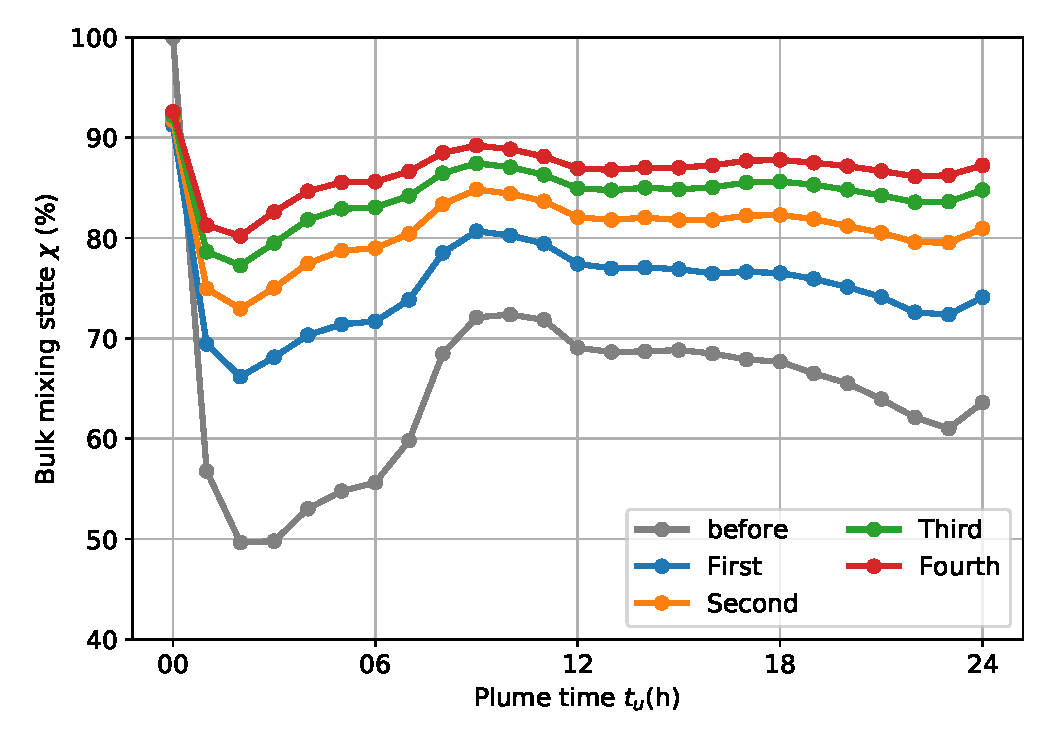
\includegraphics[scale=0.43]{chap5_figs/chap5-fig1.pdf}
    \caption{Evolution of bulk mixing state
      $\chi$ ($\%$) at the beginning of cloud cycle 1 and after each
      of the four cloud cycles.}
    \label{chap5-fig1}
\end{figure}

{\bf Quantifying the error in aerosol optical properties incurred by
  the internal mixture assumption.} I quantified the errors introduced
by the internal-mixture-assumption used in sectional aerosol
models. Using a size-resolved aerosol representation generally led to
an overestimation of volume absorption coefficients and an
underestimation of the volume scattering coefficients. The errors were
larger for externally mixed populations, as one might expect. For
absorption, the relative error reached up to 70\% for dry aerosol
populations. These magnitudes are comparable to the ones
\citet{Ching2017} found for the errors in CCN, as shown in
Fig~\ref{chap5-fig2}. The magnitude of the error was smaller for the
scattering error, about half of the error in absorption.
The increased BC core size after composition-averaging
  was responsible for the absorption overestimation, and scattering
  underestimation. The perturbations of the refractive index of the
  coating also contributed to the scattering underestimation. 
SSA can be underestimated up to $-$22\% and higher underestimation was associated with
larger scattering underestimation.The
relative humidity and associated water uptake had little effect in
changing the optical value errors brought by the internal mixture
assumption.

\begin{figure}[H]
    %\centering
    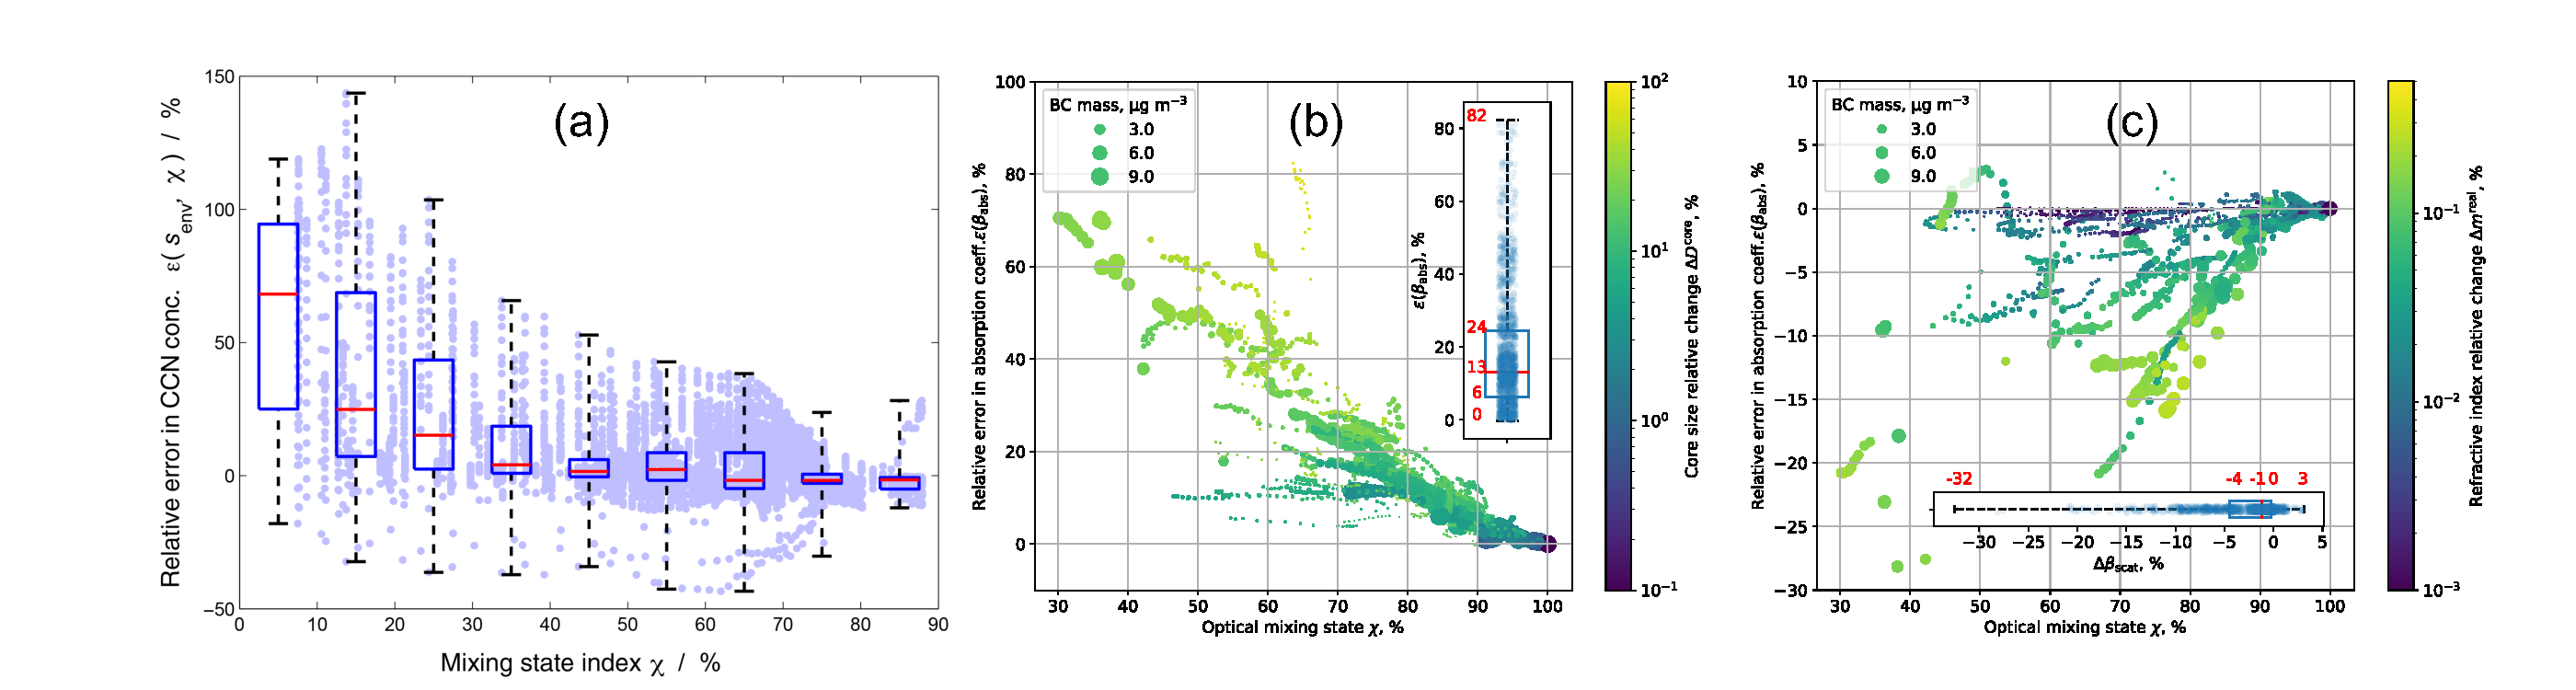
\includegraphics[scale=0.35]{chap5_figs/chap5-fig2.pdf}
    \caption{Relative error in (a) CCN concentration at
      supersaturation levels between 0.05\% to 1\%, (b) absorption
      coefficients and (c) scattering coefficients. (a) is adapted
      from \citet{Ching2017}. Check Fig.~\ref{fig3:abs-error} and
      Fig.~\ref{fig6:scat-err} in Chapter~\ref{chap4} for figure (b)
      and (c) details}
    \label{chap5-fig2}
\end{figure}

\section{Future work suggestions}
The findings presented in this thesis opened up several avenues for
further explorations.

{\bf Sensitivity of aqueous sulfate formation to per-particle
  properties.} I explored the capability of the particle-resolved
aqueous chemistry approach to simulate the aqueous sulfate reaction
systems. My simulation results confirm that the sulfate formation
catelyzed by TMI can be important, but I have not yet systematically
quantified the sensitivity of these processes to environmental
conditions. More simulations with varied conditions should be
conducted to generalized the cases with efficient TMI-catalyzed
sulfate formation and to highlight the relevance of mixing state for
these processes.

{\bf Improving the representation of cloud dynamics.} The adiabatic
cloud parcel model used for this thesis is very detailed in terms of
aerosol representation but very simplified in terms of representing
dynamical processes in the cloud. In particular, the mixing of the
in-cloud air with air from outside the cloud is currently not
included, but could be important because it changes the gas mixing
ratios and aerosol number concentrations within the cloud. Future work
could address this shortcoming and allow for a more realistic
representation of the interactions of aerosol and cloud chemistry and
cloud dynamics.

{\bf Considering the absorption of organic aerosol.} In the current
work, I did not consider the light absorption of organic
aerosol. Several recent studies have been devoted to constraining the
imaginary index values of brown carbon \citep{liu2020lifecycle}, and
\citet{Esteve2014} showed that the refractive index of organic
aerosols introduce large uncertainties in quantifying aerosol
absorbing abilities. Future work could incorporate these results and
quantify how the presence of absorbing organic aerosol modulates the
findings shown in this thesis.

{\bf Improving the representation of irregular shapes for
  BC-containing particles.}  I used Mie theory with core-shell
configuration to calculate optical properties, which relies on the
assumption of spherical particle shapes. Our results are therefore
most representative of BC-containing populations, where the BC core is
collapsed rather than a fractal aggregate \citep{china2013morphology,
  china2015morphology}. However, BC-containing particles with fractal
shape do exist in the atmosphere, and therefore more accurate methods,
such as discrete dipole approximation (DDA) should be used to
represent these more irregular particle shapes
\citep{scarnato2013effects,curtis2008laboratory,luo2019optical,
  wu2020light}.

{\bf Including dust and sea aerosol in calculations of optical
  properties errors.} For the simulations shown in Chapter~\ref{chap4}, I
focused on fine mode particles over urban regions. Sea salt and dust
particles were not included when creating the scenario library
populations. Considering the large coverage of the Earth with oceans
and deserts, it is also important to include these particle types when
evaluating the importance of mixing state for optical properties.

\appendix
% Reset the algorithm counter
\setcounter{algorithm}{0}

\chapter{Appendix to Chapter~\ref{chap2:mon}}
\label{tab:capram}
\section{List of aqueous reactions coupled to PartMC-MOSAIC}
This appendix shows the thermodynamic and kinetic data for the aqueous chemistry reactions 
coupled with PartMC-MOSAIC. It is based on the reduced CAPRAM 2.4 mechanism, 
and the full mecahnism can refer to \citet{Ervens2003}.
Table~\ref{Henry} lists the coefficients for Henry's Law.
%%%%%%%Table A1%%%%%%%%
\begin{table}[ht]
\centering
\caption{Henry's Law coefficients} \centering
\label{Henry}
\begin{threeparttable}
\begin{tabular}{ c l c c}
\toprule Henry's Law & Equilibrium & $K_{298}$ (M $\rm atm^{-1}$)$^*$& $-\Delta H/R$ (K) \\ 
\midrule
H1  & \ce{CO_2{(\rm g)}  <=> CO_2{(\rm aq)}} & 3.1$\times 10^{-2}$& 2423 \\ 
H2 & \ce{O_3{(\rm g)} <=> O_3{(\rm aq)}} &1.14 $\times 10^{-2}$ & 2300 \\ 
H3  & \ce{HO_2{(\rm g)}  <=> HO_2{(\rm aq)}} & 9.0$\times 10^{3}$& 0 \\ 
H4  & \ce{OH{(\rm g)}  <=> OH{(\rm aq)}} & 25 & 5280 \\ 
H5  & \ce{H_2O_2{(\rm g)} <=> H_2O_2{(\rm aq)}} &1.02 $\times 10^{5}$ & 6340 \\ 
H6  &\ce{NO_2{(\rm g)} <=> NO_2{(\rm aq)}} &1.2 $\times 10^{-2}$ & 1263\\
H7  &\ce{HONO{(\rm g)} <=> HONO{(\rm aq)}} & 49 & 4880\\
H8  & \ce{HNO_3{(\rm g)} <=> NO_3^- + H^+} &4.62 $\times 10^{6}$& 10500\\
H9  &\ce{NO_3{(\rm g)} <=> NO_3{(\rm aq)}} &6 $\times 10^{-1}$ & 0\\ 
H10  &\ce{N_2O_5{(\rm g)} <=> N_2O_5{(\rm aq)}} &1.4 $\times 10^{0}$ & 0\\ 
H11 & \ce{NH_3{(\rm g)}  <=> NH_3{(\rm aq)}} & 60.7 & 3920 \\ 
H12 & \ce{HCL{(\rm g)}  <=> CL^{-} + H^{+}} & 1.89$\times 10^6$ & 8910 \\ 
H13 & \ce{HCHO{(\rm g)}  <=> HCHO{(\rm aq)}} & 2.5 & 7216 \\ 
H14 & \ce{ORA{1}{(\rm g)}  <=> ORA{1}{(\rm aq)}} & 5.53$\times 10^3$ & 5630 \\ 
H15 &\ce{SO2{(\rm g)}  <=> SO2{(\rm aq)}} & 1.24 & 3247  \\ 
H16 &\ce{OP{1}{(\rm g)}  <=> OP{1}{(\rm aq)}} & 310 & 5607  \\ 
H17 &\ce{ORA{2}{(\rm g)}  <=> ORA{2}{(\rm aq)}} & 5.5$\times 10^3$ & 5890  \\ 
H18 &\ce{MO{2}{(\rm g)}  <=> MO{2}{(\rm aq)}} & 310 & 5607  \\ 
H19 &\ce{ETHPX{(\rm g)}  <=> ETHPX{(\rm aq)}} & 340 & 87  \\ 
H20 &\ce{ETOH{(\rm g)}  <=> ETOH{(\rm aq)}} & 190 & 6290  \\ 
H21 &\ce{CH{3}OH{(\rm g)}  <=> CH{3}OH{(\rm aq)}} & 220 & 5390  \\ 
H22 &\ce{ALD{(\rm g)}  <=> ALD{(\rm aq)}} & 4.8 & 6254  \\ 
H23 &\ce{BR{2}{(\rm g)}  <=> BR{2}{(\rm aq)}} & 0.758 & 3800  \\ 
H24 &\ce{CL{2}{(\rm g)}  <=> CL{2}{(\rm aq)}} & 9.15$\times 10^{-2}$ & 2490  \\ 
H25 &\ce{SULF{(\rm g)}  <=> HSO_4^- + H^{+}} & 8.7$\times10^{14}$ & 0 \\
H26 &\ce{HNO4{(\rm g)}  <=> HNO4{(\rm aq)}} &3$\times 10^4$& 0 \\ 
H27 &\ce{ACO3{(\rm g)}  <=> ACO3{(\rm aq)}} &6.69$\times 10^2$& 5893 \\ 
H28 &\ce{GLY{(\rm g)}  <=> GLY{(\rm aq)}} &1.40& 0 \\ 
H29 &\ce{[O_2]^{**}{(\rm g)}  <=> O_2{(\rm aq)}} &1.3$\times 10^{-3}$& 1700 \\ 
\bottomrule
\end{tabular}
\end{threeparttable}
\end{table}

% Table continued on next page
\addtocounter{table}{-1}
\begin{table}[ht]
\centering
\begin{threeparttable}
\caption{Continued.}
\begin{tabular}{ c l c c}
\toprule Henry's Law & Equilibrium & $K_{298}$ (M $\rm atm^{-1}$) & $-\Delta H/R$ (K) \\ 
\midrule
H30 &\ce{CLNO2{(\rm g)}  <=> CLNO2{(\rm aq)}} &0.024& 0.0 \\ 
H31 &\ce{BRNO2{(\rm g)}  <=> BRNO2{(\rm aq)}} & 0.3 & 0.0 \\ 
H32 &\ce{BRCL{(\rm g)}  <=> BRCL{(\rm aq)}} &0.94& 0.0 \\ 
H33 &\ce{NO{(\rm g)}  <=> NO{(\rm aq)}} &1.9$\times 10^{-3}$& 0.0 \\ 
\bottomrule
%\vspace*{5mm}
\end{tabular}
\begin{tablenotes}[para,flushleft]
      \small
      \item $*$: $K = K_{298} {\rm exp}(-\frac{\Delta H}{R}(\frac{1}{T}- \frac{1}{298}))$\\
      \item $**$: Specie with square bracket indicates its concentration is constant. 
\end{tablenotes}
\end{threeparttable}
\end{table}

Table~\ref{aq-ox} lists the coefficients for aqueous chemical reactions. 
%%%%%%Table A2%%%%%%%%%%%%
\begin{table}[ht]
\centering
\caption{Aqueous chemical reactions} \centering
\label{aq-ox}
\begin{threeparttable}
\begin{tabular}{ c l c c}
\toprule Aqueous chemistry & Reaction & $ K_{298}$ (${\rm M}^{-n}$ $\rm s^{-1}$) & $-E/R$ (K) \\ 
\midrule
A1 & \ce{FEOH^{2+} -> FE^{2+} + OH(\rm aq)} & 4.76$\times 10^{-3}$ & 2.20 \\
A2 & \ce{NO3^{-} -> NO2(\rm aq) + OH(\rm aq) + OH^{-}}& 4.57$\times 10^{-7}$ & 2.59 \\
A3 & \ce{H2O2(\rm aq) -> OH(\rm aq) + OH(\rm aq)} & 7.64$\times 10^{-6}$ & 2.46 \\
A4 & \ce{FEC2(O4)_2^{-} -> FE^{2+} + C2O4^{2-} + CO2(\rm aq) + CO2^{-}} &2.47 $\times 10^{-2}$& 1.96 \\
A5 & \ce{H2O2(\rm aq) + FE^{2+} -> FE^{3+} + OH(\rm aq) + OH^{-}} & 50.0 & 0.0 \\
A6 & \ce{H2O2(\rm aq) + Cu^+ -> Cu^{2+} + OH(\rm aq) + OH^-} & 7000.0 & 0.0 \\
A7 & \ce{O2^- + FE^{3+} -> FE^{2+} + O2(\rm aq)} & 1.5$\times 10^8$ & 0.0 \\
A8 & \ce{HO2(\rm aq) + FE(OH)^{2+} -> FE^{2+} + O2(\rm aq) + [H2O](\rm aq)} &1.3$\times 10^5$& 0.0 \\
A9 & \ce{O2^{-}(\rm aq) + FE(OH)^{2+} -> FE^{2+} + O_2(\rm aq) + OH^-} & 1.5$\times 10^8$ & 0.0 \\
A10 & \ce{O2^- + FE^{2+} -> FE^{3+} + H2O2(aq) + 2OH^- - 2[H2O](aq)} & 1.0$\times 10^7$ & 0.0 \\
A11 & \ce{HO2(aq) + FE^{2+} -> FE^{3+} + H2O2(aq) + 2OH^- -2[H2O](aq)} & 1.2$\times 10^6$& --5050.0 \\
A12 & \ce{OH(aq) + FE^{2+} -> FE(OH)^{2+}} & 4.3$\times 10^8$ & --1100 \\
A13 & \ce{O2^- + Cu^+ -> Cu^{2+} + H2O2(aq) + 2OH^- -2[H2O](aq)} & 1.0$\times 10^{10}$& 0.0 \\
A14 & \ce{HO2(aq) + Cu^+ -> Cu^{2+} + H2O2(aq) + OH^- -[H2O](aq)} & 2.3$\times 10^9$& 0.0 \\
A15 & \ce{HO2(aq) + Cu^{2+} -> Cu^+ + O2(aq) + H^+} & 1.0$\times 10^8$ & 0.0 \\
A16 & \ce{O2^- + Cu^{2+} -> Cu^+ O2(aq)} & 8$\times 10^9$ & 0.0 \\
A17 & \ce{FE^{3+} + Cu^+ ->= FE^{2+} + Cu^{2+}} & 1.3$\times 10^7$ & 0.0\\
A18 & \ce{FE(OH)^{2+} + Cu^+ -> FE^{2+} + Cu^{2+} + OH^-} & 1.3$\times 10^7$ & 0.0 \\
A19 & \ce{O3(\rm aq) + O2^- -> O3^- + O2(rm aq)} & 1.5$\times 10^9$ & 0.0 \\
A20 & \ce{HO3(aq) -> OH(\rm aq) + O2(\rm aq)} & 330.0 & --4500.0 \\
A21 & \ce{H2O2{(\rm aq)} + OH{(\rm aq)} -> HO_2{(\rm aq)} + H_2O} &3.0 $\times 10^{7}$& --1680 \\  
A22 & \ce{HSO3^- + OH{(\rm aq)} -> SO3^{-} + H2O}&2.7 $\times 10^{9}$& 0 \\ 
A23 & \ce{Cu^+ + O2(\rm aq) -> Cu^{2+} + O2^-} & 4.6$\times 10^5$& 0.0 \\
A24 & \ce{FE^{2+} + O3(aq) -> FEO^{2+} + O2(aq)} & 8.2$\times 10^5$ & --4690.0 \\
A25 & \ce{FEO^{2+} + Cl^- -> FE^{3+} + CLOH^- + OH^- - [H2O](aq)} & 100.0 & 0.0 \\
\bottomrule
\end{tabular}
\end{threeparttable}
\end{table}

% Table continued on next page
\addtocounter{table}{-1}
\begin{table}[ht]
\centering
\begin{threeparttable}
\caption{Continued.}
\begin{tabular}{ c l c c}
\toprule Aqueous chemistry & Reaction & $ K_{298}$ (${\rm M}^{-n}$ $\rm s^{-1}$) & $-E/R$ (K) \\ 
\midrule
A26 & \ce{FEO^{2+} + FE^{2+} -> 2FE^{3+} + 2OH^-} & 7.2$\times 10^4$ & --842.0 \\
A27 & \ce{N2O5(aq) -> NO2^+ + NO3^-} & 1.0$\times 10^9$ & 0.0 \\
A28 & \ce{NO2^+ + [H2O](aq) -> NO3^- + H^+ + SO3^-} & 8.9$\times 10^7$ & 0.0 \\
A29 & \ce{NO3(aq) + HSO3^-  -> NO3^- + H^+ + SO3^-} &1.3 $\times 10^{9}$& --2000.0\\ 
A30 & \ce{NO3(aq) + SO4^{2-}  -> NO3^- + SO4^-} & 1.0 $\times 10^{5}$& 0.0\\
A31 & \ce{NO4^-  -> NO2^- + O2{\rm (aq)}} & 4.5$\times10^{-2}$ & 0.0 \\ 
A32 & \ce{HNO4{(aq)} + HSO3^- -> HSO4^- + H^+ + NO3^-} &3.3 $\times 10^{5}$& 0.0 \\ 
A33 & \ce{NO2^+ + Cl^- -> CLNO2(aq)} & 1.0$\times 10^{10}$& 0.0 \\
A34 & \ce{NO2^+ + Br^- -> BRNO2(aq)} & 1.0$\times 10^{10}$& 0.0 \\
A35 & \ce{CLNO2(aq) + Br^- -> NO2^- + BRCL(aq)} & 5.0$\times 10^6$ & 0.0 \\
A36 & \ce{BRNO2(aq) + Br^- -> BR2(aq) + NO2^-} & 2.55$\times 10^4$ & 0.0 \\
A37 & \ce{BRNO2(aq) + Cl^- -> NO2^- + BrCl(aq)} & 10.0 & 0.0 \\
A38 & \ce{HMS^- + OH(aq) -> CHOHSO3^- + [H2O](aq)} & 3.0$\times 10^8$ & 0.0 \\
A39 & \ce{O2CHOHSO3^- + O2(aq) -> O2CHOHSO3^-} & 2.6$\times 10^9$& 0.0 \\
A40 & \ce{O2CHOHSO3^- -> HO2(aq) + CHOSO3^-} & 1.7$\times 10^4$ & 0.0 \\
A41 & \ce{O2CHOHSO3^- -> O2CHO(aq) + HSO3^-} & 7$\times 10^3$ & 0.0 \\
A42 & \ce{CHOSO3^- + [H2O](aq) -> HSO3^- + ORA{1}(aq)} & 1.26$\times 10^{-2}$ & 0.0 \\
A43 & \ce{O2CHO(aq) + [H2O](aq) -> ORA{1}(aq) + HO2(aq)} & 44.32 & 0.0 \\
A44 & \ce{HSO3^- + H2O2{(aq)} + H^+ -> SO4^{2-} + 2H^+ + [H2O](aq)} &7.2 $\times 10^{7}$& $-$4000.0\\ 
A45 & \ce{HSO3^- + O3{(aq)} -> SO4^{2-} + H^+ + O2{(aq)}} &3.7 $\times 10^{5}$& $-$5530.0 \\ 
A46 & \ce{SO3^{2-} + O3{(aq)} -> SO4^{2-} + O2{(aq)}} &1.5 $\times 10^{9}$& $-$5280.0 \\ 
A47 & \ce{SO5^{-} + FE^{2+} -> HSO5^- + FEOH^{2+}} & 2.65 $\times 10^7$ & -- 5809.0 \\
A48 & \ce{HSO5^- + FE^{2+} -> SO4^- + FEOH^{2+}} & 3.0$\times 10^4$ & 0.0 \\
A49 & \ce{FE^{2+} + SO4^- -> FEOH^{2+} + SO4^{2-} + H^+} & 4.6$\times 10^9$ & 2165.0 \\
A50 & \ce{SO5^- + SO5^- -> SO4^- + SO4^- + O2(aq)} & 2.2 $\times 10^8$ & --2600.0 \\ 
A51 & \ce{SO5^- + HO2{(aq)} -> SO5O2H^-} & 1.7$\times 10^9$ & 0.0 \\
A52 & \ce{SO5O2^{2-} -> HSO5^- + O2(aq) + OH^- -[H2O](aq)} & 1.2$\times 10^3$ & 0.0 \\
A53 & \ce{SO3^- + O2{(\rm aq)} -> SO5^-} & 2.5$\times10^9$ & 0.0 \\ 
A54 & \ce{SO4^- + [H_2O](aq) -> SO4^{2-} + OH{(\rm aq)} + H^+} & 11.0 & -1110.0 \\
A55 & \ce{HSO5^- + HSO3^- + H^+ -> 2SO4^{2-} + 3H^+ } & 7.14$\times 10^6$& 0.0 \\
A56 & \ce{CH3OH(aq) + OH(aq) -> CH2OH(aq) + [H2O](aq)} & 1.0$\times 10^9$ & 0.0 \\
A57 & \ce{CH2OH(aq) + O2(aq) -> O2CH2OH(aq)} & 2 $\times 10^9$ & 0.0 \\
A58 & \ce{O2CH2OH(aq) + O2CH2OH(aq) -> CH2OH(aq) + O2(aq) + aHCHO} & 1.05$\times 10^9$ & 0.0 \\
A59 & \ce{ETOH(aq) + OH(aq) -> CH3CHOH(aq) + [H2O](aq)} & 1.9$\times 10^9$ & 0.0 \\
A60 & \ce{CH3CHOH(aq) + O2(aq) -> O2CH3CHOH(aq)} & 2.0$\times 10^9$ & 0.0 \\
A61 & \ce{O2CH3CHOH(aq) + ALD(aq) -> HO2(aq)} & 52.0 & --7217.0 \\
A62 & \ce{CH2OH2(aq) + OH(aq) -> CHOH2(aq) + [H2O](aq)} & 1.0 $\times 10^9$ & --1020.0 \\
A63 & \ce{CHOH2(aq) + O2(aq) -> HO2(aq) + ORAQ1(aq)} & 2.0$\times 10^9$ & 0.0 \\
A64 & \ce{CH3CHOH2(aq) + OH(aq) -> CH3COH2(aq) + [H2O](aq)} & 1.2$\times 10^9$ & 0.0 \\
A65 & \ce{ALD(aq) + OH(aq) -> CH3CO(aq) + [H2O](aq)} & 3.6$\times 10^9$ & 0.0 \\
A66 & \ce{ORA{1}(aq) + OH(aq) -> CO2H(aq) + [H2O](aq)} & 1.3$\times 10^8$ & $-1000.0$ \\
A67 & \ce{HCOO^- + OH(aq) -> CO2H(aq) + OH^-} & 3.2 $\times 10^9$ & $-1000.0$ \\
A68 & \ce{ORA2(aq) + OH(aq) -> CH2COOH(aq) + [H2O](aq)} & 1.5$\times 10^7$ & $-1330.0$ \\
A69 & \ce{MCOO^- + OH(aq) -> CH2COO^- + [H2O](aq)} & 1.5$\times 10^7$ & --1800.0 \\
A70 & \ce{CH2COOH(aq) + O2(aq) -> ACO3(aq)} & 1.7 $\times 10^9$ & 0.0 \\
A71 & \ce{MO2(aq) + MO2(aq) -> CH3OH(aq) + HCHO(aq) + O2(aq)} & 7.4$\times 10^7$ & 0.0 \\
A72 & \ce{MO2(aq) + MO2(aq) -> Ch3O(aq) + CH3O(aq) + O2(aq)} & 3.6$\times 10^7$ & --2200.0 \\
A73 & \ce{ACO3(aq) + ACO3(aq) -> 2MO2(aq) + 2CO2(aq) + O2(aq)} & 1.5$\times 10^8$ & 0.0 \\
A74 & \ce{MO2(aq) + HSO3^- -> OP1(aq) + SO3^-} & 5.0$\times 10^5$ & 0.0\\
\bottomrule
%\vspace*{5mm}
\end{tabular}
\end{threeparttable}
\end{table}

% Table continued on next page
\addtocounter{table}{-1}
\begin{table}[ht]
\centering
\begin{threeparttable}
\caption{Continued.}
\begin{tabular}{ c l c c}
\toprule Aqueous chemistry & Reaction & $ K_{298}$ (${\rm M}^{-n}$ $\rm s^{-1}$) & $-E/R$ (K) \\ 
\midrule
A75 & \ce{ETHPX(aq) + ETHPX(aq) -> CH3CH2O(aq) + CH3CH2O(aq) + O2(aq)} & 1.0$\times 10^8$ & 750.0 \\
A76 & \ce{CH3CH2O(aq) -> CH3CHOH(aq)} & 1.0$\times 10^6$ & 0.0 \\
A77 & \ce{OH(aq) + HC2O4^- -> C2O4^- + [H2O](aq)} & 3.2$\times 10^7$ & 0.0 \\
A78 & \ce{OH(aq) + C2O4^{2-} -> OH^- + C2O4^-} & 5.3$\times 10^6$ & 0.0 \\
A79 & \ce{C2O4^- + O2(aq) -> CO2(aq) + O2^- + CO2(aq)} & 2$\times 10^9$ & 0.0 \\
A80 & \ce{OH(aq) + CHOH2CHOH2(aq) -> COH2CHOH2(aq) + [H2O](aq)} &1.1$\times 10^9$  & --1516.0 \\
A81 & \ce{COH2CHOH2(aq) + O2(aq) -> aO2COH2CHOH2(aq)} & 1.38$\times 10^9$ & 0.0 \\
A82 & \ce{O2COH2CHOH2(aq) -> HO2(aq) + CHOH2COOH(aq)} & 2$\times 10^9$ & 0.0\\
A83 & \ce{HO(aq) + CHOH2COOH(aq)  ->  COH2COOH(aq) + [H2O](aq)} & 1.1$\times 10^9$& --1516.0 \\
A84 & \ce{COH2COOH(aq) + O2(aq) -> O2COH2COOH(aq)} & 2.0$\times 10^9$ & 0.0 \\
A85 & \ce{O2COH2COOH(aq)  -> HO2(aq) + H2C2O4(aq)} & 2.0$\times 10^9$ & 0.0 \\
A86 & \ce{CH3COH2(aq) + O2(aq) -> CH3COH2OO(aq)} & 2.0$\times 10^9$& 0.0 \\
A87 & \ce{CH3COH2OO(aq) -> H^+ + H^+ + MCOO^- + O2^-} & 1.0$\times 10^5$ & 0.0\\
A88 & \ce{CH3O(aq) -> CH2OH(aq)} & 1.0$\times 10^6$ & 0.0 \\
A89 & \ce{CH2COO^- + O2(aq) -> O2CH2COO^-} & 2.0$\times 10^9$ & 0.0 \\
A90 & \ce{O2CH2COO^- + O2CH2COO^- -> 2CHOH2COO^- + H2O2(aq)} & 2.0$\times 10^7$& 0.0\\
A91 & \ce{CO2^- + O2(aq) -> CO2(aq) + O2^-} & 4.0$\times 10^9$ & 0.0 \\
A92 & \ce{Cl2^- + FE^{2+} -> 2 Cl^- + FE^{3+}} & 1.0$\times 10^7$ & --3030.0 \\
A93 & \ce{Cl2^- + HO2(aq) -> 2Cl^- + H^+ + O2(aq)} & 1.3$\times 10^{10}$ & 0.0\\
A94 & \ce{Cl2^- + HSO3^- -> 2Cl^- + H^+ + SO3^-} & 1.7$\times 10^8$& --400.0 \\
A95 & \ce{Cl2(aq) + [H2O](aq) -> H^+ + Cl^- + HOCL(aq)} & 0.4 & --7900.0 \\
A96 & \ce{Cl2^- + [H2O](aq) -> H^+ + Cl^- + Cl^- + HO(aq)} & 23.4 & 0.0 \\
A97 & \ce{Br^- + SO4^- -> SO4^{2-} + Br(aq)} & 2.1$\times 10^9$ & 0.0 \\
A98 & \ce{Br^- + NO3(aq) -> NO3^- + Br(aq)} & 3.8$\times 10^9$ & 0.0 \\
A99 & \ce{Br2^- + Br2^- -> Br2(aq) + 2Br^} & 1.7$\times 10^9$ & 0.0 \\
A100 & \ce{Br2^- +  FE^{2+} -> 2Br^- + FE^{3+}} & 3.6$\times 10^6$ & --3330.0 \\
A101 & \ce{Br2^- + H2O2(aq) -> 2Br^- + H^+ + HO2(aq)} & 1.0$\times 10^5$ & 0.0 \\
A102 & \ce{Br2^- + HO2(aq) -> 2BR^- + O2(aq) + H^+} & 6.5$\times 10^9$ & 0.0 \\
A103 & \ce{Br2^- + HSO3^- -> 2BR^- + H^+ + SO3^-} & 5.0$\times 10^7$ & --780.0 \\
A104 & \ce{Br2(aq)  + [H2O](aq) -> H^+ + Br^- + HOBr(aq)} & 0.031 & --7500.0 \\
A105 & \ce{BrOH^- -> Br(aq) + OH^-} &4.2$\times 10^6$ &0.0 \\
\bottomrule
%\vspace*{5mm}
\end{tabular}
\end{threeparttable}
\end{table}

Table~\ref{aq-equi} lists constants for equilibrium equations. 

\begin{table}[ht]
\centering
\caption{Equilibrium reactions} \centering
\label{aq-equi}
\begin{threeparttable}
\begin{tabular}{ c l c c}
\toprule Aqueous equilibria & Reaction & $K_{298}$ (${\rm M}^{-n}$ $\rm s^{-1}$) & $-\Delta(H)/R$ (K) \\ 
\midrule
D1 & \ce{H_2O{(aq)} <=> OH^- + H^+} &1.8 $\times 10^{-16}$& --6800.0\\
D2 & \ce{CO_2{(aq)} <=> HCO_3^- + H^+} & 4.3 $\times 10^{-7}$& --913.0\\
D3 & \ce{NH_3{(aq)} + H_2O <=>  NH_4^+ + OH^-} &3.17 $\times 10^{-7}$& --560.0 \\
D4 & \ce{HO_2{(aq)} <=> O_2^- + H^+} & 1.6$\times 10^{-5}$& 5.0$\times 10^{10}$\\
D5 & \ce{HONO(aq) <=> NO2^- + H^+} & 5.3$\times 10^{-4}$ & --1760.0 \\
D6 & \ce{HNO_4{(\rm aq)} <=> NO_4^- + H^+} & 1$\times 10^{-5}$& 5$\times 10^{10}$ \\
D7 & \ce{NO_2{(\rm aq)} + HO_2{(\rm aq)} <=>  HNO_4{(\rm aq)}} &2.2 $\times 10^{9}$ &4.6$\times 10^{-3}$ \\
D8 & \ce{SO_2{(\rm aq)} + H_2O <=>  HSO_3^- + H^+} &3.13 $\times 10^{-4}$& 1940.0 \\
D9 & \ce{HSO_3^- <=>  SO_3^{2-} + H^+} &6.22 $\times 10^{-8}$& 1960.0\\
D10 & \ce{HSO_4^- <=> H^+ + SO_4^{2-}} &1.02$\times 10^{-2}$& 2700.0\\
D11 & \ce{ORA{1}(aq) <=> H^+ + HCOO^-} & 1.77$\times 10^{-4}$ & 12.0 \\
D12 & \ce{ORA{2}(aq) <=> H^+ + MCOO^-} & 1.75$\times 10^{-5}$ & 46.0 \\
D13 & \ce{FE^{3+} + [H2O](aq) <=> FEOH^{2+} + H^+} & 1.1$\times 10^{-4}$ & 4.3$\times 10^8$ \\
D14 & \ce{HCHO(aq) + [H2O](aq) <=> CH2OH2(aq)} & 36.0 & 4030.0 \\
D15 & \ce{ALD(aq) + [H2O](aq) = CH3CHOH2(aq)} & 2.46$\times 10^{-2}$& 2500.0 \\
D16 & \ce{HSO3^- + HCHO(aq) <=> HMS^-} & 790.0 & --3293.0 \\
D17 & \ce{HMS^- <=> HSO3^-  + HCHO(aq)} & 1.197$\times 10^{-7}$ & --5831.0 \\
D18 & \ce{SO3^{2-} + HCHO(aq) <=> HMS^- + OH^- - [H2O](aq)} & 2.5$\times 10^7$ & --2752.0 \\
D19 & \ce{HMS^ <=> HCHO(aq) + SO3^{2-} + H^+} & 3.79$\times 10^{-3}$& --5290.0 \\
D20 & \ce{Cl(aq) + Cl^- <=> Cl2^-} & 1.4$\times 10^5$ & 6$\times 10^4$ \\
D21 & \ce{Br + Br^- <=> Br2^-} & 6.32$\times 10^5$ & 1.9$\times 10^4$ \\
D22 & \ce{Cl^- + HO(aq) <=> ClOH^-} & 0.7 & 6.1$\times 10^9$ \\
D23 & \ce{ClOH^- + H^+ <=> Cl(aq) + [H2O](aq)} & 5.1$\times 10^6$& 4100.0 \\
D24 & \ce{Br^- + HO(aq) <=> BrOH^-} & 333.0 & 3.3$\times 10^7$ \\
D25 & \ce{BrOH^- + H^+ <=> Br(aq) + [H2O](aq)} &1.8$\times 10^{12}$ & 2.45$\times 10^{-2}$ \\
D26 & \ce{HO3(aq) <=> H^+ + O3^-} & 6.3$\times 10^{-9}$ & 5.2$\times 10^{10}$ \\
D27 & \ce{CHOHSO3^-  <=> CHOSO3^{2-} + H^+} & 1.34$\times 10^{-6}$ &4.4$\times 10^{10}$ \\
D28 & \ce{SO5O2H^- <=>  H^+ + SO5O2^{2-}} & 1.5$\times 10^{-5}$ & 5.0$\times 10^{10}$ \\
D29 & \ce{HC2O4m = C2O4mm + Hp} <=> & 6.25$\times 10^{-5}$ & 5.0$\times 10^{10}$ \\
D30 & \ce{H2C2O4(aq) <=> HC2O4^- + H^+} & 6.4$\times 10^{-2}$& 5.0$\times 10^{10}$ \\
D31 & \ce{CHOH2COOH(aq) <=> H^+ + CHOH2COO^-} & 3.16$\times 10^{-4}$ & 2.0$\times 10^{10}$ \\
D32 & \ce{GLY(aq) + [H2O](aq) <=>  CHOH2CHOH2(aq)} & 3900.0 & 5.5$\times 10^{-3}$ \\
D33 & \ce{FE^{3+} + C2O4^{2-} = FEC2O4^+} &2.9$\times 10^9$ & 3.0$\times 10^{-3}$ \\
D34 & \ce{FEC2O4^+ + C2O4^{2-} <=> FEC2(O4)2^-} & 6.3$\times 10^6$ & 3.0$\times 10^{-3}$ \\
D35 & \ce{SO4^- + CL^- <=> SO4^{2-} + CL(aq)} & 1.2 & 2.1$\times 10^8$ \\
D36 & \ce{NO3(aq) + CL^- <=> NO3^- + CL(aq)} & 3.4 & --4300 \\
D37 & \ce{CH3CO(aq) + [H2O](aq) <=> CH3COH2(aq)} & 367.0 & 0.0 \\
D38 & \ce{ACO3(aq) <=> H^+ + O2CH2COO^-} & 1.75$\times 10^{-5}$ & 46.0 \\
D39 & \ce{Na^+ + Na^+_C <=> Na^+ + Na^+_C} & 0.0 & 0.0\\
\bottomrule
\end{tabular}
\end{threeparttable}
\end{table}

\chapter{Appendix to Chapter~\ref{chap3}}
\label{tab:AppB}
\begin{ThreePartTable}
  \begin{TableNotes}
    \raggedright
    \begin{hyphenrules}{nohyphenation}
    \item[]
    *: Note that Henry's Law partitioning is treated kinetically with an uptake rate constant 
     calculated as in equation 1 of Ervens et al. (2003), and then using the equilibrium constant 
     to calculate the evaporation rate constant.
    \end{hyphenrules}
  \end{TableNotes}
\begin{longtable}{ c l c c} 

	%\settablenum{S1}
	%\centering
	\caption{Thermodynamic and kinetic data for a subset of CAPRAM 2.4 mechanism} \\
	\hline
	Henry's Law & Equilibrium & $K_{298}^*$ (M $\rm atm^{-1}$) & $-\Delta H/R$ (K) \\ 
	\hline
	\endfirsthead
	
	\caption{Thermodynamic and kinetic data for a subset of CAPRAM 2.4 mechanism (Continued)} \\
	%\centering 
	\hline
 	Aqueous equilibria & Reaction & $K$ (${\rm M}$) & $-\Delta H/R$ (K) \\ 
 	\hline
	\endhead
	
	\hline \multicolumn{3}{r}{{Continued}} \\ 
	
	\hline \endfoot
	
	\insertTableNotes
	\endlastfoot
		
	H1  & \ce{CO_2{(\rm g)}  <=> CO_2{(\rm aq)}} & 3.1$\times 10^{-2}$& 2423 \\ 
	H2  & \ce{O_3{(\rm g)} <=> O_3{(\rm aq)}} &1.14 $\times 10^{-2}$ & 2300 \\ 
	H3  & \ce{HO_2{(\rm g)}  <=> HO_2{(\rm aq)}} & 1.14$\times 10^{-2}$& 2300 \\ 
	H4  & \ce{OH{(\rm g)}  <=> OH{(\rm aq)}} & 9$\times 10^{3}$& 0 \\ 
	H5  & \ce{H_2O_2{(\rm g)} <=> H_2O_2{(\rm aq)}} &1.02 $\times 10^{5}$ & 6340 \\ 
	H6  &\ce{NO_2{(\rm g)} <=> NO_2{(\rm aq)}} &1.2 $\times 10^{-2}$ & 1263\\ 
	H7  & \ce{HNO_3{(\rm g)} <=> NO_3^- + H^+} &4.62 $\times 10^{6}$& 10500\\
	H8  &\ce{NO_3{(\rm g)} <=> NO_3{(\rm aq)}} &6 $\times 10^{-1}$ & 0\\ 
	H9  &\ce{N_2O_5{(\rm g)} <=> N_2O_5{(\rm aq)}} &1.4 $\times 10^{0}$ & 0\\ 
	H10 & \ce{NH_3{(\rm g)}  <=> NH_3{(\rm aq)}} & 60.7 & 3920 \\ 
	H11 & \ce{HCL{(\rm g)}  <=> CL^{-} + H^{+}} & 1.89$\times 10^6$ & 8910 \\ 
	H12 &\ce{SO_2{(\rm g)}  <=> SO_2{(\rm aq)}} & 1.24 & 3247  \\ 
	H13 &\ce{SULF{(\rm g)}  <=> HSO_4^- + H^{+}} & 8.7$\times10^{14}$ & 0 \\
	H14 &\ce{HNO_4{(\rm g)}  <=> HNO_4{(\rm aq)}} &3$\times 10^4$& 0 \\ 
	H15 &\ce{O_2{(\rm g)}  <=> O_2{(\rm aq)}} &1.3$\times 10^{-3}$& 1700 \\ 
	H16 &\ce{NO{(\rm g)}  <=> NO{(\rm aq)}} &1.9$\times 10^{-3}$& 0 \\ 
	\hline
	Aqueous equilibria & Reaction & $K$ (${\rm M}$) & $-\Delta H/R$ (K) \\ 
	\hline
	D1 & \ce{H_2O{(\rm aq)} <=> OH^- + H^+} &1.8 $\times 10^{-16}$& --6800\\
	D2 & \ce{CO_2{(\rm aq)} <=> HCO_3^- + H^+} & 1.72 $\times 10^{6}$& --913\\
	D3 & \ce{NH_3{(\rm aq)} + H_2O(aq) <=>  NH_4^+ + OH^-} &3.17 $\times 10^{-7}$& --560 \\
	D4 & \ce{HO_2{(\rm aq)} <=> O_2^- + H^+} & 3.17$\times 10^{-7}$& 5.0$\times 10^{10}$\\
	D5 & \ce{HNO_4{(\rm aq)} <=> NO_4^- + H^+} & 1$\times 10^5$& 5.0$\times 10^{10}$ \\
	D6 & \ce{NO_2{(\rm aq)} + HO_2{(aq)} <=>  HNO_4{(\rm aq)}} &2.2 $\times 10^{9}$ &4.6$\times 10^{-3}$ \\
	D7 & \ce{SO_2{(\rm aq)} + H_2O(aq) <=>  HSO_3^- + H^+} &3.13 $\times 10^{-4}$& 1940 \\
	D8 & \ce{HSO_3^- <=>  SO_3^{2-} + H^+} &6.22 $\times 10^{-8}$& 1960\\
	D9 & \ce{HSO_4^- <=> H^+ + SO_4^{2-}} &1.02$\times 10^{-2}$& 2700\\
	\hline
	Aqueous chemistry & Reaction & $ K_{298}$ (${\rm M}^{-n}$ $\rm s^{-1}$) & $-E/R$ (K) \\ 
	\hline
	A1  & \ce{H_2O_2{(\rm aq)} + OH{(\rm aq)} -> HO_2{(\rm aq)} + H_2O} &3.0 $\times 10^{7}$& $-$1680 \\  
	A2 & \ce{HSO_3^- + OH{(\rm aq)} -> SO_3^{-} + H_2O}&2.7 $\times 10^{9}$& 0 \\ 
	A3 & \ce{N_2O_5(\rm aq)  -> NO_3^- + NO_2^+} & 1.0 $\times 10^{9}$& 0 \\
	A4 & \ce{NO_2^+ + H_2O(aq) -> NO_3^- + H^+ + H^+} & 8.9 $\times 10^{7}$& 0 \\ 
	A5 & \ce{NO_3(\rm aq) + HSO_3^-  -> NO_3^- + H^+ + SO_3^-} &1.3 $\times 10^{9}$& --2000\\ 
	A6 & \ce{NO_3(\rm aq) + SO_4^{2-}  -> NO_3^- + SO_4^-} & 1.0 $\times 10^{5}$& 0\\
	A7 & \ce{NO_4^-  -> NO_2^- + O_2{\rm (aq)}} & 4.5$\times10^{-2}$ & 0 \\ 
	A8 & \ce{HNO_4{(\rm aq)} + HSO_3^- -> HSO_4^- + H^+ + NO_3^-} &3.3 $\times 10^{5}$& 0 \\ 
	A9 & \ce{HSO_3^- + H_2O_2{(\rm aq)} + H^+ -> SO_4^{2-} + 2H^+ + H_2O} &7.2 $\times 10^{7}$& $-$4000\\ 
	A10 & \ce{HSO_3^- + O_3{(\rm aq)} -> SO_4^{2-} + H^+ + O_2{(\rm aq)}} &3.7 $\times 10^{5}$& $-$5530 \\ 
	A11 & \ce{SO_3^{2-} + O_3{(\rm aq)} -> SO_4^{2-} + O_2{(\rm aq)}} &1.5 $\times 10^{9}$& $-$5280 \\ 
	A12 &\ce{SO_5^- + SO_5^- -> SO_4^- + SO_4^- +  O_2{(\rm aq)}} & 2.2$\times 10^8$ & $-$2600 \\
	A13 & \ce{SO_5^- + HO_2{(\rm aq)} -> SO_5O_2H^-} & 1.7$\times 10^9$ & 0 \\
	A14 & \ce{SO_3^- + O_2{(\rm aq)} -> SO_5^-} & 2.5$\times10^9$ & 0 \\ 
	A15 & \ce{SO_4^- + H_2O(aq) -> SO_4^{2-} + OH{(\rm aq)} + H^+} & 11 & -1110 \\
	A16 & \ce{HSO_5^- + HSO_3^- + H^+ -> 2SO_4^{2-} + 3H^+ } &7.14$\times 10^6$& 0 \\
	\hline
%\end{tabular}
    \label{tab:aqchem}
\end{longtable}
\end{ThreePartTable}
%\end{center}

\backmatter
\renewcommand{\bibname}{References}
\bibliographystyle{copernicus}
\bibliography{thesis_ref}
\end{document}
%\chapter{Appendix to Chapter~\ref{chap2:mon}}



